\باب{میدانی ٹرانزسٹر}

دو جوڑ ٹرانزسٹر کی طرح \اصطلاح {میدانی ٹرانزسٹر}\فرہنگ{میدانی ٹرانزسٹر} یا \اصطلاح {فیٹ}\فرہنگ{فیٹ}  \تحریر{FET} بھی اپنے دو سروں کے مابین برقی رو کا گزر قابو کرنے کی صلاحیت رکھتا ہے۔یوں انہیں بطور ایمپلیفائر یا برقی سوئچ استعمال کیا جا سکتا ہے۔\اصطلاح {میدانی ٹرانزسٹر} کے دو سروں کے مابین \اصطلاح {برقی میدان کی شدت}\حاشیہب{electric field intensity} اس میں برقی رو کے گزر کو قابو کرتا ہے۔اسی سے اس کا نام \اصطلاح {میدانی ٹرانزسٹر} نکلا ہے۔میدانی ٹرانزسٹر \عددی{n} یا \عددی{p} قسم کا بنانا ممکن ہوتا ہے۔\عددی{n} قسم \اصطلاح {فیٹ} میں برقی  رو کا گزر بذریعہ منفی \اصطلاح{برقی بار}\فرہنگ{برقی!بار}\فرہنگ{بار}\حاشیہب{charge}\فرہنگ{charge} جبکہ \عددی{p} قسم کے \اصطلاح {فیٹ} میں بذریعہ مثبت \اصطلاح{برقی بار} ہوتا ہے۔

میدانی ٹرانزسٹر کے کئی اقسام ہیں جن میں \اصطلاح {ماسفیٹ}\فرہنگ{ماسفیٹ} \تحریر{MOSFET}  سب سے زیادہ مقبول ہے۔بقایا اقسام کے ٹرانزسٹروں کے نسبت ماسفیٹ کا بنانا نسبتاً آسان ہے۔مزید یہ کہ ماسفیٹ کم رقبہ پر بنتا ہے اور یوں انہیں استعمال کرتے ہوئے سلیکان کی پتری  پر زیادہ گھنے ادوار بنانا ممکن ہوتا ہے۔مخلوط عددی ادوار صرف ماسفیٹ استعمال کرتے ہوئے تخلیق دینا ممکن ہے یعنی ایسے ادوار مزاحمت یا ڈایوڈ کے استعمال کے بغیر بنائے جا سکتے ہیں۔انہیں وجوہات کی بنا پر جدید \اصطلاح {عددی مخلوط ادوار}\حاشیہب{digital integrated circuits} مثلاً \اصطلاح {مائیکروپروسیسر}\حاشیہب{microprocessor}  اور \اصطلاح {حافظہ}\حاشیہب{memory}  ماسفیٹ سے ہی تخلیق دئے جاتے ہیں۔اس باب میں \اصطلاح {ماسفیٹ} \تحریر{MOSFET} پر بالخصوص اور \اصطلاح {جوڑ دار فیٹ} \تحریر{JFET} پر بالعموم غور کیا جائے گا۔

\حصہ{ \عددی{n} ماسفیٹ کی ساخت (بڑھاتا \عددی{n} ماسفیٹ)}
شکل \حوالہ{شکل_ماسفیٹ_کی_ساخت_منفی}  میں \عددی{n} ماسفیٹ بنتے ہوئے دکھایا گیا ہے۔اس شکل میں وضاحت کی غرض سے ماسفیٹ کے مختلف حصے بڑھا چڑھا کر دکھائے گئے ہیں جن کا ماسفیٹ کے حقیقی جسامت سے کوئی تعلق نہیں۔اگرچہ شکل میں سلیکان کی پتری کی موٹائی کو کم دکھایا گیا ہے حقیقت میں یہ ماسفیٹ کے جسامت سے اتنی موٹی ہوتی ہے کہ اس کے موٹائی کو ماسفیٹ کی جسامت کے لحاض سے لامحدود تصور کیا جاتا ہے۔
\begin{figure}
\centering
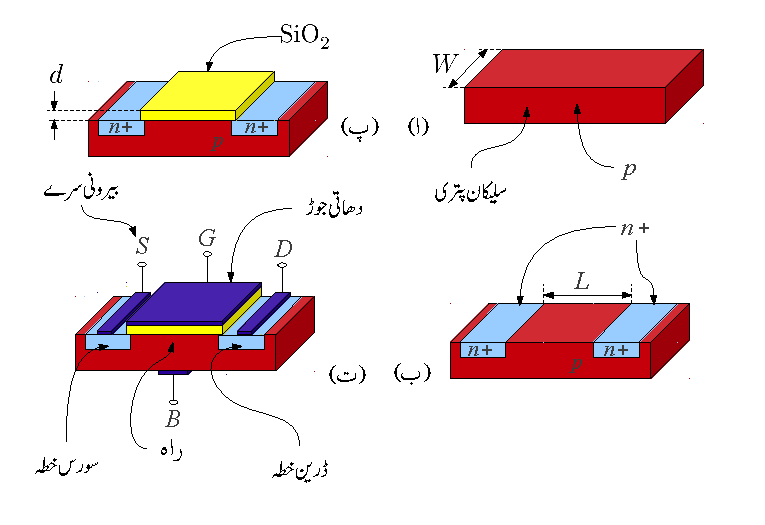
\includegraphics[scale=0.90]{nMOSFETstructure}
\caption{\عددی{n} ماسفیٹ کی ساخت}
\label{شکل_ماسفیٹ_کی_ساخت_منفی}
\end{figure}
شکل \حوالہ{شکل_ماسفیٹ_کی_ساخت_منفی} الف میں مثبت یعنی \عددی{p} قسم کے سلیکان\حاشیہب{silicon} کی پتری جس کی چوڑائی \عددی{W} ہے سے شروع کیا گیا ہے۔سلیکان پتری کی موٹائی ماسفیٹ کے وجود سے بہت زیادہ ہوتی ہے لہٰذا سلیکان پتری کی موٹائی کو لامحدود تصور کیا جاتا ہے۔جیسا شکل  ب میں دکھایا گیا ہے، اس پتری میں دو جگہ \اصطلاح {دوری جدول}\حاشیہب{periodic table}  کے پانچویں گروہ، یعنی \عددی{n} قسم کے ایٹموں کے نفوذ سے ملاوٹ کر کے  \عددی{n+} خطے بنائے گئے ہیں۔ان خطوں میں  \عددی{n} ایٹموں کی عددی کثافت عام حالات سے کئی زیادہ  رکھی جاتی ہے۔اسی لئے انہیں \عددی{n} کے بجائے \عددی{n+} خطے کہا گیا ہے۔ان دو \عددی{n+}  خطوں کے مابین  فاصلہ \عددی{L} ہے۔شکل  پ میں \عددی{p} قسم کی سلیکان کی پتری کے اوپر، دو \عددی{n+} خطوں کے مابین \عددی{\mathrm{SiO_2}} اگایا جاتا ہے۔ \عددی{\mathrm{SiO_2}}  انتہائی بہتر غیر موصل ہے۔اگائے گئے \عددی{\mathrm{SiO_2}} کی موٹائی \عددی{d} ہے۔شکل  ت میں \عددی{n+} خطوں کے علاوہ  \عددی{\mathrm{SiO_2}} کے اوپر اور سلیکان پتری کے نچلے سطح پر  برقی جوڑ بنانے کی غرض سے دھات جوڑا گیا ہے۔ان چاروں دھاتی سطحوں کے ساتھ برقی تار جوڑ کر انہیں بطور ماسفیٹ کے بیرونی سروں کے استعمال کیا جاتا ہے۔ان بیرونی برقی سروں کو \اصطلاح {سورس} ، \اصطلاح {گیٹ}\حاشیہب{gate}، \اصطلاح {ڈرین} اور \اصطلاح {بدن}\فرہنگ{بدن}\حاشیہب{بدن سے مراد سلیکان کی پتری کا وجود ہے۔} کہا جائے گا اور انہیں \عددیء{\textup{S}}،   \عددیء{\textup{G}}، \عددی{\textup{D}} اور \عددی{\textup{B}} سے پہچانا جاتا ہے۔شکل \حوالہ{شکل_منفی_ماسفیٹ_کی_علامتیں} میں ماسفیٹ کی مختلف علامتیں دکھائی گئی ہیں۔عموماً \اصطلاح {بدن}\حاشیہب{body} کو سورس کے ساتھ جوڑ کر باہر ان دونوں کے لئے ایک ہی سرا نکالا جاتا ہے جسے \اصطلاح {سورس} تصور کیا جاتا ہے۔ایسی صورت میں ماسفیٹ کے تین سرے پائے جائیں گے۔شکل  پ میں اسی کی علامت دکھائی گئی ہے جہاں تیر کا نشان ماسفیٹ میں سے گزرتے برقی رو کی صحیح سمت دکھاتا ہے۔اس کتاب میں عموماً ماسفیٹ کو تین سروں کا ہی تصور کیا گیا ہے۔

\اصطلاح {بدن} اور ڈرین \عددی{pn} ڈایوڈ بناتے ہیں۔اسی طرح \اصطلاح {بدن} اور سورس بھی \عددی{pn} ڈایوڈ بناتے ہیں۔\اصطلاح {بدن} اور سورس کو ایک ساتھ جوڑنے سے \اصطلاح {بدن} اور سورس کے درمیان ڈایوڈ قصر دور ہو جاتا ہے اور ساتھ ہی ساتھ \اصطلاح {بدن} اور ڈرین کے درمیان ڈایوڈ سورس اور ڈرین کے درمیان جڑ جاتا ہے۔شکل \حوالہ{شکل_منفی_ماسفیٹ_کی_علامتیں} پ میں اگرچہ سورس سے ڈرین ڈایوڈ نہیں دکھایا گیا لیکن یہ یاد رکھنا ضروری ہے کہ ایسا ڈایوڈ پایا جاتا ہے۔اسے عموماً استعمال بھی کیا جاتا ہے۔
\begin{figure}
\centering
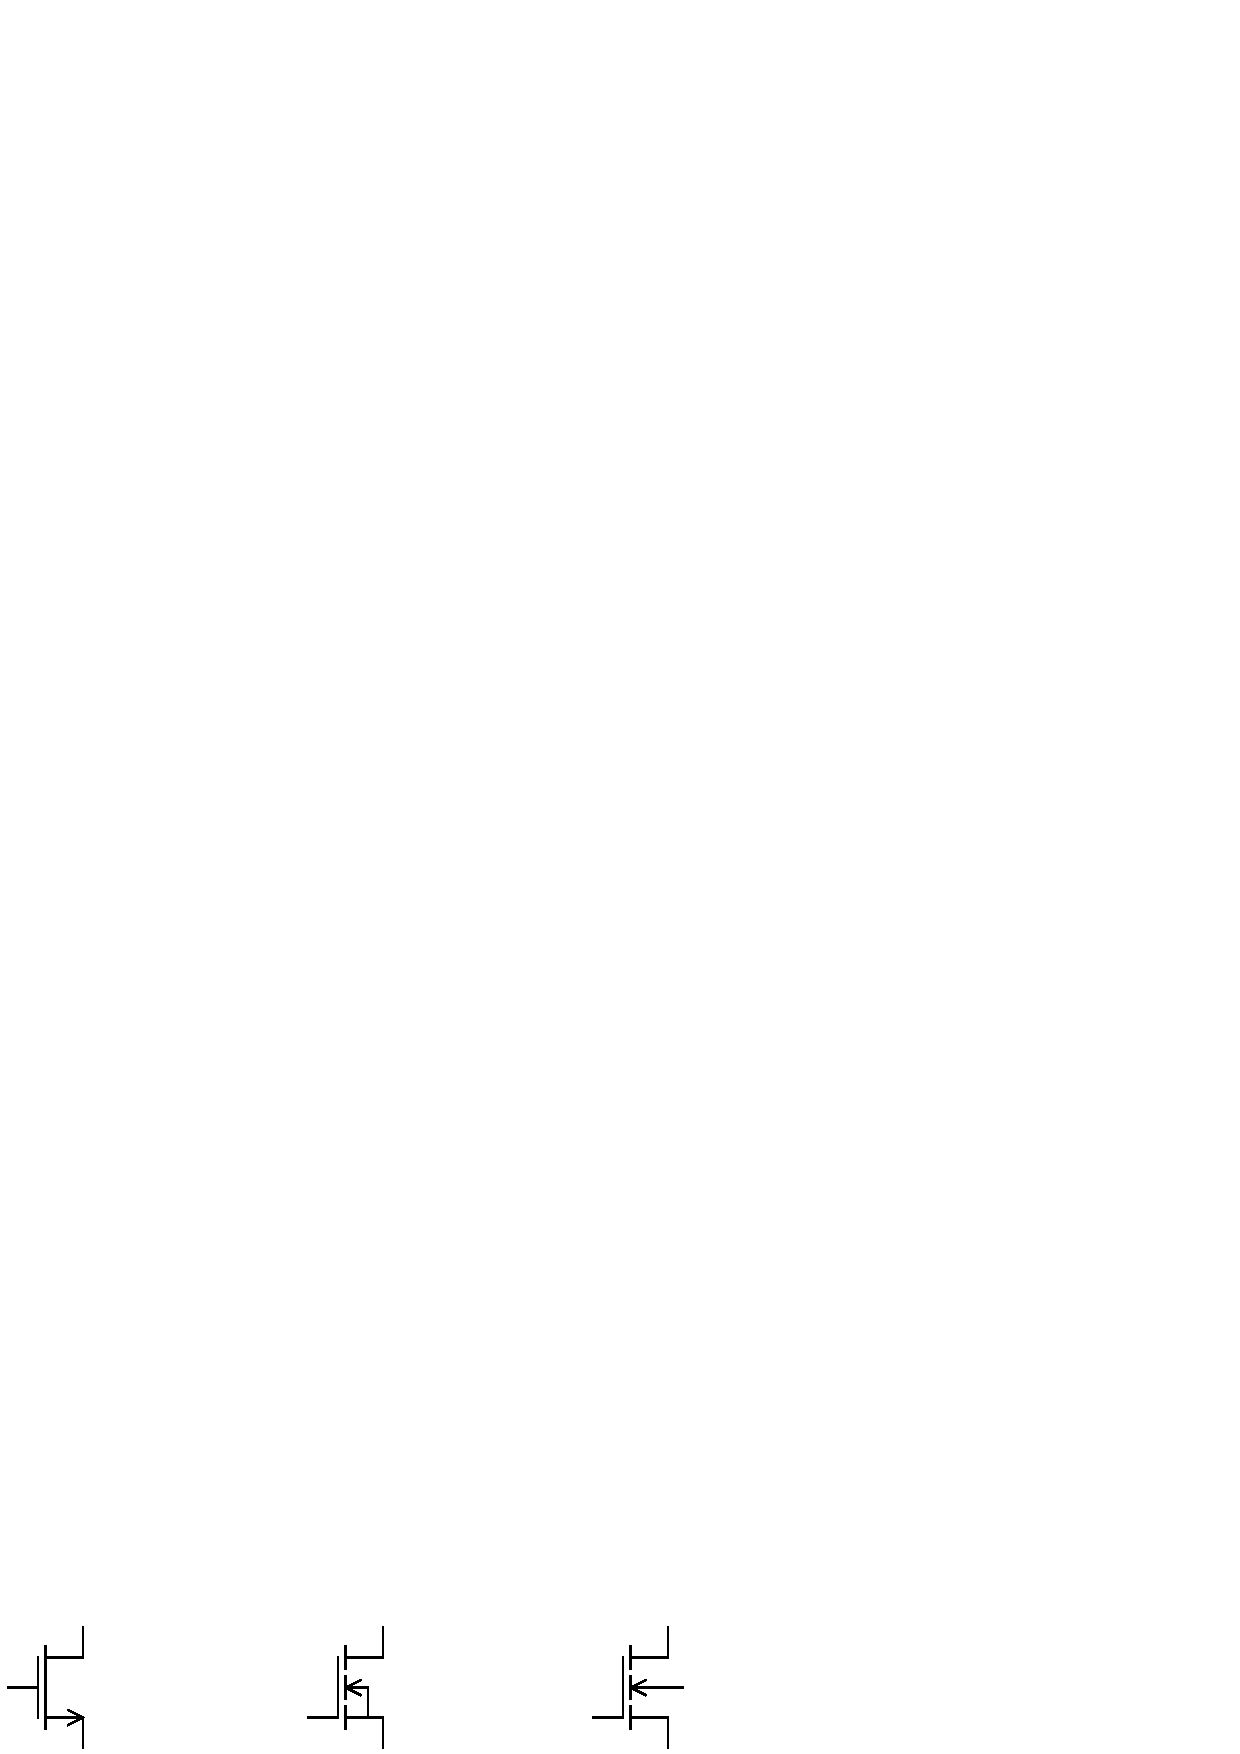
\includegraphics[scale=0.90]{nMosfetEnhancementSymbols}
\caption{\عددی{n} بڑھاتا ماسفیٹ کی مختلف علامتیں}
\label{شکل_منفی_ماسفیٹ_کی_علامتیں}
\end{figure}

جیسا کہ آپ دیکھیں گے گیٹ اور سورس سروں کے مابین \اصطلاح {برقی دباو کی شدت}\حاشیہد{MOSFET کے نام کے پہلے تین مخفف یعنی MOS اس کی ساخت یعنی Semiconductor Oxide Metal سے حاصل کئے گئے ہیں جبکہ بقایا مخفف یعنی FET برقی دباو کی شدت سے چلنے کے عمل یعنی Transistor Effect Field سے لئے گئے ہیں۔}  کے ذریعہ سلیکان کی پتری میں، گیٹ کے نیچے، سورس اور ڈرین خطوں کے مابین برقی رو کے لئے \اصطلاح {راہ}\فرہنگ{راہ}\فرہنگ{channel}\حاشیہب{channel}  پیدا کی جاتی ہے۔اس راہ کے مقام کو شکل  ت میں دکھایا گیا ہے۔سورس اور ڈرین سروں کے مابین برقی دباو لاگو کرنے سے اس راہ میں برقی رو کا گزر ہوتا ہے۔جیسا کہ شکل سے واضح ہے اس راہ کی لمبائی \عددی{L} اور چوڑائی \عددی{W} ہو گی۔راہ کی لمبائی عموماً \عددی{\SI{1}{\micro \meter}}   تا \عددی{\SI{10}{\micro \meter}} جبکہ اس کی چوڑائی \عددی{\SI{2}{\micro \meter}} تا \عددی{\SI{500}{\micro \meter}} ہوتی ہے۔

دو جوڑ ٹرانزسٹر میں بیس پر لاگو برقی رو کی مدد سے ٹرانزسٹر میں برقی رو \عددی{I_C} کو قابو کیا جاتا ہے جہاں بیس میں \عددی{\frac{I_C}{\beta}} برقی رو درکار ہوتی ہے۔اس کے برعکس ماسفیٹ کے گیٹ  اور بقایا حصوں کے درمیان غیر موصل \عددی{\mathrm{SiO_2}} پایا جاتا ہے جس میں برقی رو کا گزر تقریباً ناممکن ہوتا ہے۔حقیقت میں گیٹ میں یک سمتی برقی رو کی مقدار \عددی{10^{-15}} ایمپیئر کے لگ بھگ  ہوتی ہے جو ایک قابلِ نظر انداز مقدار ہے۔

دو جوڑ ٹرانزسٹر کے برعکس میدانی ٹرانزسٹروں میں دونوں \عددی{n+} خطے بالکل یکساں ہوتے ہیں اور ان میں کسی ایک کو بطور سورس اور دوسرے کو ڈرین خطہ استعمال کیا جا سکتا ہے۔ 

اگرچہ موجودہ کئی اقسام کے میدانی ٹرانزسٹروں کے ساخت مندرجہ بالا بتلائے ساخت سے مختلف ہوتے ہیں (جیسے ان میں عموماً دھات کے بجائے دیگر مصنوعی  اجزاء استعمال کئے جاتے ہیں) ہم پھر بھی انہیں ماسفیٹ پکاریں گے۔

\حصہ{\عددی{n} ماسفیٹ کی بنیادی کارکردگی}

\جزوحصہ{گیٹ پر برقی دباو کی عدم موجودگی}
\عددی{n} ماسفیٹ، جسے ہم اس کتاب میں منفی ماسفیٹ بھی کہیں گے، کے گیٹ پر برقی دباو لاگو کئے بغیر اسے دو آپس میں الٹے جڑے ڈایوڈ تصور کیا جا سکتا ہے جہاں \عددی{p} سلیکان پتری (بدن) اور  \عددی{n+} سورس پہلا ڈایوڈ اور اسی طرح \عددی{p}  سلیکان پتری (\اصطلاح {بدن}) اور \عددی{n+}  ڈرین دوسرا ڈایوڈ ہے۔یہ دو الٹے جڑے ڈایوڈ ڈرین اور سورس سروں کے مابین برقی رو کے گزر کو ناممکن بناتے ہیں۔اس صورت میں ان دو سروں کے مابین نہایت زیادہ مزاحمت (تقریباً   \عددی{\SI{e12}{\ohm}}) پائی جاتی ہے۔

شکل \حوالہ{شکل_برقی_راہ_کا_وجود_پیدا_ہونا} الف میں ماسفیٹ کا گیٹ آزاد رکھ کر اس کے سورس اور ڈرین سروں کے مابین برقی دباو \عددی{v_{DS}} لاگو کیا گیا ہے۔مزید یہ کہ ان کے \اصطلاح {بدن} اور ڈرین دونوں سروں کو برقی زمین پر رکھا گیا ہے۔ \عددی{v_{DS}}  لاگو کرنے سے ڈرین-بدن جوڑ پر ویران خطہ بڑھ جاتا ہے اور اس برقی دباو کو روکے رکھتا ہے۔

\جزوحصہ{گیٹ کے ذریعہ برقی رو کے لئے راہ  کی تیاری}
شکل \حوالہ{شکل_برقی_راہ_کا_وجود_پیدا_ہونا} ب میں بدن اور سورس کو برقی زمین پر رکھتے ہوئے گیٹ پر برقی دباو \عددی{v_{GS}} مہیا کیا گیا ہے۔گیٹ پر مثبت برقی دباو  \عددی{p} قسم کی سلیکان پتری میں آزاد خول کو دور دھکیلتا ہے جبکہ یہاں موجود آزاد اقلیتی الیکٹران کو گیٹ کی جانب کھینچتا ہے۔مزید یہ کہ اس برقی دباو کی وجہ سے دونوں \عددی{n+} خطوں میں موجود (ضرورت سے زیادہ تعداد میں) آزاد الیکٹرانوں کو بھی گیٹ کے نیچے کھینچا جاتا ہے۔اگر گیٹ پر مثبت برقی دباو بتدریج بڑھایا جائے تو گیٹ کے نیچے \عددی{p} سلیکان میں الیکٹرانوں کی تعداد بڑھتی ہے اور آخر کار  الیکٹرانوں کی تعداد خولوں کی تعداد سے بھی زیادہ ہو جاتی ہے۔اس عمل سے \عددی{p} خطہ الٹا ہو کر \عددی{n} خطہ بن جاتا ہے۔ایک قسم کے سلیکان سے زبردستی دوسری قسم کی سلیکان بنانے کے عمل کو \اصطلاح {الٹا کرنا}\فرہنگ{الٹا!کرنا}\حاشیہب{inversion}\فرہنگ{inversion} کہتے ہیں اور ایسے الٹا کئے گئے خطے کو  \اصطلاح {الٹا خطہ}\فرہنگ{الٹا!خطہ}\حاشیہب{inversion layer}\فرہنگ{inversion layer} کہا جاتا ہے۔گیٹ پر برقی دباو بڑھانے سے گیٹ کے نیچے \اصطلاح {الٹا خطہ} بھی بڑھتا ہے اور آخر کار یہ سورس سے ڈرین تک پہل جاتا ہے۔یوں سورس سے ڈرین تک \عددی{n} قسم کی راہ وجود میں آتی ہے۔جیسے ہی سورس اور ڈرین خطوں کے مابین راہ پیدا ہوتا ہے ان خطوں کے مابین برقی رو کا گزر ممکن ہو جاتا ہے۔جس برقی دباو پر ایسا ہو جائے اس کو \اصطلاح {دہلیز برقی دباو}\فرہنگ{دہلیز برقی دباو}\فرہنگ{برقی دباو!دہلیز}\فرہنگ{threshold voltage}\حاشیہب{threshold voltage}  \عددی{V_t} کہتے ہیں۔شکل  ب میں یوں پیدا کیا گیا راہ دکھایا گیا ہے۔حقیقت میں \عددی{V_t} سے ذرا سی زیادہ برقی دباو پر برقی رو کا گزر ممکن ہوتا ہے۔یوں ہم کہہ سکتے ہیں کہ گیٹ پر \عددی{V_t} یا اس سے کم برقی دباو کی صورت میں ٹرانزسٹر \اصطلاح {غیر چالو} یا \اصطلاح {منقطع} رہتا ہے جبکہ گیٹ پر \عددی{V_t} سے زیادہ برقی دباو کی صورت میں ٹرانزسٹر \اصطلاح {چالو} یا \اصطلاح {غیر منقطع} رہتا ہے یعنی
\begin{gather}
\begin{aligned}
v_{GS} &\le  V_t && & & \text{منقطع} \\
v_{GS} & > V_t && & & \text{چالو یا غیر منقطع}
\end{aligned}
\end{gather}
یوں \عددی{v_{GS}=V_t} کو \اصطلاح {دہلیز} تصور کیا جا سکتا ہے جس کی ایک جانب ماسفیٹ چالو جبکہ اس کی دوسری جانب ماسفیٹ منقطع رہتا ہے۔چالو ماسفیٹ کے ڈرین اور سورس سروں کے مابین برقی دباو \عددی{v_{DS}} لاگو کرنے سے  \اصطلاح {پیدا کردہ راہ} میں برقی رو \عددی{i_{DS}} گزرے گی۔چونکہ گیٹ کی برقی رو کی قیمت صفر ہے لہٰذا ڈرین سرے پر برقی رو \عددی{i_D} اور سورس سرے پر برقی رو \عددی{i_S} کی قیمتیں برابر ہوں گی یعنی 
\begin{gather}
\begin{aligned}
i_G &=0 \\
i_D &=i_S= i_{DS}
\end{aligned}
\end{gather}
دھیان رہے کہ \عددی{p} قسم کی سلیکان پتری پر \عددی{n} قسم کا راہ پیدا ہوتا ہے اور ایسے ٹرانزسٹر کا پورا نام  \عددی{n}  ماسفیٹ \تحریر{nMOSFET} ہے جہاں \عددی{n} اس \اصطلاح {پیدا کردہ راہ} کے قسم کو بتلاتا ہے۔\عددی{n} راہ میں برقی رو کا وجود الیکٹرانوں کے حرکت کی بدولت ہے جو سورس سے راہ میں داخل ہو کر ڈرین تک سفر کرتے ہیں۔اس کو یوں بھی کہا جا سکتا ہے کہ الیکٹران سورس سے راہ میں خارج ہوتے ہیں اور ڈرین پر راہ سے حاصل کئے جاتے ہیں۔اسی سے ماسفیٹ کے ان دو خطوں کے نام \اصطلاح {سورس}\حاشیہب{source} اور \اصطلاح {ڈرین}\حاشیہب{drain} نکلے\حاشیہد{جس مقام سے کوئی چیز خارج ہو، اُس کو انگریزی میں سورس کہتے ہیں اور جہاں سے نکاسی ہو اس کو ڈرین کہتے ہیں۔} ہیں۔جیسے آپ آگے دیکھیں گے، ماسفیٹ کے گیٹ کی مدد سے ماسفیٹ میں برقی رو کو قابو کیا جاتا ہے۔اسی سے \اصطلاح {گیٹ} کا نام نکلا ہے۔
\begin{figure}
\centering
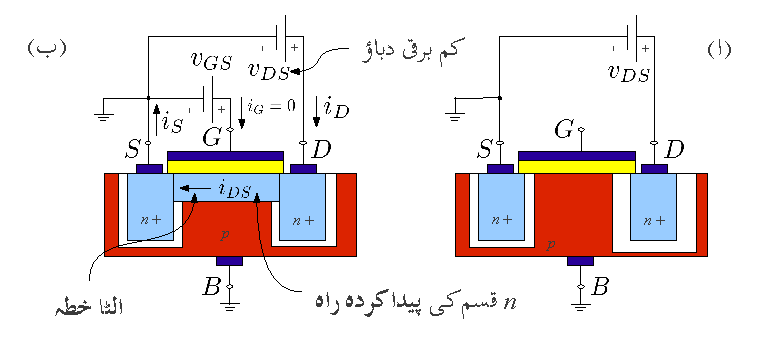
\includegraphics[scale=0.90]{channelCreation}
\caption{برقی راہ کا وجود پیدا ہونا}
\label{شکل_برقی_راہ_کا_وجود_پیدا_ہونا}
\end{figure}
جیسا کہ اوپر ذکر ہوا، \عددی{v_{DS}} لاگو کئے بغیر \عددی{V_t} یا اس سے زیادہ \عددی{v_{GS}} لاگو کرنے  سے \عددی{n} قسم کا راہ پیدا ہوتا ہے۔اس \اصطلاح {پیدا کردہ راہ} کو شکل \حوالہ{شکل_پیدا_کردہ_راہ_کی_مزاحمت} الف میں دکھایا  گیا ہے۔گیٹ پر لاگو برقی دباو کو \عددی{V_t} سے مزید بڑھانے سے گیٹ کے نیچے الیکٹرانوں کی تعداد مزید بڑھتی ہے اور یوں \اصطلاح {پیدا کردہ راہ} کی گہرائی \عددی{g} بڑھتی ہے۔یوں اس قسم کے ماسفیٹ کو \عددی{n} \اصطلاح {بڑھاتا ماسفیٹ}
\فرہنگ{ماسفیٹ!بڑھاتا}\فرہنگ{enhancement nMOSFET}\حاشیہب{enhancement nMOSFET}  کہتے ہیں۔شکل  الف میں \اصطلاح {پیدا کردہ راہ} اور اس کی مزاحمت \عددی{R}  دکھائی گئی ہے جہاں \عددی{n} قسم کے راہ کے \اصطلاح {موصلیت کا مستقل}\حاشیہب{conductivity} \عددی{\sigma} ہے۔
\begin{figure}
\centering
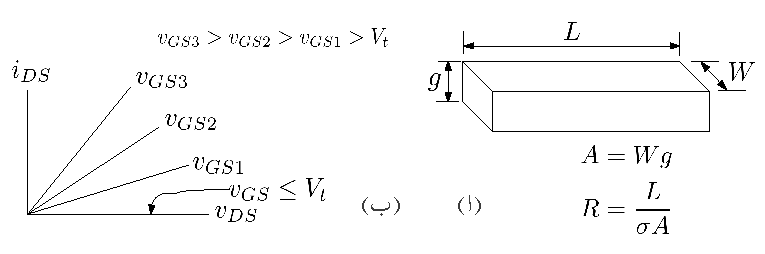
\includegraphics[scale=0.90]{channelResistance}
\caption{پیدا کردہ راہ کی مزاحمت}
\label{شکل_پیدا_کردہ_راہ_کی_مزاحمت}
\end{figure}
گیٹ پر \عددی{v_{GS1}}  برقی دباو (جہاں \عددی{V_{GS1}} کی قیمت  \عددی{V_t} سے زیادہ ہے) سے \اصطلاح {پیدا کردہ راہ} کو مزاحمت \عددی{R} تصور کرتے ہوئے ہم دیکھتے ہیں کہ اس پر لمبائی کی جانب تھوڑا سا برقی دباو \عددی{v_{DS}} لاگو کرنے سے اس میں برقی رو \عددی{i_{DS}} گزرے گی۔شکل \حوالہ{شکل_پیدا_کردہ_راہ_کی_مزاحمت} ب میں انہیں گراف کیا گیا ہے جہاں خط کے قریب لکھ کر اس بات کی یاد دہانی کرائی گئی ہے کہ راہ کو \عددی{V_{GS1}}  برقی دباو سے حاصل کیا گیا ہے۔گیٹ پر برقی دباو \عددی{V_{GS}} بڑھانے سے \اصطلاح {پیدا کردہ راہ} کی گہرائی \عددی{g}  بڑھتی ہے جس سے اس کی مزاحمت \عددی{R}  کم  ہوتی ہے اور یوں \عددی{v_{DS}  -  i_{DS}}  کے گراف کا ڈھلوان بڑھتا ہے۔اس حقیقت کو شکل  ب میں دکھایا گیا ہے جہاں گیٹ پر نسبتاً زیادہ برقی دباو یعنی \عددی{v_{GS2}} لاگو کرتے ہوئے \عددی{v_{DS}  -  i_{DS}} کا خط گراف  کیا گیا ہے۔اسی طرح گیٹ پر برقی دباو کو مزید بڑھا کر \عددی{v_{GS3}} کرتے ہوئے بھی  \عددی{v_{DS}  - i_{DS}} کا خط گراف کیا گیا ہے۔

سورس خطے کو برقی زمین پر رکھتے ہوئے گیٹ پر لاگو برقی دباو جیسے ہی \عددی{V_t} سے تجاوز کر جائے، سورس اور ڈرین خطوں کے درمیان راہ پیدا ہو جاتی ہے۔یوں پیدا کردہ راہ کی گہرائی  \عددی{g} گیٹ پر \عددی{V_t}   سے  اضافی برقی دباو ( \عددی{v_{GS}-V_t} ) پر منحصر ہوتی ہے۔

یاد رہے کہ گیٹ کے نیچے کسی بھی نقطے پر \عددی{p} قسم سلیکان کی پتری میں \عددی{n} قسم کی راہ پیدا کرنے کی خاطر یہ ضروری ہے کہ اس نقطہ پر گیٹ اور سلیکان کی پتری کے مابین کم از کم  \عددی{ V_t} برقی دباو پایا جائے۔اگر گیٹ اور سلیکان پتری کے مابین \عددی{V_t} برقی دباو پایا جائے تو پیدا کردہ راہ کی گہرائی لامحدود کم ہو گی۔پیدا کردہ راہ کی گہرائی گیٹ اور سلیکان پتری کے مابین \عددی{V_t} سے اضافی برقی دباو پر منحصر ہے۔
\begin{figure}
\centering
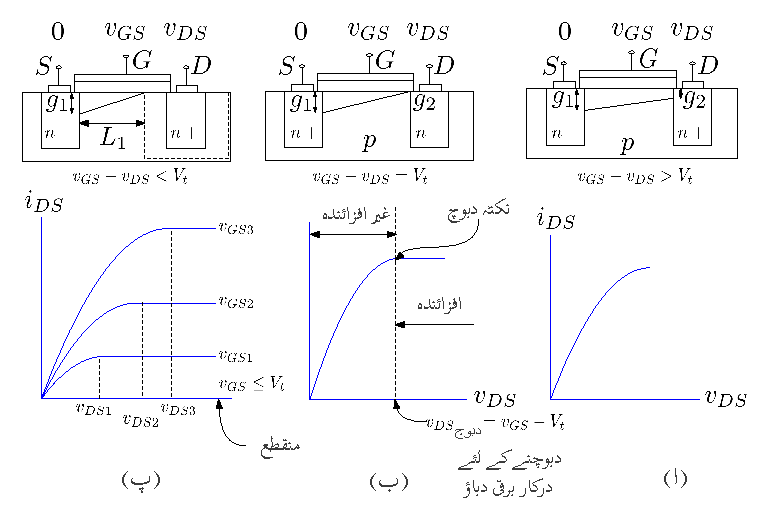
\includegraphics[scale=0.90]{nEnhancementMOSFETcharacteristics}
\caption{پیدا کردہ راہ کی گہرائی اور \عددی{n} بڑھاتے ماسفیٹ کے خط}
\label{شکل_بڑھاتے_ماسفیٹ_کے_خط_منفی}
\end{figure}

شکل \حوالہ{شکل_بڑھاتے_ماسفیٹ_کے_خط_منفی} الف میں سورس خطہ برقی زمین یعنی صفر وولٹ پر ہے جبکہ گیٹ پر \عددی{v_{GS}} برقی دباو ہے۔ یوں یہاں گیٹ اور سلیکان پتری کے مابین \عددی{(v_{GS}-0=v_{GS})}  برقی دباو پایا جاتا ہے اور پیدا کردہ راہ کی گہرائی اضافی برقی دباو یعنی \عددی{(v_{GS}-V_t)} پر منحصر ہو گی جسے شکل میں \عددی{g_1} کہا گیا ہے۔اسی شکل میں ڈرین خطہ \عددی{v_{DS}} وولٹ پر ہے اور یوں یہاں پیدا کردہ راہ کی گہرائی \عددی{(v_{GS}-v_{DS}-V_t)} کے اضافی برقی دباو پر منحصر ہو گی جسے شکل میں \عددی{g_2} کہا گیا ہے۔آپ دیکھ سکتے ہیں کہ \عددی{g_2} کی مقدار \عددی{g_1} سے کم ہے۔یوں پیدا کردہ راہ تکونی شکل اختیار کر لے گا۔ \عددی{v_{DS}} کی مقدار صفر ہونے کی صورت میں \عددی{g_1} اور \عددی{g_2} برابر ہوتے ہیں اور \اصطلاح {پیدا کردہ راہ کی مزاحمت} یعنی  \اصطلاح {چالو ماسفیٹ کی مزاحمت}
\begin{align}\label{مساوات_ماسفیٹ_چالو_ماسفیٹ_کی_مزاحمت}
\textup{مزاحمت}=\frac{\textup{لمبائی}}{\textup{موصلیت کا مستقل} \times \textup{رقبہ}}=\frac{L}{\sigma W g}
\end{align}
 کے برابر ہوتی ہے۔ \عددی{v_{DS}} کی مقدار صفر وولٹ سے بڑھانے سے \عددی{g_2}  کم ہوتا ہے اور پیدا کردہ راہ کی مزاحمت بڑھتی ہے جس سے \عددی{v_{DS} - i_{DS}}  خط کی ڈھلوان کم ہو گی۔شکل  الف میں بڑھتے \عددی{v_{DS}} کے ساتھ \عددی{v_{DS}  - i_{DS}} خط کی ڈھلوان بتدریج کم ہوتی دکھائی گئی ہے۔

آپ دیکھ سکتے ہیں کہ  \عددی{v_{DS}} کو بڑھا کر \عددی{g_2} کی مقدار صفر کی جا سکتی ہے جیسے شکل  ب میں دکھایا گیا ہے۔ہم کہتے ہیں کہ پیدا کردہ راہ \اصطلاح {دبوچ}\فرہنگ{دبوچ}\حاشیہب{pinch off}\فرہنگ{pinch off}  دی گئی ہے۔

سورس خطے کو برقی زمین اور گیٹ کو \عددی{v_{GS}}  برقی دباو پر رکھتے ہوئے اگر \عددی{v_{DS}} بڑھایا جائے تو ڈرین خطے کے بالکل قریب گیٹ اور سلیکان پتری کے مابین \عددی{{v_{GS}-v_{DS}}} برقی دباو پایا جائے گا اور جب تک یہ برقی دباو \عددی{V_t} سے زیادہ رہے یہاں \عددی{n}  قسم کی راہ برقرار رہے گی۔اگر \عددی{v_{GS}-v_{DS}} کی قیمت \عددی{V_t} سے کم ہو تب ڈرین کے قریب راہ کا بننا ممکن نہیں ہو گا۔جب
\begin{align} \label{مساوات_میدانی_منقطع_دباو}
v_{GS}-v_{DS}=V_t
\end{align}
ہو جائے تو ہم کہتے ہیں کہ پیدا کردہ راہ \اصطلاح {دبوچ} دی گئی ہے اور جس \عددی{v_{DS}}  پر ایسا ہو اسے پیدا کردہ راہ \اصطلاح {دبوچنے کے لئے درکار برقی دباو} \زیرنوشت{V}{DS}{دبوچ}  کہتے ہیں۔مساوات \حوالہ{مساوات_میدانی_منقطع_دباو}   سے
\begin{align}\label{مساوات_ماسفیٹ_نقطہ _دبوچ}
V_{\textup{DSدبوچ}}=v_{GS}-V_t
\end{align}
حاصل ہوتا ہے۔مساوات \حوالہ{مساوات_میدانی_منقطع_دباو} میں \عددی{v_{GS}=v_G-v_S} اور \عددی{v_{DS}=v_D-v_S} لکھتے ہوئے
\begin{align*}
\left(v_G-v_S\right) -\left(v_D-v_S \right)&=V_t\\
v_G-v_D&=V_t
\end{align*}
حاصل ہوتا ہے جس میں \عددی{v_{GD}=v_G-v_D} لکھ کر
\begin{align}
v_{\textup{GDدبوچ}}=V_t
\end{align} 
لکھا جا سکتا ہے۔

یہاں ایسا محسوس ہوتا ہے کہ پیدا کردہ راہ کی گہرائی صفر ہوتے ہی (یعنی راہ \اصطلاح {دبوچتے} ہی) راہ کی مزاحمت لامحدود ہو جائے گی اور ٹرانزسٹر میں برقی رو کا گزرنا نا ممکن ہو جائے گا۔حقیقت میں ایسا نہیں ہوتا۔جب تک  \عددی{v_{DS}} کی قیمت \زیرنوشت{v}{DS}{دبوچ} سے کم رہے، اسے بڑھانے سے \عددی{i_{DS}}  بتدریج بڑھتا ہے مگر چونکہ   \عددی{v_{DS}} بڑھانے سے پیدا کردہ راہ کی مزاحمت بھی بڑھتی ہے لہٰذا \عددی{i_{DS}} کے بڑھنے کی شرح بتدریج کم ہوتی ہے۔\زیرنوشت{v}{DS}{دبوچ} پر ٹرانزسٹر میں گزرتی برقی رو کی قیمت \زیرنوشت{i}{DS}{دبوچ} کہلاتی ہے اور اگر \عددی{v_{DS}} کو \زیرنوشت{v}{DS}{دبوچ} سے بڑھایا جائے تو دیکھا جاتا ہے کہ ٹرانزسٹر سے گزرتی برقی رو مستقل \زیرنوشت{i}{DS}{دبوچ} کے برابر ہی رہتی ہے اور اس میں کسی قسم کا اضافہ نہیں آتا۔یہ تمام شکل  ب میں دکھایا گیا ہے۔

شکل \حوالہ{شکل_بڑھاتے_ماسفیٹ_کے_خط_منفی} ب میں ٹرانزسٹر کے  \اصطلاح {افزائندہ} اور \اصطلاح {غیر افزائندہ} خطے بھی دکھائے گئے ہیں۔یہ \اصطلاح {دو جوڑ ٹرانزسٹر} کے نوعیت کے ہی ہیں۔شکل \حوالہ{شکل_بڑھاتے_ماسفیٹ_کے_خط_منفی} پ میں مختلف گیٹ کے برقی دباو پر \عددی{{i_{DS} - v_{DS} }} کے خط کھینچے گئے ہیں اور ان کے \اصطلاح {نقطہ  دبوچ} پر برقی دباو کو \عددی{v_{DS1}} ، \عددی{v_{DS2}} اور \عددی{v_{DS3}} لکھ کر واضح کیا گیا ہے۔سورس خطہ برقی زمین پر رکھتے ہوئے اگر گیٹ پر برقی دباو \عددی{V_t} سے کم ہو تب راہ وجود میں نہیں آتا اور ٹرانزسٹر \اصطلاح {منقطع صورت} اختیار کئے رہتا ہے اور اس میں برقی رو کی قیمت صفر رہتی ہے۔منقطع صورت  بھی اسی شکل میں دکھایا گیا ہے۔

\عددی{n} ماسفیٹ کے ان نتائج کو یہاں ایک جگہ لکھتے ہیں۔
\جزوحصہء{منقطع}
\begin{align}
v_{GS} \le V_t
\end{align}
\جزوحصہء{چالو}
\begin{gather} \label{مساوات_میدانی_کارکردگی_کے_خطے}
\begin{aligned}
v_{GS}-v_{DS} & \ge V_t &&&& \textup{غیر افزائندہ}\\
v_{GS}-v_{\textup{DSدبوچ}} &=V_t &&&& \textup{نقطہ دبوچ}\\
v_{GS}-v_{DS}& \le V_t &&&& \textup{افزائندہ}
\end{aligned}
\end{gather}
انہیں مساوات کو یوں
\begin{gather} \label{مساوات_میدانی_کارکردگی_کے_خطے_الف}
\begin{aligned}
v_{GS} & \le  V_t &&&& \textup{منقطع}\\
v_{DS}& \le v_{GS}-V_t &&&& \textup{غیر افزائندہ}\\
v_{\textup{DSدبوچ}}& = v_{GS}-V_t &&&& \textup{نقطہ دبوچ}\\
v_{DS} & \ge v_{GS}-V_t &&&&\textup{افزائندہ}
\end{aligned}
\end{gather}
یا یوں
\begin{gather}
\begin{aligned}
v_{GS} & \le  V_t &&&& \textup{منقطع}\\
v_{GD}& \ge V_t &&&& \textup{غیر افزائندہ}\\
v_{\textup{GDدبوچ}}& =  V_t &&&& \textup{نقطہ دبوچ}\\
v_{GD} & \le V_t &&&&\textup{افزائندہ}
\end{aligned}
\end{gather}
 بھی لکھا جا سکتا ہے۔یاد رہے کہ \اصطلاح {افزائندہ} یا \اصطلاح {غیر افزائندہ} خطے ہونے کے لئے لازمی ہے کہ ماسفیٹ چالو (یعنی غیر منقطع) ہو۔ماسفیٹ کو \اصطلاح {افزائندہ خطے} میں رکھ کر ایمپلیفائر بنایا جاتا ہے۔  
%===========


\ابتدا{مثال}
شکل \حوالہ{شکل_پیدا_کردہ_راہ_میں_مختلف_مقامات_پر_برقی_دباو} الف میں  \عددی{n} ماسفیٹ کے پیدا کردہ راہ کو بطور سو اُوہم  \عددی{(\SI{100}{\ohm})}  کے موصل  سلاخ دکھایا گیا ہے جس پر لمبائی کے جانب دس وولٹ \عددی{(\SI{10}{\volt})}  برقی دباو لاگو کیا گیا ہے۔مسئلہ کو سادہ رکھنے کی خاطر پیدا کردہ راہ کے ترچھا پن کو نظر انداز کریں۔
\begin{enumerate}
\item
 پیدا کردہ راہ کے مختلف مقامات پر برقی دباو حاصل کریں۔
\item
اگر \عددی{V_t = \SI{3}{\volt}} اور \عددی{v_{GS}=\SI{15}{\volt}} ہوں تب پیدا کردہ راہ کا صورتِ حال کیا ہو گا۔
\item
اگر \عددی{V_t=\SI{3}{\volt}} اور \عددی{v_{GS}=\SI{11}{\volt}} ہوں تب پیدا کردہ راہ کا صورتِ حال کیا ہو گا۔
\end{enumerate}


\begin{figure}
\centering
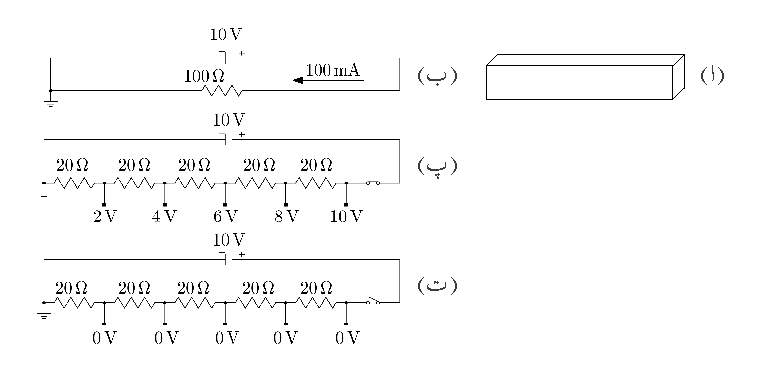
\includegraphics[scale=0.90]{voltageAlongChannel}
\caption{پیدا کردہ راہ میں مختلف مقامات پر برقی دباو}
\label{شکل_پیدا_کردہ_راہ_میں_مختلف_مقامات_پر_برقی_دباو}
\end{figure}
حل:
\begin{enumerate}
\item
موصل سلاخ کو ایک مزاحمت تصور کیا جا سکتا ہے۔یوں اس مسئلہ کو شکل  ب کے طرز پر پیش کیا جا سکتا ہے جس میں \عددی{\SI{100}{\milli \ampere}} برقی رو پیدا ہو گی۔مزید یہ کہ سو اُوہم کے مزاحمت کو کئی مزاحمت سلسلہ وار جڑے تصور کیا جا سکتا ہے۔شکل  پ میں اسے چار عدد \عددی{\SI{20}{\ohm}}  سلسلہ وار جڑے تصور کیا گیا ہے جہاں ہر جوڑ پر برقی دباو بھی دکھایا گیا ہے۔
\item
چونکہ ڈرین سرے پر 
\begin{align*}
v_{GS}-v_{DS}=15-10=5 > V_t
\end{align*}
ہے لہٰذا یہاں پیدا کردہ راہ وجود میں آئے گا اور ٹرانزسٹر میں برقی رو کا گزر ممکن ہو گا۔
\item
 چونکہ ڈرین سرے پر
\begin{align*}
v_{GS}-v_{DS}=11-10=1 < V_t
\end{align*}
ہے لہٰذا پیدا کردہ راہ \اصطلاح {دبوچا} جائے گا۔اگر ایسا ہونے سے \اصطلاح {پیدا کردہ راہ} کی مزاحمت لامحدود ہو جائے اور اس میں برقی رو کی مقدار صفر ہو جائے تو صورتِ حال شکل  ت کے مانند ہو گی جہاں ڈرین سرے پر لامحدود مزاحمت کو بطور منقطع کئے گئے برقی سوئچ دکھایا گیا ہے۔آپ دیکھ سکتے ہیں کہ برقی رو کی عدم موجودگی میں پیدا کردہ راہ میں ہر مقام پر برقی دباو کی مقدار صفر وولٹ \عددی{(\SI{0}{\volt})}  ہو جائے گی اور یوں ڈرین سرے پر بھی صفر وولٹ ہوں جس سے
\begin{align*}
v_{GS}-v_{DS}=11-0=11> V_t
\end{align*}
ہو گا اور یوں برقی رو کا گزر ممکن ہو گا۔

مندرجہ بالا دو نتائج متضاد ہیں۔پہلے نتیجے کے مطابق برقی رو کا گزر نا ممکن ہے جبکہ دوسرے نتیجے کے مطابق، اس کے برعکس، برقی رو کا گزر ممکن ہے۔حقیقی صورتِ حال کو شکل \حوالہ{شکل_بڑھاتے_ماسفیٹ_کے_خط_منفی} پ میں دکھایا گیا ہے جہاں آپ دیکھ سکتے ہیں کہ \اصطلاح {پیدا کردہ راہ} کے \اصطلاح {دبوچنے} کا مقام تبدیل ہو چکا ہے اور یوں پیدا کردہ راہ کی لمبائی قدرِ کم ہو گئی ہے اور ساتھ ہی ساتھ ڈرین سرے پر ویران خطہ اتنا بڑھ گیا ہے کہ ایک جانب یہ ڈرین خطے کو اور دوسری جانب پیدا کردہ راہ کو چھوتا ہے۔چونکہ نقطہ دبوچ پر گیٹ اور پیدا کردہ راہ کے مابین \عددی{V_t}برقی دباو پایا جاتا ہے لہٰذا  \اصطلاح {نقطہ دبوچ} پر
\begin{align*}
v_{\textup{DSدبوچ}}=v_{GS}-V_t
\end{align*}
ہو گا اور ڈرین-سورس سروں کے مابین اضافی برقی دباو \عددی{{(v_{DS}-v_{\textup{DSدبوچ}})}}  ویران خطہ برداشت کرے گا۔

پیدا کردہ راہ پر لاگو برقی دباو \عددی{(v_{\textup{DSدبوچ}})} اس میں برقی رو پیدا کرے گا جو کہ سورس سے ڈرین جانب الیکٹران کے بہاو سے پیدا ہو گا۔یہ الیکٹران \اصطلاح {نقطہ دبوچ} پر پہنچتے ہی ویران خطے میں داخل ہوں گے۔ویران خطے میں آزاد الیکٹران نہیں ٹھر سکتے اور انہیں ڈرین خطے میں  دھکیل دیا جاتا ہے۔یوں الیکٹران سورس سرے سے رواں ہو کر ڈرین سرے پہنچ کر \عددی{i_{DS}}  پیدا کرتے ہیں۔ 

شکل  پ میں گیٹ پر مختلف برقی دباو کے لئے ماسفیٹ کے خط گراف کئے گئے ہیں۔ 

\end{enumerate}
\انتہا{مثال}

%========
\حصہ{\عددی{n} ماسفیٹ کی مساوات}

مندرجہ بالا تذکرے کو مدِ نظر رکھتے ہوئے \عددی{n} ماسفیٹ کی  \عددی{{i_{DS}-v_{DS}}} مساوات حاصل کرتے ہیں۔ایسا کرتے وقت سورس سرے کو برقی زمین (یعنی صفر وولٹ) پر رکھا جائے گا جبکہ گیٹ کو \عددی{v_{GS}}  اور ڈرین سرے کو  \عددی{v_{DS}}  پر رکھا جائے گا۔مزید یہ کہ \عددی{{v_{GS}-v_{DS}> V_t}} رکھا گیا ہے۔

پیدا کردہ راہ میں سورس سے ڈرین خطے کی جانب فاصلے کو \عددی{x} لیتے ہوئے سورس جانب \عددی{x=0} اور برقی دباو صفر وولٹ ہو گا جبکہ ڈرین جانب \عددی{x=L} اور برقی دباو \عددی{v_{DS}}  ہو گا۔ان دو حدود کے درمیان کسی بھی نقطہ  \عددی{x} پر برقی دباو کو ہم \عددی{v(x)} لکھتے ہیں۔
\begin{figure}
\centering
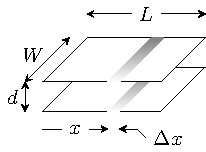
\includegraphics{figMOSFETcapacitor}
\caption{گیٹ اور راہ بطور دو چادر کپیسٹر کردار ادا کرتے ہیں۔}
\label{شکل_ماسفیٹ_گیٹ_راہ_کپیسٹر}
\end{figure}
گیٹ اور پیدا کردہ راہ (یعنی \عددی{n} قسم کا موصل) بطور دو چادر کے \اصطلاح {کپیسٹر}\حاشیہب{parallel plate capacitor}  کا کردار ادا کریں گے۔پیدا کردہ راہ میں لمبائی کے رُخ نقطہ \عددی{x}  پر ذرہ سی لمبائی \عددی{\Delta x} پر غور کرتے ہیں۔یہ لمبائی بطور  کپیسٹنس \عددی{\Delta C} کردار ادا کرے گا جہاں
\begin{align}
\Delta C=\frac{\epsilon \times \textup{رقبہ}}{\textup{فاصلہ}}=\frac{\epsilon  W \Delta x}{d}
\end{align}
ہو گا۔اس کپیسٹر کو شکل \حوالہ{شکل_ماسفیٹ_گیٹ_راہ_کپیسٹر} میں دکھایا گیا ہے۔

آپ کپیسٹر کی مساوات \عددی{Q=C \times V} سے بخوبی آگاہ ہوں گے۔اس مساوات کے مطابق کپیسٹر کے مثبت چادر پر بار  \عددی{Q}  کی مقدار  کپیسٹر کے دو چادروں کے مابین برقی دباو \عددی{V}  پر منحصر ہوتا ہے۔کپیسٹر کے منفی چادر پر \عددی{(-Q)}   بار پایا جاتا ہے۔ماسفیٹ کے کپیسٹر \عددی{\Delta C}  پر بھی  اسی طرح بار پایا جائے گا مگر اس کا تخمینہ لگانے کی خاطر اس مسئلہ کو زیادہ گہرائی سے دیکھنا ہو گا۔آئیں ایسا ہی کرتے ہیں۔

جیسا کہ آپ جانتے ہیں کہ کسی بھی نقطہ \عددی{x}  پر تب راہ پیدا ہوتا ہے جب اس نقطہ پر گیٹ اور سلیکان پتری کے مابین \عددی{V_t} برقی دباو پایا جائے (یعنی جب  \عددی{{v_{GS}-v(x)=V_t}} ہو) اور ایسی صورت میں پیدا کردہ راہ میں قابلِ نظر انداز (تقریباً صفر) مقدار میں \عددی{n} قسم کا بار یعنی آزاد الیکٹران جمع ہوتے ہیں ۔یوں \عددی{{(v_{GS}-V_t-v(x)=0)}} ہونے کی صورت میں آزاد الیکٹرانوں کی تعداد بھی (تقریباً) صفر ہوتی ہے۔جیسے جیسے گیٹ اور سلیکان پتری کے مابین برقی دباو مزید بڑھایا جائے یہاں آزاد الیکٹرانوں کی تعداد بڑھتی ہے۔یوں آزاد الیکٹرانوں کی تعداد کا دارومدار برقی دباو \عددی{{(v_{GS}-V_t-v(x))}} پر ہوتا ہے اور ہم ماسفیٹ کے گیٹ کے لئے کپیسٹر کی مساوات یوں لکھ سکتے ہیں۔
\begin{gather}
\begin{aligned}
\Delta Q&=\Delta C \times V\\
&=\left[\frac{\epsilon W \Delta x}{d} \right ] \times \left[v_{GS}-V_t-v(x) \right ]
\end{aligned}
\end{gather}
پیدا کردہ راہ میں اس نقطہ پر بار کی مقدار اتنی ہی مگر منفی قسم کی ہو گی۔اس مساوات کو پیدا کردہ راہ کے لئے یوں لکھا جا سکتا ہے۔
\begin{align} \label{مساوات_میدانی_راہ_میں_چارج_بالمقابل_فاصلہ}
\frac{\Delta Q_n}{\Delta x}&=-\left[\frac{\epsilon W}{d} \right ] \times \left [v_{GS}-V_t-v(x) \right ]
\end{align}
فاصلہ کے ساتھ برقی دباو کی شرح  کو شدتِ برقی دباو \عددی{E}  کہتے ہیں۔یوں نقطہ  \عددی{x} پر
\begin{align}
E=-\frac{\Delta v(x)}{\Delta x}
\end{align}
ہو گا۔اس کی سمت ڈرین سے سورس خطے کی جانب ہے۔شدتِ برقی دباو کسی بھی مثبت بار کو \عددی{E} کی سمت میں جبکہ منفی بار کو الٹی جانب دھکیلتا ہے۔چونکہ پیدا کردہ راہ میں منفی بار پائے جاتے ہیں لہٰذا شدتِ برقی دباو انہیں سورس سے ڈرین خطے کی جانب دھکیلے گا۔کسی بھی موصل میں چارجوں کی رفتار وہاں کے شدتِ برقی دباو کے برائے راست متناسب ہوتا ہے۔یوں منفی چارجوں کے رفتار کو \عددی{(-\mu_n E)} اور مثبت چارجوں کے رفتار کو  \عددی{(\mu_p E)} لکھا جائے گا جہاں \عددی{\mu_n}  سلیکان پتری میں \اصطلاح {الیکٹران کی حرکت پذیری}\فرہنگ{حرکت پذیری!الیکٹران}\فرہنگ{electron mobility}\حاشیہب{electron mobility}  کہلاتا ہے جبکہ  \عددی{\mu_p} سلیکان پتری میں \اصطلاح {خول کی حرکت پذیری}\فرہنگ{حرکت پذیری!خول}\فرہنگ{hole mobility}\حاشیہب{hole mobility}  کہلاتا ہے۔یہاں \اصطلاح {حرکت پذیری} سے مراد \اصطلاح {الٹا خطے} میں \اصطلاح {حرکت پذیری} ہے۔یہاں رک کر تسلی کر لیں کہ یہ دو مساوات دونوں اقسام کے چارجوں کے رفتار کے صحیح سمت دیتے ہیں۔یوں رفتار کو \عددی{\frac{\Delta x}{\Delta t}} لکھتے ہوئے الیکٹرانوں کے لئے ہم یوں لکھ سکتے ہیں۔
\begin{align} \label{مساوات_میدانی_الیکٹران_کی_رفتار}
\frac{\Delta x}{\Delta t}=-\mu_n E=\mu_n \frac{\Delta v(x)}{\Delta t}
\end{align}
مساوات \حوالہ{مساوات_میدانی_راہ_میں_چارج_بالمقابل_فاصلہ}  اور مساوات \حوالہ{مساوات_میدانی_الیکٹران_کی_رفتار}  کی مدد سے ہم پیدا کردہ راہ میں آزاد الیکٹرانوں کے حرکت سے پیدا برقی رو یوں حاصل کر سکتے ہیں۔
\begin{gather}
\begin{aligned}
i(x)&=\frac{\Delta Q_n}{\Delta t}=\frac{\Delta Q_n}{\Delta x} \times \frac{\Delta x}{\Delta t}\\
&=-\left[\frac{\epsilon W}{d} \right ] \left[v_{GS}-V_t-v(x) \right ] \times \left [\mu_n \frac{\Delta v(x)}{\Delta x} \right ]
\end{aligned}
\end{gather}
اس مساوات کو یوں لکھا جا سکتا ہے۔
\begin{align}
i(x) \Delta x=-\left[\frac{\epsilon W}{d} \right ] \left[v_{GS}-V_t -v(x) \right] \times \left[\mu_n \Delta v(x) \right ]
\end{align}
اس مساوات میں \عددی{\Delta} کو باریک سے باریک تر لیتے ہوئے مساوات کا تکملہ لیتے ہیں جہاں پیدا کردہ راہ کے سورس سرے کو ابتدائی نقطہ جبکہ اس کے ڈرین سرے کو اختتامی نقطہ لیتے ہیں۔یوں ابتدائی نقطہ پر \عددی{x=0}   جبکہ اختتامی نقطہ پر  \عددی{x=L} ہے۔اسی طرح ابتدائی برقی دباو  \عددی{v(0)=0} جبکہ اختتامی برقی دباو  \عددی{v(L)=v_{DS}} ہے۔یوں
\begin{align}
\int_0^{L} {i(x)} \textup{d}x=\int_0^{v_{DS}}-\left[\frac{\epsilon \mu_n W}{d} \right ] \left[v_{GS}-V_t-v(x) \right ] \textup{d}v(x)
\end{align}
چونکہ پیدا کردہ راہ میں از خود برقی رو نہ پیدا اور نہ ہی غائب ہو سکتی ہے لہٰذا اس میں لمبائی کی جانب برقی رو تبدیل نہ ہو گی۔اس برقی رو کو \عددی{i} لکھتے ہوئے تکملہ سے باہر نکالا جا سکتا ہے۔
\begin{gather}
\begin{aligned}
\int_0^{L} {i(x) \textup{d}x}&=i \int_0^{L} {\textup{d}x}=\int_0^{v_{DS}}-\left[\frac{\epsilon \mu_n W}{d} \right ] \left[v_{GS}-V_t-v(x) \right ] \textup{d}v(x)\\
\left. ix \right |_0^{L}&=-\left[\frac{\epsilon \mu_n W}{d} \right ] \left [ \left . \left ( v_{GS} -V_t \right )v(x) \right |_0^{v_{DS}} -\left . \frac{v(x)^2}{2}  \right |_0^{v_{DS}}\right ]
\\
iL&=-\left[\frac{\epsilon \mu_n W}{d} \right ] \left[\left(v_{GS}-V_t \right ) v_{DS}-\frac{v_{DS}^{2}}{2} \right ]\\
i&=-\left[\frac{\epsilon \mu_n}{d} \right ] \left[\frac{W}{L} \right ] \left[ \left(v_{GS}-V_t \right ) v_{DS}-\frac{v_{DS}^{2}}{2}\right ]
\end{aligned}
\end{gather}
منفی برقی رو کا مطلب ہے کہ یہ بڑھتے \عددی{x} کے الٹ جانب رواں ہے یعنی ڈرین سے سورس جانب۔ماسفیٹ میں اسی جانب برقی رو کو \عددی{i_{DS}} لکھا جاتا ہے۔یوں
\begin{align}
i_{DS}=\left[ \frac{\epsilon \mu_n}{d}\right ] \left[  \frac{W}{L}\right ] \left[\left (v_{GS}-V_t \right )v_{DS}-\frac{v_{DS}^{2}}{2} \right ]
\end{align}
نقطہ  دبوچ پر \عددی{v_{\textup{DSدبوچ}}=v_{GS}-V_t} استعمال کرتے اس مساوات سے حاصل ہوتا ہے۔
\begin{gather}
\begin{aligned}
i_{\textup{DSدبوچ}}&=\left[\frac{\epsilon \mu_n}{d} \right ] \left[\frac{W}{L} \right ] \left[ \left(v_{GS}-V_t \right )v_{\textup{DSدبوچ}} - \frac{v_{\textup{DSدبوچ}}^{2}}{2} \right] \\
&=\left[\frac{\epsilon \mu_n}{d} \right ] \left[\frac{W}{L} \right ] \left[ \left(v_{GS}-V_t \right ) \left(v_{GS}-V_t \right ) - \frac{\left(v_{GS}-V_t \right )^{2}}{2} \right] \\
&=\frac{1}{2} \left[\frac{\epsilon \mu_n}{d} \right ] \left[\frac{W}{L} \right ] \left(v_{GS}-V_t \right )^2
\end{aligned}
\end{gather}
چونکہ افزائندہ خطے میں نقطہ دبوچ پر برقی رو کے برابر برقی رو ہی رہتی ہے لہٰذا افزائندہ خطے میں برقی رو کی بھی یہی مساوات ہے۔

ان مساوات میں
\begin{gather}
\begin{aligned}
k_n'&=\left(\frac{\epsilon \mu_n}{d} \right )\\
k_n&=\left(\frac{\epsilon \mu_n}{d} \right ) \left(\frac{W}{L} \right )=k_n' \left(\frac{W}{L} \right )
\end{aligned}
\end{gather}
لیتے ہوئے انہیں دوبارہ لکھتے ہیں۔ساتھ ہی ساتھ ان کا دائرہ عمل متعین کرنے کے نکات بھی درج کرتے ہیں۔

غیر افزائندہ خطہ:
\begin{gather}
\begin{aligned}\label{مساوات_میدانی_غیر_افزائندہ_خطے_کی_نشاندہی}
v_{GS}& > V_t \\
v_{GS}-v_{DS}&= v_{GD}=\ge V_t
\end{aligned}
\end{gather}

\begin{gather} \label{مساوات_میدانی_غیر_افزائندہ_رو}
\begin{aligned}
i_{DS}&=k_n' \left[\frac{W}{L} \right ] \left[\left(v_{GS}-V_t \right )v_{DS}-\frac{v_{DS}^{2}}{2} \right ] \\
&=k_n \left[\left(v_{GS}-V_t \right )v_{DS}-\frac{v_{DS}^{2}}{2} \right ]
\end{aligned}
\end{gather}
نقطہ  دبوچ:
\begin{gather}\label{مساوات_ماسفیٹ_منفی_بڑھاتا_نقطہ _دبوچ}
\begin{aligned}
v_{GS}& > V_t\\
v_{GS}-v_{DSدبوچ}&= v_{GDدبوچ}=V_t
\end{aligned}
\end{gather}

\begin{gather} \label{مساوات_میدانی_نقطہ _دبوچ_رو}
\begin{aligned}
i_{DS}&=\frac{k_n'}{2} \left[\frac{W}{L} \right ] \left[v_{GS}-V_t \right]^{2} \\
&=\frac{k_n}{2} \left[v_{GS}-V_t \right]^{2}
\end{aligned}
\end{gather}
افزائندہ:
\begin{gather}
\begin{aligned}\label{مساوات_میدانی_افزائندہ_خطے_کی_نشاندہی}
v_{GS} > V_t\\
v_{GS}-v_{DS} &=v_{GD} \le V_t 
\end{aligned}
\end{gather}

\begin{gather} \label{مساوات_میدانی_افزائندہ_رو}
\begin{aligned}
i_{DS}&=\frac{k_n'}{2} \left[\frac{W}{L} \right ] \left[v_{GS}-V_t \right]^{2}\\
&=\frac{k_n}{2} \left[v_{GS}-V_t \right]^{2}
\end{aligned}
\end{gather}
منقطع:
\begin{gather}
\begin{aligned}
v_{GS}& \le V_t\\
i_{DS}&=0
\end{aligned}
\end{gather}

ماسفیٹ تخلیق دیتے وقت پیدا کردہ راہ کے چوڑائی \عددی{W}  اور لمبائی \عددی{L} کی تناسب بدل کر مختلف \عددی{i_{DS}-v_{DS}} خط حاصل کئے جاتے ہیں۔

یاد دہانی کی خاطر کچھ باتیں دوبارہ دہراتے ہیں۔
	
\تحریر{nMOSFET}  کو غیر افزائندہ خطے میں استعمال کرنے کی خاطر گیٹ اور سورس کے مابین \عددی{V_t}  سے زیادہ برقی دباو مہیا کیا جاتا ہے اور ڈرین-سورس سروں کے مابین برقی دباو کو راہ دبوچ برقی دباو \زیرنوشت{v}{DS}{دبوچ} سے کم رکھا جاتا ہے یعنی
\begin{gather}
\begin{aligned}
v_{GS} & > V_t &&&& \textup{راہ پیدا}\\
v_{DS}&  \le v_{\textup{DSدبوچ}}  &&&& \textup{نقطہ دبوچ}\\
& \le v_{GS}-V_t
\end{aligned}
\end{gather}
اسی طرح \تحریر{nMOSFET}  کو افزائندہ خطے میں استعمال کرنے کی خاطر گیٹ اور سورس کے مابین \عددی{V_t} سے زیادہ برقی دباو  مہیا کیا جاتا ہے اور ڈرین-سورس سروں کے مابین برقی دباو کو راہ دبوچ برقی دباو \زیرنوشت{v}{DS}{دبوچ}  سے زیادہ رکھا جاتا ہے یعنی
\begin{gather}
\begin{aligned}
v_{GS}& > V_t &&&& \textup{راہ پیدا}\\
v_{DS}& \ge v_{\textup{DSدبوچ}} &&&& \textup{نقطہ دبوچ}\\
& \ge v_{GS}-V_t
\end{aligned}
\end{gather}
نقطہ  دبوچ ان دو خطوں کے درمیان حد ہے جسے دونوں کا حصہ تصور کیا جا سکتا ہے۔

\تحریر{nMOSFET} کو منقطع کرنے کی خاطر گیٹ اور سورس کے مابین \عددی{V_t} یا اس سے  کم برقی دباو رکھا جاتا ہے یعنی
\begin{align}
v_{GS} \le  V_t &&&& \textup{منقطع}
\end{align}
غیر افزائندہ ماسفیٹ پر جب باریک \عددی{v_{DS}} لاگو کیا جائے تو مساوات \حوالہ{مساوات_میدانی_غیر_افزائندہ_رو}  میں \عددی{v_{DS}^2}  کو نظر انداز کرنا ممکن ہوتا ہے اور اس مساوات کو یوں لکھا جا سکتا ہے۔
\begin{align*}
i_{DS}=k_n' \left[\frac{W}{L} \right ]\left[\left(v_{GS}-V_t \right ) v_{DS}-\frac{v_{DS}^{2}}{2} \right ] \approx k_n' \left[\frac{W}{L} \right ]\left[\left(v_{GS}-V_t \right ) v_{DS} \right ]
\end{align*}
اس مساوات سے باریک \عددی{v_{DS}} کی صورت میں ماسفیٹ کی مزاحمت حاصل کی جا سکتی ہے یعنی
\begin{align}
R=\frac{v_{DS}}{i_{DS}}=\frac{1}{k_n' \left[\frac{W}{L} \right ] \left[v_{GS}-V_t \right ]}
\end{align}
ماسفیٹ کے گیٹ پر برقی دباو تبدیل کر کے اس کی مزاحمت تبدیل کی جاتی ہے اور یوں ماسفیٹ کو بطور قابو مزاحمت استعمال کیا جا سکتا ہے۔

شکل \حوالہ{شکل_ماسفیٹ_سادہ_خط} میں ماسفیٹ کا خط دکھایا گیا ہے جس میں افزائندہ اور غیر افزائندہ خطوں کے درمیان لکیر کھینچی گئی ہے۔چونکہ ماسفیٹ غیر افزائندہ سے افزائندہ خطے میں اس وقت داخل ہوتا ہے جب \عددی{v_{GS}-v_{DS}=V_t} یعنی \عددی{v_{GS}-V_t=v_{DS}} ہو لہٰذا مساوات \حوالہ{مساوات_میدانی_افزائندہ_رو} میں \عددی{\left(v_{GS}-V_t \right)} کی جگہ \عددی{v_{DS}} پُر کرنے سے اس لکیر کی مساوات حاصل ہو گی۔یوں 
\begin{align}\label{مساوات_ماسفیٹ_نقطہ _دبوچ_پر_برقی_رو}
i_{DS}=\frac{k_n}{2} v_{DS}^2
\end{align}
حاصل ہوتا ہے جسے شکل \حوالہ{شکل_ماسفیٹ_سادہ_خط} میں ماسفیٹ کے خطوط پر کھینچا گیا ہے جبکہ مساوات \حوالہ{مساوات_میدانی_افزائندہ_رو} کو شکل \حوالہ{شکل_ماسفیٹ_دبوچ} میں کھینچا گیا ہے۔باب \حوالہ{باب_دو_جوڑ_ٹرانزسٹر} میں \اصطلاح {دو جوڑ ٹرانزسٹر} کے غیر افزائندہ اور افزائندہ خطے دکھائے گئے ہیں۔ان کا ماسفیٹ کے خطوں کے ساتھ موازنہ کریں۔ٹرانزسٹر تقریباً \عددی{\SI{0.2}{\volt}} سے کم \عددی{v_{CE}} پر غیر افزائندہ جبکہ اس سے زیادہ برقی دباو پر افزائندہ ہوتا ہے۔ماسفیٹ \عددی{v_{DS \textrm{دبوچ}}} سے کم برقی دباو پر غیر افزائندہ جبکہ اس سے زیادہ برقی دباو پر افزائندہ ہوتا ہے جہاں \عددی{v_{DS \textrm{دبوچ}}} کی قیمت مساوات \حوالہ{مساوات_ماسفیٹ_نقطہ _دبوچ} سے حاصل کی جاتی ہے۔
شکل \حوالہ{شکل_ماسفیٹ_سادہ_خط} اور  \حوالہ{شکل_ماسفیٹ_دبوچ} میں \عددی{k_n=\SI{0.2}{\milli \ampere \per \volt \squared}} اور \عددی{V_t=\SI{1}{\volt}} ہیں۔

%
\begin{figure}
\centering
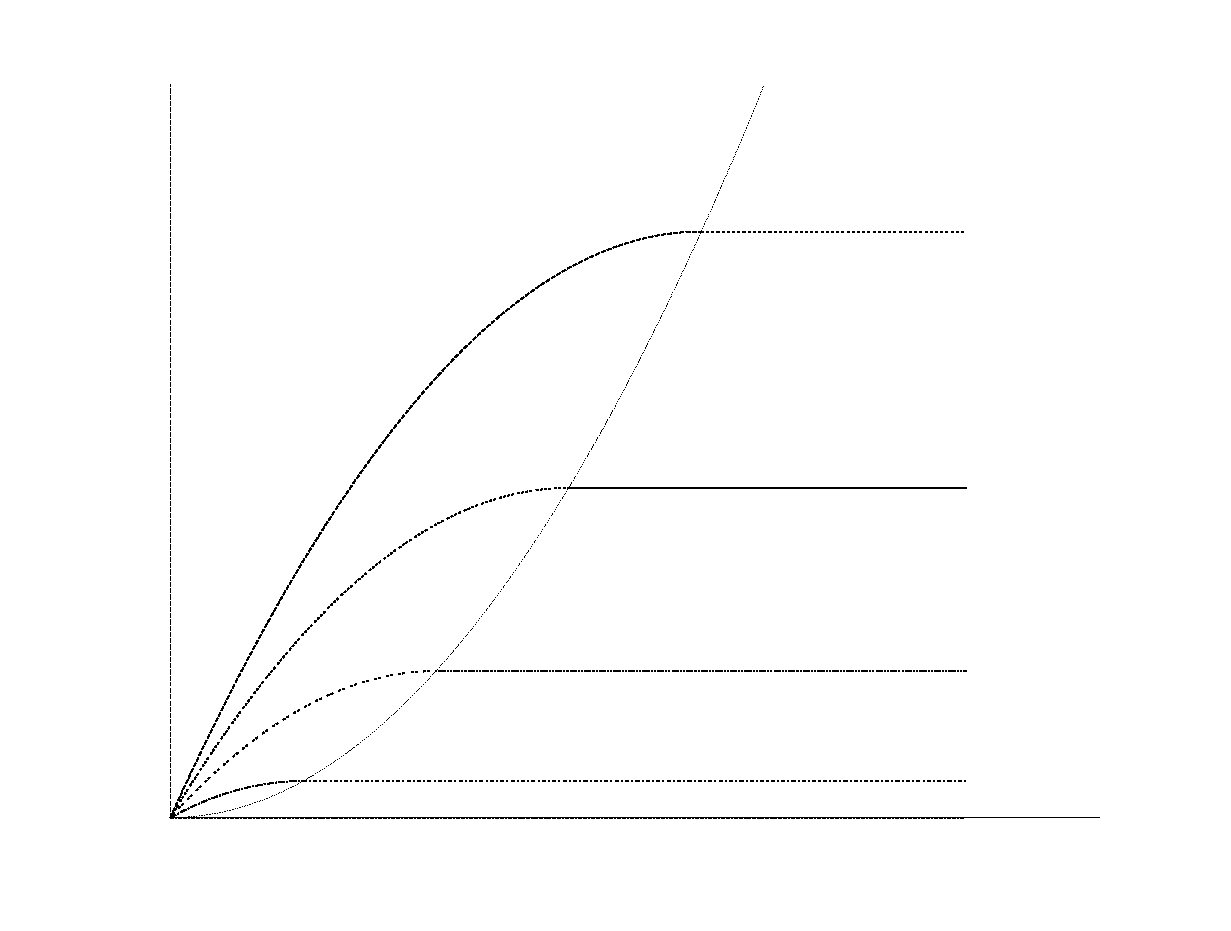
\includegraphics[scale=0.90]{nMOSFETenhancementNormalCharacteristics}
\caption{}
\label{شکل_ماسفیٹ_سادہ_خط}
\end{figure}
%
\begin{figure}
\centering
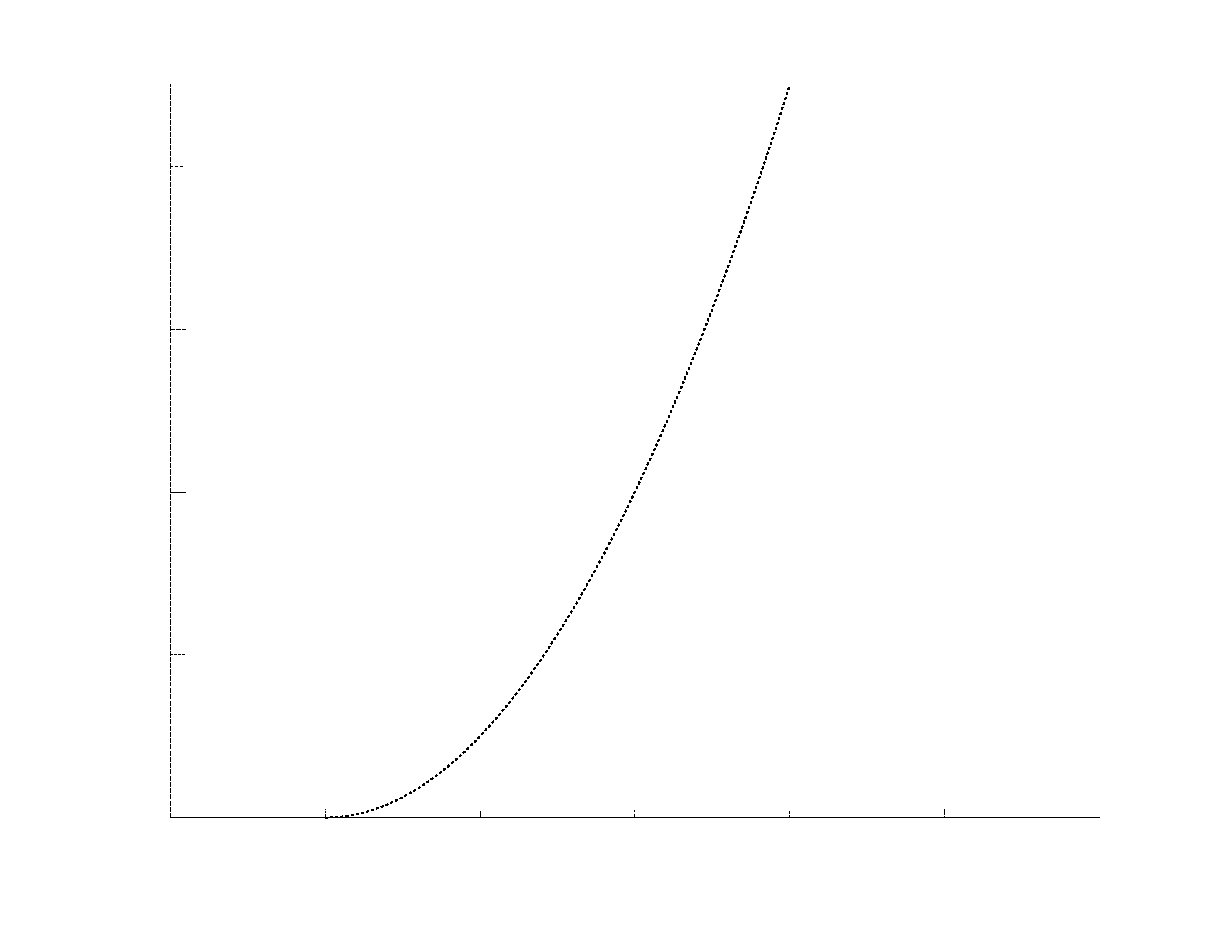
\includegraphics[scale=0.90]{nMOSFETenhancementPinchoff}
\caption{افزائندہ ماسفیٹ کا برقی رو بالمقابل گیٹ کی برقی دباو}
\label{شکل_ماسفیٹ_دبوچ}
\end{figure}

ٹرانزسٹر کے \عددی{\beta} کی طرح ایک ہی قسم کے دو عدد ماسفیٹ کے \عددی{k_n} میں فرق پایا جاتا ہے۔اسی طرح ان کے  \عددی{V_t} میں بھی فرق پایا جاتا ہے۔ان وجوہات کی بنا پر کسی بھی دور میں ماسفیٹ تبدیل کرنے سے نقطہ کارکردگی تبدیل ہونے کا امکان ہوتا ہے۔

\جزوحصہ{قابل برداشت برقی دباو}
\عددی{v_{DS}} کو \زیرنوشت{}{DS}{دبوچ}  سے جتنا بڑھایا جائے، نقطہ دبوچ ڈرین خطے سے اتنا ہی دور ہو جاتا ہے۔اگر اس برقی دباو کو بتدریج بڑھایا جائے تو نقطہ دبوچ آخر کار سورس خطے تک پہنچ جاتا ہے اور ان خطوں کے مابین برقی رو تیزی سے بڑھتا ہے۔یہ عمل تقریباً \عددی{\SI{20}{\volt}} پر پیدا ہوتا ہے۔یہ عمل از خود نقصان دہ نہیں جب تک بے قابو برقی رو ماسفیٹ کی قابلِ برداشت برقی رو کے حد سے تجاوز نہ کر جائے۔یہ عمل نسبتاً کم لمبائی کے راہ رکھنے والے ماسفیٹ میں پایا جاتا ہے۔  

ڈرین اور سلیکان پتری کے مابین برقی دباو کو ویران خطہ برداشت کرتا ہے۔اگر یہ برقی دباو ویران خطے کی برداشت سے تجاوز کر جائے تو ویران خطہ تودہ کے عمل سے بے قابو ہو جائے گا جس سے ان خطوں کے مابین برقی رو تیزی سے بڑھنے شروع ہو جائے گا۔یہ عمل عموماً \عددی{\SI{50}{\volt}} تا \عددی{\SI{100}{\volt}} کے درمیان پیدا ہوتا ہے۔

ایک تیسرا عمل جو ماسفیٹ کو فوراً تباہ کر لیتا ہے اس  وقت پیش آتا ہے جب گیٹ اور سورس کے مابین برقی دباو یہاں کے قابلِ برداشت حد \عددی{V_{GS_{BR}}}  سے تجاوز کر جائے۔یاد رہے کہ گیٹ اور سورس کے درمیان انتہائی باریک غیر موصل \عددی{{\mathrm{Si O_2}}} کی تہہ ہوتی ہے۔یوں گیٹ اور سورس کے مابین کچھ ہی برقی دباو پر اس غیر موصل میں شدتِ برقی دباو بہت زیادہ بڑھ کر اس کے برداشت کی حد سے تجاوز کر جاتا ہے۔یہ عمل تقریباً \عددی{\SI{50}{\volt}}  پر نمودار ہوتا ہے۔اس عمل سے بچنے کی خاطر گیٹ پر ڈایوڈ بطور شکنجہ لگایا جاتا ہے جو گیٹ پر برقی دباو کو اس خطرناک حد سے کم رکھتا ہے۔یاد رہے کہ عام استعمال میں  ماسفیٹ کو قابل برداشت برقی دباو سے کم برقی دباو پر استعمال کیا جاتا ہے۔
%============
\جزوحصہ{درجہ حرارت کے اثرات}
\عددی{V_t} اور \عددی{k_n'} دونوں پر درجہ حرارت کا اثر پایا جاتا ہے۔دو جوڑ ٹرانزسٹر کے \عددی{V_{BE}} کی طرح \عددی{V_t} بھی حرارت بڑھنے سے کم ہوتا ہے یعنی
\begin{align}
\od{V_t}{T}=\SI{-2}{\milli \volt \per \celsius}
\end{align}
البتہ \عددی{k_n'} کی قیمت درجہ حرارت بڑھنے سے بڑھتی ہے اور \عددی{k_n'} بڑھنے کا اثر \عددی{V_t} گھٹنے کے اثر سے زیادہ ہوتا ہے لہٰذا ماسفیٹ کی مزاحمت درجہ حرارت بڑھنے سے بڑھتی ہے۔\اصطلاح {قوی ماسفیٹ} کو آپس میں متوازی جوڑتے وقت اس حقیقت کو زیر استعمال لایا جاتا ہے۔ 


\حصہ{بڑھاتا \عددی{\textup{pMOSFET}}  ماسفیٹ}
\عددی{p} ماسفیٹ، جسے ہم اس کتاب میں مثبت ماسفیٹ بھی کہیں گے، کو \عددی{n} قسم کی سلیکان پتری پر بنایا جاتا ہے جس میں دو عدد \عددی{p+} قسم کے خطے بنائے جاتے ہیں۔\عددی{\textup{pMOSFET}} کی کارکردگی بالکل \عددی{\textup{nMOSFET}} کی طرح ہے البتہ اس میں \عددیء{v_{DS}}، \عددی{v_{GS}} اور \عددی{V_t} تینوں کی قیمتیں منفی ہوتی ہیں۔اسی طرح برقی رو \عددی{i_{DS}} کی سمت بھی الٹی ہوتی ہے یعنی برقی رو ٹرانزسٹر کے ڈرین سرے سے باہر کی جانب ہوتا ہے۔اسی لئے \تحریر{pMOSFET} کے برقی رو کو \عددی{i_{SD}} لکھا جائے گا۔\عددی{p} ماسفیٹ بنانے کی ترکیب شکل \حوالہ{شکل_ماسفیٹ_مثبت_ساخت} میں دکھائی گئی ہے جبکہ اس کی علامتیں شکل \حوالہ{شکل_ماسفیٹ_مثبت_بڑھاتا_علامتیں} میں دکھائی گئی ہیں۔\تحریر{pMOSFET} کے راہ میں برقی رو \اصطلاح {خول} کے حرکت کی بدولت ہے۔\اصطلاح {سورس} سے \اصطلاح {خول} راہ میں خارج ہو کر \اصطلاح {ڈرین} تک سفر کرتے ہیں جہاں انہیں راہ سے حاصل کیا جاتا ہے۔ماسفیٹ میں برقی رو \اصطلاح {خولوں} کے اسی حرکت کی بدولت ہے۔ 
\begin{figure}
\centering
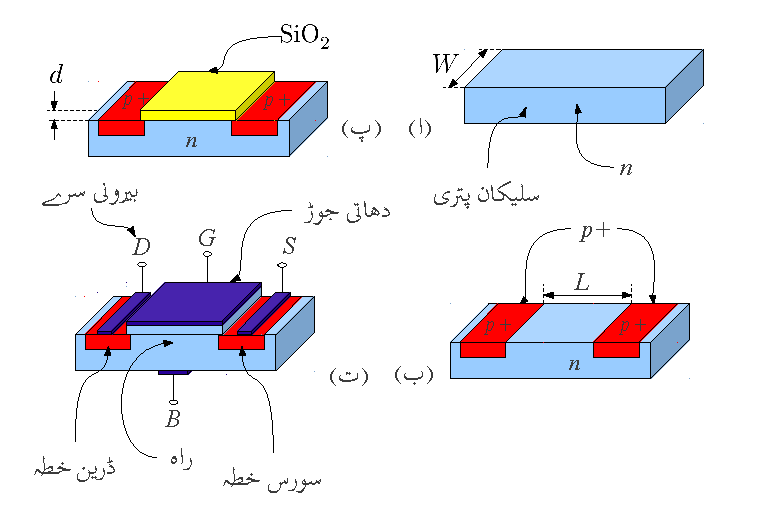
\includegraphics[scale=0.90]{pMOSFETstructure}
\caption{\عددی{p} ماسفیٹ کی ساخت}
\label{شکل_ماسفیٹ_مثبت_ساخت}
\end{figure}
%
\begin{figure}
\centering
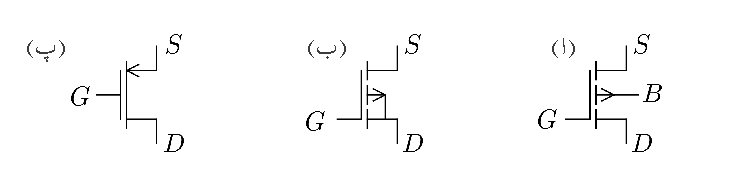
\includegraphics[scale=0.90]{pMosfetEnhancementSymbols}
\caption{\عددی{p} بڑھاتا ماسفیٹ کی علامتیں}
\label{شکل_ماسفیٹ_مثبت_بڑھاتا_علامتیں}
\end{figure}


\عددی{\textup{nMOSFET}}  کی جسامت کم ہونے کی بدولت سلیکان پتری پر انہیں زیادہ تعداد میں بنایا جا سکتا ہے۔یوں اگرچہ مخلوط ادوار میں  \عددی{\textup{nMOSFET}} کو \عددی{\textup{pMOSFET}} پر ترجیح دی جاتی ہے مگر پھر بھی ان کی اپنی اہمیت ہے جس کی بنا پر انہیں بھی مخلوط ادوار میں استعمال کیا جاتا ہے۔بالخصوص جڑوا ماسفیٹ  (CMOS) ادوار جو کہ اہم ترین ادوار تصور کئے جاتے ہیں ان دونوں اقسام کو استعمال کرتے ہی بنائے جاتے ہیں۔
\begin{figure}
\centering
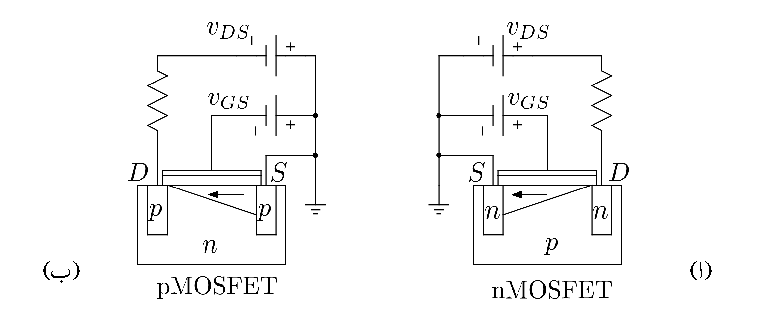
\includegraphics[scale=0.90]{mosfetEnhancementChannelNandP}
\caption{بڑھاتے \تحریر{nMOSFET} اور  \تحریر{pMOSFET} نقطہ دبوچ پر}
\label{شکل_ماسفیٹ_منفی_اور_مثبت_راہ}
\end{figure}

شکل \حوالہ{شکل_ماسفیٹ_منفی_اور_مثبت_راہ} میں موازنے کے لئے بڑھاتے \تحریر{nMOSFET} اور \تحریر{pMOSFET} کو نقطہ دبوچ پر مائل کرتے دکھائے گئے ہیں۔\تحریر{nMOSFET} میں سورس \تحریر{S} کو برقی زمین پر رکھا گیا ہے۔پیدا کردہ راہ میں برقی رو کو تیر کے نشان سے دکھایا گیا ہے۔یوں اگر راہ کا بایاں سرا صفر وولٹ پر  ہو تو اس کا دایاں سرا مثبت برقی دباو پر ہو گا۔یوں گیٹ اور بائیں سرے کے مابین برقی دباو زیادہ ہو گا جبکہ گیٹ اور دائیں سرے کے مابین برقی دباو نسبتاً کم ہو گا جس سے راہ ترچھی شکل کا پیدا ہو گا۔جہاں گیٹ اور سلیکان کے مابین برقی دباو زیادہ ہو وہاں راہ کی گہرائی زیادہ ہو گی۔\تحریر{pMOSFET} میں بھی سورس \تحریر{S} کو برقی زمین پر رکھا گیا ہے۔پیدا کردہ راہ میں برقی رو کو تیر کے نشان سے دکھایا گیا ہے۔یوں اگر راہ کا دایاں سرا صفر وولٹ پر  ہو تو اس کا بایاں سرا منفی برقی دباو پر ہو گا۔یوں گیٹ اور دائیں سرے کے مابین برقی دباو زیادہ ہو گا جبکہ گیٹ اور بائیں سرے کے مابین برقی دباو نسبتاً کم ہو گا۔جہاں گیٹ اور سلیکان کے مابین برقی دباو زیادہ ہو وہاں راہ کی گہرائی زیادہ ہو گی۔آپ دیکھ سکتے ہیں کہ دونوں اقسام کے ماسفیٹ میں پیدا کردہ راہ ڈرین پر دبوچہ جاتا ہے۔

\تحریر{pMOSFET} کے \عددی{v_{GS}}، \عددی{v_{DS}} اور \عددی{i_{DS}} منفی مقداریں ہیں لہٰذا \عددی{v_{SG}}، \عددی{v_{SD}} اور \عددی{i_{SD}} مثبت مقدار ہوں گے۔\تحریر{pMOSFET} کے مساوات مندرجہ ذیل ہیں۔

\جزوحصہ{غیر افزائندہ}
\begin{gather}
\begin{aligned} \label{مساوات_ماسفیٹ_جمع_غیر_افزائندہ_حدود_و_مساوات}
v_{SG}& >  -V_t \\
v_{DG}& \ge -V_t\\
i_{SD}&=k_p' \left[\frac{W}{L} \right ] \left[\left(v_{SG}+V_t \right )v_{SD}-\frac{v_{SD}^{2}}{2} \right ]
\end{aligned}
\end{gather}

\جزوحصہء{نقطہ  دبوچ}
\begin{gather}
\begin{aligned}
v_{SG}& > -V_t\\
v_{DG}&=-V_t\\
i_{SD}&=\frac{k_p'}{2} \left[\frac{W}{L} \right ] \left[v_{SG}+V_t \right]^{2} 
\end{aligned}
\end{gather}
\جزوحصہء{افزائندہ}
\begin{gather}
\begin{aligned}\label{مساوات_ماسفیٹ_منفی_ماسفیٹ_افزائنہ_صورت_مثبت_متغیرات}
v_{SG}& > -V_t\\
v_{DG}& \le -V_t \\
i_{SD}&=\frac{k_p'}{2} \left[\frac{W}{L} \right ] \left[v_{SG}+V_t \right]^{2}
\end{aligned}
\end{gather}
\جزوحصہء{منقطع}
\begin{gather}
\begin{aligned}
v_{SG}&\le  -V_t\\
i_{SD}&=0
\end{aligned}
\end{gather}
%==============
\حصہ{گھٹاتا  \عددی{n} ماسفیٹ}
\تحریر{nMOSFET} بناتے وقت، اس کے سورس اور ڈرین خطوں کے درمیان سلیکان پتری میں گیٹ کے بالکل نیچے \عددی{n} قسم کے خطے کے اضافہ سے \عددی{n}  قسم کا \اصطلاح {ماسفیٹ!گھٹاتا}\فرہنگ{گھٹاتا ماسفیٹ}\فرہنگ{depletion nMOSFET}\حاشیہب{depletion nMOSFET}  وجود میں آتا ہے۔شکل \حوالہ{شکل_ماسفیٹ_کی_علامتیں} الف میں \عددی{n} قسم کے \اصطلاح {گھٹاتے ماسفیٹ} کی علامت دکھائی گئی ہے۔\اصطلاح {گھٹاتے ماسفیٹ} کی علامت میں راہ کو موٹی لکیر سے ظاہر کیا جاتا ہے۔شکل  الف میں \عددی{n} گھٹاتا ماسفیٹ کی علامت دکھائی گئی ہے۔ساتھ ہی موازنے کی خاطر \عددی{n} بڑھاتے ماسفیٹ کی علامت بھی دکھائی گئی ہے۔ 

\begin{figure}
\centering
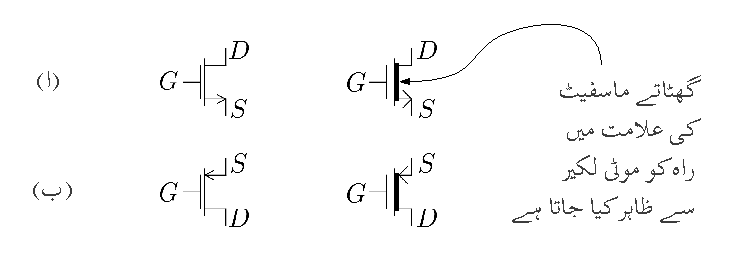
\includegraphics[scale=0.90]{mosfetEnhancementAndDepletionSymbols}
\caption{گھٹاتے اور بڑھاتے ماسفیٹ کی علامتیں}
\label{شکل_ماسفیٹ_کی_علامتیں}
\end{figure}

چونکہ \اصطلاح {گھٹاتا ماسفیٹ} میں پہلے سے ہی سورس اور ڈرین خطوں کے مابین راہ موجود ہوتا ہے لہٰذا گیٹ پر صفر وولٹ \عددی{(v_{GS}=0)} ہوتے ہوئے بھی اگر سورس اور ڈرین سروں  کے مابین برقی دباو \عددی{v_{DS}}  لاگو کی جائے تو ماسفیٹ میں برقی رو \عددی{i_{DS}} گزرے گا۔گیٹ پر برقی دباو بڑھانے سے راہ کی گہرائی بڑھتی ہے جس سے برقی رو میں اضافہ ہوتا ہے جبکہ گیٹ پر منفی برقی دباو لاگو کرنے سے راہ کی گہرائی گھٹتی ہے جس سے \عددی{i_{DS}}  میں کمی آتی ہے۔اسی سے اس کا نام \عددی{n} \اصطلاح {قسم کا  گھٹاتا ماسفیٹ}  نکلا ہے۔اگر گیٹ پر لاگو برقی دباو کو بتدریج منفی جانب لے جایا جائے تو آخر کار راہ کی گہرائی صفر ہو جائے گی اور ماسفیٹ میں برقی رو کا گزرنا ممکن نہیں رہے گا۔یہ برقی دباو اس ماسفیٹ کا \عددی{V_t} ہوتا ہے۔یوں \عددی{n}  قسم کے گھٹاتا ماسفیٹ کا \عددی{V_t} منفی قیمت رکھتا ہے۔

گھٹاتا اور بڑھاتا منفی ماسفیٹ کے مساوات میں کوئی فرق نہیں لہٰذا اب تک  کے تمام بڑھاتا ماسفیٹ کے مساوات جوں کے توں گھٹاتا ماسفیٹ کے لئے بھی استعمال کئے جائیں گے۔ 

\جزوحصہ{منقطع صورت}
اگر گھٹاتا ماسفیٹ کے \عددی{v_{GS}} پر \عددی{V_t} سے کم (یعنی مزید منفی) برقی دباو لاگو کیا جائے تو راہ کا وجود نہیں رہے گا یعنی پیدا کردہ راہ نہیں رہے گا اور ماسفیٹ \اصطلاح {منقطع صورت}\حاشیہب{cut off state}  اختیار کر لے گا۔ اس شرط کو یوں بیان کیا جاتا ہے۔
\begin{align}
v_{GS} \le V_t
\end{align}

یوں اگر کسی گھٹاتا ماسفیٹ کا \عددی{V_t=\SI{-3.5}{\volt}} ہو اور اس کے گیٹ پر \عددی{v_{GS}=\SI{-4}{\volt}} لاگو کیا جائے تو یہ \اصطلاح {منقطع} ہو جائے گا اور اگر اس کے گیٹ پر \عددی{v_{GS}=\SI{-2.2}{\volt}} یا \عددی{v_{GS}=\SI{+1.2}{\volt}} اور یا \عددی{v_{GS}=\SI{+5.3}{\volt}} لاگو کیا جائے تو ماسفیٹ چالو رہے گا۔
\جزوحصہ{غیر افزائندہ}
\عددی{v_{GS}} پر \عددی{V_t}  سے زیادہ برقی دباو لاگو کرنے سے ماسفیٹ چالو حالت اختیار کر لیتا ہے۔جب تک چالو ماسفیٹ کے گیٹ پر ڈرین خطے سے \عددی{\abs{V_t}} وولٹ کم نہ ہو جائیں گھٹاتا ماسفیٹ غیر افزائندہ ہو گا۔اس شرط کو یوں بیان کیا جاتا ہے۔
\begin{gather}
\begin{aligned}
v_{GS}-v_{DS} \ge V_t \\
v_{GD} \ge V_t
\end{aligned}
\end{gather}

یوں اسی مثال کو آگے بڑھاتے ہوئے اگر \عددی{V_t=\SI{-3.5}{\volt}} ہو اور  \عددی{v_{GS}=\SI{+5.3}{\volt}} ہو تب جب تک  \عددی{v_{DS}<\SI{8.8}{\volt}} رہے ماسفیٹ غیر افزائندہ رہے گا۔
\جزوحصہ{دبوچ}
جب گیٹ پر ڈرین سے \عددی{\abs{V_t}} وولٹ کم ہو جائیں تو پیدا کردہ راہ دبوچا جاتا ہے۔اس شرط کو یوں بیان کرتے ہیں۔
\begin{gather}
\begin{aligned}
v_{GS}-v_{DS}=V_t\\
v_{GD} =V_t
\end{aligned}
\end{gather}

یوں \عددی{V_t=\SI{-3.5}{\volt}}  اور \عددی{v_{GS}=\SI{+5.3}{\volt}} کی صورت میں جب  \عددی{v_{DS}=\SI{8.8}{\volt}} ہو تب پیدا کردہ راہ دبوچا جائے گا۔
\جزوحصہ{افزائندہ} 
	جب چالو ماسفیٹ کے ڈرین پر گیٹ سے \عددی{\abs{V_t}}	وولٹ زیادہ ہوں تب یہ افزائندہ حال میں ہو گا۔اس شرط کو یوں بیان کرتے ہیں۔
\begin{gather}
\begin{aligned}
v_{GS}-v_{DS} \le V_t \\
v_{GD} \le V_t
\end{aligned}
\end{gather}
یوں  \عددی{V_t=\SI{-3.5}{\volt}} اور \عددی{v_{GS}=\SI{+5.3}{\volt}}  کی صورت میں جب \عددی{v_{DS}>\SI{8.8}{\volt}} ہو تب ماسفیٹ افزائندہ خطے میں ہو گا۔

یہاں تسلی کر لیں کہ گھٹاتا ماسفیٹ کے مختلف خِطوں کی مساواتیں بالکل وہی ہیں جو عام ماسفیٹ کی ہیں۔فرق صرف اتنا ہے کہ گھٹاتا ماسفیٹ کے \عددی{V_t} کی قیمت منفی ہوتی ہے۔

\حصہ{گھٹاتا \عددی{p} ماسفیٹ}
\عددی{p} قسم کا گھٹاتا ماسفیٹ اسی طرح \عددی{p} ماسفیٹ بناتے وقت سلیکان پتری میں گیٹ کے بالکل نیچے \عددی{p} قسم کی راہ، سورس سے ڈرین خطے تک بنانے سے پیدا ہوتا ہے۔ \عددی{p} قسم کے گھٹاتا ماسفیٹ اور عام \عددی{p} قسم کے ماسفیٹ کے مساوات ایک ہی طرح کے ہیں۔فرق صرف اتنا ہے کہ \عددی{p}  قسم کے گھٹاتا ماسفیٹ کی \عددی{V_t} کی قیمت مثبت ہوتی ہے۔مزید یہ کہ کسی بھی \عددی{p} قسم کے ماسفیٹ کی طرح \عددی{p}  قسم کے گھٹاتا ماسفیٹ میں برقی رو ڈرین سرے سے باہر کی جانب ہوتا ہے۔شکل \حوالہ{شکل_ماسفیٹ_کی_علامتیں} ب میں \عددی{p} قسم کے \اصطلاح {گھٹاتے ماسفیٹ} کی علامت دکھائی گئی ہے۔

%===========
\حصہ{جڑوا ماسفیٹ \تحریر{CMOS} }
\اصطلاح {جڑوا ماسفیٹ} \تحریر{nMOSFET}  اور \تحریر{pMOSFET}  دونوں استعمال کرتے بنتے ہیں جنہیں \عددی{p}  سلیکان پر بنایا جاتا ہے۔\تحریر{nMOSFET} تو بنتا ہی \عددی{p} سلیکان پر ہے البتہ \تحریر{pMOSFET} بناتے وقت پہلے \عددی{p} سلیکان میں گہرا \عددی{n} خطہ بنایا جاتا ہے اور پھر اس خطے میں \تحریر{pMOSFET} بنایا جاتا ہے۔شکل \حوالہ{شکل_ماسفیٹ_سیماس_کی_ساخت} میں \اصطلاح {جڑوا ماسفیٹ} کی ساخت دکھائی گئی ہے۔\اصطلاح {جڑوا ماسفیٹ} کو عام فہم میں \اصطلاح {سیماس}\فرہنگ{سیماس}\حاشیہب{CMOS}\فرہنگ{CMOS} کہتے ہیں۔شکل میں ماسفیٹ کے دونوں جانب \عددی{\ce{SiO2}} کے گہرے حصے دکھائے گئے ہیں جو ساتھ ساتھ دو ماسفیٹ کو مکمل طور پر علیحدہ رکھنے کی خاطر استعمال کئے جاتے ہیں۔یاد رہے کہ \عددی{\ce{SiO2}} نہایت عمدہ غیر موصل ہے۔سیماس کو \عددی{p} سلیکان پر بھی بنایا جا سکتا ہے۔پس اس میں \تحریر{pMOSFET} کو گہرے \عددی{n} خطے میں بنانا ہو گا جبکہ \تحریر{nMOSFET} تو بنتا ہی \عددی{p} سلیکان پر ہے۔ 
\begin{figure}
\centering
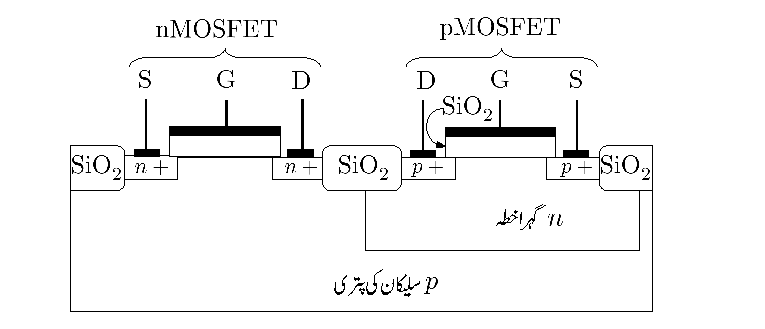
\includegraphics[scale=0.90]{cmosStructure}
\caption{سیماس یا جڑوا ماسفیٹ کی ساخت}
\label{شکل_ماسفیٹ_سیماس_کی_ساخت}
\end{figure}

%====================
\حصہ{ماسفیٹ کے یک سمتی ادوار کا حل}
اس حصے میں ماسفیٹ کے یک سمتی ادوار حل کئے جائیں گے۔جیسے اس کتاب کے شروع میں بتلایا گیا ہے، یک سمتی متغیرات انگریزی کے بڑے حروف سے ظاہر کئے جاتے ہیں۔یوں گیٹ پر برقی دباو کو \عددی{v_{GS}} کی جگہ \عددی{V_{GS}} لکھا جائے گا۔اسی طرح \عددی{v_{DS}} کو \عددی{V_{DS}} اور \عددی{i_{DS}} کو \عددی{I_{DS}} لکھا جائے گا۔

اس حصے میں دئے گئے مثالوں کو پہلے خود حل کرنے کی کوشش کریں اور بعد میں کتاب میں دئے حل دیکھیں۔

%=========
\ابتدا{مثال}
ایک منفی  گھٹاتا ماسفیٹ جس کا \عددیء{v_{DS}=\SI{1}{\volt}}، \عددی{V_{t}=\SI{-3.2}{\volt}} اور
 \عددی{k_n=\SI{0.1}{\milli \ampere \per \volt \squared }} ہیں کا برقی رو مندرجہ ذیل پر حاصل کریں۔
\begin{enumerate}
\item
\عددی{v_{GS}=\SI{-4}{\volt}}
\item
\عددی{v_{GS}=\SI{-3.2}{\volt}}
\item
\عددی{v_{GS}=\SI{-2.8}{\volt}}
\item
\عددی{v_{GS}=\SI{-2.2}{\volt}}
\item
\عددی{v_{GS}=\SI{+1.5}{\volt}}

\end{enumerate}



حل:
\begin{enumerate}
\item
\عددی{v_{GS}=\SI{-4}{\volt}} اور  \عددی{V_{t}=\SI{-3.2}{\volt}} ہیں۔چونکہ \عددی{(-4< -3.2)}  ہے لہٰذا \عددی{v_{GS}<V_t} ہے اور یوں گھٹاتا ماسفیٹ منقطع ہے اور اس میں برقی رو کا گزر ممکن نہیں ہے یعنی \عددی{i_{DS}=0} ہے۔
\item
\عددی{v_{GS}=\SI{-3.2}{\volt}} اور  \عددی{V_{t}=\SI{-3.2}{\volt}} ہونے کی وجہ سے \عددی{v_{GS}=V_t} ہے۔اس صورت پیدا کردہ راہ وجود میں آئے گا مگر اس کی گہرائی تقریباً صفر ہو گی اور اس میں برقی رو کا گزر ممکن نہیں ہے یعنی  \عددی{i_{DS}=0} ہے۔

\item

\عددی{v_{GS}=\SI{-2.8}{\volt}} اور  \عددی{V_{t}=\SI{-3.2}{\volt}}	 پر چونکہ  \عددی{(-2.8 > -3.2)} ہے لہٰذا \عددی{v_{GS}> V_t} ہے اور یوں گھٹاتا ماسفیٹ چالو ہے۔ \عددی{V_{DS}=\SI{+1}{\volt}} پر گیٹ اور ڈرین کے مابین برقی دباو
\begin{align*}
v_{GS}-v_{DS}=(-2.8)-(1)=\SI{-3.8}{\volt}
\end{align*}
ہے جو کہ  \عددی{V_t} سے کم ہے یعنی
\begin{align*}
v_{GS}-v_{DS}<V_t
\end{align*}
لہٰذا گھٹاتا ماسفیٹ افزائندہ ہے اور یوں
\begin{align*}
i_{DS}&=\frac{k_n}{2} \left[v_{GS}-V_t \right]^2 \\
&=\frac{0.1 \times 10^{-3}}{2} \times \left[(-2.8)-(-3.2) \right]\\
&=\SI{8}{\micro \ampere}
\end{align*}
\item
\عددی{v_{GS}=\SI{-2.2}{\volt}} اور  \عددی{V_{t}=\SI{-3.2}{\volt}}	 پر چونکہ  \عددی{(-2.2>-3.2)}  ہے لہٰذا \عددی{v_{GS}>V_t} ہے اور یوں گھٹاتا ماسفیٹ چالو ہے۔ \عددی{V_{DS}=+\SI{+1}{\volt}} پر گیٹ اور ڈرین کے مابین برقی دباو
\begin{align*}
v_{GS}-v_{DS}=(-2.2)-(1)=\SI{-3.2}{\volt}
\end{align*}
ہے جو کہ \عددی{V_t} کے برابر ہے  یعنی
\begin{align*}
v_{GS}-v_{DS}=V_t
\end{align*}
لہٰذا گھٹاتا ماسفیٹ نقطہ دبوچ پر ہے۔یوں
\begin{align*}
i_{DS}&=\frac{k_n}{2} \left[v_{GS}-V_t \right ]^2  \\
&=\frac{0.1 \times 10^{-3}}{2} \left[(-2.2)-(-3.2) \right ]^2 \\
&=\SI{50}{\micro \ampere}
\end{align*}
\item
\عددی{v_{GS}=\SI{+1.5}{\volt}} اور  \عددی{V_{t}=\SI{-3.2}{\volt}}	 پر چونکہ  \عددی{(+1.5>-3.2)} ہے لہٰذا  \عددی{v_{GS}>V_t} ہے اور یوں گھٹاتا ماسفیٹ چالو ہے۔ \عددی{V_{DS}=\SI{+1}{\volt}} پر گیٹ اور ڈرین کے مابین برقی دباو
\begin{align*}
v_{GS}-v_{DS}=+1.5-1=\SI{+0.5}{\volt}
\end{align*}
ہے جو کہ \عددی{V_t} سے زیادہ ہے یعنی
\begin{align*}
v_{GS}-v_{DS} > V_t
\end{align*}
لہٰذا گھٹاتا ماسفیٹ غیر افزائندہ ہے۔یوں
\begin{align*}
i_{DS}&=k_n \left[\left(v_{GS}-V_t \right )v_{DS}-\frac{v_{DS}^{2}}{2} \right ]\\
&=0.1 \times 10^{-3} \times \left[\left(1.5-(-3.2) \right ) \times  1 - \frac{1^2}{2} \right ]\\
&=\SI{0.42}{\milli \ampere}
\end{align*}

\end{enumerate}

\انتہا{مثال}
%=================


\ابتدا{مثال}
شکل \حوالہ{شکل_ماسفیٹ_کے_یک_سمتی_ادوار_الف} الف میں منفی بڑھاتا ماسفیٹ کے گیٹ کو سورس کے ساتھ جوڑ کر دور بنایا گیا ہے۔اس ماسفیٹ کا  \عددی{V_t=\SI{3}{\volt}}  اور \عددی{k_n=\SI{0.2}{\milli \ampere \volt^{-2}}} ہیں جبکہ دور میں \عددی{V_{\textup{DD}}=\SI{10}{\volt}} ہے۔ دور میں برقی رو حاصل کریں۔
\begin{figure}
\centering
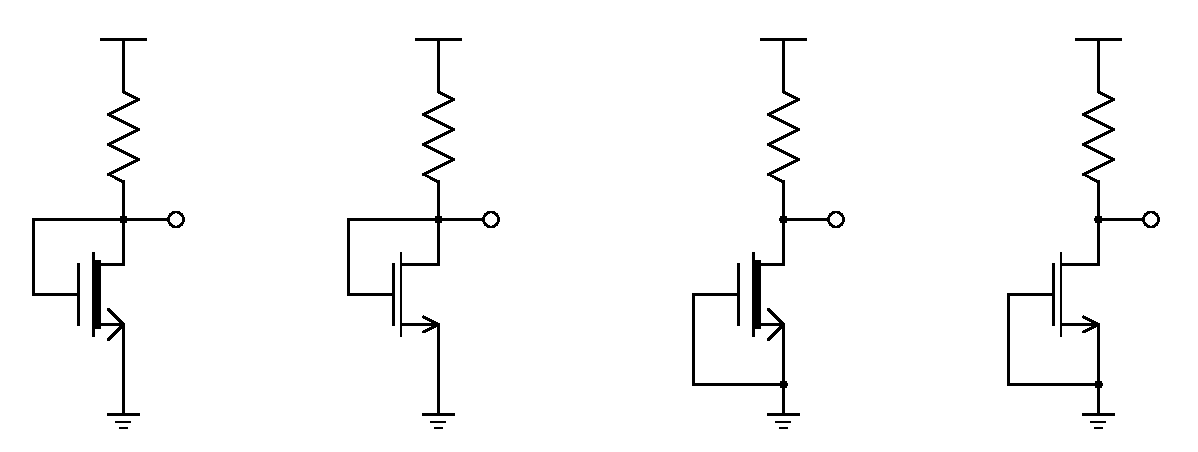
\includegraphics[scale=0.90]{mosfetDCcircuitsA}
\caption{ماسفیٹ کے یک سمتی ادوار}
\label{شکل_ماسفیٹ_کے_یک_سمتی_ادوار_الف}
\end{figure}
حل: \عددی{n} قسم کے بڑھاتا ماسفیٹ کے \عددی{V_t}  کی قیمت ہر صورت مثبت ہوتی ہے۔ \عددی{n} قسم کے ماسفیٹ کا گیٹ اور سورس آپس میں جوڑنے سے \عددی{V_{\textup{GS}}=0} ہو جاتا ہے اور یوں  \عددی{V_{\textup{GS}} < V_t}  ہوتا ہے جس سے ماسفیٹ منقطع ہو جاتا ہے اور  \عددی{I_{DS}=0}  ہوتا ہے۔

\انتہا{مثال}
%==========
\ابتدا{مثال}
شکل \حوالہ{شکل_ماسفیٹ_کے_یک_سمتی_ادوار_الف} ب میں منفی گھٹاتا ماسفیٹ کے گیٹ کو سورس کے ساتھ جوڑ کر دور بنایا گیا ہے۔اس ماسفیٹ کا \عددی{V_t=\SI{-3}{\volt}} اور \عددی{k_n=\SI{0.2}{\milli \ampere \volt^{-2}}} ہیں  جبکہ دور میں \عددی{V_{\textup{DD}}=\SI{10}{\volt}}  ہے۔دور میں برقی رو حاصل کریں۔

حل: \عددی{n} قسم کے گھٹاتا ماسفیٹ کے \عددی{V_t}  کی قیمت ہر صورت منفی ہوتی ہے۔ \عددی{n} قسم کے ماسفیٹ کا گیٹ اور سورس آپس میں جوڑنے سے  \عددی{V_{\textup{GS}}=0}  ہو جاتا ہے اور یوں \عددی{V_{\textup{GS}}>V_t}  یعنی ماسفیٹ چالو ہوتا ہے۔اب یہ دیکھنا ہو گا کہ آیا یہ ماسفیٹ افزائندہ خطے میں ہے یا کہ غیر افزائندہ خطے میں۔

ماسفیٹ کے سوالات میں عموماً قبل از وقت یہ جاننا ممکن نہیں ہوتا کہ ماسفیٹ افزائندہ یا غیر افزائندہ خطے میں ہے۔یوں آپ جان نہیں سکتے کہ ماسفیٹ کی برقی رو حاصل کرتے وقت افزائندہ ماسفیٹ کی مساوات یا غیر افزائندہ ماسفیٹ کی مساوات استعمال ہو گی۔

اس طرح کے سوالات حل کرتے وقت آپ تصور کریں گے کہ ماسفیٹ افزائندہ (یا غیر افزائندہ) خطے میں ہے\حاشیہد{میری عادت ہے کہ میں ماسفیٹ کو افزائندہ تصور کر کے دور حل کرنے کی کوشش پہلے کرتا ہوں۔} اور پھر دور حل کرنے کی کوشش کریں گے۔حل کرنے کے بعد دوبارہ تسلی کریں گے کہ ماسفیٹ افزائندہ (یا غیر افزائندہ ) خطے میں ہی ہے۔اگر حتمی جواب اور تصور کردہ صورتیں یکساں نکل آئیں تو حل تسلیم کر لیا جاتا ہے ورنہ ماسفیٹ کو غیر افزائندہ (افزائندہ) تصور کر کے دور کو دوبارہ حل کیا جاتا ہے۔آئیں اس ترکیب کو استعمال کریں۔

ہم تصور کرتے ہیں کہ گھٹاتا ماسفیٹ افزائندہ خطے میں ہے۔یوں مساوات \حوالہ{مساوات_میدانی_افزائندہ_رو}  کے تحت
\begin{align*}
I_{DS}=\frac{k_n}{2} \left(V_{GS}-V_t \right )^{2}=\frac{0.2 \times 10^{-3}}{2} \left(0-(-3) \right )^2 =\SI{0.9}{\milli \ampere}
\end{align*}
اور شکل  ب میں خارجی جانب کرچاف کا قانون برائے برقی دباو استعمال کرتے ہوئے
\begin{align*}
V_{DD}&=I_{DS} R_D+V_{DS}\\
10&=0.9 \times 10^{-3} \times 4.7 \times 10^{3}+V_{DS}\\
V_{DS}&=\SI{5.77}{\volt}
\end{align*}
حاصل ہوتا ہے۔

اس جواب کو استعمال کرتے ہوئے ہم نے یہ دیکھنا ہو گا کہ آیا ماسفیٹ واقعی افزائندہ ہے یا نہیں۔مساوات \حوالہ{مساوات_میدانی_کارکردگی_کے_خطے}  کا آخری جزو افزائندہ ماسفیٹ کی شرط بیان کرتا ہے۔موجودہ مثال میں
\begin{align*}
V_{GS}-V_{DS}=0-5.77=\SI{-5.77}{\volt}
\end{align*}
ہے جبکہ  \عددی{V_t=\SI{-3}{\volt}} ہے۔یوں  \عددی{V_{GS}-V_{DS}< V_t} کی شرط پوری ہوتی ہے اور ماسفیٹ یقیناً افزائندہ ہی ہے لہٰذا \عددی{I_{DS}=\SI{0.9}{\milli \ampere}} ہی صحیح جواب ہے۔

آئیں اسی مثال میں ماسفیٹ کو غیر افزائندہ تصور کر کے مثال کو دوبارہ حل کرتے ہیں۔غیر افزائندہ ماسفیٹ کی مساوات حل کرنے کی خاطر  \عددی{V_{DS}} کا معلوم ہونا ضروری ہے۔دور کے خارجی جانب کرچاف کے قانون برائے برقی دباو سے ملتا ہے
\begin{align*}
V_{DD}&=I_{DS} R_D+V_{DS}\\
10&=I_{DS} \times 4.7 \times 10^{3}+V_{DS}\\
V_{DS}&=10-4700 I_{DS}
\end{align*}
غیر افزائندہ ماسفیٹ کے مساوات میں \عددی{V_{DS}} کی جگہ اسے استعمال کرتے حل کرتے ہیں۔
\begin{align*}
I_{DS}&=k_n \left[\left(V_{GS}-V_t \right )V_{DS} -\frac{V_{DS}^{2}}{2}\right ]\\
\frac{I_{DS}}{k_n}&=\left[\left(V_{GS}-V_t \right )V_{DS} -\frac{V_{DS}^{2}}{2}\right ]\\
\frac{I_{DS}}{0.2 \times 10^{-3}}&=\left[\left(0-(-3) \right ) \left(10-4700 I_{DS} \right )- \frac{\left( 10-4700 I_{DS} \right )^{2}}{2}\right]
\end{align*}
سے
\begin{align*}
I_{DS}&=1.26\mp j 0.46 \,{\milli \ampere}
\end{align*}
حاصل ہوتا ہے۔یہ مخلوط جوابات ہیں۔ غیر حقیقی برقی رو معنی نہیں رکھتی لہٰذا ماسفیٹ کے غیر افزائندہ ہونے کو رد کیا جاتا ہے۔
\انتہا{مثال}
%========
\ابتدا{مثال} \شناخت{مثال_میدانی_گیٹ_اور_محاصل_جڑے}
شکل \حوالہ{شکل_ماسفیٹ_کے_یک_سمتی_ادوار_الف} پ میں منفی بڑھاتا ماسفیٹ کے ڈرین اور گیٹ جوڑ کر یک سمتی دور بنایا گیا ہے۔اس ماسفیٹ کا \عددی{V_t=\SI{3}{\volt}} اور \عددی{k_n=\SI{0.2}{\milli \ampere \volt^{-2}}} ہیں  جبکہ دور میں \عددی{V_{DD}=\SI{10}{\volt}}  ہے۔دور میں برقی رو حاصل کریں۔

حل:	گیٹ اور ڈرین جوڑنے سے گیٹ اور ڈرین برابر برقی دباو پر ہوں گے یعنی 
\begin{align*}
V_{GS}=V_{DS}
\end{align*}
ہو گا۔یوں  \عددی{V_{GS}-V_{DS}=0}  ہو گا اور یوں \عددی{V_{GS}-V_{DS}<V_t} ہو گا۔اس طرح ماسفیٹ افزائندہ ہو گا اور ہم برقی رو
\begin{align*}
I_{DS}=\frac{k_n}{2}\left(V_{GS}-V_t \right )^{2}
\end{align*}
سے حاصل کر سکتے ہیں۔البتہ ایسا کرنے کی خاطر ہمیں \عددی{V_{GS}} کی قیمت درکار ہو گی۔شکل  پ کے خارجی جانب کرچاف کے قانون برائے برقی دباو کے استعمال سے 
\begin{align*}
V_{DD}=I_{DS} R_D+V_{DS}
\end{align*}
حاصل ہوتا ہے۔چونکہ اس مثال میں \عددی{V_{GS}=V_{DS}}  ہے لہٰذا اس مساوات کو یوں لکھ سکتے ہیں
\begin{align*}
V_{DD}&=I_{DS}R_D+V_{GS}\\
10&=I_{DS} \times 4.7 \times 10^{3}+V_{GS}\\
V_{GS}&=10-4700 I_{DS}
\end{align*}
اس مساوات کو افزائندہ ماسفیٹ کے مساوات کے ساتھ حل کرنے سے برقی رو حاصل کی جا سکتی ہے۔اس مساوات سے حاصل \عددی{V_{GS}} کو افزائندہ ماسفیٹ کے مساوات میں استعمال کرتے ہیں
\begin{align*}
I_{DS}&=\frac{k_n}{2} \left(V_{GS}-V_t \right )^2\\
\frac{2 I_{DS}}{k_n}&= \left(V_{GS}-V_t \right )^2\\
& 22090000I_{DS}^{2}-75800 I_{DS}+49=0\\
& I_{DS}=\SI{2.567}{\milli \ampere}, \SI{0.8639}{\milli \ampere}
\end{align*}
ان دو جوابات سے \عددی{V_{DS}} کے دو قیمتیں حاصل ہوتی ہیں۔
\begin{align*}
V_{DS}&=V_{GS}=10-2.567 \times 10^{-3} \times 4700=\SI{-2.06}{\volt}\\
V_{DS}&=V_{GS}=10-0.8639 \times 10^{-3} \times 4700=\SI{5.94}{\volt}
\end{align*}
ان میں پہلے جواب کے مطابق \عددی{V_{GS} =\SI{-2.06}{\volt}} ہے جس سے \عددی{V_{GS}<V_t} حاصل ہوتا ہے۔اگر ایسا ہوتا تو ماسفیٹ منقطع ہوتا اور اس میں برقی رو کا گزر ممکن ہی نہیں ہوتا لہٰذا یہ جواب غلط ہے۔دوسرے جواب کے مطابق   \عددی{V_{GS}=\SI{5.94}{\volt}} حاصل ہوا ہے اور یوں \عددی{V_{GS}>V_t} ہے۔اس طرح ماسفیٹ چالو حال میں ہے اور جواب تسلیم کرنا ہو گا۔


\انتہا{مثال}

%===========
\ابتدا{مثال} \شناخت{مثال_میدانی_برقی_رو_الف}
شکل \حوالہ{شکل_ماسفیٹ_کے_یک_سمتی_ادوار_الف} ت میں منفی گھٹاتا ماسفیٹ کا گیٹ اور ڈرین جوڑ کر دور بنایا گیا ہے۔اس ماسفیٹ کا \عددی{V_t=\SI{-3}{\volt}} اور \عددی{k_n=\SI{0.2}{\milli \ampere \volt^{-2}}} ہیں  جبکہ دور میں \عددی{{V_{DD}=\SI{10}{\volt}}} ہے۔دور میں برقی رو حاصل کریں۔

حل:	اس مثال میں خارجی جانب کرچاف کے قانون برائے برقی دباو کے تحت
\begin{align*}
V_{DD}&=I_{DS}R_D+V_{DS}\\
10&=I_{DS}\times 4700+V_{DS}
\end{align*}
حاصل ہوتا ہے۔چونکہ گیٹ اور ڈرین آپس میں جڑے ہیں لہٰذا ان پر برابر برقی دباو پایا جائے گا یعنی  \عددی{V_{GS}=V_{DS}} ہو گا اور اس مساوات کو یوں بھی لکھ سکتے ہیں۔
\begin{align*}
V_{DD}&=I_{DS}R_D+V_{GS}\\
10&=I_{DS} \times 4700+V_{GS}\\
V_{GS}&=10-4700 I_{DS}
\end{align*}
اگر ماسفیٹ منقطع ہو تب برقی رو کی مقدار صفر ہو گی اور اس صورت میں اس مساوات کے تحت \عددی{V_{GS}=\SI{10}{\volt}}  حاصل ہوتا ہے۔گھٹاتا ماسفیٹ کا   \عددی{V_t} منفی ہوتا ہے اور یوں یہاں \عددی{V_{GS}>V_t} ہے جو کہ چالو ماسفیٹ کی نشانی ہے۔یوں اس ماسفیٹ کو منقطع تصور کرنا غلط ہے۔آئیں اب دیکھتے ہیں کہ آیا ماسفیٹ افزائندہ یا غیر افزائندہ خطے میں ہے۔

گیٹ اور ڈرین آپس میں جڑے ہونے کی وجہ سے \عددی{V_{GS}-V_{DS}=0} ہو گا۔چونکہ گھٹاتا ماسفیٹ کا \عددی{V_t} منفی مقدار ہوتا ہے لہٰذا \عددی{V_{GS}-V_{DS}>V_t}  ہو گا اور یوں اگر یہ ماسفیٹ چالو  ہو تو یہ ہر صورت  غیر افزائندہ خطے میں ہو گا اور اس کی مساوات غیر افزائندہ ماسفیٹ کی مساوات سے حاصل کی جا سکتی ہے۔
\begin{align*}
I_{DS}&=k_n \left[\left(V_{GS}-V_t \right )V_{DS}-\frac{V_{DS}^2}{2}\right]\\
\frac{2 I_{DS}}{k_n}&=\left(10-4700 I_{DS}+3 \right )(10-4700I_{DS})-\frac{(10-4700I_{DS})^2}{2}\\
& I_{DS}=\SI{1.45}{\milli \ampere} , \SI{4.98}{\milli \ampere}
\end{align*}
ہم جانتے ہیں کہ اگر یہاں ماسفیٹ چالو ہو تب یہ غیر افزائندہ ہو گا لہٰذا دیکھنا یہ ہے کہ آیا ماسفیٹ چالو ہے یا نہیں۔

اگر \عددی{I_{DS}=\SI{4.98}{\milli\ampere}} ہو تب 	
\begin{align*}
V_{GS}&=10-4700 I_{DS}\\
&=10-4700 \times 4.98 \times 10^{-3}\\
&=\SI{-13}{\volt}
\end{align*}
اور یوں \عددی{V_{GS}<V_t} ہو گا جو کہ منقطع ماسفیٹ کی نشانی ہے۔منقطع ماسفیٹ برقی رو گزار ہی نہیں سکتا لہٰذا اس جواب کو رد کیا جاتا ہے۔

اگر \عددی{I_{DS}=\SI{1.45}{\milli \ampere}} ہو تب 	
\begin{align*}
V_{GS}&=10-4700 I_{DS}\\
&=10-4700 \times 1.45 \times 10^{-3}\\
&=\SI{3.2}{\volt}
\end{align*}
اور یوں \عددی{V_{GS}>V_t} ہو گا جو کہ چالو ماسفیٹ کی نشانی ہے۔یوں \عددی{{I_{DS}=\SI{1.45}{\milli \ampere}}} ہی درست جواب ہے۔

\انتہا{مثال}
%========

\ابتدا{مثال}
شکل \حوالہ{شکل_ماسفیٹ_کے_یک_سمتی_ادوار_الف} پ میں
\begin{align*}
k_n&=\SI{0.15}{\milli \ampere \volt^{-2}}\\
V_t&=\SI{3.5}{\volt}\\
V_{DD}&=\SI{10}{\volt}
\end{align*}
ہیں۔برقی رو \عددی{I_{DS}=\SI{0.6}{\milli \ampere}} حاصل کرنے کی خاطر  \عددی{R_{D}} کی قیمت دریافت کریں۔

حل:	جیسے مثال \حوالہ{مثال_میدانی_برقی_رو_الف}  میں ثابت کیا گیا، بڑھاتا \عددی{n} ماسفیٹ کا گیٹ اور ڈرین جوڑنے سے ماسفیٹ چالو حال میں رہتا ہے۔مزید یہ کہ یہ افزائندہ  ہوتا ہے جیسے مندرجہ ذیل مساوات سے دیکھا جا سکتا ہے۔
\begin{align*}
V_{GS}&=V_{DS}\\
V_{GS}-V_{DS}&=0\\
V_{GS}-V_{DS}&<V_t
\end{align*}
یوں افزائندہ ماسفیٹ کی مساوات استعمال کرتے ہوئے \عددی{V_{GS}}  کے لئے حل کرتے ہیں۔
\begin{align*}
I_{DS}&=\frac{k_n}{2}\left(V_{GS}-V_t \right )^2 \\
0.6 \times 10^{-3}&=\frac{0.15 \times 10^{-3}}{2} \left(V_{GS}-3 \right )^{2}\\
\frac{2 \times 0.6 \times 10^{-3}}{0.15 \times 10^{-3}}&=\left(V_{GS}-3 \right )^2 \\
8&=\left(V_{GS}-3 \right )^2 \\ 
V_{GS}&=\mp \sqrt{8} +3\\
V_{GS}&=\SI{0.172}{\volt}, \SI{5.828}{\volt}
\end{align*}
\عددی{V_{GS}=\SI{0.172}{\volt}} کے جواب کو رد کرتے ہیں چونکہ اس طرح  \عددی{V_{GS}< V_t} ہو گا اور ماسفیٹ منقطع ہو گا۔ \عددی{{V_{GS}=\SI{5.828}{\volt}}} کو تسلیم کرتے ہوئے دور کے خارجی جانب کرچاف کے قانون برائے برقی دباو میں \عددی{V_{DS}} کی قیمت کو حاصل شدہ  \عددی{V_{GS}} کی قیمت کے برابر لیتے ہوئے
\begin{align*}
V_{DD}&=I_{DS}R_{D} +V_{DS}\\
10&=0.6 \times 10^{-3} \times R_{D}+5.828\\
R_{D}&=\SI{6.95}{\kilo \ohm}
\end{align*}
حاصل ہوتا ہے۔

\انتہا{مثال}
%========

\ابتدا{مثال}
اگر شکل \حوالہ{شکل_ماسفیٹ_کے_یک_سمتی_ادوار_مثالیں} میں \عددیء{k_n=\SI{0.4}{\milli \ampere \volt^{-2}}} ، \عددیء{V_t=\SI{2.5}{\volt}}، \عددی{I_{DS}=\SI{0.8}{\milli \ampere}} اور \عددی{V_D=\SI{2}{\volt}} ہوں تو اس دور کے مزاحمت کی قیمت حاصل کریں۔
\begin{figure}
\centering
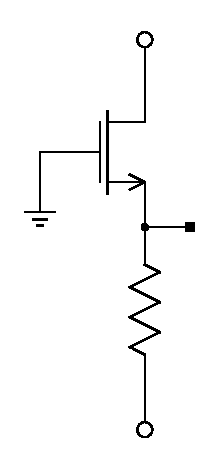
\includegraphics[scale=0.90]{mosfetExamples}
\caption{}
\label{شکل_ماسفیٹ_کے_یک_سمتی_ادوار_مثالیں}
\end{figure}

حل:	دور کے داخلی جانب کرچاف کے قانون برائے برقی دباو کے تحت
\begin{align*}
& V_{GS}+I_{DS}R_S-5=0\\
& V_{GS}=5-I_{DS}R_S
\end{align*}
اگر ماسفیٹ منقطع ہو تب برقی رو کی قیمت صفر ہو گی اور یوں
\begin{align*}
V_{GS}=5-I_{DS}R_S=5-0 \times R_S =\SI{5}{\volt}
\end{align*}
حاصل ہوتا ہے جس سے \عددی{V_{GS}>V_t}  ثابت ہوتا ہے جو کہ چالو ماسفیٹ کی نشانی ہے۔لہٰذا ماسفیٹ منقطع نہیں ہے۔

گیٹ برقی زمین پر ہے جبکہ ڈرین دو وولٹ پر ہے۔یوں
\begin{align*}
V_{GD}=V_{G}-V_{D}=0-2=\SI{-2}{\volt}
\end{align*}
حاصل ہوتا ہے اور یوں \عددی{V_{GD}<V_t} ثابت ہوتا ہے جو کہ افزائندہ ماسفیٹ کی نشانی ہے۔اس طرح افزائندہ ماسفیٹ کی مساوات استعمال ہو گی
\begin{align*}
I_{DS}&=\frac{k_n}{2} \left(V_{GS}-V_t \right )^{2}\\
I_{DS}&=\frac{k_n}{2} \left([5-I_{DS}R_S]-V_t \right )^{2}\\
0.8 \times 10^{-3}&=\frac{0.4 \times 10^{-3}}{2} \left(5-0.8 \times 10^{-3} \times R_S-2.5 \right )^{2}\\
\mp \sqrt{4}&=\left(2.5-0.8 \times 10^{-3} \times R_S \right )\\
R_S&=\SI{0.625}{\kilo \ohm},\hspace{2mm} \SI{5.625}{\kilo \ohm}
\end{align*}
اگر \عددی{R_S=\SI{0.625}{\kilo \ohm}} ہو تب
\begin{align*}
V_{GS}=5-I_{DS}R_S=5-0.8 \times 10^{-3} \times 0.625 \times 10^{3}=\SI{4.5}{\volt}
\end{align*}
ہو گا اور یوں \عددی{V_{GS}> V_t} ہو گا یعنی ماسفیٹ چالو ہو گا جو کہ قابل قبول جواب ہے۔اس کے برعکس اگر  \عددی{R_S=\SI{5.625}{\kilo \ohm}}
ہو تب
\begin{align*}
V_{GS}=5-I_{DS}R_S=5-0.8 \times 10^{-3} \times 5.625 \times 10^3 =\SI{0.5}{\volt}
\end{align*}
ہو گا اور یوں \عددی{V_{GS}<V_t} ہو گا یعنی ماسفیٹ منقطع ہو گا۔منقطع ماسفیٹ میں برقی رو کا گزر ممکن نہیں اور یوں یہ نا قابل قبول جواب ہے اور اسے رد کیا جاتا ہے۔

\انتہا{مثال}
%==========

\ابتدا{مثال}
شکل \حوالہ{شکل_ماسفیٹ_کے_یک_سمتی_ادوار_ب} الف میں دئے گئے دور کو اس طرح تخلیق کریں کہ  \عددی{I_{DS}=\SI{2}{\milli \ampere}} جبکہ \عددی{V_D=\SI{2}{\volt}} ہوں۔دور میں استعمال کئے گئے ماسفیٹ کی \عددی{V_t=\SI{3.3}{\volt}}  جبکہ اس کی  \عددی{k_n=\SI{0.6}{\milli \ampere \volt^{-2}}} ہے۔دور میں \عددی{V_{DD}=\SI{15}{\volt}} اور \عددی{V_{SS}=\SI{-10}{\volt}} رکھیں۔

حل: چونکہ گیٹ صفر جبکہ ڈرین دو وولٹ پر ہے لہٰذا \عددی{V_{GD}=\SI{-2}{\volt}} اور یوں  \عددی{V_{GD}<V_t} ہے جو کہ افزائندہ ماسفیٹ کی نشانی ہے۔یوں
\begin{align*}
I_{DS}&=\frac{k_n}{2} \left(V_{GS}-V_t \right )^{2}\\
2 \times 10^{-3}&=\frac{0.6 \times 10^{-3}}{2} \left(V_{GS}-3.3 \right )^{2}\\
V_{GS}&=3.3 \mp \sqrt{\frac{4}{0.6}}\\
V_{GS}&=\SI{0.718}{\volt}, \hspace{2mm} \SI{5.88}{\volt}
\end{align*}
اگر \عددی{V_{GS}=\SI{0.718}{\volt}}  لیا جائے تب  \عددی{V_{GS}<V_t} ہو گا اور ماسفیٹ منقطع ہو گا لہٰذا اس جواب کو رد کیا جاتا ہے۔یوں \عددی{V_{GS}=\SI{5.88}{\volt}} صحیح جواب ہے۔دور کے خارجی جانب کرچاف کے قانون برائے برقی دباو کے تحت
\begin{align*}
V_{GS}&=V_G  - V_S\\
5.88&=0-V_S\\
V_S&=\SI{-5.88}{\volt}
\end{align*}
یوں اُوہم کے قانون کے تحت
\begin{align*}
R_S=\frac{V_S-V_{SS}}{I_{DS}}=\frac{-5.88-(-10)}{2 \times 10^{-3}}=\SI{2.06}{\kilo \ohm}
\end{align*}
اور
\begin{align*}
R_D=\frac{V_{DD}-V_{D}}{I_{DS}}=\frac{15-2}{2 \times 10^{-3}}=\SI{6.5}{\kilo \ohm}
\end{align*}
حاصل ہوتے ہیں۔
\begin{figure}
\centering
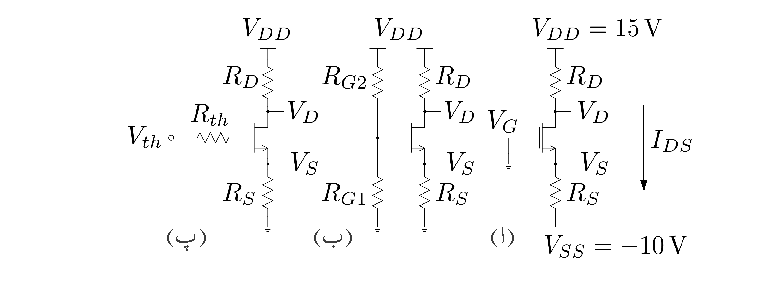
\includegraphics[scale=0.90]{mosfetDCcircuitsB}
\caption{ماسفیٹ کے مزید یک سمتی ادوار}
\label{شکل_ماسفیٹ_کے_یک_سمتی_ادوار_ب}
\end{figure}
\انتہا{مثال}
%=============
\ابتدا{مثال}
شکل \حوالہ{شکل_ماسفیٹ_کے_یک_سمتی_ادوار_ب} ب میں دو جوڑ ٹرانزسٹر مائل کرنے کے طرز پر گیٹ کے ساتھ دو مزاحمت منسلک کر کے ماسفیٹ کو مائل کیا گیا ہے۔اگر
\begin{align*}
V_{DD}&=\SI{12}{\volt}\\
R_D&=\SI{6.8}{\kilo \ohm}\\
R_S&=\SI{5.6}{\kilo \ohm}\\
R_{G1}&=R_{G2}=\SI{10}{\mega \ohm}\\
V_t&=\SI{2.5}{\volt}\\
k_n&=\SI{0.1}{\milli \ampere \volt \squared}
\end{align*}
ہوں تب اس دور میں تمام برقی دباو اور برقی رو حاصل کریں۔

حل:	شکل  پ میں اس کا مساوی تھوِنن دور دکھایا گیا ہے جہاں
\begin{align*}
V_{th}&=\frac{R_{G1} V_{DD}}{R_{G1}+R_{G2}}=\SI{6}{\volt}\\
R_{th}&=\frac{R_{G1} R_{G2}}{R_{G1}+R_{G2}}=\SI{5}{\mega \ohm}
\end{align*}
چونکہ ماسفیٹ کے گیٹ پر برقی رو کی قیمت صفر ہوتی ہے  \عددی{(I_G=0)}  لہٰذا ماسفیٹ کے گیٹ پر برقی دباو اسی تھونن برقی دباو کے برابر ہو گا یعنی
\begin{align*}
V_G=\SI{6}{\volt}
\end{align*}
شکل  ب میں گیٹ کو کھلے سرے تصور کرتے ہوئے \عددی{R_1} اور \عددی{R_2} کے جوڑ پر یہی \عددی{\SI{6}{\volt}} پائے جائیں گے۔یوں ماسفیٹ کے ادوار حل کرتے ہوئے تھونن مساوی دور بنانا لازم نہیں اور شکل  ب پر ہی گیٹ پر \عددی{\SI{6}{\volt}} لکھ کر آگے بڑھا جا سکتا ہے۔

خارجی جانب مزاحمت پر اُوہم کا قانون لاگو کرنے سے ماسفیٹ کے سورس اور ڈرین سروں پر برقی دباو کے مندرجہ ذیل کلیات حاصل ہوتے ہیں۔
\begin{align*}
V_{DD}-V_{D}=I_{DS}R_D\\
V_D=V_{DD}-I_{DS}R_D\\
V_D=12  - 6800 I_{DS}\\
\\
V_S=I_{DS}R_S=5600I_{DS}
\end{align*}
یوں
\begin{align*}
V_{GS}&=V_G -V_S = (6)-(5600 I_{DS})\\
V_{GD}&=V_G -V_D = (6)-\left(12-6800I_{DS} \right )=-6+6800I_{DS}
\end{align*}
ہو گا۔ان معلومات کے ساتھ رہتے ہوئے ہم یہ نہیں کہہ سکتے کہ ماسفیٹ افزائندہ یا غیر افزائندہ خطے میں ہے۔اس طرح کے مسائل میں ہم ماسفیٹ کو افزائندہ (غیر افزائندہ) تصور کر کے دور کو حل کرتے ہیں۔حتمی جواب حاصل ہونے کے بعد دوبارہ دیکھتے ہیں کہ آیا ماسفیٹ افزائندہ (غیر افزائندہ ) ہی ہے۔آئیں ایسا ہی کرتے ہوئے ہم ماسفیٹ کو افزائندہ تصور کرتے ہیں۔یوں
\begin{align*}
I_{DS}=\frac{k_n}{2} \left (V_{GS}-V_t \right )^{2}\\
I_{DS}=\frac{0.1 \times 10^{-3}}{2} \left[\left(6-5600 I_{DS}\right)-2.5 \right ]^2 \\
3.136 \times 10^{7} I_{DS}^{2}-5.92 \times 10^{4} I_{DS}+12.65=0\\
I_{DS}=\SI{1.65}{\milli \ampere} , \SI{0.237}{\milli \ampere}
\end{align*}
حاصل ہوتا ہے۔ \عددی{\SI{1.65}{\milli \ampere}}  سے 
\begin{align*}
V_{GS}=6-1.65 \times 10^{-3} \times 5.6 \times 10^{3}=\SI{-3.24}{\volt}
\end{align*}
یعنی \عددی{V_{GS}<V_t}  حاصل ہوتا ہے لہٰذا اس جواب کو رد کیا جاتا ہے۔ \عددی{\SI{0.237}{\milli \ampere}} سے
\begin{align*}
V_{GS}=6-0.237 \times 10^{-3} \times 5.6 \times 10^{3}=\SI{4.67}{\volt}
\end{align*}
یعنی \عددی{V_{GS}>V_t}  حاصل ہوتا ہے جو کہ چالو ماسفیٹ کی نشانی ہے۔مزید یہ کہ اس برقی رو سے
\begin{align*}
V_{GD}=-6+0.237 \times 10^{-3} \times 6.8 \times 10^{3}=\SI{-4.39}{\volt}
\end{align*}
یعنی \عددی{V_{GD}<V_t} حاصل ہوتا ہے جو کہ افزائندہ ماسفیٹ کی نشانی ہے۔یوں    \عددی{\SI{0.237}{\milli \ampere}} کو درست جواب تسلیم کیا جاتا ہے۔اس طرح
\begin{align*}
V_D&=12-0.237 \times 10^{-3} \times 6.8 \times 10^{3}=\SI{10.388}{\volt}\\
V_S&=0.237 \times 10^{-3} \times 5.6 \times 10^{3}=\SI{1.327}{\volt}
\end{align*}
حاصل ہوتے ہیں۔

\انتہا{مثال}
%========
\ابتدا{مثال}
شکل \حوالہ{شکل_ماسفیٹ_کے_یک_سمتی_ادوار_ب} ب میں
\begin{align*}
V_{DD}&=\SI{12}{\volt}\\
R_D&=\SI{10}{\kilo \ohm}\\
R_S&=\SI{2}{\kilo \ohm}\\
V_t&=\SI{2.5}{\volt}\\
k_n&=\SI{0.2}{\milli \ampere \volt \squared}
\end{align*}
ہیں۔اس ایمپلیفائر کے گیٹ پر لامحدود کپیسٹر کے ذریعہ داخلی اشارہ مہیا کیا جاتا ہے۔\عددی{v_{DS}} کی زیادہ سے زیادہ  متشاکل چوٹی کے لئے درکار نقطہ مائل حاصل کریں۔

حل:\اصطلاح {خطِ بوجھ}\حاشیہب{load line}\فرہنگ{خطِ بوجھ}\فرہنگ{load line} کی مساوات 
\begin{align*}
V_{DD}&=v_{DS}+i_{DS}\left(R_D+R_S \right)\\
12&=v_{DS}+10000 i_{DS}
\end{align*}
کو شکل \حوالہ{شکل_ماسفیٹ_بار_کا_خط_سے_نقطہ _کارکردگی_الف} میں گراف کیا گیا ہے۔شکل میں نقطہ دبوچ کے گراف کی مدد سے افزائندہ خطے کی نشاندہی بھی  کی گئی ہے۔نقطہ  دبوچ کا خط مساوات \حوالہ{مساوات_ماسفیٹ_نقطہ _دبوچ_پر_برقی_رو} سے حاصل کیا گیا یعنی 
\begin{align*}
i_{DS}=\tfrac{k_n}{2} v_{DS}^2
\end{align*}
%
\begin{figure}
\centering
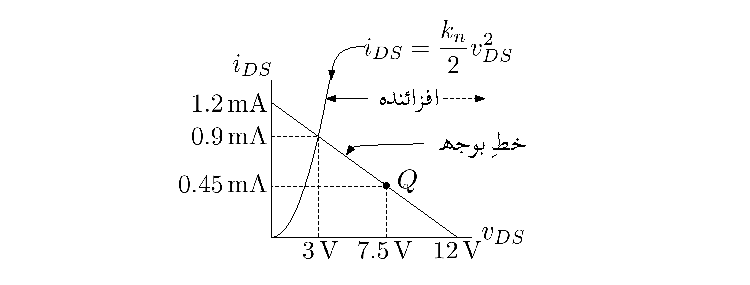
\includegraphics[scale=0.90]{mosfetLoadlineExampleA}
\caption{خطِ بوجھ سے نقطہ کارکردگی کا حصول }
\label{شکل_ماسفیٹ_بار_کا_خط_سے_نقطہ _کارکردگی_الف}
\end{figure}

ان دو مساوات کو اکٹھے کرتے  ہوئے
\begin{align*}
12&=v_{DS}+10000 i_{DS}\\
&=v_{DS}+10000 \times \frac{0.2 \times 10^{-3}}{2} v_{DS}^2
\end{align*}
حاصل ہوتا ہے۔اس دو درجی مساوات سے \عددی{v_{DS}=\SI{3}{\volt}} حاصل ہوتا ہے۔اس کا دوسرے جواب \عددی{\SI{-4.5}{\volt}} ہے جسے رد کیا جاتا ہے چونکہ \عددی{v_{DS}} منفی ممکن نہیں۔حاصل \عددی{v_{DS}} سے \عددی{i_{DS}=\SI{0.9}{\milli \ampere}} حاصل ہوتا ہے۔

ماسفیٹ ایمپلیفائر \اصطلاح {خطِ بوجھ} پر چہل قدمی کرتا ہے۔جیسے شکل میں دکھایا گیا ہے، ماسفیٹ اس وقت تک افزائندہ رہتا ہے جب تک \عددی{v_{DS}}  کی قیمت \عددی{v_{DSدبوچ}} سے زیادہ ہو۔یوں ماسفیٹ کا \عددی{v_{DS}} تین وولٹ سے کم نہیں رکھا جا سکتا لہٰذا
\begin{align*}
\SI{3}{\volt} \le v_{DS} < \SI{12}{\volt}\\
0 < i_{DS} < \SI{0.9}{\milli \ampere}
\end{align*}
خارجی متغیرات کے حدود ہیں جن میں ماسفیٹ افزائندہ رہے گا۔ان قیمتوں کے بالکل درمیانی نقطے پر نقطہ کارکردگی رکھنے سے زیادہ سے زیادہ \عددی{v_{DS}} اور \عددی{i_{DS}} حاصل کرنا ممکن ہو گا۔یوں نقطہ کارکردگی کو  \عددی{\left(\SI{7.5}{\volt},\SI{0.45}{\milli \ampere} \right)} رکھا جائے گا۔
\انتہا{مثال}
%===================
\ابتدا{مثال}
\عددی{p} بڑھاتا ماسفیٹ استعمال کرتے ہوئے شکل  \حوالہ{شکل_جمع_ماسفیٹ_کے_یک_سمتی_ادوار_الف} الف  کا دور بنایا گیا ہے۔ ماسفیٹ کو افزائندہ خطے میں رکھتے ہوئے \عددی{V_D=\SI{4}{\volt}} اور \عددی{I_{SD}=\SI{0.2}{\milli \ampere}} حاصل کریں۔

حل:\عددی{I_{SD}=\SI{0.2}{\milli \ampere}} اور \عددی{V_D=\SI{4}{\volt}} حاصل کرنے کی خاطر اُوہم کے قانون کے تحت
\begin{align*}
V_D&=I_{SD}R_D\\
4&=0.2 \times 10^{-3}R_D\\
R_D&=\SI{20}{\kilo \ohm}
\end{align*}
حاصل ہوتا ہے۔

افزائندہ ماسفیٹ کی مساوات سے
\begin{align*}
I_{SD}&=\frac{k_p}{2} \left(V_{SG}+V_t \right )^{2}\\
0.2 \times 10^{-3}&=\frac{0.1 \times 10^{-3}}{2} \left(V_{SG}-2 \right )^2 \\
V_{SG}&=\SI{0}{\volt}, \SI{4}{\volt}
\end{align*}
حاصل ہوتے ہیں۔افزائندہ \عددی{p} بڑھاتا ماسفیٹ کے لئے ضروری ہے کہ \عددی{{V_{SG}> -V_t}} رہے۔چونکہ
\begin{align*}
-V_t=-\left(-2 \right)=\SI{2}{volt}
\end{align*}
ہے لہٰذا اس شرط کا مطلب ہے کہ \عددی{V_{SG} > \SI{2}{\volt}} ہو۔یوں \عددی{V_{SG}=\SI{4}{\volt}}  کو درست جواب تسلیم کیا جاتا ہے۔یوں چونکہ \عددی{V_S=\SI{5}{\volt}} لہٰذا
\begin{align*}
V_{SG}&=V_S-V_G\\
4&=5-V_G\\
V_G&=\SI{1}{\volt}
\end{align*}
درکار ہے۔
\begin{figure}
\centering
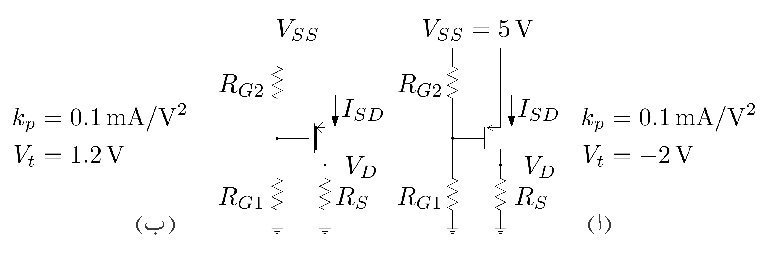
\includegraphics[scale=0.90]{pMosfetDCcircuitsA}
\caption{\عددی{p} ماسفیٹ کے یک سمتی ادوار}
\label{شکل_جمع_ماسفیٹ_کے_یک_سمتی_ادوار_الف}
\end{figure}
\عددی{R_{G1}} اور \عددی{R_{G2}} کے قیمتیں چن کر \عددی{V_G=\SI{1}{\volt}}  حاصل کیا جا سکتا ہے۔مثلاً اگر \عددی{R_{G1}=\SI{1}{\mega \ohm}} چنا جائے تو
\begin{align*}
V_G&=\frac{R_{G1} V_{SS}}{R_{G1}+R_{G2}}\\
R_{G2}&=R_{G1} \left(\frac{V_{SS}}{V_G}-1 \right )\\
R_{G2}&=\SI{4}{\mega \ohm}
\end{align*}
حاصل ہوتا ہے۔
\انتہا{مثال}
%=========

\ابتدا{مثال}
شکل \حوالہ{شکل_جمع_ماسفیٹ_کے_یک_سمتی_ادوار_الف} ب میں \عددی{p} قسم کا گھٹاتا ماسفیٹ استعمال کرتے دور بنایا گیا ہے جس میں ماسفیٹ کو افزائندہ رکھتے ہوئے  \عددی{V_D=\SI{1}{\volt}} اور
  \عددی{I_{SD}=\SI{0.2}{\milli \ampere}} درکار ہیں۔ اس دور کو حل کریں۔

حل:	اُوہم کے قانون کے تحت
\begin{align*}
V_D=I_{SD}R_D\\
1=0.2 \times 10^{-3} R_D\\
R_D=\SI{5}{\kilo \ohm}
\end{align*}
افزائندہ ماسفیٹ کی مساوات سے
\begin{align*}
I_{SD}=\frac{k_p}{2} \left(V_{SG}+V_t \right )^{2} \\
0.2 \times 10^{-3}=\frac{0.1 \times 10^{-3}}{2} \left(V_{SG}+1.2 \right )^{2}\\
V_{SG}=\SI{-3.2}{\volt}, \SI{0.8}{\volt}
\end{align*}
چالو \عددی{p}  قسم کے گھٹاتا ماسفیٹ کے لئے \عددی{V_{SG} >-V_t} یعنی \عددی{V_{SG}> \SI{-1.2}{\volt}} ضروری ہے ۔یوں \عددی{V_{SG}=\SI{-3.2}{\volt}}  کو رد کیا جاتا ہے اور   \عددی{V_{SG}=\SI{0.8}{\volt}} کو درست جواب تسلیم کیا جاتا ہے۔یوں
\begin{align*}
V_{SG}=V_S-V_G\\
0.8=5-V_G\\
V_G=\SI{4.2}{\volt}
\end{align*}
درکار ہے۔ \عددی{R_{G1}=\SI{10}{\mega \ohm}} لیتے ہوئے
\begin{align*}
R_{G2}=R_{G1} \left(\frac{V_{SS}}{V_G}-1 \right )=10 \times 10^{6} \left(\frac{5}{4.2}-1 \right)=\SI{1.9}{\mega \ohm}
\end{align*}
حاصل ہوتا ہے۔

\انتہا{مثال}
%========

\ابتدا{مثال}
شکل \حوالہ{شکل_ماسفیٹ_کے_یک_سمتی_ادوار_پ} الف میں \عددی{I_{DS}} اور \عددی{V_{DS}} حاصل کریں۔گھٹاتا ماسفیٹ کے
\begin{align*}
k_n&=\SI{0.1}{\milli \ampere \volt^{-2}}\\
V_t&=\SI{-1}{\volt}
\end{align*}
ہیں۔

حل:	ماسفیٹ کا گیٹ برقی زمین پر ہے یعنی \عددیء{V_G=\SI{0}{\volt}} ہے۔بقایا دو سروں کے لئے ہم لکھ سکتے ہیں۔
\begin{align*}
V_S=I_{DS}R_S =2000I_{DS}\\
V_D=V_{DD}-I_{DS}R_D=5-16000 I_{DS}
\end{align*}
یوں
\begin{align*}
V_{GS}=V_G-V_S=0-2000I_{DS}=-2000I_{DS}
\end{align*}
تصور کرتے ہیں کہ ماسفیٹ افزائندہ ہے۔اس طرح
\begin{align*}
I_{DS}=\frac{k_n}{2}\left(V_{GS}-V_t \right )^2 \\
I_{DS}=\frac{0.1 \times 10^{-3}}{2} \left[\left(-2000I_{DS} \right )-(-1) \right ]^2 \\
I_{DS}=\SI{5.958}{\milli \ampere}, \SI{0.042}{\milli \ampere}
\end{align*}
 \عددی{\SI{5.958}{\milli \ampere}} کے برقی رو سے  \عددی{V_{GS}=-5.958 \times 10^{-3} \times 2000=\SI{-11.9}{\volt}} حاصل ہوتا ہے جو کہ منقطع ماسفیٹ کی نشانی ہے لہٰذا اس جواب کو رد کیا جاتا ہے۔ \عددی{\SI{0.042}{\milli \ampere}} کے برقی رو سے \عددی{V_{GS}=-0.042 \times 10^{-3} \times 2000=\SI{-0.084}{\volt}} حاصل ہوتا ہے جو کہ چالو ماسفیٹ کی نشانی ہے۔یہی صحیح جواب ہے۔مزید یہ کہ
\begin{align*}
V_S=0.042 \times 10^{-3} \times 2000=\SI{0.084}{\volt}\\
V_D=5-0.042 \times 10^{-3} \times 16000=\SI{4.328}{\volt}\\
V_{DS}=V_D-V_S=4.328-0.084=\SI{4.224}{ \volt}\\
V_{GD}=V_G-V_D=0-4.328=\SI{-4.328}{\volt}
\end{align*}
چونکہ  \عددی{V_{GD}<V_t} ہے لہٰذا ماسفیٹ افزائندہ ہی ہے جیسے تصور کیا گیا تھا۔
\begin{figure}
\centering
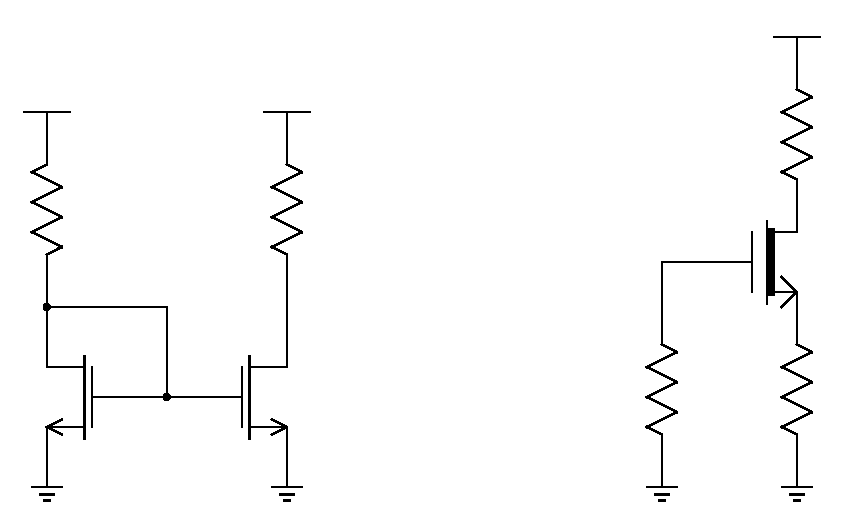
\includegraphics[scale=0.90]{mosfetDCcircuitsC}
\caption{ماسفیٹ کے یک سمتی ادوار}
\label{شکل_ماسفیٹ_کے_یک_سمتی_ادوار_پ}
\end{figure}
\انتہا{مثال}
%=====

\ابتدا{مثال}
شکل \حوالہ{شکل_ماسفیٹ_کے_یک_سمتی_ادوار_پ} ب میں \اصطلاح {برقی آئینہ}\فرہنگ{آئینہ}\فرہنگ{mirror}\حاشیہب{mirror}  دکھایا گیا ہے۔اس دور میں استعمال ہونے والے دونوں ماسفیٹ کو بالکل یکساں تصور کرتے ہوئے اسے حل کریں۔

حل: \عددی{Q_1} کا گیٹ اس کے ڈرین کے ساتھ منسلک کیا گیا ہے۔یہاں رک کر مثال \حوالہ{مثال_میدانی_گیٹ_اور_محاصل_جڑے}  کو دوبارہ دیکھیں جہاں اس طرح جڑے ماسفیٹ پر تفصیلی گفتگو کی گئی ہے۔

ماسفیٹ کا گیٹ اور ڈرین جڑے ہونے کی وجہ سے ان دونوں پر برابر برقی دباو پایا جائے گا یعنی \عددی{V_{G1}=V_{D1}} ہو گا۔یوں \عددی{V_{GS1}=V_{DS1}} اور  \عددی{V_{GS1}-V_{DS1}<V_t} ہو گا۔یہ افزائندہ ماسفیٹ کی نشانی ہے۔

کرچاف کے قانون برائے برقی دباو کے تحت
\begin{align*}
V_{DD}=I_{DS1}R_1+V_{DS1}\\
V_{DS1}=V_{DD}-I_{DS1}R_1
\end{align*}
ہے۔چونکہ \عددی{V_{DS1}} اور \عددی{V_{GS1}} برابر ہیں لہٰذا
\begin{align*}
V_{GS1}=V_{DS1}=V_{DD}-I_{DS1}R_1
\end{align*}
ہو گا اور یوں
\begin{align*}
I_{DS1}&=\frac{k_n}{2}\left(V_{GS}-V_t \right )^2 \\
&=\frac{k_n}{2} \left[\left(V_{DD}-I_{DS1} R_1 \right )-V_t \right ]^{2}
\end{align*}
ہو گا۔اس مساوات کو حل کرتے برقی رو کی دو مقداریں حاصل ہوں گے جن میں سے صرف ایک مقدار قابلِ قبول ہو گی۔اس برقی رو کے مطابق \عددی{V_{GS1}} حاصل کیا جا سکتا ہے۔

دور میں دونوں ماسفیٹ کے گیٹ آپس میں جڑے ہیں جبکہ دونوں کے سورس برقی زمین پر ہیں۔یوں \عددی{V_{GS2}=V_{GS1}} ہو گا۔جب تک ماسفیٹ \عددی{Q_2} بھی افزائندہ رہے اس کی برقی رو
\begin{align*}
I_{DS2}=\frac{k_n}{2} \left(V_{GS2}-V_t \right )^2
\end{align*}
ہو گی جو کہ ماسفیٹ \عددی{Q_1} کے برقی رو کے برابر ہے یعنی \عددی{I_{DS2}=I_{DS1}} ۔یوں \عددی{R_1}  کی مدد سے \عددی{Q_1}  میں درکار برقی رو حاصل کی جاتی ہے۔چونکہ  \عددی{V_{GS1}} اور \عددی{V_{GS2}} برابر ہیں لہٰذا \عددی{Q_2} میں بھی \عددی{Q_1} کے برقی رو جتنا برقی رو گزرے گا۔

\انتہا{مثال}

%=========
\حصہ{ماسفیٹ ایمپلیفائر کا ترسیمی تجزیہ}
ماسفیٹ کو بطور ایمپلیفائر استعمال کر نے کی خاطر اسے افزائندہ خطے میں مائل کیا جاتا ہے۔شکل \حوالہ{شکل_ماسفیٹ_ایمپلیفائر_ترسیمی_تجزیہ} میں ماسفیٹ ایمپلیفائر دکھایا گیا ہے۔ساتھ ہی ماسفیٹ کے خطوط اور برقی خطِ بوجھ بھی دکھایا گیا ہے۔افزائندہ خطے کے حد کو \عددی{v_{DS\textrm{دبوچ}}} کے خط سے دکھایا گیا ہے۔ماسفیٹ ایمپلیفائر اس وقت تک خوش اسلوبی سے داخلی اشارے کو بڑھاتا ہے جب تک ماسفیٹ افزائندہ خطے میں رہے۔ہم یہاں \تحریر{nMOSFET} کو مثال بنا کر ماسفیٹ ایمپلیفائر پر تبصرہ کریں گے۔ماسفیٹ کے بقایا تمام اقسام پر مبنی ایمپلیفائر بھی اسی طرح کام کرتے ہیں۔
\begin{figure}
\centering
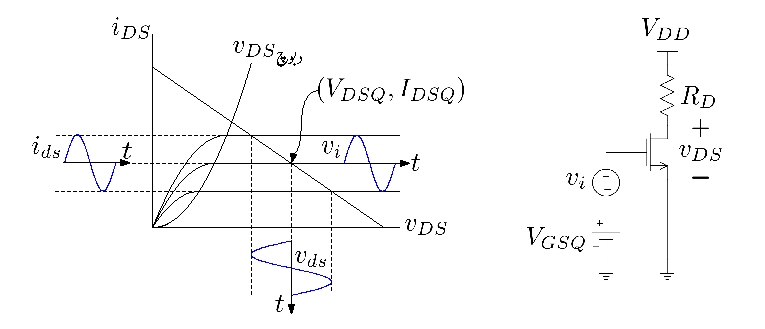
\includegraphics[scale=0.90]{nEnhancementGraphicalA}
\caption{ماسفیٹ ایمپلیفائر}
\label{شکل_ماسفیٹ_ایمپلیفائر_ترسیمی_تجزیہ}
\end{figure}

شکل \حوالہ{شکل_ماسفیٹ_ایمپلیفائر_ترسیمی_تجزیہ} میں نقطہ کارکردگی ماسفیٹ کے گیٹ پر برقی دباو \عددیء{V_{GSQ}}، بوجھ کی مزاحمت \عددی{R_D} اور برقی دباو کی منبع \عددی{V_{DD}} تعین کرتے ہیں۔\عددی{v_i=0} ہونے کی صورت میں ماسفیٹ نقطہ کارکردگی پر پایا جائے گا جہاں اس کے یک سمتی برقی دباو \عددیء{V_{DSQ}} اور یک سمتی برقی رو \عددی{I_{DSQ}} ہوں گے۔اب تصور کریں کہ باریک اشارہ \عددی{v_i} مثبت جانب بڑھتا ہے۔یوں ماسفیٹ کے گیٹ پر کل برقی دباو \عددی{V_{GSQ}} سے بڑھ جائے گا جس سے  \عددی{i_{DS}} بڑھ جائے گی جبکہ \عددی{v_{DS}} گھٹ جائے گا۔اسی طرح اگر \عددی{v_i} منفی ہوتا ہے تو گیٹ پر برقی دباو گھٹے گا جس سے \عددی{i_{DS}} گھٹے گی جبکہ \عددی{v_{DS}} بڑھے گا۔شکل میں سائن نما \عددی{v_i} کی صورت میں ایسا ہوتا دکھایا گیا ہے۔آپ دیکھ سکتے ہیں کہ خطِ بوجھ کی ڈھلوان کم کرنے سے \عددی{v_{ds}} بڑھتا ہے۔\عددی{\tfrac{v_{ds}}{v_i}} اس ایمپلیفائر کی افزائش برقی دباو \عددی{A_v} ہے۔

\حصہ{ماسفیٹ ایمپلیفائر کا تحلیلی تجزیہ}
شکل \حوالہ{شکل_ماسفیٹ_ایمپلیفائر_الف}  میں بڑھاتا ماسفیٹ کو استعمال کرتے ہوئے ایمپلیفائر کا دور بنایا گیا ہے جس میں دو عدد منبع برقی دباو \عددی{V_{DD}}  اور \عددی{V_{GS}} ماسفیٹ کو مائل کرنے کی خاطر استعمال کئے گئے ہیں۔جیسا کہ ہم اسی باب میں آگے دیکھیں گے، حقیقت میں عموماً ایسا نہیں کیا جاتا۔بہر حال اس دور کی مدد سے ایمپلیفائر پر غور کرنا نسبتاً آسان ہے۔

اس دور میں داخلی جانب یک سمتی منبع \عددی{V_{GS}} کے ساتھ سلسلہ وار بدلتا اشارہ \عددی{v_{gs}} منسلک کیا گیا ہے۔اس دور کا مقصد داخلی اشارہ \عددی{v_{gs}} کا حیطہ بڑھانا ہے۔بڑھایا گیا اشارہ ماسفیٹ کے ڈرین سے حاصل کیا جائے گا۔

مندرجہ ذیل بحث گزشتہ باب میں ٹرانزسٹر پر بحث کے ہو بہو ہے۔

\جزوحصہ{یک سمتی تجزیہ}
 ماسفیٹ کا نقطہ کارکردگی حاصل کرنے کی خاطر بدلتے اشارہ کو قصر دور کیا جاتا ہے یعنی اس کی قیمت صفر کر دی جاتی ہے۔یوں
\begin{align} \label{مساوات_میدانی_یکسمتی_رو}
I_{DS}=\frac{k_n}{2} \left(V_{GS}-V_t \right )^2
\end{align}
حاصل ہوتا ہے۔خارجی جانب کرچاف کے قانون برائے برقی دباو سے
\begin{align} \label{مساوات_میدانی_یکسمتی_خارجی_دباو}
V_{DS}=V_{DD}-I_{DS}R_D
\end{align}
حاصل ہوتا ہے۔ماسفیٹ افزائندہ رہنے کی خاطر
\begin{align*}
V_{GS}-V_{DS}<V_t
\end{align*}
کا ہونا ضروری ہے۔
\جزوحصہ{بدلتی رو تجزیہ}
بدلتی رو تجزیہ کی خاطر دور میں \عددی{v_{gs}} پر نظر رکھی جائے گی۔شکل \حوالہ{شکل_ماسفیٹ_ایمپلیفائر_الف}  میں  \عددی{V_{GS}} اور \عددی{v_{gs}} سلسلہ وار جوڑنے سے
\begin{align}
v_{GS}=V_{GS}+v_{gs}
\end{align}
%
\begin{figure}
\centering
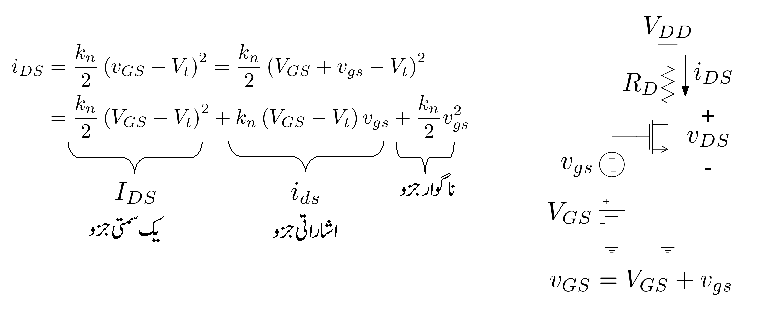
\includegraphics[scale=0.90]{enhancementNmosfetAmplifierA}
\caption{ماسفیٹ ایمپلیفائر کے برقی رو کے مختلف اجزاء}
\label{شکل_ماسفیٹ_ایمپلیفائر_الف}
\end{figure}
حاصل ہوتا ہے جس کو استعمال کرتے ہوئے

\begin{align}\label{شناخت_مساوات_ماسفیٹ_خط_کی_مساوات_بدلتی_رو}
i_{DS}=\frac{k_n}{2} \left(v_{GS}-V_t \right)^2
\end{align}
سے
\begin{gather} \label{مساوات_میدانی_رو_کے_حصے}
\begin{aligned}
i_{DS}&=\frac{k_n}{2} \left(V_{GS}+v_{gs}-V_t \right )^2\\
&=\frac{k_n}{2}\left[\left(V_{GS}-V_t\right)+v_{gs} \right ]^2\\
&=\frac{k_n}{2} \left[\left(V_{GS}-V_t \right )^2+2 \left(V_{GS}-V_t \right ) v_{gs}+v_{gs}^{2} \right ] \\
&=\frac{k_n}{2} \left(V_{GS}-V_t \right )^2+k_n \left(V_{GS}-V_t \right ) v_{gs}+ \frac{k_n}{2} v_{gs}^{2} 
\end{aligned}
\end{gather}
حاصل ہوتا ہے۔اس مساوات کا پہلا جزو \عددی{\frac{k_n}{2}\left(V_{GS}-V_t \right )^2}   یک سمتی جزو ہے۔ یہ مساوات \حوالہ{مساوات_میدانی_یکسمتی_رو}  میں دئے  \عددی{I_{DS}} کے برابر ہے اور یوں اسے \عددی{I_{DS}} لکھا جا سکتا ہے۔مساوات کا دوسرا جزو \عددی{k_n \left(V_{GS}-V_t \right) v_{gs} }  بدلتی رو جزو ہے۔یہ جزو داخلی اشارہ کا  \عددی{k_n \left (V_{GS}-V_t \right )} گنّا بڑھایا جزو ہے اور یوں اسے \عددی{i_{ds}}  لکھا جا سکتا ہے۔مساوات کا تیسرا جزو \عددی{v_{gs}} کے مربع کے راست تناسب ہے اور یوں یہ جزو اشارہ کی \اصطلاح {شکل بگاڑتا}\فرہنگ{شکل بگاڑنا}\فرہنگ{distortion}\حاشیہب{distortion}  ہے۔یہ آخری جزو  \عددی{ \frac{k_n}{2}v_{gs}^2} نا گوارہ جزو ہے۔اشارہ کی اصل شکل برقرار رکھنے کی خاطر اس جزو کی قیمت دوسرے جزو سے بہت کم رکھنی ضروری ہے یعنی
\begin{align*}
\frac{k_n}{2}v_{gs}^2 \ll k_n \left(V_{GS}-V_t \right )v_{gs}
\end{align*}
اس سے حاصل ہوتا ہے
\begin{align} \label{مساوات_میدانی_باریک_اشارہ_کی_شرط}
v_{gs} \ll 2 \left(V_{GS}-V_t \right )
\end{align}
مساوات \حوالہ{مساوات_میدانی_باریک_اشارہ_کی_شرط}   \اصطلاح {باریک اشارہ}\حاشیہب{small signal}  کی شرط بیان کرتا ہے۔جو اشارہ اس مساوات پر پورا اترے اسے \اصطلاح {باریک اشارہ} تصور کیا جاتا ہے۔

اگر داخلی اشارہ باریک اشارہ کی شرط پر پورا  اترے تب مساوات \حوالہ{مساوات_میدانی_رو_کے_حصے} میں آخری جزو کو نظر انداز یا جا سکتا ہے اور اسے یوں لکھا جا سکتا ہے۔
\begin{align} \label{مساوات_میدانی_یکسمتی_اور_بدلتی_رو}
i_{DS} \approx I_{DS} +i_{ds}
\end{align}
جہاں
\begin{align} \label{مساوات_میدانی_باریک_رو_الف}
i_{ds}=k_n \left(V_{GS}-V_t \right )v_{gs}
\end{align}
مساوات \حوالہ{مساوات_میدانی_باریک_رو_الف}  کو یوں بھی لکھا جا سکتا ہے۔
\begin{align} \label{مساوات_میدانی_خارجی_رو_بالمقابل_داخلی_دباو}
i_d=g_m v_{gs}
\end{align}
جہاں
\begin{align} \label{مساوات_میدانی_موصلیت_نما_بطور_افزائش}
g_m =\frac{i_d}{v_{gs}}=k_n \left(V_{GS}-V_t \right )
\end{align}
ماسفیٹ کی باریک اشاراتی موصل-نما افزائش ہے۔مساوات \حوالہ{مساوات_میدانی_یکسمتی_رو} کی مدد سے \عددی{g_m} کو یوں بھی لکھا جا سکتا ہے۔
\begin{gather}
\begin{aligned}\label{مساوات_ماسفیٹ_باریک_افزائش_کے_مختلف_مساوات}
g_m&=\sqrt{2 I_{DS} k_n}\\
&=\frac{2 I_{DS}}{V_{GS}-V_t}
\end{aligned}
\end{gather}

\عددی{g_m} کے با ضابطہ تعریف کے مطابق یہ ماسفیٹ کے  \عددی{i_{DS}-v_{GS}} خط کے نقطہ مائل پر مماس کی ڈھلوان ہے یعنی
\begin{align}\label{مساوات_ماسفیٹ_افزائش_کا_جزوی_تفرق_سے_حصول}
g_m =\left. \frac{\partial i_{DS}}{\partial v_{GS}} \right |_{v_{GS}=V_{GSQ}}
\end{align}

اشارہ \عددی{v_{gs}} کی موجودگی میں مساوات \حوالہ{مساوات_میدانی_یکسمتی_خارجی_دباو}  مندرجہ ذیل صورت اختیار کر لیتا ہے۔
\begin{align}
v_{DS}=V_{DD}-i_{DS}R_D
\end{align}
مساوات  \حوالہ{مساوات_میدانی_یکسمتی_اور_بدلتی_رو} کے استعمال سے 
\begin{gather}
\begin{aligned}
v_{DS}&=V_{DD}-\left(I_{DS}+i_{ds} \right )R_D\\
&=V_{DD}-I_{DS}R_D-i_{ds}R_D
\end{aligned}
\end{gather}
یہ مساوات داخلی اشارہ کے موجودگی میں خارجی برقی دباو دیتا ہے۔داخلی اشارہ کے عدم موجودگی میں \عددی{i_{ds}} کی قیمت صفر ہو گی اور اس سے مساوات \حوالہ{مساوات_میدانی_یکسمتی_خارجی_دباو} حاصل ہو گا۔اس مساوات کو یوں بھی لکھا جا سکتا ہے۔
\begin{align}
v_{DS}=V_{DS}+v_{ds}
\end{align}
جہاں \عددی{V_{DS}}  مساوات \حوالہ{مساوات_میدانی_یکسمتی_خارجی_دباو}  میں دی گئی ہے جبکہ 
\begin{align}
v_{ds}=-i_{ds} R_D
\end{align}
ہے۔مساوات \حوالہ{مساوات_میدانی_خارجی_رو_بالمقابل_داخلی_دباو}  کی مدد سے
\begin{align}
v_{ds}=-g_m R_D v_{gs}
\end{align}
حاصل ہوتا ہے جس سے افزائش برقی دباو یوں حاصل ہوتا ہے۔
\begin{align}\label{مساوات_ماسفیٹ_افزائش_کی_سادہ_مساوات}
A_v=\frac{v_{ds}}{v_{gs}}=-g_m R_D
\end{align}
یہاں منفی علامت کا مطلب یہ ہے کہ جب داخلی اشارہ \عددی{v_{gs}}  مثبت ہو تب خارجی اشارہ  \عددی{v_{ds}} منفی ہو گا یعنی یہ دو اشارات آپس میں \عددی{\SI{180}{\degree}}  زاویہ پر رہتے ہیں۔

شکل \حوالہ{شکل_ماسفیٹ_ایمپلیفائر_گیٹ_دباو_بالمقابل_برقی_رو} میں  مساوات \حوالہ{شناخت_مساوات_ماسفیٹ_خط_کی_مساوات_بدلتی_رو} کا خط کھینچا گیا ہے۔نقطہ  کارکردگی پر اس خط کی ڈھلون \عددی{g_m} کہلاتی ہے۔داخلی اشارہ \عددی{v_{gs}} کے عدم موجودگی میں ماسفیٹ نقطہ کارکردگی \عددی{Q} پر رہے گا اور یوں اس پر \عددی{V_{GSQ}} اور \عددی{I_{DSQ}} پائے جائیں گے۔سائن نما \عددی{v_{gs}} کی صورت میں \عددی{i_{DS}} میں سائن نما جزو پایا جائے گا جسے \عددی{i_{ds}} کہا جاتا ہے۔
\begin{figure}
\centering
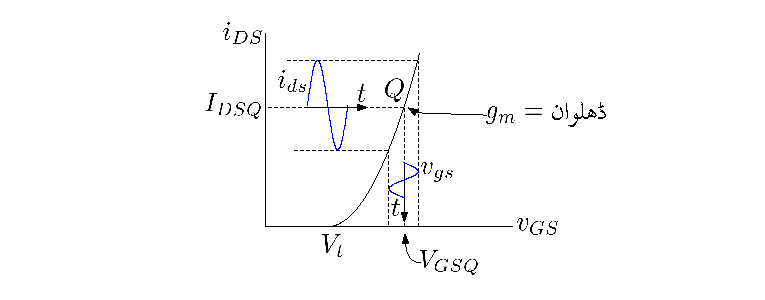
\includegraphics[scale=0.90]{mosfetGateVersusCurrent}
\caption{ماسفیٹ ایمپلیفائر کا گیٹ پر برقی دباو بالمقابل ماسفیٹ کی برقی رو کا خط}
\label{شکل_ماسفیٹ_ایمپلیفائر_گیٹ_دباو_بالمقابل_برقی_رو}
\end{figure}
%===================
\حصہ{ماسفیٹ ماڈل}
اس حصے میں ماسفیٹ کے ماڈل حاصل کئے جائیں گے جنہیں استعمال کر کے بدلتے برقی دباو اور بدلتے برقی رو حاصل کئے جاتے ہیں۔
\جزوحصہ{خارجی مزاحمت  \عددی{r_o}}

ماسفیٹ کو بطورِ ایمپلیفائر استعمال کرنے کی خاطر اسے افزائندہ خطے میں مائل کیا جاتا ہے۔مساوات \حوالہ{مساوات_میدانی_نقطہ _دبوچ_رو}  کے مطابق افزائندہ خطے میں \عددی{v_{DS}} تبدیل کرنے سے \عددی{i_{DS}} پر کوئی اثر نہیں ہوتا۔صفحہ \pageref{شکل_بڑھاتے_ماسفیٹ_کے_خط_منفی}  پر شکل \حوالہ{شکل_بڑھاتے_ماسفیٹ_کے_خط_منفی} پ میں  \عددی{v_{DS}} کو \زیرنوشت{v}{DS}{دبوچ} سے بڑھانے پر پیدا کردہ راہ کی لمبائی کم ہوتے دکھائی گئی ہے۔مساوات \حوالہ{مساوات_میدانی_نقطہ _دبوچ_رو}  حاصل کرتے وقت اس اثر کو نظر انداز کیا گیا۔پیدا کردہ راہ کی لمبائی کم ہونے سے پیدا کردہ راہ کی مزاحمت کم ہو جاتی ہے اور یوں \عددی{i_{DS}} بڑھ جاتا ہے۔بڑھتے برقی دباو کے ساتھ پیدا کردہ راہ کی لمبائی کم ہونے کے اثر کو ہم مساوات  \حوالہ{مساوات_میدانی_نقطہ _دبوچ_رو} میں \اصطلاح {ارلی برقی دباو}\فرہنگ{ارلی برقی دباو}\فرہنگ{Early voltage}\حاشیہب{Early voltage} \عددی{V_A}  کے طرز کا جزو شامل کرنے سے حاصل کر سکتے ہیں جیسے
\begin{gather}
\begin{aligned}
i_{DS}&=\frac{k_n'}{2} \left[\frac{W}{L} \right ] \left[v_{GS}-V_t \right ]^{2} \left [1+\frac{v_{DS}}{V_A} \right ]\\
&=\frac{k_n}{2} \left[v_{GS}-V_t \right ]^{2} \left [1+\frac{v_{DS}}{V_A} \right ]
\end{aligned}
\end{gather}
%
\begin{figure}
\centering
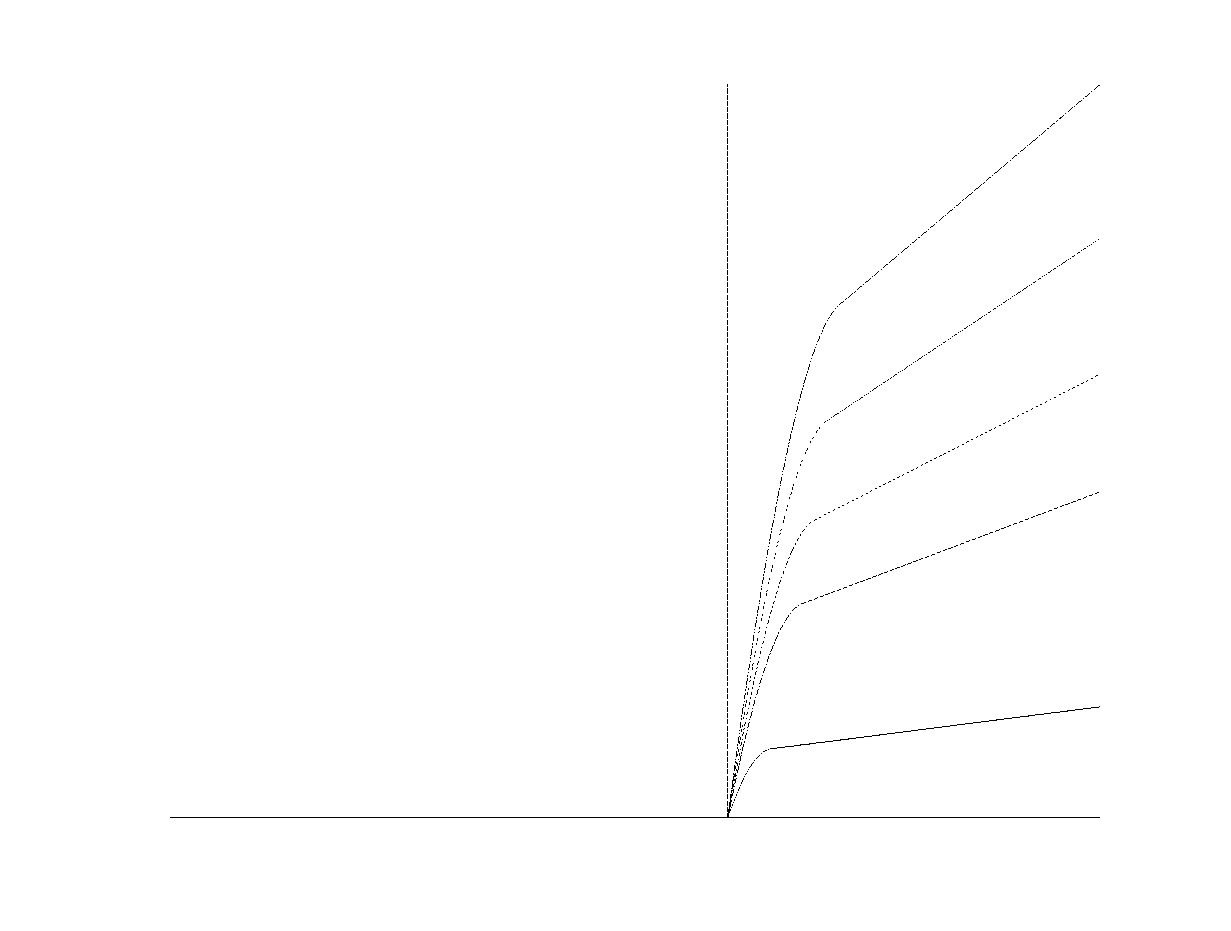
\includegraphics[scale=0.90]{nEnhancementCharacteristicsEarlyVoltage}
\caption{ارلی برقی دباو}
\label{شکل_ماسفیٹ_ارلی_برقی_دباو}
\end{figure}

\اصطلاح {ارلی برقی دباو} کے اثر کو شامل کرتے ہوئے ماسفیٹ کے خط شکل \حوالہ{شکل_ماسفیٹ_ارلی_برقی_دباو} میں گراف کئے گئے ہیں۔اس مساوات سے ماسفیٹ کا خارجی مزاحمت حاصل کرنے کی غرض سے اس کا تفرق نقطہ مائل پر لیتے ہیں۔
\begin{align*}
\left . \frac{\partial i_{DS}}{\partial v_{DS}}  \right  |_{V_{GS}} = \frac{k_n}{2} \left(V_{GS}-V_t  \right)^2  \frac{1}{V_A}
\end{align*}
اور یوں 
\begin{align}
r_o=\left. \frac{\partial i_{DS}}{\partial v_{DS}} \right |_{v_{GS}}^{-1}=\frac{1}{\frac{k_n}{2} \left[v_{GS}-V_t \right ]^2 \frac{1}{V_A}}
\end{align}
حاصل ہوتا ہے۔اگر ارلی برقی دباو کے اثر کو نظر انداز کیا جائے تو \عددی{\frac{k_n}{2} \left(v_{GS}-V_t \right )^2} کو \عددی{I_{DS}} لکھا جا سکتا ہے اور یوں مندرجہ بالا خارجی مزاحمت کی مساوات کو بہتر طریقے سے یوں لکھا جا سکتا ہے۔
\begin{align} \label{مساوات_میدانی_خارجی_مزاحمت}
r_o=\left. \frac{\partial i_{DS}}{\partial v_{DS}} \right |_{v_{GS}}^{-1} \approx \frac{V_A}{I_{DS}}
\end{align}
ہم \عددی{V_A} کو \اصطلاح {ارلی برقی دباو} ہی کہیں گے۔\اصطلاح {ارلی برقی دباو} کی قیمت پیدا کردہ راہ کے لمبائی کے  راست تناسب ہوتا ہے۔
\begin{align}
V_A \propto L_{\textrm{راہ}}
\end{align}
یوں \عددی{r_o} بڑھانے کی خاطر زیادہ لمبائی کی راہ تخلیق دی جاتی ہے۔ماسفیٹ کے ارلی برقی دباو کی عمومی قیمت \عددی{\SI{200}{\volt}} تا \عددی{\SI{300}{\volt}} ہوتی ہے۔

\جزوحصہ{وسیع اشاراتی ماسفیٹ ماڈل}
افزائندہ خطے میں ماسفیٹ کا وسیع اشاراتی ماڈل شکل \حوالہ{شکل_وسیع_اشارات_ماسفیٹ_ماڈل}  میں دکھایا گیا ہے۔اس ماڈل کے داخلی جانب مزاحمت لامحدود ہے جبکہ مساوات \حوالہ{مساوات_میدانی_خارجی_مزاحمت}  اس کا خارجی مزاحمت \عددی{r_o}  دیتا ہے۔آپ دیکھ سکتے ہیں کہ اس ماڈل سے درست \عددی{i_{DS}}  حاصل ہوتا ہے۔
\begin{figure}
\centering
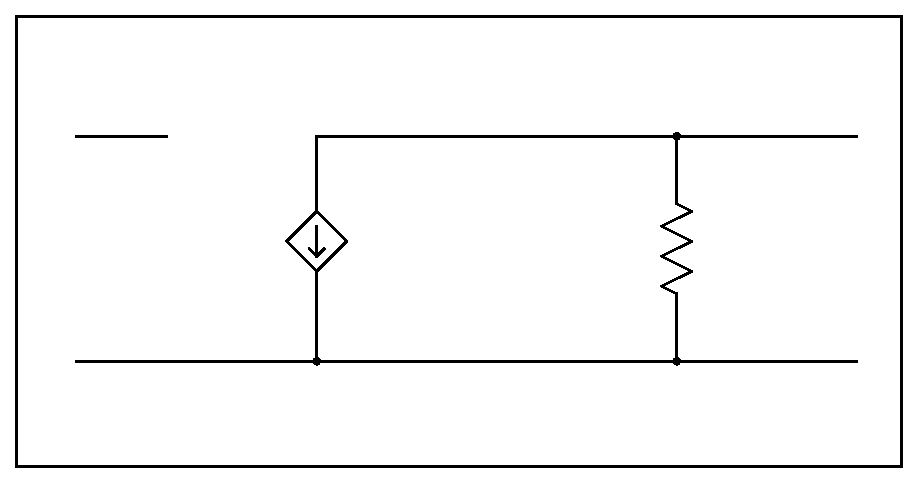
\includegraphics[scale=0.90]{MOSFETlargeSignalModel}
\caption{وسیع اشارات ماسفیٹ ماڈل}
\label{شکل_وسیع_اشارات_ماسفیٹ_ماڈل}
\end{figure}

\جزوحصہ{باریک اشاراتی ماسفیٹ \عددی{\pi} ماڈل}
ماسفیٹ کا باریک اشاراتی ماڈل بالکل \عددی{BJT} ٹرانزسٹر کی طرح حاصل کیا جاتا ہے۔افزائندہ خطے میں استعمال ہوتے ماسفیٹ کا باریک اشاراتی ماڈل حاصل کرنے کی غرض سے مساوات \حوالہ{مساوات_میدانی_افزائندہ_رو}  کا جزوی تفرق حاصل کرتے ہیں جس سے افزائش \عددی{g_m} حاصل ہو گی۔جزوی تفرق کی قیمت نقطہ مائل \عددی{V_{GS}} پر حاصل کیا جاتا ہے۔یوں
\begin{align} \label{مساوات_میدانی_موصلیت_نما}
g_m = \left. \frac{\partial i_{DS}}{\partial v_{GS}} \right |_{V_{GS}}=k_n \left[V_{GS}-V_t \right ]
\end{align}
حاصل ہوتا ہے۔مساوات \حوالہ{مساوات_میدانی_افزائندہ_رو}  کی یک سمتی شکل
\begin{align*}
I_{DS}=\frac{k_n}{2}\left(V_{GS}-V_t \right)^2
\end{align*}
سے
\begin{align*}
V_{GS}-V_t=\sqrt{\frac{2 I_{DS}}{k_n}}
\end{align*}
حاصل ہوتا ہے جس کی مدد سے مساوات \حوالہ{مساوات_میدانی_موصلیت_نما} کو  یوں بھی لکھا جا سکتا ہے۔
\begin{align} \label{مساوات_میدانی_موصلیت_نما_الف}
g_m=k_n \left[V_{GS}-V_t \right ]=k_n \sqrt{\frac{2 I_{DS}}{k_n}}=\sqrt{2 k_n I_{DS}}
\end{align}
مساوات \حوالہ{مساوات_میدانی_خارجی_مزاحمت}  سے حاصل  \عددی{r_o} اور مساوات \حوالہ{مساوات_میدانی_موصلیت_نما_الف}  سے حاصل  \عددی{g_m} استعمال کرتے ہوئے ماسفیٹ کا \اصطلاح {پست تعددی باریک اشاراتی ماسفیٹ پائے ماڈل} حاصل ہوتا ہے جسے شکل \حوالہ{شکل_باریک_اشاراتی_ماسفیٹ_ماڈل}  میں دائیں ہاتھ دکھایا گیا ہے۔اس ماڈل کا عمومی نام \عددی{\pi}  ماڈل ہے۔ دو جوڑ ٹرانزسٹر کے باریک اشاراتی ماڈل کے ساتھ موازنہ کرتے ہوئے صاف ظاہر ہے کہ ماسفیٹ کا داخلی مزاحمت لامحدود ہونے کی وجہ سے اس کی داخلی برقی رو صفر ہو گی۔
\begin{figure}
\centering
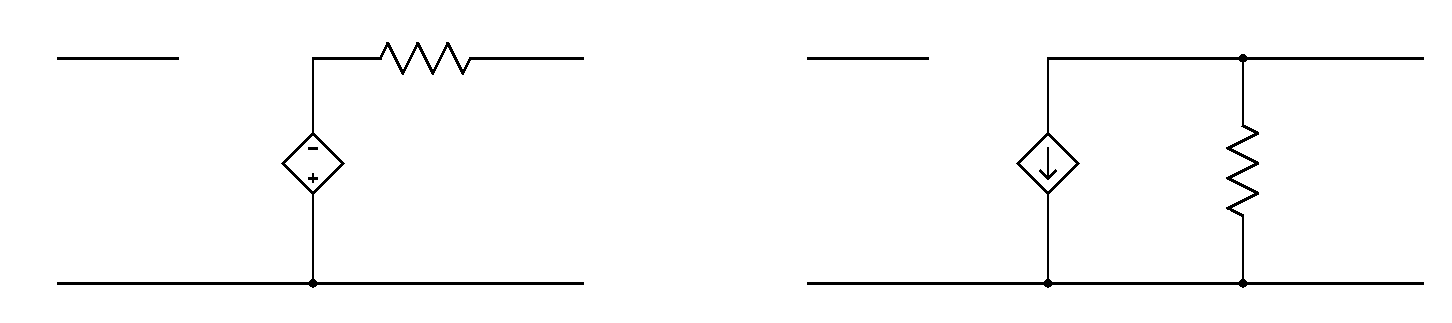
\includegraphics[scale=0.90]{MOSFETsmallSignalModelA}
\caption{پست تعددی باریک اشاراتی ماسفیٹ پائے ماڈل}
\label{شکل_باریک_اشاراتی_ماسفیٹ_ماڈل}
\end{figure}
ماسفیٹ کے \عددی{g_m} کا دو جوڑ ٹرانزسٹر کے  \عددی{g_m}  کے ساتھ موازنہ کرنے سے معلوم ہوتا ہے کہ ماسفیٹ کی برقی رو چار گنا کرنے سے اس کا   \عددی{g_m} دگنا ہوتا ہے جبکہ دو جوڑ ٹرانزسٹر کی برقی رو صرف دگنا کرنے سے ہی اس کا \عددی{g_m} دگنا ہو جاتا ہے۔

شکل \حوالہ{شکل_باریک_اشاراتی_ماسفیٹ_ماڈل} میں اسی ماڈل کی دوسری شکل بھی دکھائی گئی ہے جہاں ماڈل میں خارجی جانب نارٹن مساوی کی جگہ تھونن مساوی استعمال کیا گیا ہے۔یوں تھونن برقی دباو \عددی{g_m v_{gs} r_o} کے برابر لیتے ہوئے
\begin{align*}
\mu=g_m r_o
\end{align*} 
حاصل ہوتا ہے۔

ماسفیٹ کے گیٹ اور سورس کے مابین \عددی{C_{gs}} کپیسٹر پایا جاتا ہے۔اسی طرح گیٹ اور ڈرین کے مابین \عددی{C_{gd}} کپیسٹر پایا جاتا ہے۔کم تعدد پر ان کپیسٹر کو نظرانداز کیا جاتا ہے البتہ بلند تعدد پر ان کو نظرانداز کرنا ممکن نہیں ہوتا۔یوں بلند تعدد پر ماسفیٹ کے پائے ماڈل میں انہیں شامل کرنے سے \اصطلاح {بلند تعددی پائے ماڈل} حاصل ہوتا ہے جسے شکل \حوالہ{شکل_باریک_اشاراتی_بلند_تعددی_ماسفیٹ_ماڈل} میں دکھایا گیا ہے۔
\begin{figure}
\centering
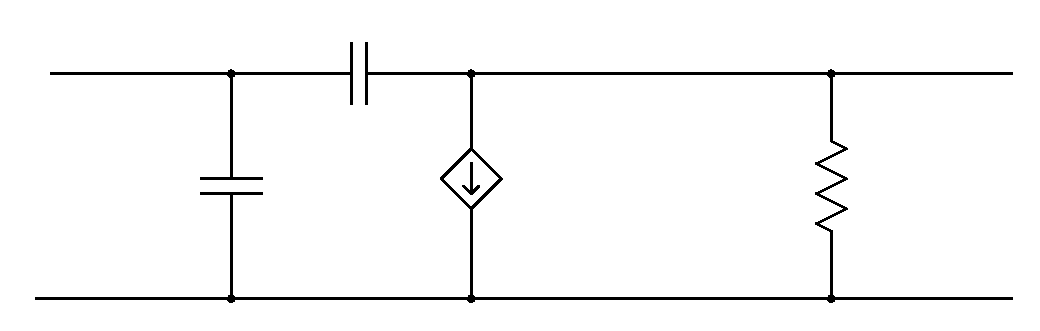
\includegraphics[scale=0.90]{MOSFETsmallSignalHighFrequencyModel}
\caption{بلند تعددی باریک اشاراتی ماسفیٹ پائے ماڈل}
\label{شکل_باریک_اشاراتی_بلند_تعددی_ماسفیٹ_ماڈل}
\end{figure}
کم \عددی{v_{DS}} کی صورت میں غیر افزائندہ ماسفیٹ کے گیٹ کے  نیچے \اصطلاح {الٹا خطہ} سورس سے ڈرین تک تقریباً یکساں شکل کا ہوتا ہے۔گیٹ اور \اصطلاح {الٹا خطہ} مل کر کپیسٹر \عددی{\tfrac{\epsilon W L}{d}} کو جنم دیتے ہیں۔اس کپیسٹر کا آدھا حصہ \عددی{C_{gs}} اور آدھا \عددی{C_{gd}} ہے یعنی
\begin{align}
C_{gs} \approx C_{gd} \approx \left(\frac{1}{2} \right)\frac{\epsilon W L}{d}
\end{align} 
جہاں \عددی{W}  گیٹ کی چوڑائی، \عددی{L} گیٹ کی لمبائی، \عددی{d} گیٹ اور سلیکان کے درمیان فاصلہ ہے۔\عددی{\epsilon = \epsilon_r \epsilon_0} ہے جہاں \عددی{\epsilon_r=3.9} جبکہ \عددی{\epsilon_0=\SI{8.85e-12}{\farad \per \meter}} ہے۔

افزائندہ ماسفیٹ کے ڈرین جانب راہ دبوچا گیا ہوتا ہے۔یوں گیٹ کے نیچے پیدا کردہ راہ ہر جگہ یکساں نہیں  ہوتا۔اس صورت میں \عددی{C_{gd} \approx 0} جبکہ \عددی{C_{gs} \approx \tfrac{2 \epsilon W L}{3 d}} ہوتا ہے۔
\begin{gather}
\begin{aligned}
C_{gd}& \approx 0\\
C_{gs}& \approx \left(\frac{2}{3}\right) \frac{\epsilon WL}{d}
\end{aligned}
\end{gather} 

ان کے علاوہ گیٹ کا کچھ حصہ سورس کو اور کچھ حصہ ڈرین کو ڈھانپتا ہے  جس سے گیٹ اور سورس کے مابین غیر مطلوب کپیسٹر \عددی{C_{gsp}} اور اسی طرح گیٹ اور ڈرین کے مابین غیر مطلوب کپیسٹر \عددی{C_{gsp}} پیدا ہوتا ہے۔ڈرین اور سلیکان پتری کا مابین \عددی{pn} جوڑ پایا جاتا ہے جس کے کپیسٹر کو \عددی{C_{db}} سے ظاہر کیا جاتا ہے۔

ماسفیٹ کے ماڈل میں \عددی{C_{gs}} گیٹ اور سورس کے درمیان دونوں اقسام کے کپیسٹروں کے مجموعے کو کہتے ہیں۔اسی طرح \عددی{C_{gd}} بھی دونوں اقسام کے کپیسٹروں کے مجموعے کو ظاہر کرتا ہے۔شکل \حوالہ{شکل_ماسفیٹ_ماڈل_اجزاء} میں ان تمام قسم کے کپیسٹروں کو دکھایا گیا ہے۔ساتھ ہی ساتھ مزاحمت \عددی{r_s} اور \عددی{r_d} بھی دکھائے گئے ہیں۔بیرونی سورس سرے اور اندرونی سورس کے درمیان \عددی{r_s} مزاحمت پایا جاتا ہے۔اسی طرح بیرونی ڈرین سرے اور اندرونی ڈرین کے درمیان \عددی{r_d} پایا جاتا ہے۔اس کتاب میں \عددی{C_{db}}، \عددی{r_s} اور \عددی{r_d} کو  استعمال نہیں کیا جائے گا۔
\begin{figure}
\centering
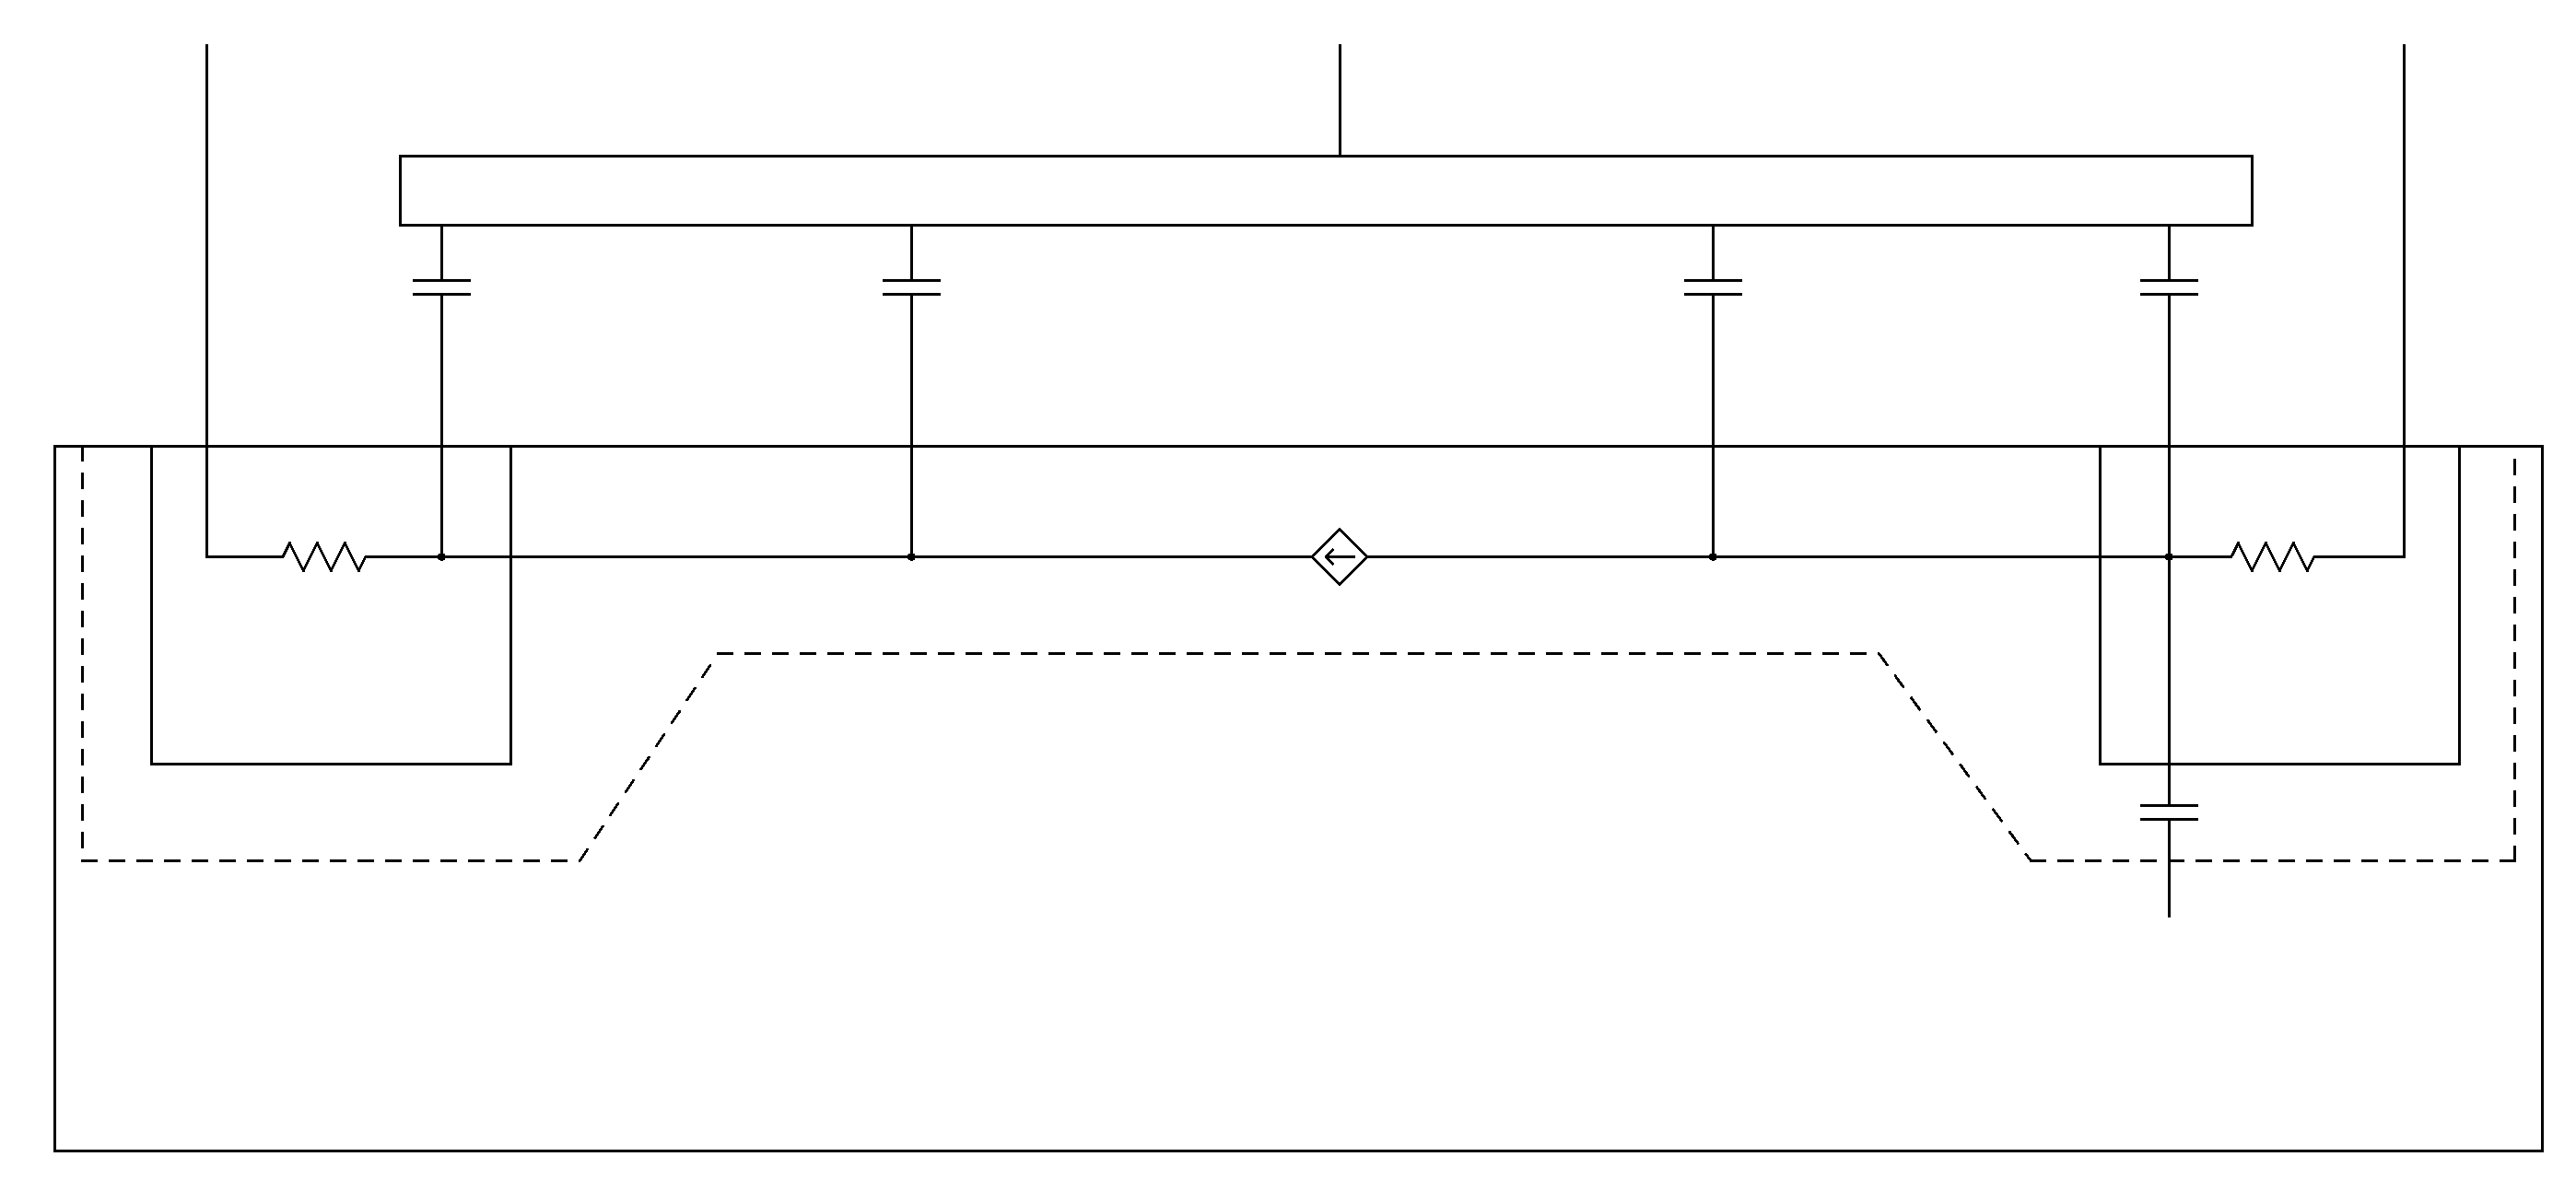
\includegraphics[scale=0.90]{mosfetCapacitors}
\caption{ماسفیٹ ماڈل کے اجزاء}
\label{شکل_ماسفیٹ_ماڈل_اجزاء}
\end{figure}

دو جوڑ ٹرانزسٹر کے پائے ماڈلوں کی طرح ماسفیٹ کے باریک اشاراتی پائے ماڈل \تحریر{nMOSFET} اور \تحریر{pMOSFET} دونوں کے لئے یکساں قابل استعمال ہیں۔
%=====================
\جزوحصہ{باریک اشاراتی ماسفیٹ ٹی ماڈل}
شکل \حوالہ{شکل_ماسفیٹ_ٹی_ماڈل} الف میں \عددیء{r_o} کو نظر انداز کرتے ہوئے ماسفیٹ کا \اصطلاح {ٹی ماڈل}\فرہنگ{ٹی ماڈل}\فرہنگ{ماڈل!ٹی}\حاشیہب{T model}\فرہنگ{T model} دکھایا گیا ہے۔اس ماڈل میں گیٹ اور سورس کے مابین مزاحمت نسب ہے جس کی قیمت \عددیء{\tfrac{1}{g_m}} ہے۔اس ماسفیٹ ماڈل کو پائے ماڈل سے یوں حاصل کیا جا سکتا ہے۔پائے ماڈل میں
\begin{gather} 
\begin{aligned}\label{مساوات_ماسفیٹ_ٹی_ماڈل_کے_برقی_رو}
i_g&=0\\
i_d&=i_s=i_{ds}=g_m v_{gs}
\end{aligned}
\end{gather}
پائے جاتے ہیں جہاں \عددیء{i_d} اور \عددیء{i_s} ڈرین اور سورس کے برقی رو ہیں۔داخلی مزاحمت لامحدود ہے۔آئیں اب ٹی ماڈل پر نظر ڈالیں۔ٹی ماڈل میں \عددیء{i_d=g_m v_{gs}} ہے۔گیٹ اور سورس کے مابین مزاحمت نسب ہے جس پر برقی دباو \عددیء{v_{gs}} ہے۔یوں اُوہم کے قانون سے اس مزاحمت میں برقی رو کی مقدار
\begin{align*}
\frac{\textrm{دباو برقی}}{\textrm{رو برقی}}=\frac{v_{gs}}{\frac{1}{g_m}}=g_m v_{gs}
\end{align*} 
ہو گی۔یہی برقی رو سورس پر ہو گی۔گیٹ \عددیء{G} کے جوڑ پر \عددیء{D} کی جانب سے \عددیء{g_m v_{gs}} برقی رو آتی ہے۔اس جوڑ سے اتنی ہی برقی رو مزاحمت سے گزرتے ہوئے \عددیء{S} رواں ہے۔یوں کرچاف کے قانون برائے برقی رو کی مدد سے گیٹ  پر برقی رو \عددیء{i_g=0} حاصل ہوتی ہے۔داخلی مزاحمت \عددیء{\tfrac{v_{gs}}{i_g}} کی قیمت \عددیء{i_g=0} کی بنا پر لامحدود حاصل ہوتی ہے۔ہم دیکھتے ہیں کہ ٹی ماڈل سے بھی بالکل وہی جوابات حاصل ہوتے ہیں جو پائے ماڈل سے حاصل ہوتے ہیں لہٰذا ماسفیٹ کے ادوار حل کرتے وقت ٹی ماڈل کو بھی استعمال کیا جا سکتا ہے۔ٹی ماڈل میں \عددیء{r_o} کی شمولیت شکل \حوالہ{شکل_ماسفیٹ_ٹی_ماڈل} ب میں دکھایا گیا ہے۔ 

%
\begin{figure}
\centering
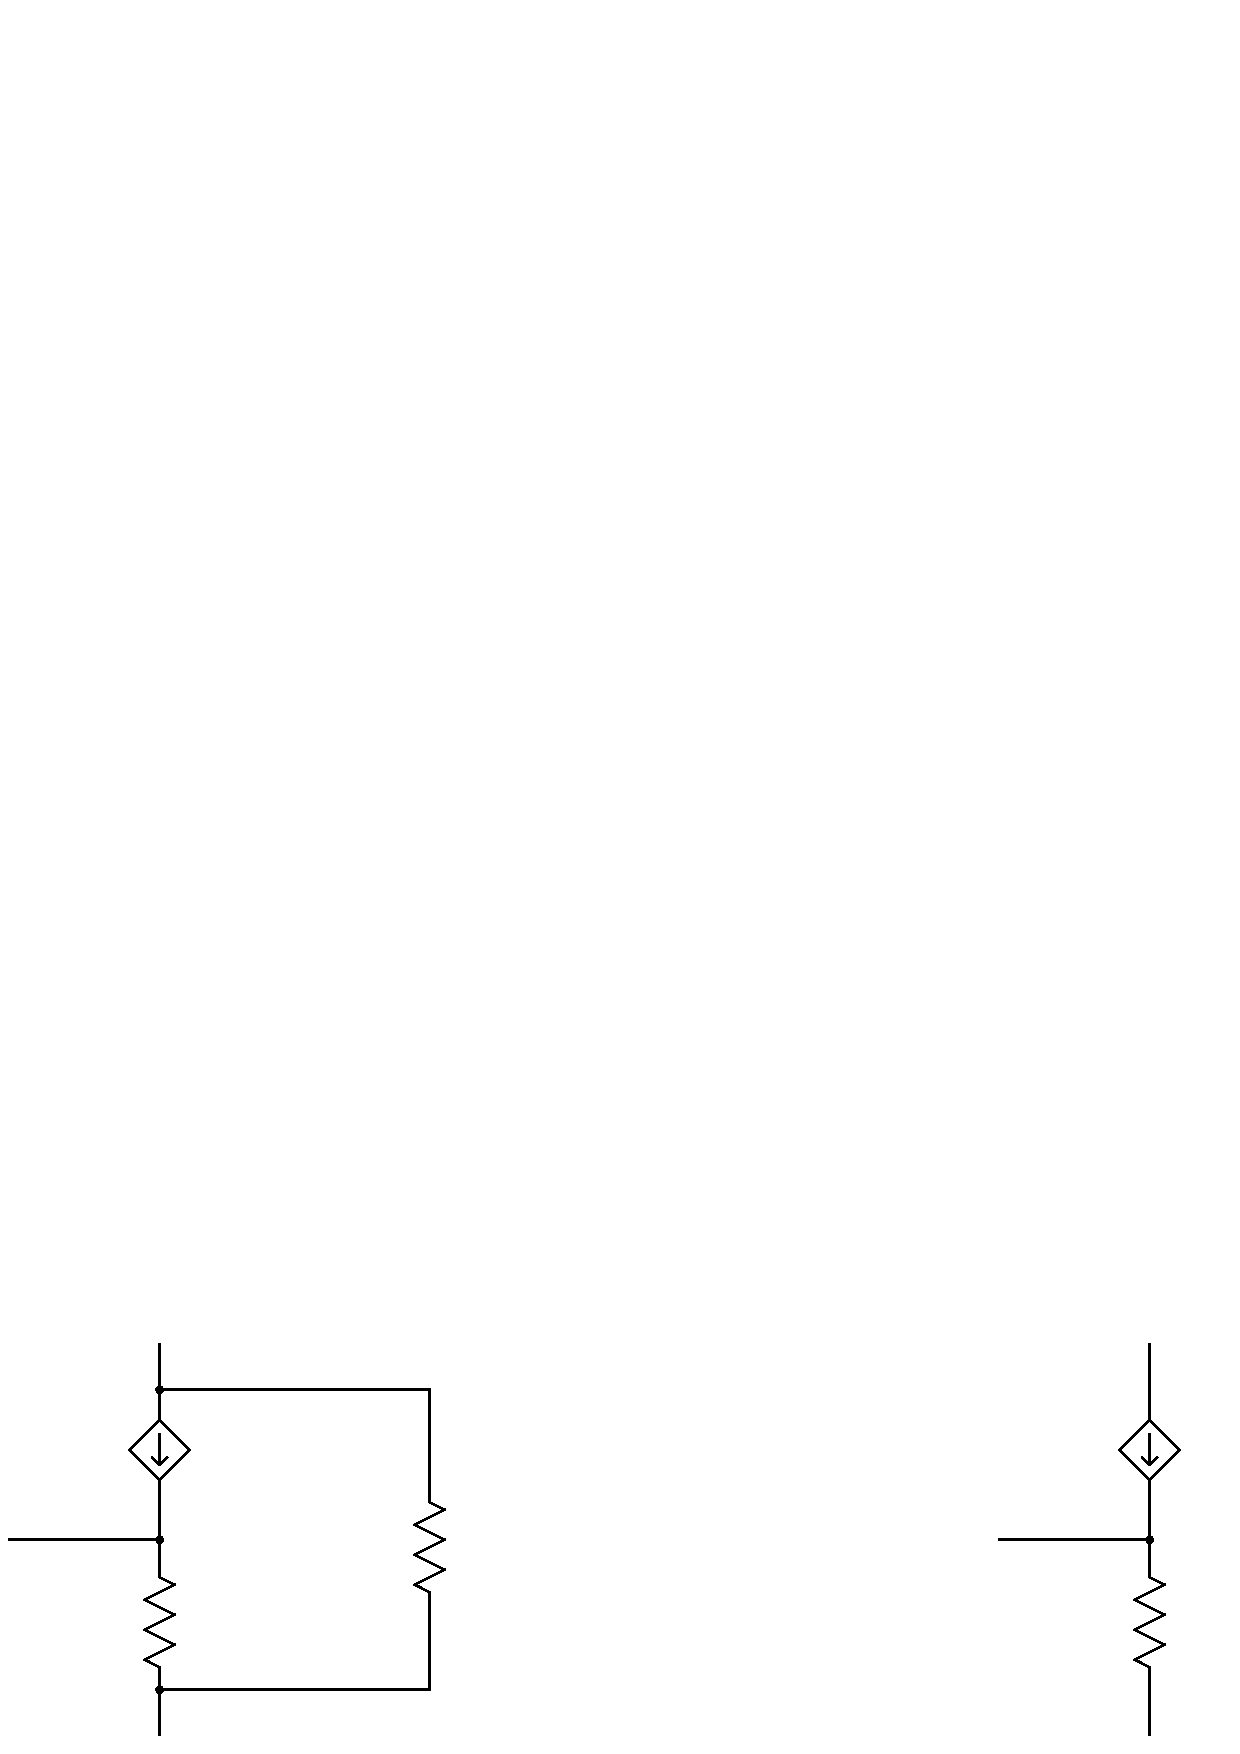
\includegraphics[scale=0.90]{mosfetTmodel}
\caption{باریک اشاراتی ماسفیٹ ٹی ماڈل}
\label{شکل_ماسفیٹ_ٹی_ماڈل}
\end{figure}

دو جوڑ ٹرانزسٹر کے ٹی ماڈل کی طرح  شکل \حوالہ{شکل_ماسفیٹ_ٹی_ماڈل} میں دکھائے گئے ماسفیٹ کے ٹی ماڈل \تحریر{nMOSFET} اور \تحریر{pMOSFET} دونوں کے لئے قابل استعمال ہیں۔
 

\جزوحصہ{یک سمتی اور بدلتے متغیرات کی علیحدگی}
مندرجہ بالا تذکرہ سے ہم دیکھتے ہیں کہ برقی دباو اور برقی رو کے دو حصے (یعنی یک سمتی حصہ اور بدلتا حصہ) ہوتے ہے۔ماسفیٹ کے ادوار حل کرتے وقت ان دو حصوں کو علیحدہ علیحدہ حل کیا جاتا ہے۔پہلے بدلتے متغیرات کی قیمتیں صفر کرتے ہوئے یک سمتی حصہ حل کر کے نقطہ مائل حاصل کیا جاتا ہے اور پھر بدلتے حصے کو ماڈل کی مدد سے حل کیا جاتا ہے۔
%=========
\ابتدا{مثال}
مساوات \حوالہ{مساوات_میدانی_رو_کے_حصے} میں \عددی{\tfrac{k_n v_{gs}^2}{2}} نا پسندیدہ حصہ ہے۔اگر داخلی اشارہ \عددی{v_{gs}=V_p \cos \omega t} ہو تب نا پسندیدہ جزو میں \عددی{\cos ^2 \omega t=\tfrac{1+\cos (2 \omega t)}{2}} استعمال کرتے ہوئے  \عددی{\tfrac{k_n V_p^2}{4} \left[1+\cos (2 \omega t) \right]} لکھا جا سکتا ہے جو داخلی اشارے کے دگنی تعدد کا جزو  ہے۔یہی اصل اشارے کی شکل \اصطلاح {بگاڑتا} ہے۔خارجی اشارے میں دگنی تعدد اور اصل تعدد کے اجزاء کے حیطوں کی نسبت حاصل کریں۔اگر \عددی{V_t=\SI{1.4}{\volt}} اور \عددی{V_{GS}=\SI{4}{\volt}} ہوں تب داخلی اشارے کی چوٹی کی وہ حد حاصل کریں جس پر حاصل کردہ نسبت \عددی{\SI{1}{\percent}} ہو۔

حل:دگنی تعدد کا حصہ \عددی{\tfrac{k_n V_p^2}{4} \cos (2 \omega t)} ہے۔یوں
\begin{align*}
\frac{\textrm{بگڑا جزو}}{\textrm{اصل جزو}}=\frac{V_p}{4 \left(V_{GS}-V_t \right)}
\end{align*}
حاصل ہوتا ہے۔اس طرح
\begin{align*}
\frac{V_p \times 100}{4 \left(4-1.4\right)}=1
\end{align*}
سے  \عددی{V_p \le \SI{104}{\milli \volt}} حاصل ہوتا ہے۔
\انتہا{مثال}
%===================

\ابتدا{مثال}
ایک دور جسے شکل \حوالہ{شکل_ماسفیٹ_کے_یک_سمتی_ادوار_ب} ب میں دکھایا گیا ہے کا تجزیہ کرتے ہوئے مندرجہ ذیل معلومات حاصل کئے جاتے ہیں۔
\begin{align*}
V_{DD}&=\SI{12}{\volt}\\
R_D&=\SI{6.8}{\kilo \ohm}\\
R_S&=\SI{5.6}{\kilo \ohm}\\
R_{G1}&=R_{G2}=\SI{10}{\mega \ohm}
\end{align*}
ہیں۔مزید اس کے گیٹ پر \عددی{V_G=\SI{6}{\volt}} جبکہ سورس پر \عددی{V_S=\SI{0.81}{\volt}} ناپے جاتے ہیں۔ساتھ ہی ساتھ باریک اشاراتی برقی دباو کی افزائش \عددی{A_v=\SI{-6.8}{\volt \per \volt}} ناپی جاتی ہے جہاں خارجی اشارے کو ڈرین سے لیا گیا۔استعمال کئے گئے ماسفیٹ کی \عددی{k_n} اور \عددی{V_t} حاصل کریں۔

حل:اُوہم کے قانون سے
\begin{align*}
I_{DS}=\frac{V_S}{R_S}=\frac{0.81}{5600}=\SI{1.4464}{\milli \ampere}
\end{align*}
حاصل ہوتا ہے۔ساتھ ہی ساتھ
\begin{align*}
V_{GS}=V_G-V_S=6-0.81=\SI{5.19}{\volt}
\end{align*}
ہے۔مساوات \حوالہ{مساوات_ماسفیٹ_افزائش_کی_سادہ_مساوات} کی مدد سے \عددی{g_m=\SI{1}{\milli \ampere \per volt}} حاصل کرتے ہوئے مساوات \حوالہ{مساوات_میدانی_موصلیت_نما_بطور_افزائش} میں پر کرتے ملتا ہے۔
\begin{align*}
10^{-3}=k_n \left(5.19-V_t \right)
\end{align*}
تصور کرتے ہیں کہ ماسفیٹ افزائندہ خطے میں ہے یوں افزائندہ ماسفیٹ کی مساوات سے
\begin{align*}
1.4464 \times 10^{-3}=\frac{k_n}{2} \left(5.19-V_t \right)^2
\end{align*}
حاصل ہوتا ہے۔مندرجہ بالا دو نتائج ملا کر
\begin{align*}
1.4464 \times 10^{-3}=\frac{k_n}{2} \left( \frac{10^{-3}}{k_n}\right)^2
\end{align*}
لکھا جا سکتا ہے جس سے \عددی{k_n=\SI{0.345}{\milli \ampere \per \volt \squared}} حاصل ہوتا ہے۔اس قیمت کو استعمال کرتے ہوئے \عددی{V_t=\SI{2.29}{\volt}} حاصل ہوتا ہے۔

شکل کو دیکھتے ہوئے
\begin{align*}
V_D=V_DD-I_{DS} R_D=15-1.4464 \times 10^{-3} \times 6800=\SI{5.16}{\volt}
\end{align*}
لکھا جا سکتا ہے۔یوں
\begin{align*}
V_{GD}=V_G-V_D=6-5.16=\SI{0.835}{\volt}
\end{align*}
حاصل ہوتا ہے جو \عددی{V_t} سے کم ہے لہٰذا ماسفیٹ افزائندہ خطے میں ہی ہے۔
\انتہا{مثال}
%=============
\ابتدا{مثال}
شکل \حوالہ{شکل_ماسفیٹ_ایمپلیفائر_مثال} میں ماسفیٹ ایمپلیفائر دکھایا گیا ہے۔داخلی اور خارجی جانب لامحدود جفتی کپیسٹر استعمال کئے گئے ہیں۔داخلی مزاحمت، خارجی مزاحمت اور افزائش \عددی{A_v=\tfrac{v_L}{v_s}} حاصل کریں۔

\begin{figure}
\centering
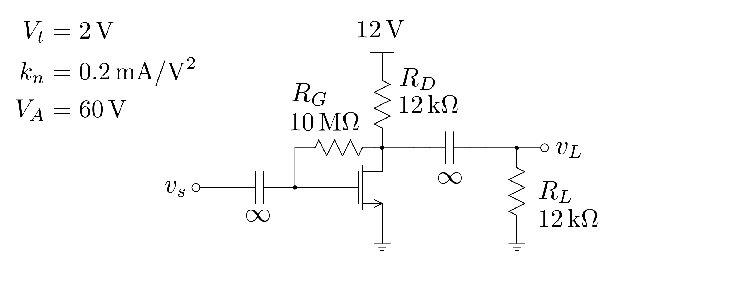
\includegraphics[scale=0.90]{mosfetAmplifierGateToSourceResistor}
\caption{ماسفیٹ ایمپلیفائر}
\label{شکل_ماسفیٹ_ایمپلیفائر_مثال}
\end{figure}

حل:چونکہ گیٹ پر برقی رو صفر ہے لہٰذا \عددی{R_G} پر صفر وولٹ کا گھٹاو ہو گا۔اس طرح \عددی{V_G=V_D} ہوں گے، یعنی \عددی{V_{GS} = V_{DS}} ہو گا، لہٰذا \عددی{V_{GD}=\SI{0}{\volt}} ہو گا۔یوں \عددی{V_{GD} < V_t} ہے جس سے ثابت ہوتا ہے کہ ماسفیٹ افزائندہ خطے میں ہے۔یوں
\begin{align*}
I_{DS}&=\frac{0.2 \times 10^{-3}}{2} \left(V_{GS}-2 \right)^2\\
&=\frac{0.2 \times 10^{-3}}{2} \left(V_{DS}-2 \right)^2
\end{align*}
لکھا جا سکتا ہے۔اُوہم کے قانون سے
\begin{align*}
I_{DS}=\frac{12-V_{DS}}{R_D}=\frac{12-V_{DS}}{12000}
\end{align*}
حاصل ہوتا ہے۔ان دو مساوات کو ملا کر حل کرنے سے
\begin{align*}
V_{DS}=\SI{4.5}{\volt},\hspace{3mm} I_{DS}=\SI{0.625}{\milli \ampere}
\end{align*}
حاصل ہوتا ہے۔دو درجی مساوات کے دوسرے جواب کو رد کیا جاتا ہے۔

\عددی{g_m} کی قیمت
\begin{align*}
g_m&=k_n \left(V_{GS}-V_t \right)\\
&=0.2 \times 10^{-3} \left(4.5-2 \right)\\
&=\SI[per=frac,fraction=nice]{0.5}{\milli \ampere \per \volt}
\end{align*}
اور  خارجی مزاحمت \عددی{r_o} کی قیمت
\begin{align*}
r_o=\frac{V_A}{I_{DS}}=\frac{60}{0.625 \times 10^{-3}}=\SI{96}{\kilo \ohm}
\end{align*}
حاصل ہوتے ہیں۔شکل \حوالہ{شکل_ماسفیٹ_ایمپلیفائر_مساوی_باریک_اشاراتی_دور_مثال} میں ان قیمتوں کو استعمال کرتے ہوئے مساوی پست تعددی باریک اشاراتی  دور دکھایا گیا ہے۔
\begin{figure}
\centering
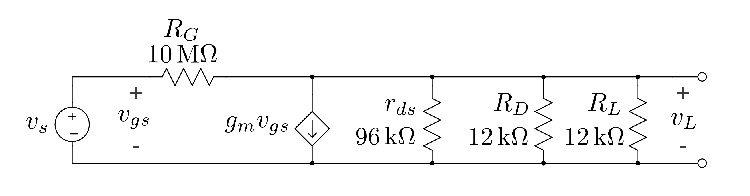
\includegraphics[scale=0.90]{mosfetAmplifierGateToSourceResistorEquivalent}
\caption{ماسفیٹ ایمپلیفائر کا مساوی باریک اشاراتی دور}
\label{شکل_ماسفیٹ_ایمپلیفائر_مساوی_باریک_اشاراتی_دور_مثال}
\end{figure}
\عددی{R_G} سے گزرتے برقی رو کو نظر انداز کرتے ہوئے
\begin{align*}
v_L& \approx -g_m v_{gs} \left(r_o \mathbin{\|} R_D \mathbin{\|} R_L \right)\\
&=-2.823 v_{gs}
\end{align*}
حاصل ہوتا ہے۔چونکہ \عددی{v_{gs}} اور \عددی{v_s} برابر ہیں لہٰذا 
\begin{align*}
A_v=\frac{v_L}{v_s}=\SI[per=frac,fraction=nice]{-2.823}{\volt \per \volt}
\end{align*}
حاصل ہوتا ہے۔چونکہ \عددی{R_G} میں برقی رو

\begin{align*}
i_s &=\frac{v_s-v_L}{R_G}\\
&=\frac{v_s}{R_G} \left(1-\frac{v_L}{v_s} \right)\\
&=\frac{v_s}{R_G} \left[1-(-2.823) \right]\\
&=3.823 \frac{v_s}{R_G}
\end{align*}
کے برابر ہے لہٰذا داخلی مزاحمت
\begin{align*}
R_i=\frac{v_s}{i_s}=\frac{R_G}{3.823}=\SI{2.6}{\mega \ohm}
\end{align*}
حاصل ہوتا ہے۔
\انتہا{مثال}
%===================
\ابتدا{مثال}\شناخت{مثال_ماسفیٹ_مشترک_مخارج_بمع_مزاحمت}
شکل \حوالہ{شکل_ماسفیٹ_مخارج_مزاحمت_کے_ساتھ} میں \عددی{V_t=\SI{0.8}{\volt}} اور \عددی{k_n=\SI{1.2}{\milli \ampere \per \volt \squared}} ہیں۔\عددی{r_o} کو نظر انداز کرتے ہوئے \عددی{A_v=\tfrac{v_L}{v_i}} حاصل کریں۔کپیسٹر کی قیمت لامحدود تصور کریں۔
\begin{figure}
\centering
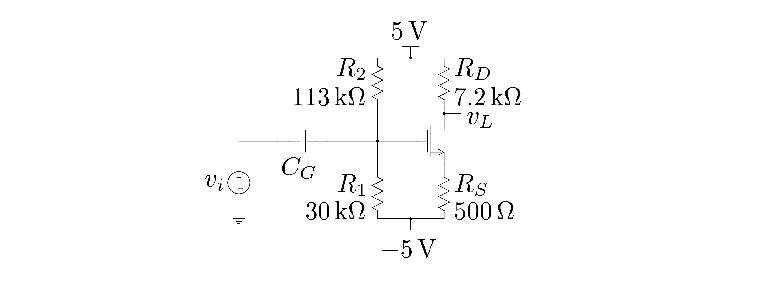
\includegraphics[scale=0.90]{mosfetCommonSourceAmplifierWithSourceResistor}
\caption{مشترک ایمٹر بمع ایمٹر مزاحمت}
\label{شکل_ماسفیٹ_مخارج_مزاحمت_کے_ساتھ}
\end{figure}

حل:یک سمتی تجزیہ سے \عددیء{I_{DS}=\SI{0.6}{\milli \ampere}}، \عددی{V_{GS}=\SI{1.8}{\volt}} اور \عددی{V_{DS}=\SI{5.38}{\volt}} حاصل ہوتے ہیں۔یوں ماسفیٹ افزائندہ خطے میں ہے۔انہیں استعمال کرتے ہوئے
\begin{align*}
g_m=\sqrt{2 k_n I_{DS}}=\sqrt{2 \times 1.2 \times 10^{-3} \times 0.6 \times 10^{-3}}=\SI{1.2}{\milli \siemens}
\end{align*}
حاصل ہوتا ہے۔ایمپلیفائر کا باریک اشاراتی مساوی دور شکل \حوالہ{شکل_ماسفیٹ_مخارج_مزاحمت_کے_ساتھ_مساوی} میں دکھایا گیا ہے جس سے
\begin{align*}
v_L&=-g_m v_{gs} R_D=-8.64 v_{gs}\\
v_g&=v_i\\
v_s&=g_m v_{gs} R_S=0.6 v_{gs}
\end{align*}
حاصل ہوتے ہیں۔چونکہ \عددی{v_{gs}=v_g - v_s } ہے لہٰذا
\begin{align*}
v_{gs}=v_i-0.6v_{gs}
\end{align*}
لکھا جا سکتا ہے جس سے
\begin{align*}
v_{gs}=\frac{v_i}{1.6}=0.625 v_{i}
\end{align*}
حاصل ہوتا ہے۔اس قیمت کو \عددی{v_L} کی مساوات میں پُر کرتے ملتا ہے 
\begin{align*}
v_L=-8.64 \times 0.625 \times v_i=-5.4 v_i
\end{align*}
یعنی
\begin{align*}
A_v=\frac{v_L}{v_i}=\SI{-5.4}{\volt \per \volt}
\end{align*}
%
\begin{figure}
\centering
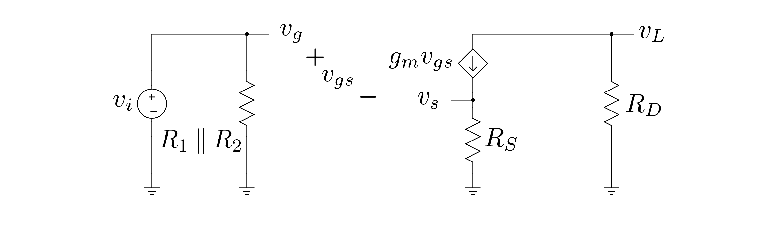
\includegraphics[scale=0.90]{mosfetCommonSourceAmplifierWithSourceResistorEquivalent}
\caption{مشترک ایمٹر بمع ایمٹر مزاحمت کا باریک اشاراتی مساوی دور}
\label{شکل_ماسفیٹ_مخارج_مزاحمت_کے_ساتھ_مساوی}
\end{figure}
\انتہا{مثال}
%===========================
\ابتدا{مثال}
مثال \حوالہ{مثال_ماسفیٹ_مشترک_مخارج_بمع_مزاحمت} میں \عددی{R_S} کے متوازی لامحدود قیمت کا کپیسٹر نسب کرتے ہوئے \عددی{A_v} دوبارہ حاصل کریں۔

حل:کپیسٹر نسب کرنے سے نقطہ کارکردگی پر کوئی اثر نہیں پڑتا لہٰذا \عددی{g_m=\SI{1.2}{\milli  \siemens}} ہی رہے گا۔باریک اشاراتی مساوی دور شکل \حوالہ{شکل_ماسفیٹ_مخارج_مزاحمت_کے_متوازی_کپیسٹر_مساوی} میں دکھایا گیا ہے جس سے
\begin{align*}
v_L&=-g_m v_{gs} R_D=-8.64 v_{gs}\\
v_g&=v_i\\
v_s&=0
\end{align*}
یعنی
\begin{align*}
v_{gs}&=v_i\\
v_L&=-8.64 v_i
\end{align*}
اور 
\begin{align*}
A_v=\SI{-8.64}{\volt \per \volt}
\end{align*}
حاصل ہوتے ہیں۔
%
\begin{figure}
\centering
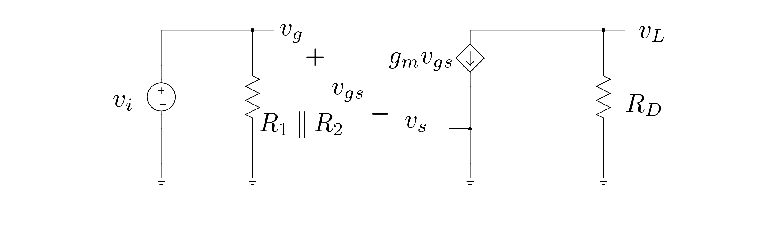
\includegraphics[scale=0.90]{mosfetCommonSourceAmplifierWithSourceResistorBypassedEquivalent}
\caption{}
\label{شکل_ماسفیٹ_مخارج_مزاحمت_کے_متوازی_کپیسٹر_مساوی}
\end{figure}
\انتہا{مثال}
%===============
ان دو مثالوں سے آپ دیکھتے ہیں کہ \عددی{R_S} کی شمولیت سے \عددی{A_v} گھٹتا ہے لیکن چونکہ \عددی{R_S} کے استعمال سے نقطہ کارکردگی مستحکم ہوتا ہے لہٰذا \عددی{R_S} کا استعمال کیا جاتا ہے۔\عددی{R_S} کے متوازی لامحدود کپیسٹر نسب کرنے سے \عددی{A_v} پر \عددی{R_S} کے بُرے اثر کو ختم کیا جاتا ہے۔
%===================
\ابتدا{مثال}
شکل \حوالہ{شکل_ماسفیٹ_افزائش_بطور_کسر_مزاحمت_الف} الف کے ایمپلیفائر کو ٹی ماڈل سے حل کریں۔ 
\begin{figure}
\centering
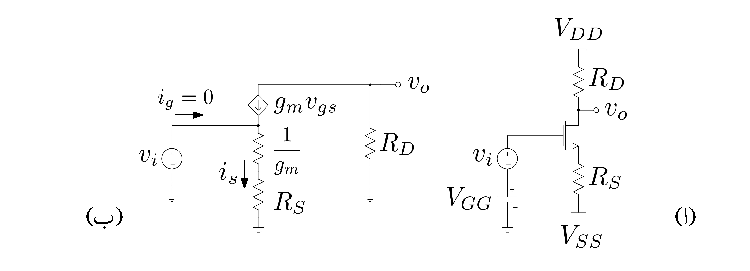
\includegraphics[scale=0.90]{gainAsResistorRatioA}
\caption{}
\label{شکل_ماسفیٹ_افزائش_بطور_کسر_مزاحمت_الف}
\end{figure}

حل:شکل  ب میں ٹی ماڈل استعمال کرتے ہوئے اس کا باریک اشاراتی مساوی دور دکھایا گیا ہے۔ٹی ماڈل استعمال کرتے وقت اس حقیقت کو بروئے کار لائیں کہ گیٹ پر برقی رو صفر رہتی ہے۔شکل میں \عددیء{i_g=0} لکھ کر اس حقیقت کی یاد دہانی کرائی گئی ہے۔داخلی جانب کرچاف کے قانون برائے برقی دباو کی مدد سے ہم لکھ سکتے ہیں۔
\begin{align*}
i_s=\frac{v_i}{\frac{1}{g_m}+R_S}
\end{align*}
چونکہ \عددیء{i_g=0} ہے لہٰذا یہی برقی رو \عددیء{R_D} سے بھی گزرے گی۔اس طرح
\begin{align*}
v_o=-\left(\frac{v_i}{\frac{1}{g_m}+R_S} \right) R_D
\end{align*}
ہو گا۔جس سے
\begin{align}
A_v=\frac{v_o}{v_i}=-\left(\frac{R_D}{\frac{1}{g_m}+R_S} \right) 
\end{align}
حاصل ہوتا ہے۔اس مساوات کو یوں بہتر طرز پر لکھا جا سکتا ہے
\begin{align}\label{مساوات_ماسفیٹ_افزائش_بطور_مزاحت_کی_شرح}
A_v=-\frac{\sum R_{\textrm{ڈرین}}}{\sum R_{\textrm{سورس}}}
\end{align}
صفحہ \حوالہصفحہ{مساوات_ٹرانزسٹر_ایمپلیفائر_کی_افزائش_کلکٹر _مخارج_مزاحمتوں_کی_شرح} پر مساوات \حوالہ{مساوات_ٹرانزسٹر_ایمپلیفائر_کی_افزائش_کلکٹر _مخارج_مزاحمتوں_کی_شرح} میں \عددیء{\alpha=1} لیتے ہوئے مساوات \حوالہ{مساوات_ماسفیٹ_افزائش_بطور_مزاحت_کی_شرح} ہی حاصل ہوتا ہے۔دو جوڑ ٹرانزسٹر کی صورت میں \عددیء{\tfrac{1}{g_m}} کو \عددیء{r_e} لکھا گیا جبکہ یہاں  ہم اس کو \عددیء{\tfrac{1}{g_m}} ہی لکھیں گے۔
\انتہا{مثال}
%==================
\حصہ{سیماس نفی کار}\شناخت{حصہ_ماسفیٹ_نفی_کار}
\اصطلاح {عددی ادوار}\فرہنگ{عددی ادوار}\حاشیہب{digital circuits}\فرہنگ{digital circuits} میں \اصطلاح {نفی کار}\فرہنگ{نفی کار}\حاشیہب{NOT gate}\فرہنگ{NOT gate} کلیدی کردار ادا کرتا ہے۔جیسا کہ پہلے بھی ذکر کیا گیا، سیماس ٹیکنالوجی کی بہتر خصوصیات کی بنا پر مخلوط ادوار زیادہ تر انہیں کو استعمال کرتے ہوئے بنائے جاتے ہیں۔ 
\begin{figure}
\centering
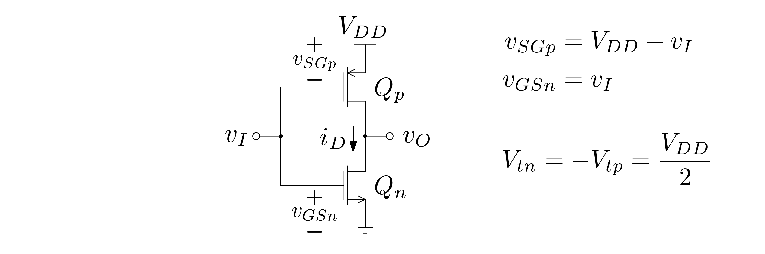
\includegraphics[scale=0.90]{NOTgateCMOS}
\caption{نفی کار}
\label{شکل_ماسفیٹ_نفی_کار_الف}
\end{figure}

شکل \حوالہ{شکل_ماسفیٹ_نفی_کار_الف}  الف میں ایک عدد \تحریر{pMOSFET} اور ایک عدد \تحریر{nMOSFET} استعمال کرتے ہوئے  نفی کار بنایا گیا ہے۔عددی اشارات صرف دو ہی قیمتیں \عددیء{\SI{0}{\volt}} یعنی پست صورت  یا \عددیء{\SI{5}{\volt}} یعنی بلند صورت اختیار کر سکتے ہیں۔آئیں \عددیء{v_I} کو ان قیمتوں پر رکھتے ہوئے خارجی اشارہ \عددیء{v_O} حاصل کریں۔شکل کو دیکھتے ہوئے
\begin{gather}
\begin{aligned}\label{مساوات_ماسفیٹ_ناٹ_گیٹ_الف}
v_{SGp}&=V_{DD}-v_I\\
v_{GSn}&=v_I
\end{aligned}
\end{gather}
لکھا جا سکتا ہے۔مزید تصور کریں کہ 
\begin{align}
V_{tn}=-V_{tp}=V_t
\end{align}
کے برابر ہے۔

داخلی اشارہ \عددیء{v_I=\SI{0}{\volt}} کی صورت میں مساوات \حوالہ{مساوات_ماسفیٹ_ناٹ_گیٹ_الف} سے \عددیء{v_{GSn}=\SI{0}{\volt}} حاصل ہوتا ہے۔چونکہ \عددیء{V_{tn}} مثبت مقدار ہے  لہٰذا  \عددیء{v_{GSn} < V_{tn}} ہے۔اس طرح  \عددیء{Q_n} منقطع ہو گا اور اس کی برقی رو صفر ہو گی۔اس کے برعکس \عددیء{Q_p} کے لئے  مساوات \حوالہ{مساوات_ماسفیٹ_ناٹ_گیٹ_الف} کے مطابق \عددیء{v_{SGp}=V_{DD}} حاصل ہوتا ہے۔یوں \عددیء{v_{SGp} > -V_{tp}} ہے لہٰذا \عددیء{Q_p} چالو ہو گا۔شکل \حوالہ{شکل_ماسفیٹ_نفی_کار_داخلی_پست_خارجی_بلند} میں منقطع \عددیء{Q_n} کے خط پر چالو \عددیء{Q_p} کے خط کو بطور خطِ بوجھ دکھایا گیا ہے۔\عددیء{Q_p} کے خط کا عمودی محور میں عکس لینے کے بعد اس عکس کو افقی محور پر دائیں جانب \عددیء{V_{DD}} اکایاں منتقل کرنے سے خطِ بوجھ\حاشیہد{صفحہ \حوالہصفحہ{حصہ_ٹرانزسٹر_نفی_کار} پر حصہ \حوالہ{حصہ_ٹرانزسٹر_نفی_کار} کے شروع میں  ٹرانزسٹر خطِ بوجھ کھینچنا دکھایا گیا۔اس طریقے پر ایک مرتبہ دوبارہ نظر ڈالیں۔} حاصل ہوتا ہے ۔\عددیء{Q_n} کے خط کو افقی محور سے قدر اوپر کر کے دکھایا گیا ہے تا کہ یہ محور سے علیحدہ نظر آئے۔ان دو خطوط سے حاصل نقطہ کارکردگی کے مطابق \عددیء{v_{DSQ} \approx V_{DD}} کے برابر ہے۔اس طرح \عددیء{v_I=0} کی صورت میں \عددیء{v_O=V_{DD}} حاصل ہوتا ہے۔

یہی جواب خطوط کھینچے بغیر  یوں حاصل کیا جا سکتا ہے۔منقطع \عددیء{Q_n} کو کھلے دور جبکہ چالو \عددیء{Q_p} کو بطور مزاحمت تصور کریں۔ایسا کرنے سے شکل \حوالہ{شکل_ماسفیٹ_نفی_کار_داخلی_پست_خارجی_بلند} میں دکھایا دور حاصل ہوتا ہے جس کو دیکھ کر  \عددیء{v_O=V_{DD}} لکھا جا سکتا ہے۔ 

\begin{figure}
\centering
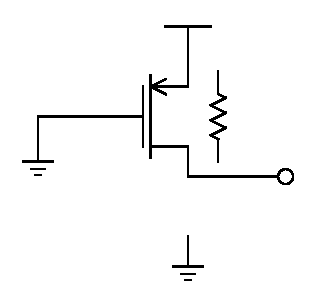
\includegraphics[scale=0.90]{NOTgateLowInput}
\caption{داخلی اشارہ پست ہونے کی صورت میں خارجی اشارہ بلند حاصل ہوتا ہے۔}
\label{شکل_ماسفیٹ_نفی_کار_داخلی_پست_خارجی_بلند}
\end{figure}

داخلی اشارہ \عددیء{v_I=V_{DD}} کی صورت میں مساوات \حوالہ{مساوات_ماسفیٹ_ناٹ_گیٹ_الف} سے \عددیء{v_{GSn}=V_{DD}} حاصل ہوتا ہے لہٰذا  \عددیء{v_{GSn} > V_{tn}} ہے۔اس طرح  \عددیء{Q_n} چالو ہو گا۔اس کے برعکس \عددیء{Q_p} کے لئے  مساوات \حوالہ{مساوات_ماسفیٹ_ناٹ_گیٹ_الف} کے مطابق \عددیء{v_{SGp}=0} حاصل ہوتا ہے۔یوں \عددیء{v_{SGp} < -V_{tp}} ہے لہٰذا \عددیء{Q_p} منقطع ہو گا۔شکل \حوالہ{شکل_ماسفیٹ_نفی_کار_داخلی_بلند_خارجی_پست} میں چالو \عددیء{Q_n} کے خط پر منقطع \عددیء{Q_p} کے خط کو بطور خطِ بوجھ دکھایا گیا ہے۔خطِ بوجھ کو افقی محور سے قدر اوپر کر کے دکھایا گیا ہے تا کہ یہ محور سے علیحدہ نظر آئے۔ان دو خطوط سے حاصل نقطہ کارکردگی کے مطابق \عددیء{v_{DSQ} \approx 0} کے برابر ہے۔اس طرح \عددیء{v_I=V_{DD}} کی صورت میں \عددیء{v_O=0} حاصل ہوتا ہے۔

یہی جواب خطوط کھینچے بغیر  یوں حاصل کیا جا سکتا ہے۔چالو \عددیء{Q_n} کو مزاحمت  جبکہ منقطع \عددیء{Q_p} کو کھلے دور تصور کریں۔ایسا کرنے سے شکل \حوالہ{شکل_ماسفیٹ_نفی_کار_داخلی_بلند_خارجی_پست} میں دکھایا دور حاصل ہوتا ہے جس کو دیکھ کر  \عددیء{v_O=V_{DD}} لکھا جا سکتا ہے۔ 

\begin{figure}
\centering
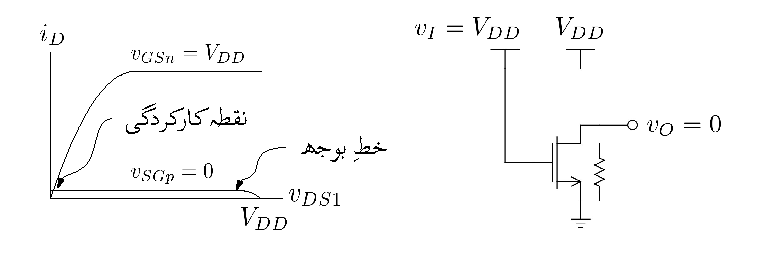
\includegraphics[scale=0.90]{NOTgateHighInput}
\caption{داخلی اشارہ بلند ہونے کی صورت میں خارجی اشارہ پست حاصل ہوتا ہے۔}
\label{شکل_ماسفیٹ_نفی_کار_داخلی_بلند_خارجی_پست}
\end{figure}

\عددیء{v_I=0} کی صورت میں \عددیء{v_{DS}=V_{DD}} جبکہ \عددیء{i_D \approx 0} کے برابر حاصل ہوتا ہے لہٰذا \عددیء{Q_n} میں برقی طاقت کا ضیاع قابل نظر انداز ہو گا۔چونکہ اس صورت میں \عددیء{V_{SD} \approx 0} ہے لہٰذا \عددیء{Q_p} میں طاقت کا ضیاع اس سے بھی کم ہو گا۔\عددیء{v_I=V_{DD}} کی صورت میں \عددیء{Q_n} اور \عددیء{Q_p} کے کردار آپس میں تبدیل ہو جاتے ہیں لہٰذا طاقت کا ضیاع جوں کا توں رہتا ہے۔حقیقت میں ماسفیٹ سے بنائے نفی کار میں کل طاقت کا ضیاع ایک مائیکرو واٹ سے بھی کم ہوتا ہے۔ 

آئیں شکل \حوالہ{شکل_ماسفیٹ_نفی_کار_الف} میں دئے نفی کار کا \عددیء{v_O} بالمقابل \عددیء{v_I} خط حاصل کریں۔ایسا کرنے کی خاطر \عددیء{v_I} کو بتدریج \عددیء{\SI{0}{\volt}} سے  \عددیء{V_{DD}} تک  تبدیل کرتے ہوئے \عددیء{v_O} حاصل کیا جائے گا۔پہلے  دونوں ماسفیٹ کے برقی رو بالمقابل برقی دباو مساوات  لکھتے ہیں۔

شکل سے \عددیء{Q_n} کے لئے \عددیء{v_{GS}=v_I} اور \عددیء{v_{DS}=v_O} لکھا جا سکتا ہے۔یوں  مساوات \حوالہ{مساوات_میدانی_غیر_افزائندہ_خطے_کی_نشاندہی} اور مساوات \حوالہ{مساوات_میدانی_غیر_افزائندہ_رو} کو یوں لکھا جا سکتا ہے۔
\begin{align}\label{مساوات_ماسفیٹ_نفی_کار_کے_ماسفیٹ_مساوات_الف}
i_{DS}=k_n \left[\left(v_{I}-V_{tn} \right )v_{O}-\frac{v_{O}^{2}}{2} \right ] \hspace{5mm} \textrm{جب}  \hspace{1.5mm} v_O \le v_I-V_{tn}
\end{align}
اسی طرح مساوات \حوالہ{مساوات_میدانی_افزائندہ_خطے_کی_نشاندہی} اور مساوات \حوالہ{مساوات_میدانی_افزائندہ_رو} کو
\begin{align}\label{مساوات_ماسفیٹ_نفی_کار_کے_ماسفیٹ_مساوات_ب}
i_{DS}=\frac{k_n}{2} \left[v_{I}-V_{tn} \right]^{2}  \hspace{5mm} \textrm{جب}  \hspace{1.5mm} v_O \ge v_I-V_{tn}
\end{align}
لکھا جا سکتا ہے۔اسی طرح \عددیء{Q_p} کے لئے مساوات \حوالہ{مساوات_ماسفیٹ_جمع_غیر_افزائندہ_حدود_و_مساوات} کو 
\begin{align}\label{مساوات_ماسفیٹ_نفی_کار_کے_ماسفیٹ_مساوات_پ}
i_{SD}&=k_p \left[\left(V_{DD}-v_I+V_{tp} \right )\left(V_{DD}-v_O\right)-\frac{\left(V_{DD}-v_O \right)^{2}}{2} \right ] \hspace{5mm} \textrm{جب}  \hspace{1.5mm} v_O \ge v_I-V_{tp}
\end{align}
اور مساوات \حوالہ{مساوات_ماسفیٹ_منفی_ماسفیٹ_افزائنہ_صورت_مثبت_متغیرات} کو
\begin{align}\label{مساوات_ماسفیٹ_نفی_کار_کے_ماسفیٹ_مساوات_ت}
i_{SD}&=\frac{k_p}{2} \left[V_{DD}-v_I+V_{tp} \right]^{2} \hspace{5mm} \textrm{جب}  \hspace{1.5mm} v_O \le v_I-V_{tp}
\end{align}
لکھا جا سکتا ہے۔نفی کار کو عموماً یوں تخلیق دیا جاتا ہے کہ
\begin{align}\label{مساوات_ماسفیٹ_نفی_کار_متشاکل_ہونے_کے_شرط}
V_{tn}&=\abs{V_{tp}}=V_t\\
k_n&=k_p
\end{align}
 ہوں۔اس طرح \عددیء{v_O} بالمقابل \عددیء{v_I} کا خط متشاکل تناسب رکھتا ہے اور خارجی سرے پر \عددیء{v_O} کی پست اور بلند دونوں صورتوں میں نفی کار یکساں برقی رو کی صلاحیت رکھتا ہے۔مندرجہ بالا چار مساوات سے شکل \حوالہ{شکل_ماسفیٹ_نفی_کار_خارجی_بالمقابل_داخلی_خط} میں دکھایا گیا خط حاصل ہوتا ہے۔عددی ادوار کے نقطہ نظر سے غالباً اس خط سے زیادہ اہم کوئی خط نہیں پایا جاتا لہٰذا اس کو اچھی طرح سمجھ کر ہی آگے بڑھیں۔آئیں اس پر خط مزید غور کریں۔
\begin{figure}
\centering
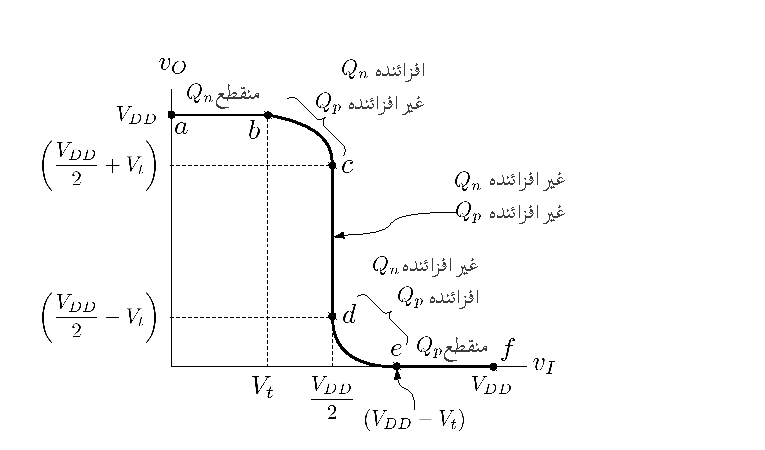
\includegraphics[scale=0.90]{NOTgateCMOScharacteristics}
\caption{نفی کار کا خط}
\label{شکل_ماسفیٹ_نفی_کار_خارجی_بالمقابل_داخلی_خط}
\end{figure}

شکل \حوالہ{شکل_ماسفیٹ_نفی_کار_خارجی_بالمقابل_داخلی_خط} پر اہم نقطے دکھائے گئے ہیں۔تصور کریں کہ \عددیء{V_t=\SI{1}{\volt}} اور \عددیء{V_{DD}=\SI{5}{\volt}} ہیں۔اس طرح \عددیء{V_{tn}=\SI{1}{\volt}} اور \عددیء{V_{tp}=\SI{-1}{\volt}} ہوں  گے۔شکل میں \عددیء{a} تا \عددی{b} خطے پر غور کریں۔یہاں \عددیء{v_I} کی قیمت \عددیء{\SI{0}{\volt}} تا \عددیء{\SI{1}{\volt}} ہے۔چونکہ \عددیء{Q_n} کی \عددیء{v_{GS}=v_I} ہے  لہٰذا \عددیء{v_{GS} < V_{tn}} ہے۔یوں \عددیء{Q_n} منقطع ہے۔اس کے برعکس \عددیء{Q_p} کی \عددیء{v_{SG}=V_{DD}-v_I} ہے لہٰذا \عددیء{v_{SG}} کی قیمت \عددیء{\SI{5}{\volt}} تا \عددیء{\SI{4}{\volt}} رہے گی۔چونکہ \عددیء{V_{tp}=\SI{-1}{\volt}} ہے لہٰذا \عددیء{-V_{tp}=\SI{1}{\volt}} ہو گا اور اس طرح \عددیء{v_{SG} > -V_{tp}} ہے۔ اس طرح  \عددیء{Q_p} چالو ہے۔مزید \عددیء{v_O=\SI{5}{\volt}} ہے لہٰذا اسی ماسفیٹ کے  \عددیء{v_{GD}} کی قیمت \عددیء{\SI{-4}{\volt}} تا \عددیء{\SI{-5}{\volt}} رہے گی  جو \عددیء{V_{tp}} سے کم ہے لہٰذا \عددیء{Q_p} غیر افزائندہ ہو گا۔ 

شکل \حوالہ{شکل_ماسفیٹ_نفی_کار_خارجی_بالمقابل_داخلی_خط} سے \عددیء{v_I} اور \عددیء{v_O}  کی قیمتیں پڑھتے ہوئے تسلی کر لیں کہ \عددیء{b} تا \عددیء{c} منفی ماسفیٹ افزائندہ جبکہ مثبت ماسفیٹ غیر افزائندہ ہے۔بقایا نقطوں کے درمیان بھی صورت حال دیکھیں۔ 
%=================
\حصہ{جوڑدار فیٹ \عددی{(JFET)}}
جوڑدار فیٹ کے دو اقسام یعنی \عددی{n} اور \عددی{p} پائے جاتے ہیں۔شکل \حوالہ{شکل_جوڑدار_منفی_فیٹ_ساخت} میں \عددی{n} قسم کے جوڑدار فیٹ یعنی \عددی{(nJFET)} کی ساخت اور علامت دکھائے گئے ہیں۔منفی جوڑدار فیٹ بنانے کی خاطر \عددی{n} قسم سلیکان ٹکڑے کے دونوں اطراف \عددی{p} قسم کے خطے بنائے جاتے ہیں جنہیں گیٹ\حاشیہب{gate} کہتے ہیں۔ان دو خطوں کو بیرونی دھاتی تار سے جوڑ کر بطور گیٹ \عددی{(G)} استعمال کیا جاتا ہے۔شکل میں اس بیرونی دھاتی تار کو نہیں دکھایا گیا ہے۔دو گیٹوں کے درمیان راہ میں آزاد الیکٹران پائے جاتے ہیں۔اس راہ پر بیرونی برقی دباو \عددی{v_{DS}} لاگو کرنے سے راہ میں موجود آزاد الیکٹران منفی برقی دباو والے سرے سے مثبت برقی دباو والے سرے کی جانب حرکت کریں گے جس سے برقی رو \عددی{i_{DS}} پیدا ہو گی۔یوں منفی برقی دباو والے سرے سے خارج الیکٹران، مثبت برقی دباو والے سرے پر حاصل ہوتے ہیں۔اسی سے ان دو سروں کو سورس \عددی{S} اور ڈرین \عددی{D} کے نام دئے گئے ہیں۔روایتی برقی رو الیکٹران کے حرکت کی الٹ سمت ہوتی ہے۔یوں \عددی{(nJFET)} میں روایتی برقی رو کی سمت راہ میں ڈرین سے سورس کی جانب ہو گی۔ اگرچہ راہ میں برقی رو دونوں جانب بالکل یکساں طور ممکن ہے اور یوں اس کے سروں کو \عددی{S} اور \عددی{D} کے نام دینا شاید درست نہ لگے ہم پھر بھی اس راہ کے ایک سرے کو سورس \عددی{(S)} جبکہ دوسرے سرے کو ڈرین \عددی{(D)} پکاریں گے۔بیرونی برقی دباو کا مثبت سرا \عددی{(nJFET)} کے \عددی{D} کی جانب رکھا جائے گا۔\تحریر{nJFET} میں راہ \عددی{n} قسم کے نیم موصل سے حاصل ہوتا ہے اور اس کے نام میں \عددی{n} اسی  کو ظاہر کرتا ہے۔

\begin{figure}
\centering
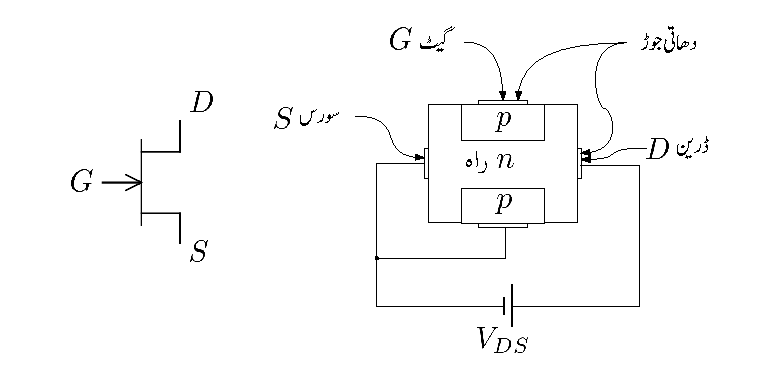
\includegraphics[scale=0.90]{nJFETstructure}
\caption{جوڑدار منفی فیٹ کی ساخت}
\label{شکل_جوڑدار_منفی_فیٹ_ساخت}
\end{figure}
آئیں شکل \حوالہ{شکل_جوڑدار_منفی_فیٹ_کارکردگی} کی مدد سے \تحریر{nJFET} کی کارکردگی پر غور کریں۔راہ اور گیٹ آپس میں \عددی{pn} جوڑ یعنی ڈایوڈ بناتے ہیں۔\تحریر{nJFET} کی علامت میں گیٹ پر تیر کا نشان اس ڈایوڈ کے سیدھے رخ کو دکھاتا ہے۔اس جوڑ پر بالکل ڈایوڈ کی طرح ویران خطہ وجود میں آتا ہے اور جیسا کہ آپ جانتے ہیں، اس ویران خطے کی چوڑائی کا دارومدار اس جوڑ پر پائے جانے والے برقی دباو پر ہے۔شکل  الف میں سورس \عددی{S} کو برقی زمین پر رکھتے  ہوئے گیٹ \عددی{G} پر منفی برقی دباو لاگو کیا گیا ہے۔گیٹ پر لاگو منفی برقی دباو کو جتنا زیادہ منفی کیا جائے ویران خطہ اتنا ہی زیادہ چوڑا ہو گا اور \عددی{n} راہ کی چوڑائی اتنی ہی کم ہو گی۔\عددی{v_{GS}} کو اگر بتدریج منفی جانب بڑھایا جائے تو ویران خطہ بڑھتے بڑھتے آخر کار تمام \عددی{n} راہ کو گھیر لے گا۔جس \عددی{v_{GS}} پر ایسا ہو، اس کو \تحریر{nJFET} کے دبوچنے کا برقی دباو کہتے ہیں اور روایتی طور اسے \عددی{V_p} سے ظاہر کیا جاتا ہے۔یوں  \تحریر{nJFET} کے \عددی{V_p} کی قیمت منفی ہو گی۔اس سے معلوم یہ ہوا کہ راہ کی گہرائی کو گیٹ پر برقی دباو سے قابو کیا جا سکتا ہے۔مزید یہ کہ گیٹ اور راہ \عددی{pn} جوڑ بناتے ہیں۔اگر گیٹ اور راہ کے درمیان مثبت برقی دباو دی جائے تو راہ کی گہرائی مزید نہیں بڑھ سکتی بلکہ گیٹ اور راہ کے مابین \عددی{pn} جوڑ سیدھا مائل ہو جائے گا اور اس میں برقی رو گزرنے شروع ہو جائے گی۔یوں آپ دیکھ سکتے ہیں کہ \تحریر{nJFET} میں گیٹ اور راہ کے درمیان برقی دباو کو \عددی{pn} جوڑ کے چالو برقی دباو \عددی{\SI{0.5}{\volt}} سے کم ہی رکھا جاتا ہے۔

\عددی{D} اور \عددی{S} کے مابین راہ بالکل ایک موصل سلاخ کی مانند مزاحمت کا کردار ادا کرے گا۔یوں اگر راہ کی لمبائی \عددیء{L}، گہرائی \عددیء{g}، چوڑائی \عددی{W} اور اس کے موصلیت کا مستقل \عددی{\sigma} ہو تو اس کا مزاحمت \عددی{R=\frac{L}{\sigma Wg}}  ہو گا۔

اب تصور کریں کہ ڈرین \عددی{D} پر معمولی مثبت برقی دباو \عددی{v_{DS}} لاگو کیا جاتا ہے۔\عددی{n} راہ میں برقی رو \عددی{i_{DS}} گزرے گی جس کی قیمت اُوہم کے قانون سے حاصل کی جا سکتی ہے۔\عددی{v_{DS}} کو کم یا زیادہ کرتے ہوئے \عددی{i_{DS}} کو کم یا زیادہ کرنا ممکن ہے۔کم \عددی{v_{DS}} پر، کسی بھی مزاحمت کی طرح، برقی دباو بالمقابل برقی رو کا خط تقریباً سیدھا ہو گا۔اب تصور کریں کہ \عددی{v_{GS}} کو تبدیل کئے بغیر \عددی{v_{DS}} کو بڑھایا جائے۔یوں \عددی{n} راہ کے سورس سرے پر \عددی{0 V} جبکہ اس کے ڈرین سرے پر \عددی{v_{DS}} برقی دباو پائی جائے گی۔جیسا شکل  ب میں دکھایا گیا ہے، یوں سورس سرے کے قریب \عددی{pn} جوڑ پر ویران خطے کی چوڑائی کم جبکہ ڈرین سرے کے قریب ویران خطے کی چوڑائی زیادہ ہو گی۔ان دو سروں کے درمیان ویران خطے کی چوڑائی ترچھی شکل اختیار کرے گی۔اس ترچھا پن کی وجہ سے \عددی{n} راہ کی مزاحمت بڑھے گی جس سے راہ کا مزاحمت بھی بڑھے گا۔یوں اگرچہ کم \عددی{v_{DS}} پر \عددی{v_{DS}-i_{DS}} کا خط سیدھا ہو گا لیکن جیسے جیسے \عددی{v_{DS}} بڑھایا جائے، راہ کا مزاحمت ایسے ایسے بڑھے گا اور یوں \عددی{v_{DS}-i_{DS}} کے خط میں جھکاو پیدا ہو گا۔اگر  \عددی{v_{DS}} کو بتدریج بڑھایا جائے تو آخر کار ڈرین سرے کی جانب ویران خطہ بڑھتے بڑھتے راہ کو دبوچ جائے گا۔شکل  ب میں ایسا ہوتے دکھایا گیا ہے۔\عددی{v_{DS}} کو مزید بڑھانے سے برقی رو میں تبدیلی نہیں پیدا ہوتی اور اس کی قیمت نقطہ دبوچ پر پائے جانے والے برقی رو کے قیمت پر ہی رہتی ہے۔

مندرجہ بالا تذکرے سے ظاہر ہے کہ \تحریر{JFET} بالکل گھٹاتا ماسفیٹ کی مانند کام کرتا ہے۔البتہ جہاں ماسفیٹ کے گیٹ پر مثبت یا منفی برقی دباو دینا ممکن ہے، \تحریر{nJFET} کے گیٹ پر صرف منفی برقی دباو ہی دینا ممکن ہے۔اگر اس کے گیٹ پر مثبت برقی دباو دی جائے تو گیٹ اور راہ کے مابین \عددی{pn} جوڑ یعنی یہاں کا ڈایوڈ سیدھا مائل ہو جائے گا اور گیٹ \تحریر{nJFET} کو قابو کرنے کی صلاحیت کھو دے گا۔چونکہ \تحریر{JFET} کے گیٹ پر ڈایوڈ کو الٹا مائل رکھا جاتا ہے لہٰذا اس کے گیٹ پر نہایت کم (الٹے مائل ڈایوڈ کے برابر) برقی رو پائی جاتی ہے جسے عموماً صفر ایمپیئر تصور کیا جاتا ہے۔یہ برقی رو اگرچہ نہایت کم ہے لیکن ماسفیٹ کے گیٹ پر اس سے بھی کئی درجے کم برقی رو پائی جاتی ہے۔
\begin{figure}
\centering
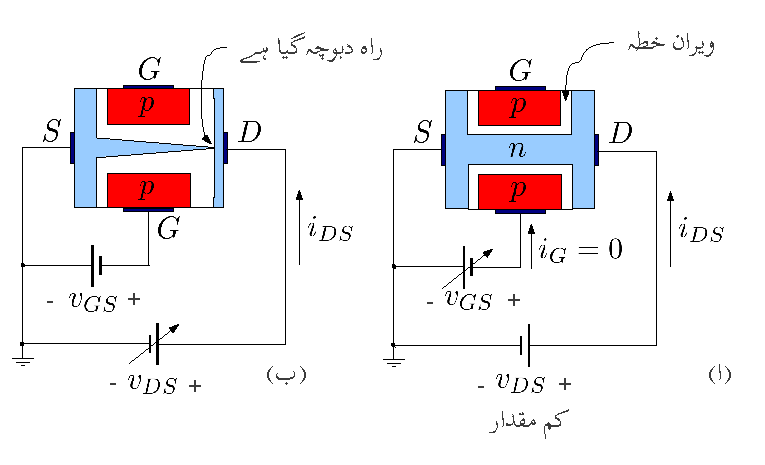
\includegraphics[scale=0.90]{nJFEToperation}
\caption{جوڑدار منفی فیٹ کی کارکردگی}
\label{شکل_جوڑدار_منفی_فیٹ_کارکردگی}
\end{figure}

\جزوحصہ{برقی رو بالمقابل برقی دباو}
چونکہ \تحریر{JFET} کی کارکردگی بالکل گھٹاتا ماسفیٹ کی مانند ہے لہٰذا گھٹاتا ماسفیٹ کے مساوات ہی  \تحریر{JFET} کے لئے بھی  استعمال کئے جائیں گے۔البتہ  ادب میں \تحریر{JFET} کے مساوات کو قدر مختلف طریقے سے لکھا جاتا ہے۔آئیں \تحریر{nJFET} کے مساوات دیکھیں۔

\جزوجزوحصہ{منقطع خطہ}
جیسا کہ اوپر ذکر کیا گیا، اگر \عددی{v_{GS}} کو \عددی{V_p} سے کم کیا جائے تو ویران خطہ تمام راہ کو گھیر لیتا ہے اور برقی رو کا گزر ممکن نہیں ہوتا یعنی
\begin{align}
v_{GS} \le V_p   \hspace{2 cm}  i_D=0 
\end{align}

\جزوجزوحصہ{غیر افزائندہ خطہ}
غیر افزائندہ خطے میں \عددی{pn} جوڑ کو الٹا مائل رکھتے ہوئے \عددی{v_{GS}} کو \عددی{V_p} سے زیادہ رکھا جاتا ہے۔مزید یہ کہ \عددی{v_{DS}} کو نقطہ دبوچ سے کم رکھا جاتا ہے۔اس خطے میں ماسفیٹ کی مساوات \حوالہ{مساوات_میدانی_غیر_افزائندہ_رو} کو \تحریر{JFET} کے لئے  یہاں لکھتے ہیں۔ایسا کرتے ہوئے \عددی{V_t} کی جگہ \عددی{V_p} لکھا جائے گا۔
 \begin{align*}
i_{DS} &=k_n \left[ (v_{GS}-V_p) v_{DS}-\frac{v_{DS}^2}{2} \right] \\
&=\frac{k_n V_p^2}{2} \left[ 2 \left(\frac{v_{GS}}{V_p}-1 \right)  \frac{v_{DS}}{V_p}-\left(\frac{v_{DS}}{V_p} \right)^2 \right]
\end{align*}
اس مساوات میں \عددی{\frac{k_n V_p^2}{2}} کو \تحریر{JFET} کے لئے \عددی{I_{DSS}} لکھا جاتا ہے۔ یوں
\begin{gather}
\begin{aligned} \label{مساوات_منفی_فیٹ_غیر_افزائندہ}
V_p \le v_{GS} \le 0, \hspace{2 cm} v_{DS} \le v_{GS}-V_p \\
i_{DS}=I_{DSS} \left[ 2 \left(\frac{v_{GS}}{V_p}-1 \right)  \frac{v_{DS}}{V_p}-\left(\frac{v_{DS}}{V_p} \right)^2 \right]
\end{aligned}
\end{gather}

\جزوجزوحصہ{افزائندہ خطہ}
ماسفیٹ کی مساوات \حوالہ{مساوات_میدانی_افزائندہ_رو} کو یوں لکھا جاتا ہے۔
\begin{gather}
\begin{aligned} \label{مساوات_منفی_فیٹ_افزائندہ}
V_p \le v_{GS} \le 0, \hspace{2 cm} v_{DS} \ge v_{GS}-V_p\\
i_{DS}=I_{DSS} \left(1-\frac{v_{GS}}{V_p} \right)^2 \left(1+\frac{v_{DS}}{V_A} \right)
\end{aligned}
\end{gather}
جہاں ارلی برقی دباو \عددی{V_A}\حاشیہب{Early Voltage} کے اثر کو بھی شامل کیا گیا ہے۔ارلی برقی دباو کے اثر کو نظر انداز کرتے ہوئے، \عددی{v_{GS}=0} پر اس مساوات سے \عددی{i_{DS}=I_{DSS}} حاصل ہوتا ہے لہٰذا \عددی{I_{DSS}} وہ برقی رو ہے جو گیٹ کو سورس کے ساتھ جوڑنے سے حاصل ہوتی ہے۔ مندرجہ بالا مساوات میں \عددی{(v_{DS} \ge v_{GS}-V_p)}  کو \عددی{(v_{GS}-v_{DS} \le V_p)} یا \عددی{(v_{GD} \le V_p)} بھی لکھا جا سکتا ہے۔

%==========
\جزوحصہ{\تحریر{pJFET}}
جیسا شکل \حوالہ{شکل_جوڑدار_مثبت_فیٹ_ساخت} الف میں دکھایا گیا ہے، مثبت جوڑدار فیٹ بنانے کی خاطر \عددی{p} قسم سلیکان ٹکڑے کے دونوں اطراف \عددی{n} گیٹ بنائے جاتے ہیں۔ان دو خطوں کو بیرونی دھاتی تار سے جوڑ کر بطور  گیٹ \عددی{(G)} استعمال کیا جاتا ہے۔دو گیٹوں کے درمیان راہ میں آزاد خول پائے جاتے ہیں۔اس راہ پر بیرونی برقی دباو \عددی{v_{SD}} لاگو کرنے سے راہ میں موجود آزاد خول مثبت برقی دباو والے سرے سے منفی برقی دباو والے سرے کی جانب حرکت کریں گے جس سے برقی رو \عددی{i_{SD}} پیدا ہو گی۔یوں مثبت برقی دباو والے سرے سے خارج خول، منفی برقی دباو والے سرے پر حاصل ہوتے ہیں۔اسی سے ان دو سروں کو سورس \عددی{S} اور ڈرین \عددی{D} کے نام دئے گئے ہیں۔یوں \عددی{(pJFET)} میں روایتی برقی رو کی سمت راہ میں سورس سے ڈرین کی جانب ہو گی۔بیرونی برقی دباو کا مثبت سرا \عددی{(pJFET)} کے \عددی{S} کی جانب رکھا جائے گا۔\تحریر{pJFET} میں راہ \عددی{p} قسم کے نیم موصل سے حاصل ہوتا ہے اور اس کے نام میں \عددی{p} اسی  کو ظاہر کرتا ہے۔جیسا شکل \حوالہ{شکل_جوڑدار_مثبت_فیٹ_ساخت} ب میں دکھایا گیا ہے، \تحریر{pJFET} کی علامت میں گیٹ پر تیر کا نشان راہ سے گیٹ کی جانب کو ہوتا ہے۔\تحریر{pJFET} کی صحیح کارکردگی کے لئے ضروری ہے کہ گیٹ اور راہ پر بننے والے \عددی{pn} جوڑ کو غیر چالو رکھا جائے یعنی اس جوڑ پر ڈایوڈ کے سیدھے رخ \عددی{\SI{0.5}{\volt}} سے برقی دباو کو کم رکھا جائے۔
\begin{figure}
\centering
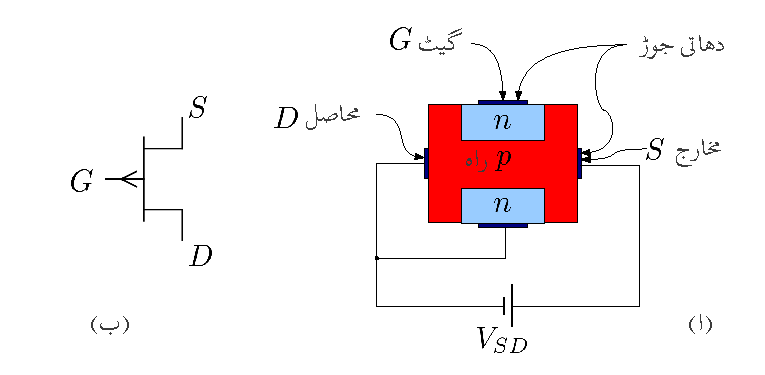
\includegraphics[scale=0.90]{pJFETstructure}
\caption{جوڑدار مثبت فیٹ کی ساخت}
\label{شکل_جوڑدار_مثبت_فیٹ_ساخت}
\end{figure}
\جزوحصہ{باریک اشاراتی ماڈل}
چونکہ \تحریر{JFET} اور \تحریر{MOSFET} کی کارکردگی یکساں ہے لہٰذا ان کے پست تعددی اور بلند تعددی پائے ماڈل بھی یکساں ہیں۔یہاں
\begin{align} \label{مساوات_افزائش_فیٹ}
g_m &=\left(\frac{-2  I_{DSS}}{V_p} \right) \left(1-\frac{V_{GS}}{V_p} \right) \\
&=\left(\frac{-2  I_{DSS}}{V_p} \right)  \sqrt{\frac{I_D}{I_{DSS}}}
\end{align} 
کے برابر ہے جہاں \عددی{I_D} نقطہ مائل پر یک سمتی برقی رو ہے۔اسی طرح
\begin{align}
r_o=\frac{V_A}{I_D}
\end{align} 
کے برابر ہے۔
%==================
\ابتدا{مثال}
ایک \تحریر{nJFET} کے \عددی{V_p=\SI{-3}{\volt}} اور \عددی{I_{DSS}=\SI{8}{\milli \ampere}} ہیں۔اس کی برقی رو \عددی{v_{GS}=\SI{-1.5}{\volt}} اور \عددی{v_{DS}=\SI{3.5}{\volt}} پر حاصل کریں۔ارلی برقی دباو کے اثر کو نظر انداز کریں۔

حل:چونکہ \عددی{v_{GS}-V_p} کی قیمت 
\begin{align*}
(\SI{-1.5}{\volt})-(\SI{-3}{\volt})=\SI{1.5}{\volt}
\end{align*}
دئے گئے \عددی{v_{DS}} کے قیمت سے کم ہے لہٰذا مساوات \حوالہ{مساوات_منفی_فیٹ_افزائندہ} کے پہلے جزو کے تحت فیٹ افزائندہ خطے میں ہے اور یوں اسی مساوات کے دوسرے جزو کے تحت
\begin{align*}
i_{DS}=8 \times 10^{-3} \left[1-\left(\frac{-1.5}{-3} \right) \right]^2= \SI{2}{\milli \ampere}
\end{align*}
حاصل ہوتا ہے۔
\انتہا{مثال}
%====================
\ابتدا{مثال}
مندرجہ بالا مثال میں \عددی{v_{GS}} کو بڑھا کر  \عددی{\SI{-1.4}{\volt}} کر دیا جاتا ہے۔\عددی{i_{DS}} میں تبدیلی حاصل کرتے ہوئے \عددی{\frac{\Delta i_{DS}}{\Delta v_{GS}}} حاصل کریں۔مساوات \حوالہ{مساوات_افزائش_فیٹ} سے \عددی{g_m} کی قیمت حاصل کرتے ہوئے دونوں جوابات کا موازنہ کریں۔

حل:اب بھی \عددی{(v_{DS} \ge v_{GS}-V_p)} ہے لہٰذا
\begin{align*}
i_{DS}=8 \times 10^{-3} \left[1-\left(\frac{-1.4}{-3} \right) \right]^2= \SI{2.2756}{\milli \ampere}
\end{align*}
حاصل ہوتا ہے جس سے
\begin{align*}
\frac{\Delta i_{DS}}{\Delta v_{GS}}=\frac{\SI{2.2756}{mA}-\SI{2}{mA}}{(-1.4)-(-1.5)}=\SI[per=frac,fraction=nice]{2.756}{\milli \ampere \per \volt}
\end{align*}
حاصل ہوتا ہے۔مساوات \حوالہ{مساوات_افزائش_فیٹ} کے تحت
\begin{align*}
g_m=\left(\frac{-2 \times \SI{8}{mA}}{-3} \right) \sqrt{\frac{\SI{2}{mA}}{\SI{8}{mA}}}=\SI{2.6667}{mA}
\end{align*} 
حاصل ہوتا ہے۔ان دونوں جوابات میں صرف
\begin{align*}
\left(\frac{2.756-2.6667}{2.6667} \right) \times 100=\SI{3.34}{\percent}
\end{align*}
کا فرق ہے۔\عددی{v_{GS}} میں تبدیلی کو کم سے کم کرتے ہوئے زیادہ درست جواب حاصل ہوتا ہے۔  
\انتہا{مثال}

\ابتدا{مثال}
ارلی برقی دباو \عددی{V_A} کی قیمت \عددی{\SI{75}{\volt}} لیتے ہوئے خارجی مزاحمت \عددی{r_o} کا تخمینہ \عددی{\SI{1}{\milli \ampere}} اور \عددی{\SI{10}{\milli \ampere}} پر لگائیں۔ایسا کرتے ہوئے تصور کریں کہ فیٹ افزائندہ خطے میں ہے۔

حل:ایک ملی ایمپیئر پر
\begin{align*}
r_o=\frac{75}{0.001}=\SI{75}{\kilo \ohm}
\end{align*}
اور دس ملی ایمپیئر پر
\begin{align*}
r_o=\frac{75}{0.01}=\SI{7.5}{\kilo \ohm}
\end{align*}
حاصل ہوتا ہے۔
\انتہا{مثال}

\ابتدا{مثال}
شکل \حوالہ{شکل_جوڑدار_منفی_فیٹ_مثال} میں منفی جوڑدار فیٹ کا ایمپلیفائر دکھایا گیا ہے جس میں استعمال ہونے والے فیٹ کی \عددی{V_p=\SI{-3}{\volt}} اور \عددی{I_{DSS}=\SI{8}{\milli \ampere}} ہیں۔\عددی{V_{DD}=\SI{15}{\volt}} تصور کرتے ہوئے برقی رو \عددیء{I_{DS}=\SI{5}{\milli \ampere}}، \عددی{V_G=\SI{4}{\volt}} جبکہ \عددی{V_D=\SI{9}{\volt}} حاصل کرنے کی خاطر درکار مزاحمت معلوم کریں۔ایسا کرتے وقت گیٹ پر نسب مزاحمت میں \عددی{\SI{10}{\micro \ampere}} کی برقی رو تصور کریں۔تمام کپیسٹروں کی قیمت لامحدود تصور کرتے ہوئے ایمپلیفائر کی افزائش \عددی{A_v} حاصل کریں۔ایمپلیفائر کی داخلی مزاحمت \عددی{R_i} اور خارجی مزاحمت \عددی{R_o} بھی حاصل کریں۔

\begin{figure}
\centering
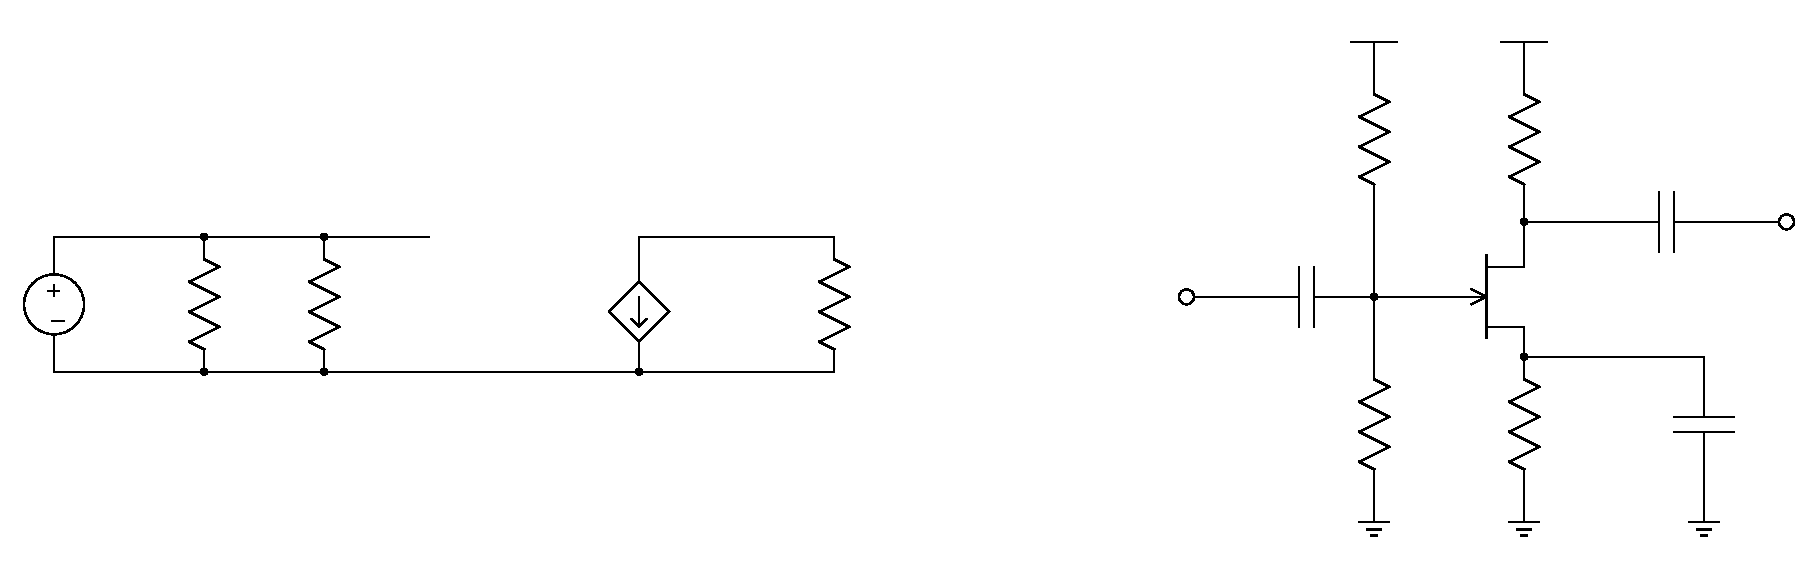
\includegraphics[scale=0.90]{nJFETexampleA}
\caption{جوڑدار منفی فیٹ کی مثال}
\label{شکل_جوڑدار_منفی_فیٹ_مثال}
\end{figure}

حل:
گیٹ کے مزاحمت میں \عددی{\SI{10}{\micro A}} برقی رو ہے۔یوں
\begin{align*}
\frac{V_{DD}}{R_1+R_2} &=\SI{10}{\micro A} \\
R_1+R_2&=\frac{15}{10 \times 10^{-6}}=\SI{1.5}{M \ohm}
\end{align*}
حاصل ہوتا ہے۔گیٹ پر \عددی{\SI{4}{V}} حاصل کرنے کی خاطر
\begin{align*}
V_G&=\left(\frac{R_1}{R_1+R_2} \right) V_{DD} \\
4&=\left(\frac{R_1}{1.5 \times 10^6}\right) \times 15 \\
R_1&=\SI{400}{k \ohm}
\end{align*}
حاصل ہوتا ہے۔یوں
\begin{align*}
R_2=\SI{1.5}{M \ohm}-\SI{400}{k \ohm}=\SI{1.1}{M \ohm}
\end{align*}
حاصل ہوتا ہے۔\عددی{V_D=\SI{9}{V}} کی خاطر
\begin{align*}
V_{DD}-V_D&=I_{DS} R_D \\
R_D &=\frac{15-9}{5 \times 10^{-3}}=\SI{1.2}{k \ohm}
\end{align*}
حاصل ہوتا ہے۔

چونکہ \عددی{(V_{G}-V_{D}=4-9=-5)} ہے جو کہ \عددی{V_p} سے کم ہے لہٰذا فیٹ افزائندہ خطے میں ہے۔یوں مساوات \حوالہ{مساوات_منفی_فیٹ_افزائندہ} کے تحت
\begin{align*}
5 \times 10^{-3}&=8 \times 10^{-3} \left(1-\frac{V_{GS}}{-3} \right)^2 \\
V_{GS}&=\SI{-0.628}{V}
\end{align*}
یعنی
\begin{align*}
V_{GS}&=V_G-V_S=\SI{-0.628}{V} \\
V_S&=\SI{4.628}{V}
\end{align*}
حاصل ہوتا ہے۔جس سے
\begin{align*}
V_S &=I_{DS} R_S \\
R_S&=\frac{4.628}{5 \times 10^{-3}}=\SI{925}{\ohm}
\end{align*}
حاصل ہوتا ہے۔

شکل  ب میں مساوی باریک اشاراتی دور دکھایا گیا ہے جس سے
\begin{align*}
R_i&=\frac{R_1 R_2}{R_1+R_2}=\SI{293}{k \ohm}\\
R_o&=R_D=\SI{1.2}{k \ohm}
\end{align*}
حاصل ہوتے ہیں۔آپ دیکھ سکتے ہیں کہ \عددی{R_i} کا دارومدار گیٹ پر نسب مزاحمتوں پر ہے۔یوں داخلی مزاحمت بڑھانے کی خاطر ان مزاحمتوں کو زیادہ سے زیادہ رکھا جاتا ہے جس کا مطلب ہے کہ ان میں گزرتے یک سمتی رو کو کم سے کم رکھا جاتا ہے۔اس مثال میں اس برقی رو کو \عددی{\SI{10}{\micro \ampere}}  رکھا گیا ہے۔

مساوات \حوالہ{مساوات_افزائش_فیٹ} کی مدد سے
\begin{align*}
g_m=\frac{-2 \times 8 \times 10^{-3}}{-3} \sqrt{\frac{5 \times 10^{3}}{8 \times 10^{-3}}}=\SI[per=frac,fraction=nice]{4.216}{\milli \ampere \per \volt}
\end{align*}
اور یوں
\begin{align*}
A_v=\frac{v_o}{v_s}=-g_m R_D=-4.216 \times 10^{-3} \times 1.2 \times 10^3=\SI[per=frac,fraction=nice]{-5.059}{\volt \per \volt}
\end{align*}
حاصل ہوتا ہے۔
\انتہا{مثال}
%========================
\ابتدا{مثال}
شکل \حوالہ{شکل_ماسفیٹ_جمع_ماسفیٹ_مثال_درکار_مداخل} میں \عددی{v_L=2+0.56 \sin \omega t} اور \عددی{I_{SD}=\SI{1}{\milli \ampere}} ہیں۔\عددیء{R_D}، \عددیء{V_{GG}}، \عددیء{v_i} حاصل کرتے ہوئے \عددی{A_v=\tfrac{v_L}{v_i}} حاصل کریں۔ 

\begin{figure}
\centering
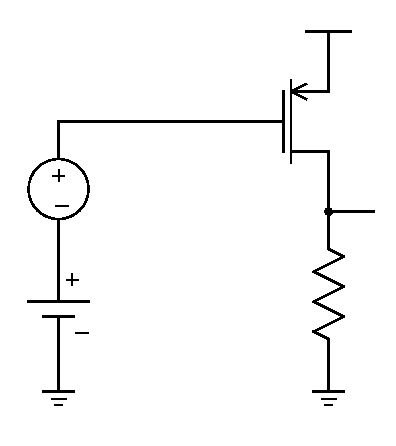
\includegraphics[scale=0.90]{pEnhancementExampleWithInputDefined}
\caption{}
\label{شکل_ماسفیٹ_جمع_ماسفیٹ_مثال_درکار_مداخل}
\end{figure}

حل:یک سمتی \عددی{v_L=\SI{2}{\volt}} ہے لہٰذا
\begin{align*}
R_D=\frac{2}{1 \times 10^{-3}}=\SI{2}{\kilo \ohm}
\end{align*}
ہے۔ماسفیٹ کو افزائندہ تصور کرتے ہوئے ماسفیٹ کی مساوات سے
\begin{align*}
10^{-3}=\frac{2 \times 10^{-3}}{2} \left( V_{SG}-1\right)^2
\end{align*}
سے \عددی{V_{SG}} کی قیمت \عددی{\SI{0}{\volt}} اور \عددی{\SI{2}{\volt}} حاصل ہوتے ہیں۔\عددی{V_t=\SI{-1}{\volt}} ہے لہٰذا \عددی{-V_t =\SI{1}{\volt}} کے برابر ہے۔\عددی{V_{SG} > -V_t} کی شرط سے \عددی{V_{SG}=\SI{2}{\volt}} کو درست جواب تسلیم کیا جاتا ہے۔یوں
\begin{align*}
V_{SG} &=V_S-V_G \\
2&=5-V_G
\end{align*}
سے \عددی{V_G=V_{GG}=\SI{3}{\volt}} حاصل ہوتا ہے۔
\begin{figure}
\centering
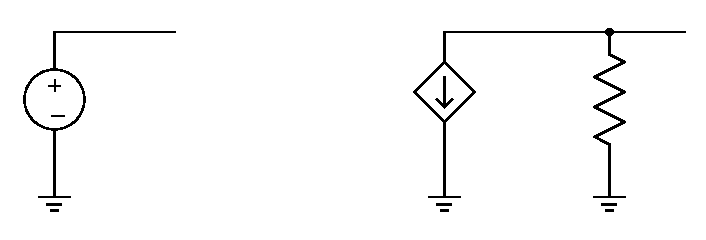
\includegraphics[scale=0.90]{pEnhancementExampleWithInputDefinedEquivalent}
\caption{}
\label{شکل_ماسفیٹ_جمع_ماسفیٹ_مثال_درکار_مداخل_الف}
\end{figure}
شکل \حوالہ{شکل_ماسفیٹ_جمع_ماسفیٹ_مثال_درکار_مداخل_الف} میں باریک اشاراتی مساوی دور دکھایا گیا ہے جسے دیکھ کر \عددی{v_L=-g_m v_{gs} R_D} لکھا جا سکتا ہے جہاں
\begin{align*}
g_m&=\sqrt{2 k_p I_{SD}}=\sqrt{2 \times 2 \times 10^{-3} \times 10^{-3}}=\SI{2}{\milli \siemens}\\
v_{gs}&=v_i
\end{align*}
کے برابر ہیں۔\عددی{v_L} میں بدلتا حصہ \عددی{0.56 \sin \omega t} ہے جسے استعمال کرتے ہوئے
\begin{align*}
0.56 \sin \omega t =-2 \times 10^{-3} v_i \times  2000
\end{align*}
سے \عددی{v_i=-0.14 \sin \omega t} اور \عددی{A_v=\SI{-4}{\volt \per \volt}} حاصل ہوتے ہیں۔
\انتہا{مثال}
%==========
\حصہ{مخلوط ادوار میں ماسفیٹ کا نقطہ کارکردگی تعین کرنے کے ادوار}
شکل \حوالہ{شکل_جوڑدار_منفی_فیٹ_مثال} اور \حوالہ{شکل_ماسفیٹ_ایمپلیفائر_الف} میں مزاحمت استعمال کرتے ہوئے انفرادی ماسفیٹ کا نقطہ کارکردگی  تعین کیا گیا۔مخلوط ادوار میں ماسفیٹ کا نقطہ کارکردگی مزاحمت استعمال کرتے ہوئے تعین نہیں کیا جاتا۔مخلوط دور بناتے وقت سلیکان پتری کے کم سے کم رقبے پر زیادہ سے زیادہ پرزے بنائے جاتے ہیں۔یوں مخلوط دور میں ان پرزوں کو ترجیح دی جاتی ہے جو کم سے کم رقبہ گھیریں۔ماسفیٹ کی نسبت سے مزاحمت زیادہ رقبہ گھیرتا ہے لہٰذا مزاحمت کے استعمال سے بچنے کی ہر ممکنہ  کوشش کی جاتی ہے۔مزید یہ کہ سلیکان پر بالکل درست قیمت کا مزاحمت بنانے کی خاطر اضافی گراں قیمت اقدام کرنے پڑتے ہیں جبکہ درکار خوبیوں کا ماسفیٹ آسانی سے  بنتا ہے۔اس کے علاوہ انفرادی ماسفیٹ ایمپلیفائر میں \اصطلاح {جفتی} اور \اصطلاح {متبادل راستہ} کپیسٹر استعمال کئے جاتے ہیں۔مخلوط دور میں چند \عددی{\si{\pico \farad}} سے زیادہ قیمت کا کپیسٹر بنانا ممکن نہیں ہوتا لہٰذا کپیسٹر کا استعمال بھی ممکن نہیں ہوتا۔آئیں دیکھیں کہ مخلوط دور میں ماسفیٹ کا نقطہ کارکردگی کیسے تعین کیا جاتا ہے۔
  
\جزوحصہ{منبع مستقل برقی رو}
شکل \حوالہ{شکل_ماسفیٹ_پیداکار_مستقل_برقی_رو} الف میں \اصطلاح {منبع مستقل برقی رو}\فرہنگ{منبع مستقل برقی رو}\حاشیہب{constant current source}\فرہنگ{constant current source} کا سادہ دور اور شکل  ب میں اس کی علامت دکھائے گئے ہیں۔مثال \حوالہ{مثال_میدانی_گیٹ_اور_محاصل_جڑے} کی طرح \عددی{Q_1} اور \عددی{R_{\textrm{حوالہ}}} کے دور کو حل کرنے سے برقی رو \عددی{I_{DS1}} اور برقی دباو \عددی{V_{DS1}=V_{GS1}} حاصل ہوں گے۔\عددی{Q_1} اور \عددی{Q_2} کے سورس آپس میں جڑے ہیں اور اسی طرح ان کے گیٹ بھی آپس میں جڑے ہیں لہٰذا ان دونوں کے \عددی{V_{GS}} برابر ہوں گے یعنی
\begin{align*}
V_{GS1}=V_{GS2}=V_{GS}
\end{align*}
ہو گا۔\عددی{Q_1} کا گیٹ اور ڈرین آپس میں جڑے ہیں لہٰذا اس کا \عددی{V_{GD} < V_t} ہے اور یہ افزائندہ خطے میں ہے لہٰذا
\begin{align}\label{مساوات_ماسفیٹ_مستقل_برقی_رو_الف}
I_{DS1}=\frac{k_n'}{2} \left(\frac{W}{L}\right)_1 \left(V_{GS}-V_t \right)^2
\end{align}
ہو گا۔گیٹ پر برقی رو صفر ہونے سے \عددی{I_{DS1}} اور \عددی{I_{\textrm{حوالہ}}} برابر ہوں گے۔یوں اُوہم کے قانون سے
\begin{align}\label{مساوات_ماسفیٹ_مستقل_برقی_رو_ب}
I_{DS1}=I_{\textrm{حوالہ}}=\frac{V_{DD}-V_{GS1}}{R_{\textrm{حوالہ}}}
\end{align}
لکھا جا سکتا ہے۔درکار \عددی{I_{DS1}} کے لئے دور میں مزاحمت \عددی{R_{\textrm{حوالہ}}} کی قیمت مندرجہ بالا دو مساوات حل کر کے  حاصل کی جاتی ہے۔

اگر ہم تصور کریں گے کہ \عددی{Q_2} بھی افزائندہ خطے میں ہے تب اس کے لئے ہم لکھ سکتے ہیں
\begin{align}
I_{DS2}=I_{\textrm{عکس}}=\frac{k_n'}{2} \left(\frac{W}{L}\right)_2 \left(V_{GS}-V_t \right)^2
\end{align} 
جہاں \عددی{V_{GS1}=V_{GS2}=V_{GS}} کے برابر ہے۔\عددی{I_{DS2}} کو \عددی{I_{DS1}} سے تقسیم کرتے ہوئے ملتا ہے
\begin{align}
\frac{I_{DS2}}{I_{DS1}}=\frac{I_{\textrm{عکس}}}{I_{\textrm{حوالہ}}}=\frac{\left(\frac{W}{L} \right)_2}{\left(\frac{W}{L} \right)_1}
\end{align}
آپ دیکھ سکتے ہیں کہ \عددی{I_{DS2}} کی قیمت کا دارومدار \عددی{I_{DS1}} کے قیمت کے حوالے سے ہے۔اگر دونوں ماسفیٹ بالکل ایک ہی جسامت کے ہوں تب
\begin{align}
I_{\textrm{عکس}}=I_{\textrm{حوالہ}}
\end{align}
حاصل ہوتا ہے۔ایسا معلوم ہوتا ہے جیسے \عددی{I_{\textrm{عکس}}} بالکل \عددی{I_{\textrm{حوالہ}}} کا عکس ہے۔اسی سے اس دور کا دوسرا نام \اصطلاح {آئینہ برقی رو}\فرہنگ{آئینہ برقی رو}\حاشیہب{current mirror}\فرہنگ{current mirror} نکلا ہے۔دونوں برقی رو برابر نہ ہونے کی صورت میں بھی اس دور کو اسی نام سے پکارا جاتا ہے۔
\begin{figure}
\centering
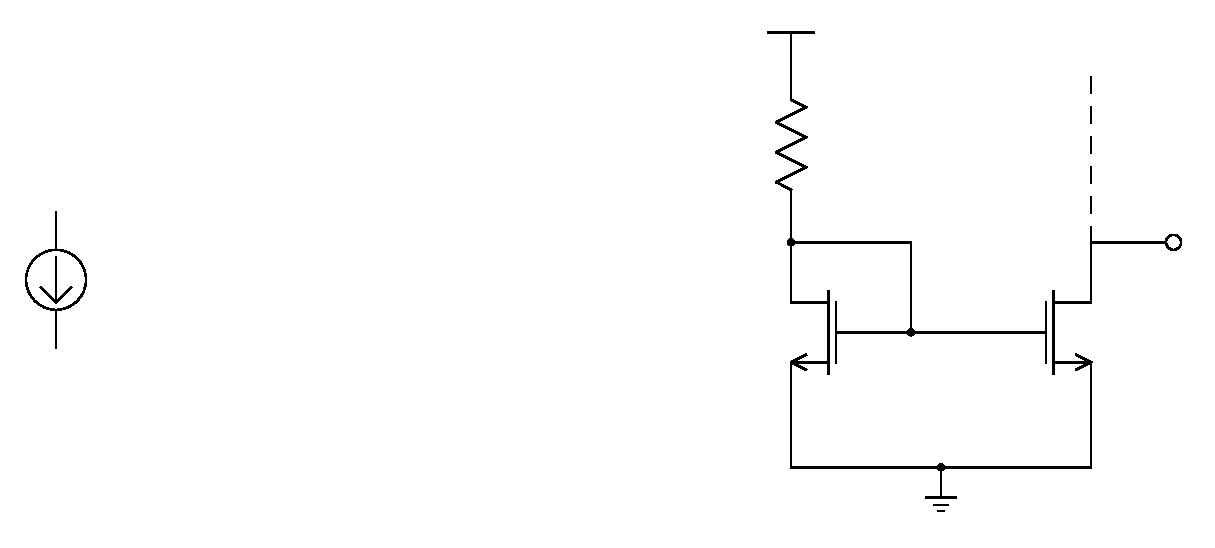
\includegraphics[scale=0.90]{nMosfetConstantCurrentSource}
\caption{منبع مستقل برقی رو}
\label{شکل_ماسفیٹ_پیداکار_مستقل_برقی_رو}
\end{figure}

\اصطلاح {منبع مستقل برقی رو} میں مزاحمت \عددی{R_{\textrm{حوالہ}}} کی مدد سے درکار برقی رو حاصل کیا جاتا ہے۔اس مزاحمت کو تبدیل کرنے سے \عددی{V_{GS1}} اور \عددی{V_{GS2}} تبدیل ہوتے ہیں۔آپ دیکھ سکتے ہیں کہ \عددی{Q_2}  کو \عددی{Q_1} قابو کرتا ہے۔یوں \عددی{Q_2} تابع ماسفیٹ ہے۔مخلوط دور میں دونوں ماسفیٹ کے \عددی{k_n'} اور \عددی{V_t} یکساں ہوتے ہیں۔یوں \عددی{\left(\frac{W}{L} \right)_2} اور \عددی{\left(\frac{W}{L} \right)_1} کی شرح سے  \عددی{I_{\textrm{عکس}}} اور \عددی{I_{\textrm{حوالہ}}} کی شرح تعین ہوتی ہے۔

مندرجہ بالا تبصرے میں \اصطلاح {ارلی برقی دباو} کے اثر کو نظرانداز کرتے ہوئے تصور کیا گیا کہ دو ماسفیٹ کے \عددی{V_{GS}} برابر ہونے کی صورت میں ان کے \عددی{I_{DS}} بھی برابر ہوتے ہیں۔حقیقت میں ایسا نہیں ہوتا اور دو ماسفیٹ جن کے \عددی{V_{GS}} برابر ہوں کے برقی رو صرف اور صرف اسی وقت برابر ہوتے ہیں جب ان کے \عددی{V_{DS}} بھی برابر ہوں۔شکل \حوالہ{شکل_ماسفیٹ_بار_کا_خط} میں ماسفیٹ \عددی{Q_2} کے خط دکھائے گئے ہیں۔\عددی{V_{GS2}} کی قیمت \عددی{V_{GS1}} کے برابر ہے جو قطعی مقدار ہے لہٰذا ان تمام خطوط میں صرف ایک ہی خط کارآمد ہے۔اس خط کو موٹا کر کے دکھایا گیا ہے۔آپ دیکھ سکتے ہیں کہ \عددی{V_{GS}} تبدیل کئے بغیر \عددی{V_{DS}} کے بڑھانے سے \عددی{I_{DS}} بڑھتی ہے۔\عددی{V_{DS2}} کے تبدیلی سے \عددی{I_{\textrm{عکس}}} میں تبدیلی کو ماسفیٹ کے خارجی مزاحمت \عددی{r_o} کی مدد سے حاصل کیا جا سکتا ہے۔
\begin{figure}
\centering
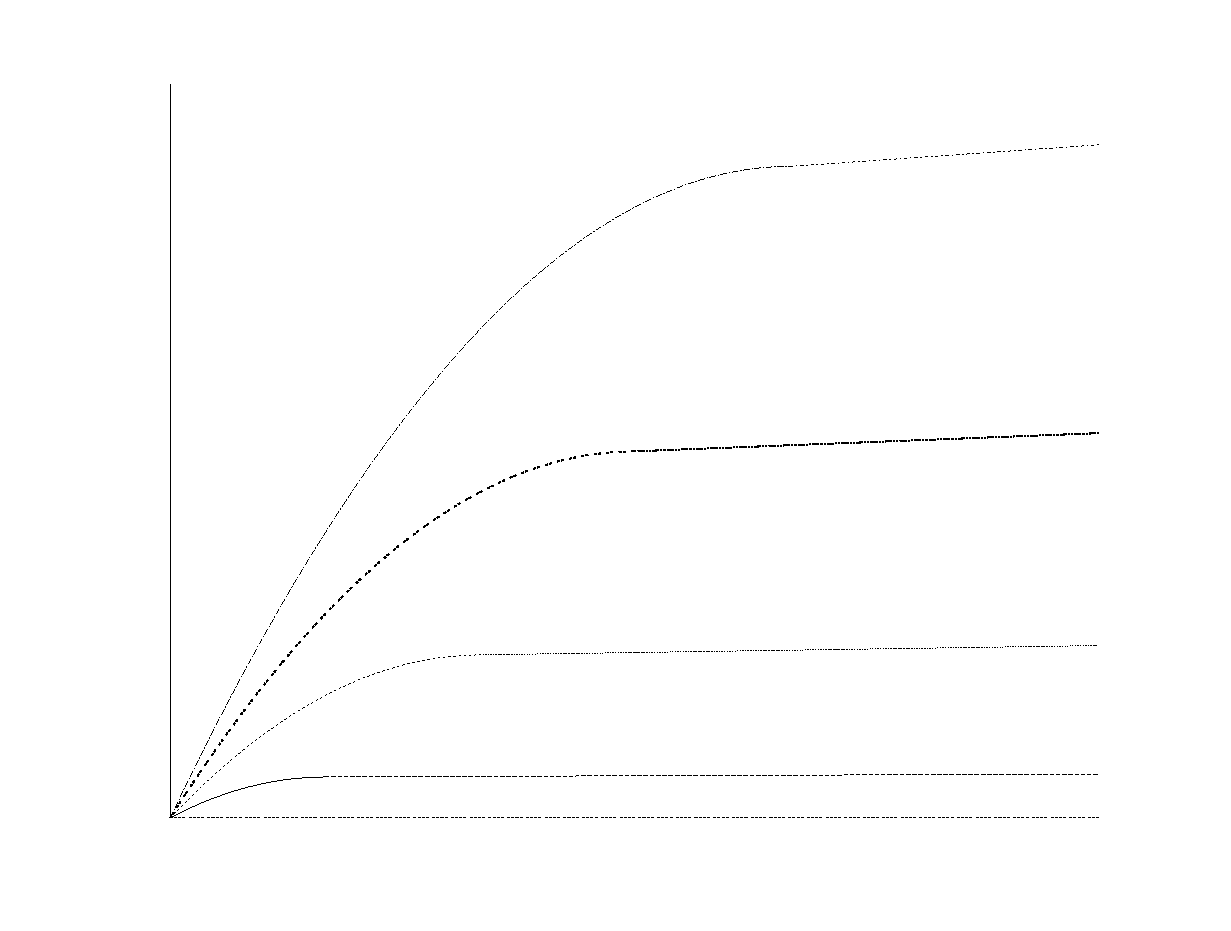
\includegraphics[scale=0.90]{nMosfetCurrentMirrorAsLoad}
\caption{ماسفیٹ کا خط}
\label{شکل_ماسفیٹ_بار_کا_خط}
\end{figure}
%
\begin{figure}
\centering
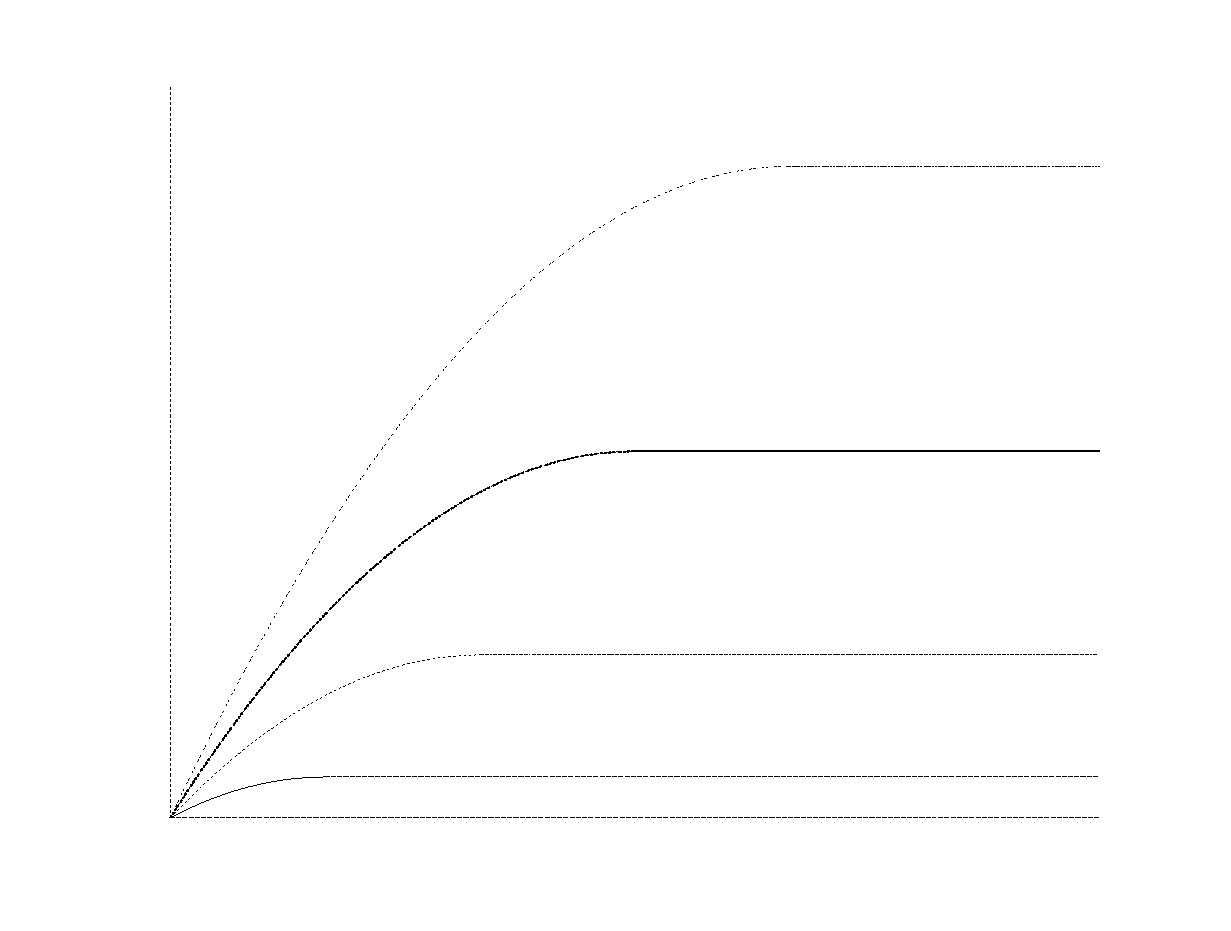
\includegraphics[scale=0.90]{nMosfetCurrentMirror}
\caption{آئینہ برقی رو}
\label{شکل_ماسفیٹ_آئینہ_برقی_رو}
\end{figure}

شکل \حوالہ{شکل_ماسفیٹ_آئینہ_برقی_رو} الف میں \عددی{R_{\textrm{حوالہ}}} کی جگہ دوسرا \اصطلاح {منبع مستقل برقی رو} کا استعمال کیا گیا ہے۔\عددیء{Q_1} میں \عددیء{I_{\textrm{حوالہ}}} برقی رو پائی جاتی ہے۔افزائندہ ماسفیٹ کی مساوات سے  \عددیء{Q_1} کی \عددیء{V_{GS}} حاصل کی جا سکتی ہے جو \عددیء{Q_2} پر بھی لاگو ہے۔یوں آپ دیکھ سکتے ہیں کہ اس صورت میں بھی
\begin{align*}
I_{\textrm{عکس}}=I_{\textrm{حوالہ}}
\end{align*}
ہو گا۔اس شکل میں مثبت برقی منبع کو \عددی{V_{+}} اور منفی کو \عددی{V_{-}} لکھا گیا ہے۔شکل  ب میں \تحریر{pMOSFET} استعمال کرتے ہوئے \اصطلاح {آئینہ برقی رو} بنایا گیا ہے جس کی کارکردگی بالکل \تحریر{nMOSFET} سے بنائے گئے \اصطلاح {آئینہ برقی رو} کی طرح ہے۔فرق صرف اتنا ہے کہ \تحریر{nMOSFET} میں \عددی{I_{\textrm{عکس}}} کی سمت \اصطلاح {آئینہ} کے جانب ہے جبکہ \تحریر{pMOSFET} \اصطلاح {آئینہ} میں \عددی{I_{\textrm{عکس}}} کی سمت \اصطلاح {آئینہ}  سے باہر کو ہے۔    
%==================
\ابتدا{مثال}
\اصطلاح {منبع مستقل برقی رو} میں
\begin{align*}
V_{DD}=\SI{15}{\volt}, \hspace{5mm} k_n=\SI[per=frac,fraction=nice]{0.12}{\milli \ampere \per \volt \squared}, \hspace{5mm} V_t=\SI{2.1}{\volt}
\end{align*}
ہیں۔\عددی{I_{\textrm{عکس}}=\SI{2}{\milli \ampere}} حاصل کرنے کے لئے درکار \عددی{R_{\textrm{حوالہ}}} حاصل کریں۔

حل:\عددی{I_{\textrm{عکس}}=I_{\textrm{حوالہ}}} لیتے ہوئے مساوات \حوالہ{مساوات_ماسفیٹ_مستقل_برقی_رو_الف}
\begin{align*}
2 \times 10^{-3}=\frac{0.12 \times 10^{-3}}{2} \left(V_{GS1}-2.1 \right)^2
\end{align*}
سے
\begin{align*}
V_{GS1}=\SI{7.8735}{\volt}, \hspace{3mm} \SI{-3.67}{\volt}
\end{align*}
 حاصل ہوتے ہیں۔منفی جواب کو رد کیا جاتا ہے چونکہ یہ \عددی{V_t} سے کم ہے جس سے ماسفیٹ منقطع حالت میں ہو گا۔مثبت جواب کو لیتے ہوئے مساوات \حوالہ{مساوات_ماسفیٹ_مستقل_برقی_رو_الف} کو استعمال کرتے ہوئے
\begin{align*}
2 \times 10^{-3}=\frac{15-7.8735}{R_{\textrm{حوالہ}}}
\end{align*}
سے \عددی{R_{\textrm{حوالہ}}=\SI{5.66}{\kilo \ohm}} حاصل ہوتا ہے۔
\انتہا{مثال}

%====================
\ابتدا{مثال}\شناخت{مثال_ماسفیٹ_مستقل_برقی_رو_الف}
شکل \حوالہ{شکل_ماسفیٹ_پیداکار_مستقل_برقی_رو_استعمال} میں دونوں ماسفیٹ کے \عددیء{k_n=\SI{0.2}{\milli \ampere \per \volt \squared}} اور \عددیء{V_t=\SI{1.7}{\volt}} ہیں۔مزید یہ کہ \عددی{R_{\textrm{حوالہ}}=\SI{6.8}{\kilo \ohm}} اور \عددی{R_{\textrm{بوجھ} }=\SI{4.7}{\kilo \ohm}} ہیں۔\عددی{I_{\textrm{عکس}}} اور \عددی{V_O} حاصل کریں۔

\begin{figure}
\centering
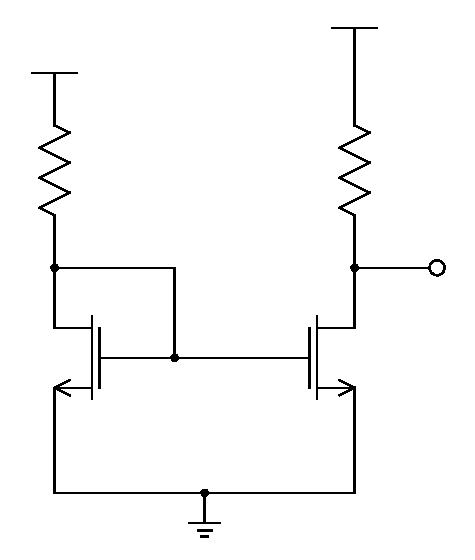
\includegraphics[scale=0.90]{nMosfetConstantCurrentSourceExampleA}
\caption{منبع مستقل برقی رو کی مثال}
\label{شکل_ماسفیٹ_پیداکار_مستقل_برقی_رو_استعمال}
\end{figure}

حل:\عددی{V_{DS1}=V_{GS1}} لیتے ہوئے
\begin{align*}
\frac{12-V_{GS1}}{6800}=\frac{0.2 \times 10^{-3}}{2} \left(V_{GS1}-1.7 \right)^2
\end{align*}
سے
\begin{align*}
V_{GS1}=\SI{4.926}{\volt}, \hspace{3mm} \SI{-2.99}{\volt}
\end{align*}
 حاصل ہوتا ہے۔\عددی{\SI{-2.99}{\volt}} کو رد کیا جاتا ہے چونکہ اس طرح \عددی{V_{GS1} < V_t} حاصل ہوتا ہے جو منقطع ماسفیٹ کو ظاہر کرتا ہے۔مساوات \حوالہ{مساوات_ماسفیٹ_مستقل_برقی_رو_الف} اور \حوالہ{مساوات_ماسفیٹ_مستقل_برقی_رو_ب} دونوں استعمال کرتے ہوئے \عددی{V_{GS1}=\SI{4.926}{\volt}} پر برقی رو حاصل کرتے ہیں۔ظاہر ہے دونوں جوابات برابر ہوں گے۔
\begin{align*}
I_{DS1}&=\frac{12-4.926}{6800}=\SI{1.04}{\milli \ampere}\\
I_{DS1}&=\frac{0.2 \times 10^{-3}}{2} \left(4.926-1.7 \right)^2=\SI{1.04}{\milli \ampere}
\end{align*}
چونکہ یہ \اصطلاح {آئینہ برقی رو} ہے لہٰذا
\begin{align*}
I_{\textrm{عکس}}=I_{\textrm{حوالہ}}=\SI{1.04}{\milli \ampere}
\end{align*}
ہو گا۔\عددی{Q_2} کے ڈرین پر
\begin{align*}
V_O=V_{DS2}&=17-I_{DS2} R_{\textrm{بوجھ} }\\
&=17- 1.04 \times 10^{-3} \times 4700\\
&=\SI{12.1}{\volt}
\end{align*}
ہیں۔یوں \عددی{Q_2} کا 
\begin{align*}
V_{GD2}=V_{GS2}-V_{DS2}=4.925-12.1=\SI{-7.1}{\volt}
\end{align*}
حاصل ہوتا ہے۔چونکہ \عددی{V_{GD2} < V_t} ہے لہٰذا \عددی{Q_2} افزائندہ خطے میں ہی ہے۔
\انتہا{مثال}
%===============
\ابتدا{مثال}
مندرجہ بالا مثال میں \عددی{R_{\textrm{بوجھ} }} کی وہ قیمت حاصل کریں جس پر \عددی{Q_2} افزائندہ خطے سے نکل آئے گا۔

حل:\عددی{Q_2} اس وقت تک افزائندہ رہے گا جب تک \عددی{V_{GD2} < Vt} ہو۔چونکہ \عددی{V_{GS2}=V_{GS1}=\SI{4.925}{\volt}} ہی رہے گا جبکہ
\begin{align*}
V_{DS2}&=17-I_{DS2} R_{\textrm{بوجھ} }\\
&=17-1.04 \times 10^{-3} \times R_{\textrm{بوجھ} }
\end{align*}
کے برابر ہے۔یوں \عددی{Q_2} اس وقت افزائندہ خطے سے باہر نکلے گا جب 
\begin{align*}
V_{GD2}&=V_{GS2}-V_{DS2}> V_t\\
&=4.925-\left(17-1.04 \times 10^{-3} \times R_{\textrm{بوجھ} } \right) > 1.7
\end{align*} 
ہو گا۔یوں  تقریباً \عددی{R_{\textrm{بوجھ} }> \SI{13.24}{\kilo \ohm}} حاصل ہوتا ہے۔مثال کے طور پر اگر بوجھ کی مزاحمت \عددی{\SI{15}{\kilo \ohm}}
کر دیا جائے تب \عددی{V_{DS2}=\SI{1.4}{\volt}} اور \عددی{V_{GD2}=\SI{3.5}{\volt}} حاصل ہوتا ہے جو کہ \عددی{V_t} سے زیادہ ہے یعنی ماسفیٹ افزائندہ خطے میں نہیں ہے۔
\انتہا{مثال}
%===========================
\ابتدا{مثال}
مثال \حوالہ{مثال_ماسفیٹ_مستقل_برقی_رو_الف} میں \عددیء{V_{DS1}=\SI{4.926}{\volt}}، \عددیء{V_{DS2}=\SI{12.1}{\volt}} اور \عددی{I_{\textrm{عکس}}=\SI{1.04}{\milli \ampere}} حاصل ہوئے۔ \عددی{V_A=\SI{50}{\volt}} کی صورت میں \عددی{I_{\textrm{عکس}}} حاصل کردہ قیمت سے کتنا انحراف کرے گا۔

حل: ماسفیٹ کا خارجی مزاحمت تقریباً
\begin{align*}
r_o=\frac{50}{1.04 \times 10^{-3}} \approx \SI{48}{\kilo \ohm}
\end{align*} 
ہے۔اگر \عددی{V_{DS2}} کی قیمت \عددی{\SI{4.926}{\volt}} ہوتا تب تو \عددی{I_{DS2}} بھی \عددی{\SI{1.04}{\milli \ampere}} ہوتا۔البتہ \عددی{V_{DS2}} 
\begin{align*}
12.1-4.926=\SI{7.175}{\volt}
\end{align*}
زیادہ ہے لہٰذا ماسفیٹ کے خارجی مزاحمت کی تعریف
\begin{align*}
r_o=\frac{\Delta V_{DS}}{\Delta I_{DS}}
\end{align*}
سے
\begin{align*}
\Delta I_{DS}=\frac{7.175}{48000} \approx \SI{149}{\micro \ampere}
\end{align*}
ہو گا۔یوں
\begin{align*}
 I_{\textrm{حوالہ}}=\SI{1.04}{\milli \ampere}+\SI{149}{\micro \ampere}=\SI{1.189}{\milli \ampere}
\end{align*}
ہو گا۔
\انتہا{مثال}
%============

\حصہ{مزاحمت کے عکس}
دو جوڑ ٹرانزسٹر کے حصہ \حوالہ{حصہ_ٹرانزسٹر_مزاحمت_کا_عکس} میں آپ نے دیکھا کہ ٹرانزسٹر کے ایمٹر پر پائے جانے والے بیرونی مزاحمت \عددی{R_E} کا ٹرانزسٹر کے بیس جانب عکس \عددی{\left(\beta+1 \right) R_E} نظر آتا ہے۔اسی طرح ٹرانزسٹر کے ایمٹر پر اس کے اندرونی مزاحمت \عددی{r_e} کا عکس ٹرانزسٹر کے بیس جانب \عددی{\left(\beta+1 \right) r_e} نظر آتا ہے جسے \عددی{r_{be}} لکھا جاتا ہے۔ٹرانزسٹر کے بیس جانب بیرونی جڑے مزاحمت \عددی{R_B} کا عکس ٹرانزسٹر کے ایمٹر جانب \عددی{\tfrac{R_B}{\beta+1}} نظر آتا ہے۔اسی طرح ٹرانزسٹر کے بیس جانب ٹرانزسٹر کی اندرونی مزاحمت \عددی{r_{be}} کا عکس ٹرانزسٹر کے ایمٹر  جانب \عددی{\tfrac{r_{be}}{\beta+1}} نظر آتا ہے جسے \عددی{r_e} لکھا جاتا ہے۔برقی دباو کا عکس بیس سے ایمٹر یا ایمٹر سے بیس جانب تبدیلی کے بغیر جوں کا توں نظر آتا ہے۔
\begin{figure}
\centering
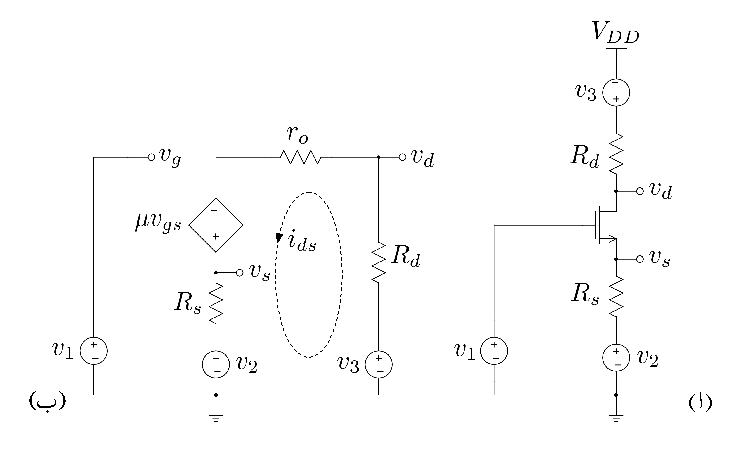
\includegraphics[scale=0.90]{mosfetResistanceMirrorA}
\caption{مزاحمت کے عکس}
\label{شکل_ماسفیٹ_مزاحمت_کے_عکس}
\end{figure}

ماسفیٹ میں مزاحمت کے عکس پر گفتگو کرنے کی خاطر شکل \حوالہ{شکل_ماسفیٹ_مزاحمت_کے_عکس} الف پر غور کرتے ہیں۔اس دور میں ماسفیٹ کے تینوں سروں پر اشارات فراہم کئے گئے ہیں تا کہ مختلف ممکنات کو دیکھا جا سکے۔ماسفیٹ مائل کرنے والے اجزاء کو شامل نہیں کیا گیا ہے تا کہ اصل موضوع پر توجہ رہے۔

شکل  ب میں اس کا باریک اشاراتی مساوی دور دکھایا گیا ہے جسے دیکھتے ہوئے
\begin{align*}
i_{ds}=\frac{\mu v_{gs}+v_3-v_2}{R_s+r_o+R_d}
\end{align*}
لکھا جا سکتا ہے جہاں
\begin{align*}
v_{gs}=v_1-i_{ds} R_s-v_2
\end{align*}
کے برابر ہے۔ان دو مساوات کو ملا کر حاصل ہوتا ہے
\begin{align}\label{مساوات_ماسفیٹ_محاصل_عکس}
i_{ds}=\frac{\mu v_1+v_3-\left(\mu+1 \right) v_2}{\left(\mu+1 \right) R_s+r_o+R_d}
\end{align}

مساوات \حوالہ{مساوات_ماسفیٹ_محاصل_عکس} سے شکل \حوالہ{شکل_ماسفیٹ_مزاحمت_کے_عکس_ب} حاصل ہوتا ہے۔اس شکل کو دیکھتے ہوئے یہ حقیقت سامنے آتی ہے کہ ڈرین پر پائے جانے والے  \عددیء{v_3}، \عددی{r_o} اور \عددی{R_d} جوں کے توں ہیں جبکہ سورس پر پائے جانے والے \عددیء{v_1} اور \عددیء{R_s} دونوں  \عددی{\left(\mu+1 \right)} سے ضرب شدہ ہیں جبکہ گیٹ پر پائے جانے والا \عددی{v_1} صرف \عددی{\mu} سے ضرب شدہ ہے۔ڈرین پر پائے جانے والے اجزاء جوں کے توں ہیں لہٰذا یہ شکل ڈرین سے دیکھتے ہوئے نظر آئے گی۔اس طرح ڈرین سے دیکھتے ہوئے سورس پر پائے جانے والا مزاحمت اور برقی اشارہ دونوں  کا عکس \عددی{\left(\mu+1 \right)} سے ضرب ہوتا نظر آئے گا جبکہ  گیٹ پر برقی اشارہ صرف \عددی{\mu} سے ضرب ہوتا نظر آئے گا۔ 
%
\begin{figure}
\centering
\includegraphics[scale=0.90]{mosfetResistanceMirrorB}
\caption{ڈرین جانب عکس}
\label{شکل_ماسفیٹ_مزاحمت_کے_عکس_ب}
\end{figure}

مساوات \حوالہ{مساوات_ماسفیٹ_محاصل_عکس} کے  کسر میں اوپر اور نچلے دونوں حصوں کو \عددی{\mu+1} سے تقسیم کرتے ہوئے یوں لکھا جا سکتا ہے
\begin{align}\label{مساوات_ماسفیٹ_محاصل_عکس_الف}
i_{ds}=\frac{\frac{\mu v_1}{\mu+1}+\frac{v_3}{\mu+1}- v_2}{R_s+\frac{r_o}{\mu+1}+\frac{R_d}{\mu+1}}
\end{align}
جس سے شکل \حوالہ{شکل_ماسفیٹ_مزاحمت_کے_عکس_پ} حاصل ہوتا ہے۔یہاں آپ دیکھ سکتے ہیں کہ سورس کا مزاحمت \عددی{R_s} اور اشارہ \عددی{v_2} جوں کے توں ہیں جبکہ ڈرین اور گیٹ کے اشارات اور مزاحمت کے عکس نظر آتے ہیں۔اس طرح سورس سے دیکھتے ہوئے ڈرین کے اجزاء یعنی \عددیء{v_3}، \عددیء{R_d} اور \عددی{r_o} تینوں \عددی{\left(\mu+1 \right)} سے تقسیم ہوتے نظر آتے ہیں۔جیسے گزشتہ شکل میں دیکھا گیا تھا کہ \عددی{v_1} کا عکس ڈرین پر \عددی{\mu} سے ضرب ہوتا نظر آتا ہے اور ڈرین پر پائے جانے والے اس عکس کا سورس جانب عکس \عددی{\left (\mu+1 \right)}سے تقسیم ہوتا ہے۔
%
\begin{figure}
\centering
\includegraphics[scale=0.90]{mosfetResistanceMirrorC}
\caption{سورس جانب عکس}
\label{شکل_ماسفیٹ_مزاحمت_کے_عکس_پ}
\end{figure}
%=============
\حصہ{تابع سورس (ڈرین مشترک ایمپلیفائر)}
\جزوحصہء{نقطہ  مائل}
شکل \حوالہ{شکل_ماسفیٹ_تابع_مخارج} الف میں \اصطلاح {گھٹاتا ماسفیٹ} کا \اصطلاح {تابع سورس} ایمپلیفائر دکھایا گیا ہے۔یہاں \عددی{nFET} بھی استعمال کیا جا سکتا تھا۔ایسا دور منفی \عددی{V_{GSQ}} مہیا کرنے کی خاطر استعمال کیا جاتا ہے۔\اصطلاح {یک سمتی رو خطِ بوجھ} لکھتے ہیں۔
\begin{align}\label{مساوات_ماسفیت_تابع_مخارج_بار_کا_خط}
V_{DD}&=v_{DS}+i_{DS} \left(R_1+R_2 \right)
\end{align}
نقطہ  مائل یک سمتی مقداروں سے حاصل ہوتا ہے۔مزاحمت \عددی{R_g} میں صفر یک سمتی برقی رو ہونے کی وجہ سے اس کے دونوں سروں پر برابر یک سمتی برقی دباو پایا جائے گا۔شکل  الف میں \عددی{R_g} کے نچلے سرے پر \عددی{I_{DSQ}R_2} برقی دباو پایا جاتا ہے اور یوں ماسفیٹ کے گیٹ پر بھی یہی برقی دباو ہو گا۔ماسفیٹ کے سورس پر \عددی{I_{DSQ} \left(R_1+R_2 \right)} برقی دباو ہے۔یوں ماسفیٹ کے لئے ہم لکھ سکتے ہیں
\begin{gather}
\begin{aligned}\label{مساوات_ماسفیت_تابع_مخارج_نقطہ _مائل}
V_{GSQ}&=V_{GQ}-V_{SQ}\\
&=I_{DSQ} \left( R_2\right)-I_{DSQ} \left(R_1+R_2 \right)\\
&=-I_{DSQ} R_1
\end{aligned}
\end{gather}
عموماً \عددی{V_{GSQ}} چند وولٹ کے برابر ہو گا جبکہ \عددی{V_{DSQ}} تقریباً \عددی{V_{DD}} کے نصف کے برابر ہو گا۔یوں کسی بھی حقیقی ایمپلیفائر میں \عددی{R_1 \ll R_2} ہو گا۔
%
\begin{figure}
\centering
\includegraphics[scale=0.90]{mosfetSourceFollower}
\caption{تابع سورس}
\label{شکل_ماسفیٹ_تابع_مخارج}
\end{figure}
\جزوحصہء{افزائش \عددی{A_v}}
شکل \حوالہ{شکل_ماسفیٹ_تابع_مخارج} ب میں باریک اشاراتی مساوی دور بنانے کی غرض سے \عددی{V_{DD}} اور گیٹ کپیسٹر کو قصر دور کیا گیا ہے۔مزید گیٹ اور سورس کو علیحدہ کرنے کی خاطر \عددی{v_i} کو دو مرتبہ بنایا گیا ہے جہاں نقطہ دار لکیر کے دونوں سروں پر ہر وقت برابر برقی اشارہ \عددی{v_i} پایا جاتا ہے۔نقطہ  دار لکیر کو مٹانے سے گیٹ اور سورس دونوں جانب کوئی تبدیلی نہیں پیدا ہوتی چونکہ دونوں جانب \عددی{v_i} اپنی جگہ پر برقرار پایا جاتا ہے۔یوں شکل \حوالہ{شکل_ماسفیٹ_مزاحمت_کے_عکس_پ} کے طرز پر باریک اشاراتی مساوی دور بناتے ہوئے شکل \حوالہ{شکل_ماسفیٹ_تابع_مخارج_مساوی} الف حاصل ہوتا ہے۔اس شکل میں تمام اجزاء کو سورس منتقل کیا گیا ہے۔\عددیء{R_2}، \عددیء{R_g} اور \عددی{v_i} کی جگہ ان کا تھونن مساوی دور استعمال کرتے ہوئے شکل \حوالہ{شکل_ماسفیٹ_تابع_مخارج_مساوی} ب حاصل ہوتا ہے جہاں
\begin{align*}
v_{th}&=\frac{R_2 v_i}{R_2+R_g}\\
R_{th}&=\frac{R_2 R_g}{R_2+R_g}=R_2 \mathbin{\|} R_g
\end{align*}
کے برابر ہیں۔شکل \حوالہ{شکل_ماسفیٹ_تابع_مخارج_مساوی} ب میں
\begin{align*}
R_s=R_1+\left(R_2 \mathbin{\|} R_g \right)
\end{align*}
لکھتے ہوئے
\begin{gather}
\begin{aligned}\label{مساوات_ماسفیٹ_تابع_مشترک_الف}
i_{ds}&=\frac{\left[\frac{\mu}{\mu+1}-\frac{R_2}{R_2+R_g}\right]v_i}{\frac{r_o}{\mu+1}+R_s}\\
v_L&=i_{ds} R_s+\frac{R_2}{R_2+R_g}v_i
\end{aligned}
\end{gather}
لکھا جا سکتا ہے جس سے
\begin{align*}
v_L=\left[\frac{\frac{\mu}{\mu+1}-\frac{R_2}{R_2+R_g}}{\frac{r_o}{\mu+1}+R_s}\right] R_s v_i+\frac{R_2}{R_2+R_g}v_i
\end{align*}
حاصل ہوتا ہے ۔جس سے \عددی{A_v=\tfrac{v_L}{v_i}} یوں حاصل ہوتا ہے۔
\begin{align}\label{مساوات_ماسفیٹ_تابع_مخارج_افزائش_الف}
A_v=\frac{\left(\frac{\mu}{\mu+1}\right) R_s +\left(\frac{R_2}{R_2+R_g}\right)\left( \frac{r_o}{\mu+1} \right)}{\frac{r_o}{\mu+1}+R_s}
\end{align}
چونکہ \عددی{\mu=g_m r_o} کے برابر ہے لہٰذا \عددی{\tfrac{r_o}{\mu+1} \approx \tfrac{1}{g_m}} لکھا جا سکتا ہے جس سے  مندرجہ بالا مساوات کو یوں بھی لکھ سکتے ہیں۔
\begin{align}\label{مساوات_ماسفیٹ_تابع_مخارج_افزائش_ب}
A_v=\frac{g_m \left(\frac{\mu}{\mu+1}\right) R_s +\left(\frac{R_2}{R_2+R_g}\right)}{1+g_m R_s}
\end{align}
اگر \عددی{R_g \gg R_2} ہو، جیسا کہ عموماً ہوتا ہے، تب \عددی{\tfrac{R_2}{R_2+R_g}} کو نظر انداز کرتے ہوئے اس مساوات کو یوں لکھا جا سکتا ہے۔
\begin{align}\label{مساوات_ماسفیٹ_تابع_مخارج_افزائش_پ}
A_v \approx \frac{g_m \left(\frac{\mu}{\mu+1}\right) R_s}{1+g_m R_s}
\end{align}
عموماً \عددی{R_g \gg R_2} اور یوں \عددی{R_s \approx R_1+R_2} لکھا جا سکتا ہے۔اگر \عددی{g_m R_s\gg1} بھی ہو تب مندرجہ بالا مساوات کو
\begin{align}\label{مساوات_ماسفیٹ_تابع_مخارج_افزائش_ت}
A_v \approx \frac{\mu}{\mu+1} \approx 1
\end{align}
لکھا جا سکتا ہے۔اس مساوات سے صاف ظاہر ہے کہ ماسفیٹ کے \اصطلاح {تابع سورس ایمپلیفائر} کا خارجی اشارہ بھی خوش اسلوبی سے داخلی اشارے کی پیروی کرتا ہے۔دو جوڑ ٹرانزسٹر کی طرح ماسفیٹ کے مشترکہ ڈرین ایمپلیفائر کا \عددی{A_v} بھی تقریباً ایک کے برابر ہے۔
% 
\begin{figure}
\centering
\includegraphics[scale=0.90]{mosfetSourceFollowerEquivalent}
\caption{تابع سورس کا مساوی باریک اشاراتی دور}
\label{شکل_ماسفیٹ_تابع_مخارج_مساوی}
\end{figure}

\جزوحصہء{خارجی مزاحمت}
شکل \حوالہ{شکل_ماسفیٹ_تابع_مخارج_مساوی} ب کو دیکھتے ہوئے خارجی مزاحمت یوں لکھی جا سکتی ہے۔
\begin{gather}
\begin{aligned}
R_o&=\frac{r_o}{\mu+1} \mathbin{\|} R_s \\
&=\frac{1}{g_m} \mathbin{\|} R_s
\end{aligned}
\end{gather}
اگر \عددی{R_s \gg \tfrac{1}{g_m}} ہو تب اسے یوں لکھا جا سکتا ہے۔
\begin{align}
R_o \approx \frac{1}{g_m}
\end{align}

\جزوحصہء{داخلی مزاحمت}
داخلی مزاحمت شکل \حوالہ{شکل_ماسفیٹ_تابع_مخارج} الف میں \عددی{\tfrac{v_i}{i_i}} سے حاصل ہو گی۔چونکہ گیٹ کی برقی رو صفر ہوتی ہے لہٰذا \عددی{i_i} وہ برقی رو ہے جو مزاحمت \عددی{R_g} سے گزرتی ہے۔شکل \حوالہ{شکل_ماسفیٹ_تابع_مخارج} ب میں اس کی نشاندہی کی گئی ہے۔چونکہ اس شکل میں \عددی{v_i} دو جگہ نظر آتا ہے لہٰذا یہ ضروری ہے کہ \عددی{R_g} کے ساتھ جڑی \عددی{v_i} پر نظر رکھی جائے۔
\begin{figure}
\centering
\includegraphics[scale=0.90]{mosfetSourceFollowerEquivalentInputImpedance}
\caption{تابع سورس کا داخلی مزاحمت}
\label{شکل_ماسفیٹ_تابع_مخارج_داخلی_مزاحمت}
\end{figure}

شکل \حوالہ{شکل_ماسفیٹ_تابع_مخارج_مساوی} الف کو قدر مختلف طرز پر  شکل \حوالہ{شکل_ماسفیٹ_تابع_مخارج_داخلی_مزاحمت} الف میں دکھایا گیا ہے جہاں مطلوبہ \عددی{v_i} اور \عددی{i_i} کی وضاحت کی گئی ہے۔\عددی{R_g} کے بائیں جانب کا \اصطلاح {تھونن مساوی} دور لیتے ہوئے
\begin{gather}
\begin{aligned}
v_{th}&=\frac{R_2 \left(\frac{\mu }{\mu+1} \right) v_i}{R_1+R_2+\frac{r_o}{\mu+1}}\\
R_{th}&=R_2 \mathbin{\|} \left(\frac{r_o}{\mu+1}+R_1 \right)
\end{aligned}
\end{gather}
حاصل ہوتا ہے۔شکل \حوالہ{شکل_ماسفیٹ_تابع_مخارج_داخلی_مزاحمت} ب میں حاصل کردہ تھونن دور استعمال کیا گیا ہے۔یوں
\begin{align*}
i_i&=\frac{v_i-v_{th}}{R_g+R_{th}}\\
&=\frac{v_i-\frac{R_2 \left(\frac{\mu }{\mu+1} \right) v_i}{R_1+R_2+\frac{r_o}{\mu+1}}}{R_g+R_2 \mathbin{\|} \left(\frac{r_o}{\mu+1}+R_1 \right)}
\end{align*}
لکھتے ہوئے داخلی مزاحمت \عددی{R_i} یوں حاصل ہوتا ہے۔
\begin{align}\label{مساوات_ماسفیٹ_تابع_مخارج_داخلی_مزاحمت_الف}
R_i=\frac{v_i}{i_i}=\frac{R_g+R_2 \mathbin{\|} \left(\frac{r_o}{\mu+1}+R_1 \right)}{1-\frac{R_2 \left(\frac{\mu }{\mu+1} \right)}{R_1+R_2+\frac{r_o}{\mu+1}}}
\end{align}
اس مساوات میں \عددی{\tfrac{r_o}{\mu+1} \approx \tfrac{1}{g_m}} پر کرنے سے
\begin{align}\label{مساوات_ماسفیٹ_تابع_مخارج_داخلی_مزاحمت_ب}
R_i=\frac{R_g+R_2 \mathbin{\|} \left(\frac{1}{g_m}+R_1 \right)}{1-\frac{g_m R_2 \left(\frac{\mu }{\mu+1} \right)}{g_m \left(R_1+R_2\right)+1}}
\end{align}
حاصل ہوتا ہے۔اگر \عددی{R_g \gg R_2} اور \عددی{g_m \left(R_1+R_2 \right) \gg 1} ہوں، جیسا کہ عموماً ہوتا ہے، تب اس مساوات کو
\begin{align}\label{مساوات_ماسفیٹ_تابع_مخارج_داخلی_مزاحمت_پ}
R_i \approx \frac{R_g}{1-\frac{R_2 \left(\frac{\mu}{\mu+1} \right)}{R_1+R_2}}
\end{align}
لکھا جا سکتا ہے۔اگر ساتھ ہی ساتھ \عددی{R_2 \gg R_1} ہو تب اس سے مزید سادہ مساوات یوں حاصل ہوتی ہے۔
\begin{align} \label{مساوات_ماسفیٹ_تابع_مخارج_داخلی_مزاحمت_ت}
R_i \approx \left(\mu+1 \right) R_g
\end{align}

مثال \حوالہ{مثال_ٹرانزسٹر_تابع_مخارج_داخلی_مزاحمت_بڑھایا_گیا_ہے} میں  بیس سے ایمٹر مزاحمت جوڑنے سے داخلی مزاحمت میں اضافہ ہوتا دکھایا گیا۔یہاں بھی ایسا کرنے سے داخلی مزاحمت کی قیمت \عددی{R_g} سے زیادہ ہو جاتی ہے۔
%==============
\ابتدا{مثال}
شکل \حوالہ{شکل_ماسفیٹ_تابع_مخارج} الف میں استعمال کئے جانے والے ماسفیٹ کے
 \عددیء{k_n=\SI[per=frac,fraction=nice]{0.2}{\milli \ampere \per \volt \squared}}، \عددیء{V_t=\SI{-3}{\volt}} اور \عددی{r_o=\SI{90}{\kilo \ohm}} ہیں۔\عددی{\SI{15}{\volt}} کی منبع استعمال کرتے ہوئے \عددیء{I_{DSQ}=\SI{0.4}{\milli \ampere}}، \عددی{V_{DSQ}=\SI{10}{\volt}} اور \عددی{R_i=\SI{200}{\kilo \ohm}} حاصل کرنے کی خاطر درکار مزاحمت حاصل کریں۔

حل:
\begin{align*}
I_{DSQ}&=\frac{k_n}{2} \left(V_{GS}-V_t \right)^2\\
0.0004&=\frac{0.0002}{2} \left(V_{GSQ}+3 \right)^2
\end{align*}
سے
\begin{align*}
V_{GSQ}=\SI{-5}{\volt},\hspace{3mm} \SI{-1}{\volt}
\end{align*}
حاصل ہوتے ہیں۔\عددی{V_{GSQ}=\SI{-5}{\volt}} کو رد کیا جاتا ہے چونکہ یہ قیمت \عددی{V_t} سے کم ہے جس سے ماسفیٹ منقطع ہو جاتا ہے۔یوں مساوات \حوالہ{مساوات_ماسفیت_تابع_مخارج_نقطہ _مائل} کے تحت \عددی{R_1=\SI{2.5}{\kilo \ohm}} حاصل ہوتا ہے۔مساوات \حوالہ{مساوات_ماسفیت_تابع_مخارج_بار_کا_خط} کی مدد سے
\begin{align*}
R_1+R_2&=\frac{V_{DD}-V_{DSQ}}{I_{DSQ}}\\
&=\frac{15-10}{0.4 \times 10^{-3}}\\
&=\SI{12.5}{\kilo \ohm}
\end{align*}
حاصل ہوتا ہے اور یوں \عددی{R_2=\SI{10}{\kilo \ohm}} ہو گا۔چونکہ
\begin{align*}
V_{GD}=V_{GS}-V_{DS}=-1-10=\SI{-11}{\volt} < V_t
\end{align*}
ہے لہٰذا ماسفیٹ کو افزائندہ خطے میں ٹھیک تصور کیا گیا تھا۔

مساوات \حوالہ{مساوات_میدانی_موصلیت_نما_الف} سے 
\begin{align*}
g_m=\sqrt{2 k_n I_{DS}}=\sqrt{2 \times 0.2 \times 10^{-3} \times 0.4 \times 10^{-3}}=\SI{0.4}{\milli \siemens}
\end{align*}
اور یوں \عددی{\mu=g_m r_o=36} حاصل ہوتا ہے۔\عددی{R_g \gg R_2} تصور کرتے ہوئے \عددی{R_s \approx R_1+R_2=\SI{12.5}{\kilo \ohm}} حاصل ہوتا ہے اور یوں مساوات \حوالہ{مساوات_ماسفیٹ_تابع_مخارج_افزائش_پ} سے
\begin{align*}
A_v \approx \frac{0.4 \times 10^{-3} \left(\frac{36}{36+1}\right) 12.5 \times 10^{3}}{1+0.4 \times 10^{-3}\times 12.5 \times 10^{3}}=\SI[per=frac,fraction=nice]{0.81}{\volt \per \volt}
\end{align*}
حاصل ہوتا ہے۔

مساوات \حوالہ{مساوات_ماسفیٹ_تابع_مخارج_داخلی_مزاحمت_پ} کی مدد سے \عددی{R_i=\SI{200}{\kilo \ohm}} حاصل کرنے کی خاطر
\begin{align*}
200000 = \frac{R_g}{1-\frac{10000 \left(\frac{36}{36+1} \right)}{2500+10000}}
\end{align*}
سے \عددی{R_g=\SI{44}{\kilo \ohm}} حاصل ہوتا ہے۔
\انتہا{مثال}
 %========================
\حصہ{گیٹ مشترک ایمپلیفائر}
شکل \حوالہ{شکل_ماسفیٹ_قابو_مشترک_ایمپلیفائر} الف میں \اصطلاح {گیٹ مشترک ایمپلیفائر} دکھایا گیا ہے جبکہ شکل  ب میں اسی کا مساوی بدلتی رو دور دکھایا گیا ہے۔گیٹ پر نسب کپیسٹر کی قیمت لامحدود دکھائی گئی ہے۔یوں درکار تعدد پر کپیسٹر کو قصر دور تصور کیا گیا ہے۔شکل  ب کا شکل \حوالہ{شکل_ماسفیٹ_مزاحمت_کے_عکس} کے ساتھ موازنہ کریں۔یہاں \عددی{v_1} اور \عددی{v_3} صفر وولٹ ہیں جبکہ \عددی{v_2} کو \عددی{v_i} کہا گیا ہے۔لہٰذا تمام اجزاء کو ڈرین میں منتقل کرتے ہوئے شکل \حوالہ{شکل_ماسفیٹ_مزاحمت_کے_عکس_ب} کے طرز پر  شکل \حوالہ{شکل_ماسفیٹ_قابو_مشترک_ایمپلیفائر_عکس} الف حاصل ہوتا ہے۔اسی طرح سورس جانب کا عکس شکل  ب میں دکھایا گیا ہے۔ 
\begin{figure}
\centering
\includegraphics[scale=0.90]{mosfetCommonGateAmplifier}
\caption{گیٹ مشترک ایمپلیفائر}
\label{شکل_ماسفیٹ_قابو_مشترک_ایمپلیفائر}
\end{figure}

شکل \حوالہ{شکل_ماسفیٹ_قابو_مشترک_ایمپلیفائر_عکس} الف کو دیکھتے ہوئے ہم لکھ سکتے ہیں
\begin{align*}
v_L=\frac{R_d}{\left(\mu+1 \right) r_i+r_o+R_d} \left(\mu+1 \right) v_i
\end{align*}
جس سے افزائش \عددی{A_v=\tfrac{v_L}{v_i}} یوں لکھی جا سکتی ہے
\begin{align*}
A_v=\frac{\left(\mu+1 \right)R_d}{\left(\mu+1 \right) r_i+r_o+R_d} 
\end{align*}
%
\begin{figure}
\centering
\includegraphics[scale=0.90]{mosfetCommonGateSourceView}
\caption{گیٹ مشترک ایمپلیفائر کے ڈرین اور سورس جانب عکس}
\label{شکل_ماسفیٹ_قابو_مشترک_ایمپلیفائر_عکس}
\end{figure}

شکل \حوالہ{شکل_ماسفیٹ_قابو_مشترک_ایمپلیفائر_عکس} ب سے ایمپلیفائر کا داخلی مزاحمت لکھا جا سکتا ہے یعنی
\begin{align*}
R_i=\frac{r_o+R_d}{\mu+1}
\end{align*}

گیٹ مشترک ایمپلیفائر بلند تعدد پر استعمال ہوتا ہے۔یہ بطور برقی سوئچ بھی استعمال کیا جاتا ہے۔
%=======================
\حصہ{زنجیری ایمپلیفائر}
ایک سے زیادہ ایمپلیفائر کو زنجیر کی شکل میں جوڑ کر زیادہ سے زیادہ افزائش حاصل کرنا ممکن ہوتا ہے۔ایسے زنجیری ایمپلیفائر میں عموماً داخلی جانب پہلی کڑی،  درکار داخلی مزاحمت فراہم کرنے کی غرض سے تخلیق دیا جاتا ہے جبکہ آخری کڑی کو درکار خارجی مزاحمت کے لئے تخلیق دیا جاتا ہے۔درمیانی کڑیاں درکار افزائش حاصل کرنے کے لئے تخلیق دیں جاتی ہیں۔
 
\ابتدا{مثال}\شناخت{مثال_ماسفیٹ_دو_کڑی_زنجیر}
شکل \حوالہ{شکل_ماسفیٹ_دو_کڑی_زنجیری_الف} میں دو بالکل یکساں ماسفیٹ استعمال کرتے ہوئے، پہلی کڑی سورس مشترک اور دوسری کڑی ڈرین مشترک ایمپلیفائر سے تخلیق دی گئی ہے۔\عددی{k_n=\SI{0.6}{\milli \ampere \per \volt \squared}} اور \عددی{V_t=\SI{1}{\volt}} ہیں۔\عددی{I_{DS1}=\SI{0.12}{\milli \ampere}}، \عددی{I_{DS2}=\SI{1.2}{\milli \ampere}} اور \عددی{V_{DS1}=V_{DS2}=\SI{5}{\volt}} حاصل کرنے کے لئے درکار \عددی{R_{D1}}، \عددی{R_{S1}} اور \عددی{R_{S2}} حاصل کریں۔\عددی{R_{\textrm{داخلی}}=\SI{150}{\kilo \ohm}} حاصل کرنے کے لئے درکار \عددی{R_1} اور \عددی{R_2} حاصل کریں۔تمام کپیسٹروں کی قیمت لامحدود تصور کریں۔

\begin{figure}
\centering
\includegraphics[scale=0.90]{nMosfetCascadedCommonSourceCommonDrain}
\caption{دو کڑی زنجیری ماسفیٹ ایمپلیفائر}
\label{شکل_ماسفیٹ_دو_کڑی_زنجیری_الف}
\end{figure}

حل:\عددی{Q_2} کے خارجی جانب کرچاف کے قانون برائے برقی دباو سے
\begin{align*}
9+5 &=V_{DS2}+I_{DS2}R_{S2}\\
&=5+1.2 \times 10^{-3} R_{S2}
\end{align*}
سے \عددی{R_{S2}=\SI{7.5}{\kilo \ohm}} حاصل ہوتا ہے۔افزائندہ ماسفیٹ کی مساوات سے 
\begin{align*}
1.2 \times 10^{-3}&=\frac{0.6 \times 10^{-3}}{2} \left (V_{GS2}-1 \right)^2\\
\end{align*}
سے \عددی{V_{GS2}=\SI{3}{\volt}} حاصل ہوتا ہے۔\عددی{Q_2} کے سورس پر برقی دباو
\begin{align*}
V_{S2}=9-V_{DS2}=9-5=\SI{4}{\volt}
\end{align*}
ہے یوں اس کے گیٹ پر 
\begin{align*}
V_{G2}=V_{S2}+V_{GS2}=4+3=\SI{7}{\volt}
\end{align*}
ہوں گے جو \عددی{V_{D1}} کے برابر ہے۔یوں مزاحمت \عددی{R_{D1}} پر اُوہم کے قانون سے
\begin{align*}
9-V_{D1}&=I_{DS1} R_{D1}\\
9-7&=0.12 \times 10^{-3} R_{D1}
\end{align*}
\عددی{R_{D1}=\SI{16.7}{\kilo \ohm}} حاصل ہوتا ہے۔چونکہ \عددی{V_{DS1}=\SI{5}{\volt}} ہے لہٰذا
\begin{align*}
V_{S1}&=V_{D1}-V_{DS1}=7-5=\SI{2}{\volt}
\end{align*}
اور \عددی{R_{S1}} پر اُوہم کے قانون سے
\begin{align*}
V_{S1}-(-5)&=I_{DS1} R_{S1}\\
7&=0.12 \times 10^{-3} R_{S1}
\end{align*}
\عددی{R_{S1}=\SI{58.3}{\kilo \ohm}} حاصل ہوا ہے۔\عددی{Q_1} کو افزائندہ تصور کرتے ہوئے افزائندہ ماسفیٹ کی مساوات سے
\begin{align*}
0.12 \times 10^{-3}&=\frac{0.6 \times 10^{-3}}{2} \left (V_{GS1}-1 \right)^2
\end{align*}
سے \عددی{V_{GS1}=\SI{1.632}{\volt}} حاصل ہوتے ہیں لہٰذا
\begin{align*}
V_{G1}&=V_{S1}+V_{GS1}\\
&2+1.632=\SI{3.632}{\volt}
\end{align*}
حاصل ہوتا ہے۔\عددی{V_{G1}} کے لئے ہم لکھ سکتے ہیں
\begin{align*}
V_{G1}=3.632=\left[\frac{9-(-5)}{R_1+R_2}\right] R_1 -5
\end{align*}
چونکہ \عددی{R_{\textrm{داخلی}}=R_1 \mathbin{\|} R_2} کے برابر ہے جس کی قیمت \عددی{\SI{150}{\kilo \ohm}} درکار ہے لہٰذا
\begin{align*}
150 \times 10^{3}&=\frac{R_1 \times R_2}{R_1+R_2}
\end{align*}
مندرجہ بالا دو مساوات سے \عددی{R_2=\SI{243}{\kilo \ohm}} اور \عددی{R_1=\SI{392}{\kilo \ohm}} حاصل ہوتے ہیں۔ 
\انتہا{مثال}
%============================
\ابتدا{مثال}
شکل \حوالہ{شکل_ماسفیٹ_زنجیری_مشترک_محاصل_مشترک_گیٹ} میں \عددی{k_{n1}=k_{n2}=\SI{3}{\milli \ampere \per \volt \squared}} اور \عددی{V_{t1}=V_{t2}=\SI{2}{\volt}} لیتے ہوئے \عددیء{I_{DS1}}، \عددیء{I_{DS2}}، \عددیء{g_{m1}} اور \عددی{g_{m2}} حاصل کریں۔ان قیمتوں کو استعمال کرتے ہوئے کل افزائش \عددی{A_v=\tfrac{v_L}{v_i}} حاصل کریں۔ 
\begin{figure}
\centering
\includegraphics[scale=0.90]{nMosfetCascadeCommonDrainCommonGate}
\caption{دو کڑی زنجیری مشترک ڈرین،  مشترک گیٹ ایمپلیفائر}
\label{شکل_ماسفیٹ_زنجیری_مشترک_محاصل_مشترک_گیٹ}
\end{figure}

حل:ماسفیٹ کو افزائندہ تصور کرتے ہوئے بدلتے متغیرات کی قیمت صفر کرتے ہوئے نقطہ مائل حاصل کرنے کی غرض سے \عددی{Q_1} کے لئے لکھا جا سکتا ہے
\begin{align*}
V_{G1}&=0\\
V_{S1}&=-10+I_{DS1}R_{S1}=-10+5000 I_{DS1}
\end{align*}
جس سے
\begin{align*}
V_{GS1}=V_{G1}-V_{S1}=10-5000 I_{DS1}
\end{align*}
حاصل ہوتا ہے۔یوں افزائندہ ماسفیٹ کی مساوات
\begin{align*}
I_{DS1}&=\frac{0.003}{2} \left(10-5000 I_{DS1} -2 \right)^2
\end{align*}
سے \عددی{I_{DS1}=\SI{0.73}{\milli \ampere}} اور
\begin{align*}
g_{m1}=\sqrt{2 k_{n1} I_{DS1}}=\sqrt{2 \times 0.003 \times 0.00073}=\SI{2.09}{\milli \siemens}
\end{align*}
حاصل ہوتے ہیں۔اسی طرح \عددی{Q_2} کے
\begin{align*}
V_{G2}&=0\\
V_{S2}&=-10+5000 I_{DS2}\\
V_{GS2}&=V_{G2}-V_{S2}=10-5000 I_{DS2}
\end{align*}
سے افزائندہ ماسفیٹ کا مساوات
\begin{align*}
I_{DS2}=\frac{0.003}{2} \left(10-5000 I_{DS2} -2\right)^2
\end{align*}
\عددی{I_{DS2}=\SI{0.73}{\milli \ampere}} دیتا ہے جس سے 
\begin{align*}
g_{m2}=\sqrt{ 2 \times 0.003 \times 0.00073}=\SI{2.09}{\milli \siemens}
\end{align*}
حاصل ہوتا ہے۔یہاں رک کر تسلی کر لیں کہ دونوں ماسفیٹ افزائندہ خطے میں ہی ہیں۔ 

ان قیمتوں کے ساتھ پائے ماڈل استعمال کرتے ہوئے زنجیری ایمپلیفائر کا مساوی دور شکل \حوالہ{شکل_ماسفیٹ_زنجیری_مشترک_محاصل_مشترک_گیٹ_مساوی} میں دکھایا گیا ہے جس کو دیکھ کر ہم
\begin{align*}
v_{g1}&=v_i\\
v_{g2}&=0\\
v_{s1}&=v_{s2}=v_s
\end{align*}
لکھ سکتے ہیں۔یوں
\begin{align*}
v_{gs1}&=v_i-v_s\\
v_{gs2}&=-v_s
\end{align*}
لکھا جا سکتا ہے۔\عددی{v_s} کی مساوات حاصل کرتے ہیں۔
\begin{align*}
v_s &=\left(g_{m1} v_{gs1}+g_{m2} v_{gs2} \right) \left(\frac{R_{S1} R_{S2}}{R_{S1}+R_{S2}} \right)\\
&=g_m \left[\left(v_i-v_s \right)+\left(-v_s \right) \right] R_S
\end{align*}
جہاں دوسرے قدم پر \عددی{\tfrac{R_{S1} R_{S2}}{R_{S1}+R_{S2}}} کو \عددی{R_S} لکھا گیا۔یوں
\begin{align*}
v_s=\frac{g_m R_S v_i}{1+2 g_m R_S}
\end{align*}
حاصل ہوتا ہے۔\عددی{v_L} کے لئے یوں لکھا جا سکتا ہے

\begin{align*}
v_L&=-g_{m2} v_{gs2} \left(\frac{R_{D2} R_L}{R_{D2}+R_L} \right)\\
&=g_m v_s \left(\frac{R_{D2} R_L}{R_{D2}+R_L} \right)
\end{align*}
جہاں \عددی{g_{m1}=g_{m2}=g_m} کا استعمال کیا گیا ہے۔اس میں \عددی{v_s} پُر کرنے سے
\begin{align*}
v_L&=g_m \left(\frac{g_m R_S v_i}{1+2 g_m R_S}\right) \left(\frac{R_{D2} R_L}{R_{D2}+R_L} \right)
\end{align*}
حاصل ہوتا ہے جس سے
\begin{align*}
A_v=\frac{v_L}{v_i}=\frac{g_m^2 R_S}{1+2 g_m R_S} \left(\frac{R_{D2} R_L}{R_{D2}+R_L} \right)
\end{align*}
لکھا جا سکتا ہے۔
\begin{align*}
R_S&=\frac{5000 \times 5000}{5000+5000}=\SI{2.5}{\kilo \ohm}\\
\frac{R_{D2} R_L}{R_{D2}+R_L}&=\frac{5000 \times 2500}{5000+2500}=\SI{1.667}{\kilo \ohm}
\end{align*}
کے استعمال سے
\begin{align*}
A_v=\left(\frac{0.00209^2 \times 2500}{1+2 \times 0.00209 \times 2500}\right)  \times 1667=\SI{1.59}{\volt \per \volt}
\end{align*}
حاصل ہوتا ہے۔
%
\begin{figure}
\centering
\includegraphics[scale=0.90]{nMosfetCascadeCommonDrainCommonGateEquivelent}
\caption{دو کڑی زنجیری مشترک ڈرین، مشترک گیٹ ایمپلیفائر کا مساوی دور}
\label{شکل_ماسفیٹ_زنجیری_مشترک_محاصل_مشترک_گیٹ_مساوی}
\end{figure}

\انتہا{مثال}
%==========================
\حصہ{قوی ماسفیٹ}
سلیکان پتری پر ماسفیٹ کا رقبہ بڑھا کر زیادہ طاقت کا ماسفیٹ وجود میں آتا ہے۔کئی ایمپیئر اور وولٹ تک کام کرنے والے ایسے \اصطلاح {قوی ماسفیٹ}\فرہنگ{قوی!ماسفیٹ}\فرہنگ{ماسفیٹ!قوی}\حاشیہب{power mosfet}\فرہنگ{power!mosfet} زیادہ طاقت قابو کرنے میں کام آتے ہیں۔اس طرح کے متعدد ماسفیٹ متوازی جوڑ کر مزید زیادہ برقی رو کو قابو کیا جاتا ہے۔یک سمتی سے بدلتی رو برقی دباو بناتے \اصطلاح {انورٹر}\فرہنگ{انورٹر}\حاشیہب{inverter}\فرہنگ{inverter} میں انہیں عموماً استعمال کیا جاتا ہے۔قوی ٹرانزسٹر کی نسبت سے \اصطلاح {قوی ماسفیٹ} انتہائی تیز ہے۔اسے  چالو سے منقطع یا منقطع سے چالو حالت میں چند نینو سیکنڈ میں لایا جا سکتا ہے۔مزید یہ کہ اسے چالو کرنے کی خاطر درکار برقی طاقت نہایت کم ہے جسے عام \عددی{CMOS} مخلوط دور فراہم کر سکتا ہے۔

برقی طاقت کا ضیاع  قوی ماسفیٹ کو گرم کرتے ہوئے اس کا درجہ حرارت بڑھاتا ہے۔درجہ حرارت بڑھنے سے  ماسفیٹ کی مزاحمت بھی بڑھتی ہے۔یوں متوازی جڑے ٹرانزسٹر میں اگر کسی وجہ سے ایک ماسفیٹ زیادہ گرم ہو تو اس کی  مزاحمت بڑھ جائے گا۔متوازی جڑے ماسفیٹ میں جس ماسفیٹ کا مزاحمت زیادہ ہو، اس کا \عددی{i_{DS}} کم ہو گا۔یوں زیادہ گرم ہونے والا ماسفیٹ خود بخود کم برقی رو گزارتے ہوئے کم  گرم ہو گا۔آپ دیکھ سکتے ہیں کہ متوازی جڑے \اصطلاح {قوی ٹرانزسٹر} کے برعکس متوازی جڑے \اصطلاح {قوی ماسفیٹ} از خود برقی رو کی تقسیم یوں رکھتے ہیں کہ ان میں کسی ایک پر زیادہ بوجھ نہ ڈلے۔ قوی ماسفیٹ کو بھی ٹھنڈا رکھنے کی خاطر \اصطلاح {سرد کار}\فرہنگ{سرد کار}\حاشیہب{heat sink}\فرہنگ{heat sink} کے ساتھ جوڑ کر رکھا جاتا ہے۔

%==============
\حصہء{اہم نکات}
\جزوحصہء{منفی ماسفیٹ nMOSFET}
بڑھاتا منفی ماسفیٹ کے \عددی{V_t} کی قیمت مثبت ہوتی ہے جبکہ گھٹاتا منفی ماسفیٹ کے \عددی{V_t} کی قیمت منفی ہوتی ہے۔\عددی{V_A} کی قیمت دونوں کے لئے مثبت ہے۔دونوں کے مساوات میں کوئی فرق نہیں۔ 

\جزوجزوحصہء{غیر افزائندہ}
\begin{align*}
v_{GS} & > V_t, \hspace{2mm} v_{GD}\ge V_t\\
i_{DS}&=k_n' \left(\frac{W}{L} \right) \left[\left(v_{GS}-V_t\right)v_{DS}-\frac{v_{DS}^2}{2} \right]\\
\textrm{مزاحمت}&=\frac{1}{k_n'\left(\frac{W}{L}\right)\left(v_{GS}-V_t \right)} \hspace{5mm} \textrm{کم برقی دباو پر مزاحمت}
\end{align*}

\جزوجزوحصہء{افزائندہ}
\begin{align*}
v_{GS} &> V_t, \hspace{2mm} v_{GD}\le V_t\\
i_{DS}&=\frac{k_n'}{2} \left(\frac{W}{L} \right) \left(v_{GS}-V_t\right)^2\left(1+ \frac{v_{DS}}{V_A} \right)
\end{align*}

\جزوحصہء{مثبت ماسفیٹ pMOSFET}
بڑھاتا مثبت ماسفیٹ کے \عددی{V_t} کی قیمت منفی ہوتی ہے جبکہ گھٹاتا مثبت ماسفیٹ کے \عددی{V_t} کی قیمت مثبت ہوتی ہے۔\عددی{V_A} کی قیمت دونوں کے لئے مثبت ہے۔دونوں کے مساوات میں کوئی فرق نہیں۔

\جزوجزوحصہء{غیر افزائندہ}
\begin{align*}
v_{SG} &> -V_t, \hspace{2mm} v_{DG}\ge -V_t\\
i_{SD}&=k_p' \left(\frac{W}{L} \right) \left[\left(v_{SG}+V_t\right)v_{SD}-\frac{v_{SD}^2}{2} \right]\\
\textrm{مزاحمت}&=\frac{1}{k_p'\left(\frac{W}{L}\right)\left(v_{SG}+V_t \right)} \hspace{5mm} \textrm{کم برقی دباو پر مزاحمت}
\end{align*}

\جزوجزوحصہء{افزائندہ}
\begin{align*}
v_{SG} &> -V_t, \hspace{2mm} v_{DG}\le -V_t\\
i_{SD}&=\frac{k_p'}{2} \left(\frac{W}{L} \right) \left(v_{SG}+V_t\right)^2\left(1+ \frac{v_{SD}}{V_A} \right)
\end{align*}



\جزوحصہء{\تحریر{nMOSFET} کے باریک اشاراتی اجزاء}
\begin{align*}
r_o&=\abs{\frac{V_A}{I_{DS}}}\\
g_m&=k' \left(\frac{W}{L}\right) \left(V_{GS}-V_t \right)
\end{align*}
%============
\newpage
\حصہء{سوالات}
\ابتدا{سوال}\شناخت{سوال_ماسفیٹ_ماسفیٹ-کی_مزاحمت_الف}
ایک \تحریر{nMOSFET} کا \عددیء{\mu_n=\SI{650}{\centi \meter \squared \per \volt \per \second}}، \عددیء{d=\SI{0.02}{\micro \meter}} اور \عددی{\epsilon =3.97 \epsilon_0} ہے۔نہایت کم \عددی{v_{DS}} پر ماسفیٹ کی مزاحمت کی مساوات کیا ہو گی۔اگر \عددیء{\tfrac{W}{L}=20}، \عددی{V_{GS}=\SI{1.8}{\volt}} جبکہ \عددی{V_t=\SI{0.8}{\volt}} ہوں تب ماسفیٹ کی مزاحمت نہایت کم \عددی{v_{DS}} پر کیا ہو گی۔

جوابات:
\begin{align*}
r=\frac{1}{k_n' \frac{W}{L} \left(v_{GS}-V_t \right)}=\SI{445}{\ohm}
\end{align*} 
\انتہا{سوال}
%========
\ابتدا{سوال}
\تحریر{pMOSFET} کا \عددی{\mu_p \approx 0.4 \mu_n} ہوتا ہے۔سوال \حوالہ{سوال_ماسفیٹ_ماسفیٹ-کی_مزاحمت_الف} میں بقایا معلومات تبدیل کئے بغیر \تحریر{pMOSFET} کی مزاحمت نہایت کم \عددی{V_{SD}} پر حاصل کریں۔

جواب: \عددی{\SI{1114}{\ohm}}
\انتہا{سوال}
%======================
\ابتدا{سوال}
بقایا ساخت مکمل طور پر ایک جیسے رکھتے ہوئے منفی اور مثبت ماسفیٹ کے چوڑائی \عددی{W} کی ایسی شرح دریافت کریں جن پر دونوں ماسفیٹ کی مزاحمت برابر ہو۔   


جواب:\عددی{\tfrac{W_n}{W_p} =0.4} 
\انتہا{سوال}
%===========
\ابتدا{سوال}
ایک منفی ماسفیٹ جس کے \عددیء{k_n=\SI{0.02}{\milli \ampere \per \volt \squared}} اور \عددی{V_t=\SI{1}{\volt}} ہیں کو \عددی{v_{GS}=\SI{4}{\volt}} پر چلایا جاتا ہے۔\عددیء{v_{DS}=\SI{1}{\volt}}، \عددی{v_{DS}=\SI{3}{\volt}} اور \عددی{v_{DS}=\SI{6}{\volt}} پر \عددی{i_{DS}} حاصل کریں۔

جوابات:\عددیء{\SI{50}{\micro \ampere}}،\عددی{\SI{90}{\micro \ampere}} اور \عددی{\SI{90}{\micro \ampere}}
\انتہا{سوال}
%=================
\ابتدا{سوال}\شناخت{سوال_ماسفیٹ_منفی_ماسفیٹ_درکار_گیٹ_برقی_دباو}
ایک منفی ماسفیٹ جس کے
\begin{align*}
k_n=\SI{0.08}{\milli \ampere \per \volt \squared}, \hspace{5mm} V_t=\SI{1}{\volt}
\end{align*}
ہیں کو افزائندہ خطے میں \عددی{i_{DS}=\SI{4}{\milli \ampere}} پر استعمال کرنے کی خاطر درکار \عددی{v_{GS}} اور کم سے کم \عددی{v_{DS}} حاصل کریں۔اگر اس منفی ماسفیٹ کی \عددی{V_t=\SI{-1}{\volt}} ہو تب جوابات کیا ہوں گے۔

جوابات:\عددی{V_t=\SI{1}{\volt}} کی صورت میں \عددیء{v_{GS}=\SI{11}{\volt}} اور \عددی{v_{DS} \ge \SI{10}{\volt}} جبکہ \عددی{V_t=\SI{-1}{\volt}} کی صورت میں  \عددیء{v_{GS}=\SI{9}{\volt}} اور \عددی{v_{DS} \ge \SI{10}{\volt}} حاصل ہوتے ہیں۔
\انتہا{سوال}
%========
\ابتدا{سوال}
سوال \حوالہ{سوال_ماسفیٹ_منفی_ماسفیٹ_درکار_گیٹ_برقی_دباو} کو \عددی{i_{DS}=\SI{0.4}{\milli \ampere}} کے لئے دوبارہ حل کریں۔

جوابات:\عددی{V_t=\SI{1}{\volt}} کی صورت میں \عددیء{v_{GS}=\SI{4.16}{\volt}} اور \عددی{v_{DS} \ge \SI{3.16}{\volt}} جبکہ \عددی{V_t=\SI{-1}{\volt}} کی صورت میں  \عددیء{v_{GS}=\SI{2.16}{\volt}} اور \عددی{v_{DS} \ge \SI{3.16}{\volt}} حاصل ہوتے ہیں۔
\انتہا{سوال}
%==============
\ابتدا{سوال}
منفی بڑھاتا ماسفیٹ کے مساوات کے خط کاغذ پر قلم سے کھینچیں۔انہیں کو کمپیوٹر کی مدد سے کھینچیں۔
\انتہا{سوال}
%=============
\ابتدا{سوال}
شکل \حوالہ{شکل_ماسفیٹ_گیٹ_مخارج_محاصل_کپیسٹر} میں \عددی{W} چوڑائی کا گیٹ سورس کو ڈھانپتا ہوا دکھایا گیا ہے۔گیٹ اور سورس کا ڈھانپا گیا حصہ مل کر کپیسٹر \عددی{C_{gsp}} کو جنم دیتے ہیں۔اس کپیسٹر کی چوڑائی \عددی{W} اور لمبائی \عددی{l} ہے جبکہ کپیسٹر کے دو چادروں کے درمیانی فاصلہ \عددی{d} ہے۔اگر \عددیء{d=\SI{0.02}{\micro \meter}}، \عددیء{W=\SI{100}{\micro \meter}} اور \عددی{l=\SI{1}{\micro \meter}} ہوں تب اس کپیسٹر کی قیمت کیا ہو گی۔\عددی{\epsilon=3.97 \epsilon_0} لیں جہاں \عددی{\epsilon_0=\SI{8.85e-12}{\farad \per \meter}} کے برابر ہے۔

جوابات: \عددیء{C_{gsp}=\tfrac{\epsilon_r \epsilon_0 W l}{d}}، \عددی{\SI{176}{\femto \farad}}
\begin{figure}
\centering
\includegraphics[scale=0.90]{mosfetGateSourceOverlap}
\caption{سورس اور ڈرین کو گیٹ ڈھانپ کر کپیسٹر کو جنم دیتا ہے}
\label{شکل_ماسفیٹ_گیٹ_مخارج_محاصل_کپیسٹر}
\end{figure}
\انتہا{سوال}
%==========
\ابتدا{سوال}
ایک منفی بڑھاتا ماسفیٹ کے گیٹ اور ڈرین کو آپس میں جوڑ کر اس کے \عددی{v_{DS}} اور \عددی{i_{DS}} ناپے جاتے ہیں۔\عددی{\SI{4}{\volt}} پر \عددی{\SI{1}{\milli \ampere}} جبکہ \عددی{\SI{6}{\volt}} پر \عددی{\SI{2.5}{\milli \ampere}} ناپا جاتا ہے۔اس ماسفیٹ کے \عددی{k_n} اور \عددی{V_t} حاصل کریں۔

جوابات:\عددیء{k_n=\SI{0.169}{\milli \ampere \per \volt \squared}}، \عددی{V_t=\SI{0.5575}{\volt}}۔یاد رہے کہ چالو منفی بڑھاتا ماسفیٹ کے لئے \عددی{v_{GS} > V_t} کا ہونا ضروری ہے۔
\انتہا{سوال}
%============
\ابتدا{سوال}
ایک بڑھاتا منفی ماسفیٹ کا \عددی{v_{GS}=\SI{5}{\volt}} پر رکھتے ہوئے اس کے \عددی{i_{DS}} اور \عددی{v_{DS}} ناپے جاتے ہیں۔\عددی{v_{DS}=\SI{3}{\volt}} پر \عددی{i_{DS}=\SI{2}{\milli \ampere}} جبکہ \عددی{v_{DS}=\SI{6}{\volt}} پر \عددی{i_{DS}=\SI{4}{\milli \ampere}} ناپے جاتے ہیں۔ماسفیٹ کے \عددی{k_n} اور \عددی{V_t} حاصل کریں۔

جوابات:\عددیء{k_n=\SI{2.59}{\milli \ampere \per \volt \squared}}، \عددی{V_t=\SI{3.24}{\volt}}
\انتہا{سوال}
%=============
\ابتدا{سوال}
کم \عددی{v_{DS}} پر منفی بڑھاتا ماسفیٹ کو بطور متغیر مزاحمت استعمال کیا جا سکتا ہے۔مزاحمت کی قیمت \عددی{v_{GS}} سے قابو کی جاتی ہے۔\عددی{k_n'=\SI{15}{\micro \ampere \per \volt \squared}} اور \عددی{V_t=\SI{1.2}{\volt}} ہیں۔\عددی{v_{GS}=\SI{2}{\volt}} پر \عددی{\SI{8}{\kilo \ohm}} حاصل کرنے کے لئے درکار \عددی{\tfrac{W}{L}} حاصل کریں۔اگر \عددی{L=\SI{10}{\micro \meter}} ہو تب \عددی{W} کیا ہو گا؟\عددی{v_{GS}=\SI{8}{\volt}} پر مزاحمت کی قیمت کیا ہو گی؟

جوابات:\عددیء{10.42}، \عددیء{\SI{104.2}{\micro \meter}}، \عددی{\SI{940}{\ohm}}
\انتہا{سوال}
%============
\ابتدا{سوال}
ایک ماسفیٹ کو افزائندہ خطے میں استعمال کرتے ہوئے اس کا \عددی{v_{GS}} برقرار رکھا جاتا ہے۔ \عددی{v_{DS}=\SI{5}{\volt}} پر \عددی{i_{DS}=\SI{3.3}{\milli \ampere}} جبکہ \عددی{v_{DS}=\SI{10}{\volt}} پر \عددی{i_{DS}=\SI{3.6}{\milli \ampere}} ناپے جاتے ہیں۔ماسفیٹ کی \عددی{r_o} اور ارلی برقی دباو \عددی{V_A} دریافت کریں۔

جوابات: \عددیء{V_A=\SI{50}{\volt}}، \عددی{r_o=\tfrac{\Delta v_{DS}}{\Delta i_{DS}}=\SI{33.33}{\kilo \ohm}}
\انتہا{سوال}
%=============
\ابتدا{سوال}
مندرجہ بالا سوال کے ماسفیٹ کے خارجی مزاحمت \عددی{r_o} کی قیمت \عددی{i_{DS}=\SI{100}{\micro \ampere}} اور  \عددی{i_{DS}=\SI{10}{\milli \ampere r}} پر حاصل کریں۔

جوابات:\عددیء{r_o=\tfrac{V_A}{I_{DSQ}}=\SI{500}{\kilo \ohm}}، \عددی{\SI{5}{\kilo \ohm}}
\انتہا{سوال}
%===========
\ابتدا{سوال}
ایک گھٹاتے منفی ماسفیٹ کے \عددی{V_t=\SI{-3}{\volt}} اور \عددی{k_n=\SI{0.2}{\milli \ampere \per \volt \squared}} ہیں۔اگر گیٹ کو سورس کے ساتھ جوڑا جائے تب \عددی{v_{DS}=\SI{-2}{\volt}} اور \عددی{v_{DS}=\SI{5}{\volt}} پر \عددی{i_{DS}} کیا ہوں گے؟ ان دونوں صورتوں میں ماسفیٹ کس خطے میں ہو گا؟

جوابات:\عددیء{\SI{0.8}{\milli \ampere}}، \عددی{\SI{0.9}{\milli \ampere}} پہلی صورت میں غیر افزائندہ جبکہ دوسری صورت میں افزائندہ خطے میں ہے۔
\انتہا{سوال}
%===============
\ابتدا{سوال}
شکل \حوالہ{شکل_ماسفیٹ_گیٹ_مخارج_اور_گیٹ_محاصل} الف کے ماسفیٹ کا \عددی{V_t=\SI{1}{\volt}} اور \عددی{k_n=\SI{160}{\micro \ampere \per \volt \squared}} ہے۔اگر گیٹ کو ڈرین کے سے ساتھ جوڑا جائے تب \عددی{i_{DS}} کیا ہو گا؟ اگر گیٹ کو سورس کے ساتھ جوڑا جائے تب \عددی{i_{DS}} کی قیمت کیا ہو گی۔
\begin{figure}
\centering
\includegraphics[scale=0.90]{mosfetQuestionGateToSourceAndThenDrain}
\caption{}
\label{شکل_ماسفیٹ_گیٹ_مخارج_اور_گیٹ_محاصل}
\end{figure}
جوابات:ڈرین کے ساتھ جوڑنے سے \عددیء{\SI{0.56}{\milli \ampere}} جبکہ سورس کے ساتھ جوڑنے سے  \عددی{\SI{0}{\milli \ampere}}
\انتہا{سوال}
%===============
\ابتدا{سوال}
شکل \حوالہ{شکل_ماسفیٹ_گیٹ_مخارج_اور_گیٹ_محاصل} ب کے ماسفیٹ کا \عددی{V_t=\SI{-1}{\volt}} اور \عددی{k_n=\SI{160}{\micro \ampere \per \volt \squared}} ہے۔اگر گیٹ کو ڈرین کے سے ساتھ جوڑا جائے تب \عددی{i_{DS}} کیا ہو گا؟ اگر گیٹ کو سورس کے ساتھ جوڑا جائے تب \عددی{i_{DS}} کی قیمت کیا ہو گی۔

جوابات:ڈرین کے ساتھ جوڑنے سے \عددیء{\SI{1.525}{\milli \ampere}} جبکہ سورس کے ساتھ جوڑنے سے \عددی{\SI{0.16}{\milli \ampere}}
\انتہا{سوال}
%===============
\ابتدا{سوال}
شکل \حوالہ{شکل_ماسفیٹ_گیٹ_مخارج_اور_گیٹ_محاصل} پ کے ماسفیٹ کا \عددی{V_t=\SI{-1}{\volt}} اور \عددی{k_p=\SI{160}{\micro \ampere \per \volt \squared}} ہے۔اگر گیٹ کو ڈرین کے سے ساتھ جوڑا جائے تب \عددی{i_{DS}} کیا ہو گا؟ اگر گیٹ کو سورس کے ساتھ جوڑا جائے تب \عددی{i_{DS}} کی قیمت کیا ہو گی۔

جوابات:ڈرین کے ساتھ جوڑنے سے \عددیء{\SI{0.04}{\milli \ampere}} جبکہ سورس کے ساتھ جوڑنے سے  \عددی{\SI{0}{\ampere}}
\انتہا{سوال}
%========
\ابتدا{سوال}
شکل \حوالہ{شکل_ماسفیٹ_گیٹ_مخارج_اور_گیٹ_محاصل} ت کے ماسفیٹ کا \عددی{V_t=\SI{1}{\volt}} اور \عددی{k_p=\SI{160}{\micro \ampere \per \volt \squared}} ہے۔اگر گیٹ کو ڈرین کے سے ساتھ جوڑا جائے تب \عددی{i_{DS}} کیا ہو گا؟ اگر گیٹ کو سورس کے ساتھ جوڑا جائے تب \عددی{i_{DS}} کی قیمت کیا ہو گی۔

جوابات:ڈرین کے ساتھ جوڑنے سے \عددی{\SI{1.52}{\milli \ampere}} جبکہ سورس کے ساتھ جوڑنے سے \عددی{\SI{0.08}{\milli \ampere}}
\انتہا{سوال}
%============
\ابتدا{سوال}
شکل \حوالہ{شکل_ماسفیٹ_سوال_ماسفیٹ_بار} الف میں \عددیء{k_{n1}=\SI{50}{\micro \ampere \per \volt \squared}}، \عددیء{k_{n2}=\SI{200}{\micro \ampere \per \volt \squared}}  جبکہ دونوں ماسفیٹ کا \عددی{V_t=\SI{1}{\volt}} ہے۔\عددی{v_O} حاصل کریں۔  
\begin{figure}
\centering
\includegraphics[scale=0.90]{nMosfetQuestionActiveLoadA}
\caption{}
\label{شکل_ماسفیٹ_سوال_ماسفیٹ_بار}
\end{figure}

جواب: \عددی{\SI{2.3333}{\volt}}، دونوں ماسفیٹ افزائندہ خطے میں ہیں۔
\انتہا{سوال}
%==========
\ابتدا{سوال}
شکل \حوالہ{شکل_ماسفیٹ_سوال_ماسفیٹ_بار} ب میں \عددیء{k_{n1}=\SI{50}{\micro \ampere \per \volt \squared}}، \عددیء{k_{n2}=\SI{200}{\micro \ampere \per \volt \squared}}، \عددی{V_{t1}=\SI{-0.8}{\volt}}  جبکہ \عددی{V_{t2}=\SI{1.2}{\volt}} ہے۔\عددی{v_O} حاصل کریں۔

جواب:\عددی{\SI{3.04}{\volt}}، \عددی{Q_2} افزائندہ جبکہ \عددی{Q_1} غیر افزائندہ ہے۔
\انتہا{سوال}
%==============
\ابتدا{سوال}
شکل \حوالہ{شکل_ماسفیٹ_سوال_ماسفیٹ_بار} پ میں \عددیء{k_{n1}=\SI{50}{\micro \ampere \per \volt \squared}}، \عددیء{k_{n2}=\SI{200}{\micro \ampere \per \volt \squared}}، \عددی{V_{t1}=\SI{-0.8}{\volt}}  جبکہ \عددی{V_{t2}=\SI{1.2}{\volt}} ہے۔\عددی{v_O} حاصل کریں۔

جواب:\عددی{v_O=\SI{1.6}{\volt}} دونوں افزائندہ خطوں میں ہیں۔ 
\انتہا{سوال}

%================
\ابتدا{سوال}
شکل \حوالہ{شکل_ماسفیٹ_مزاحمت_سے_مائل_الف} الف میں نقطہ کارکردگی حاصل کریں۔
\begin{figure}
\centering
\includegraphics[scale=0.90]{mosfetResistorBiasingQuestionA}
\caption{}
\label{شکل_ماسفیٹ_مزاحمت_سے_مائل_الف}
\end{figure}

جواب: \عددی{\SI{0.1}{\milli \ampere}}، \عددی{\SI{3}{\volt}}
\انتہا{سوال}
%=================
\ابتدا{سوال}
شکل \حوالہ{شکل_ماسفیٹ_مزاحمت_سے_مائل_الف} ب میں نقطہ کارکردگی حاصل کریں۔

جواب: \عددی{i_{SD}=\SI{0.515}{\milli \ampere}}، \عددی{v_{SD}=\SI{1.14}{\volt}}
\انتہا{سوال}
%==========
\ابتدا{سوال}
شکل \حوالہ{شکل_ماسفیٹ_مزاحمت_سے_مائل_ب} الف میں  \عددی{k_n=\SI{0.32}{\milli \ampere \per \volt \squared}} اور
\عددی{V_t=\SI{2}{\volt}} ہیں۔\عددی{R_1} اور \عددی{R_2} کو یوں چنیں کہ \عددی{I_{DS}=\SI{0.5}{\milli \ampere}} ہو اور ان مزاحمت میں \عددی{I_{DS}} کے  \عددی{\SI{10}{\percent}} برقی رو پائی جائے۔
\begin{figure}
\centering
\includegraphics[scale=0.90]{mosfetResistorBiasingQuestionB}
\caption{}
\label{شکل_ماسفیٹ_مزاحمت_سے_مائل_ب}
\end{figure}

جواب:\عددی{R_1=\SI{104.6}{\kilo \ohm}}، \عددی{R_2=\SI{95.4}{\kilo \ohm}}
\انتہا{سوال}
%=============
\ابتدا{سوال}
شکل \حوالہ{شکل_ماسفیٹ_مزاحمت_سے_مائل_ب} ب میں  \عددی{k_p=\SI{0.22}{\milli \ampere \per \volt \squared}} اور
\عددی{V_t=\SI{-1.5}{\volt}} ہیں۔\عددی{R_1} اور \عددی{R_2} کو یوں چنیں کہ \عددی{V_{SD}=\SI{5}{\volt}} ہو اور ان مزاحمت میں \عددی{I_{SD}} کے  \عددی{\SI{10}{\percent}} برقی رو پائی جائے۔

جواب:\عددی{R_1=\SI{97.64}{\kilo \ohm}}، \عددی{R_2=\SI{102.36}{\kilo \ohm}}
\انتہا{سوال}
%==============
\ابتدا{سوال}
شکل \حوالہ{شکل_ماسفیٹ_مزاحمت_گیٹ_سے_محاصل} میں ماسفیٹ کا نقطہ کارکردگی حاصل کریں۔
\begin{figure}
\centering
\includegraphics[scale=0.90]{pMosfetQuestionGateToDrainResistor}
\caption{}
\label{شکل_ماسفیٹ_مزاحمت_گیٹ_سے_محاصل}
\end{figure}

جواب:\عددی{I_{SD}=\SI{52.5}{\micro \ampere}}، \عددی{V_{GS}=\SI{-3.45}{\volt}}
\انتہا{سوال}
%===============
\ابتدا{سوال}\شناخت{سوال_ماسفیٹ_مزاحمت_تبدیلی}
شکل \حوالہ{شکل_ماسفیٹ_مزاحمت_سے_مائل_ب} الف میں \عددیء{V_{DD}=\SI{12}{\volt}}، \عددی{R_D=\SI{5.6}{\kilo \ohm}} اور \عددی{R_S=\SI{1.2}{\kilo \ohm}} ہیں۔اگر ماسفیٹ کا \عددی{k_n=\SI{0.18}{\milli \ampere \per \volt \squared}} اور \عددی{V_t=\SI{1.8}{\volt}} ہوں تب \عددی{i_{DS}=\SI{0.8}{\milli \ampere}} حاصل کرنے کی خاطر درکار \عددی{R_1} اور \عددی{R_2} حاصل کریں۔\عددی{R_1} اور \عددی{R_2} میں برقی رو \عددی{i_{DS}} کے پانچ فی صد رکھیں۔

جوابات:\عددی{R_2=\SI{143.5}{\kilo \ohm}}، \عددی{R_1=\SI{156.5}{\kilo \ohm}}
\انتہا{سوال}
%===========
\ابتدا{سوال}
عموماً ایک ہی قسم کے دو عدد ماسفیٹ کے خصوصیات میں فرق ہوتا ہے۔یوں اگر سوال \حوالہ{سوال_ماسفیٹ_مزاحمت_تبدیلی} میں ماسفیٹ کے \عددی{V_t} کی قیمت \عددی{\SI{1.6}{\volt}} تا \عددی{\SI{2}{\volt}} ممکن ہو جبکہ \عددی{k_n} اب بھی \عددی{\SI{0.18}{\milli \ampere \per \volt \squared}} ہو تب \عددی{i_{DS}} کی قیمت کے حدود حاصل کریں۔

جواب:\عددی{\SI{0.735}{\milli \ampere}} تا \عددی{\SI{0.8656}{\milli \ampere}} دونوں صورتوں میں ماسفیٹ افزائندہ ہے۔
\انتہا{سوال}
%===========
\ابتدا{سوال}
شکل  \حوالہ{شکل_ماسفیٹ_مزاحمت_سے_مائل_ب} الف میں \عددی{R_1=\SI{100}{\kilo \ohm}} اور \عددی{R_2=\SI{50}{\kilo \ohm}} ہیں۔\عددی{R_S} پر \عددی{\SI{0.55}{\volt}} برقی دباو پایا جاتا ہے۔\عددی{R_2} کے متوازی \عددی{\SI{1000}{\kilo \ohm}} نسب کرنے کے بعد \عددی{R_S} پر \عددی{\SI{0.507}{\volt}} ناپا جاتا ہے۔ماسفیٹ کو دونوں صورتوں میں افزائندہ خطے میں تصور کرتے ہوئے \عددی{g_m} حاصل کریں۔

جواب:\عددی{\SI{0.33}{\milli \ampere \per \volt}}
\انتہا{سوال}
%============
\ابتدا{سوال}
مندرجہ بالا سوال میں ماسفیٹ کا \عددی{k_n} اور \عددی{V_t} بھی حاصل کریں۔

جوابات: \عددی{k_n=\SI{0.22}{\milli \ampere \per \volt \squared}}، \عددی{V_t=\SI{1.2}{\volt}}
\انتہا{سوال}
%=============
\ابتدا{سوال}
شکل \حوالہ{شکل_ماسفیٹ_مزاحمت_سے_مائل_الف} الف میں \عددی{i_{DS}=\SI{0.1}{\milli \ampere}} کی توقع ہے۔یوں \عددی{v_{DS}=\SI{3}{\volt}} ہونی چاہئے۔اصل قیمت \عددی{\SI{2.94}{\volt}} ناپی جاتی ہے۔ماسفیٹ کی \اصطلاح {ارلی برقی دباو} حاصل کریں۔

جواب:\عددی{\SI{100}{\volt}}
\انتہا{سوال}
%===============
\ابتدا{سوال}
شکل \حوالہ{شکل_ماسفیٹ_سوال_مشترک_مخارج_بمع_مزاحمت} کے ایمپلیفائر میں  \عددی{I_{DS}=\SI{2}{\milli \ampere}} اور \عددی{V_{DS}=\SI{5}{\volt}} حاصل کرنے کے لئے درکار مزاحمت حاصل کریں۔\عددی{R_D} کو \عددی{R_S} کے نو گنا رکھیں اور \عددی{R_1} میں برقی رو \عددی{I_{DS}} کے دس فی صد رکھیں۔ایمپلیفائر کا \عددی{A_v=\tfrac{v_L}{v_i}} بھی حاصل کریں۔
\begin{figure}
\centering
\includegraphics[scale=0.90]{mosfetCommonSourceAmplifierWithSourceResistorQuestion}
\caption{}
\label{شکل_ماسفیٹ_سوال_مشترک_مخارج_بمع_مزاحمت}
\end{figure}

جوابات:\عددیء{R_S=\SI{0.5}{\kilo \ohm}}، \عددیء{R_D=\SI{4.5}{\kilo \ohm}}، \عددیء{R_1=\SI{11}{\kilo \ohm}} اور \عددی{R_2=\SI{64}{\kilo \ohm}} حاصل ہوتے ہیں۔ \عددی{g_m=\SI{2}{\milli \siemens}}، \عددی{A_v=\SI{-2.25}{\volt \per \volt}}
\انتہا{سوال}
%===============
\ابتدا{سوال}
شکل \حوالہ{شکل_ماسفیٹ_جمع_ماسفیٹ_سوال_درکار_مداخل} میں \عددی{V_{SD}=\SI{3}{\volt}} اور \عددی{A_v=\SI{-6}{\volt \per \volt}} حاصل کرنے کی خاطر درکار \عددی{R_D} اور \عددی{V_{GG}} حاصل کریں۔\عددی{I_{SD}} کی قیمت کیا ہو گی؟
\begin{figure}
\centering
\includegraphics[scale=0.90]{pEnhancementQuestionWithInputDefined}
\caption{}
\label{شکل_ماسفیٹ_جمع_ماسفیٹ_سوال_درکار_مداخل}
\end{figure}

جوابات:\عددیء{R_D=\SI{9}{\kilo \ohm}}، \عددی{V_{GG}=\SI{3.133}{\volt}}، \عددی{I_{SD}=\SI{0.222}{\milli \ampere}} 
\انتہا{سوال}
%===================
\ابتدا{سوال}
شکل \حوالہ{شکل_ماسفیٹ_جمع_ماسفیٹ_سوال_مزاحمت_پر_کپیسٹر} میں \عددی{I_{SD}}، \عددی{V_{SD}} اور \عددی{A_v=\tfrac{v_L}{v_i}} حاصل کریں۔
\begin{figure}
\centering
\includegraphics[scale=0.90]{pEnhancementQuestionWithSourceResistorBypassed}
\caption{}
\label{شکل_ماسفیٹ_جمع_ماسفیٹ_سوال_مزاحمت_پر_کپیسٹر}
\end{figure}

جوابات:\عددیء{I_{SD}=\SI{4}{\milli \ampere}}، \عددی{V_{SD}=\SI{2}{\volt}}، \عددی{g_m=\SI{4}{\milli \siemens}} اور \عددی{r_o=\SI{25.5}{\kilo \ohm}} اور \عددی{A_v=\SI{-10.73}{\volt \per \volt}}

\انتہا{سوال}
%==============
\ابتدا{سوال}
شکل \حوالہ{شکل_ماسفیٹ_جمع_ماسفیٹ_گھٹاتا_سوال_مزاحمت_پر_کپیسٹر} میں \عددی{V_t=\SI{-1.4}{\volt}}،
 \عددی{k_p=\SI{2}{\milli \ampere \per \volt \squared}} اور \عددی{V_A=\SI{40}{\volt}} ہیں۔\عددی{R_S} اور \عددی{R_D} کی ایسی قیمتیں حاصل کریں جن سے \عددی{I_{SD}=\SI{0.36}{\milli \ampere}} اور \عددی{V_{SD}=\SI{6}{\volt}} حاصل ہوں۔\عددی{A_v=\tfrac{v_L}{v_i}} کی قیمت بھی حاصل کریں۔
\begin{figure}
\centering
\includegraphics[scale=0.90]{pDepletionQuestionWithSourceResistorBypassed}
\caption{}
\label{شکل_ماسفیٹ_جمع_ماسفیٹ_گھٹاتا_سوال_مزاحمت_پر_کپیسٹر}
\end{figure}

جوابات:\عددی{R_S=\SI{8.333}{\kilo \ohm}}، \عددی{R_D=\SI{22}{\kilo \ohm}}، \عددی{r_o=\SI{128}{\kilo \ohm}} اور \عددی{A_v=\SI{-22.7}{\volt \per \volt}} حاصل ہوتے ہیں۔
\انتہا{سوال}
%==========
\ابتدا{سوال}
صفحہ \حوالہصفحہ{شکل_ماسفیٹ_دو_کڑی_زنجیری_الف} پر شکل \حوالہ{شکل_ماسفیٹ_دو_کڑی_زنجیری_الف}میں \عددیء{R_1=\SI{392}{\kilo \ohm}}، \عددیء{R_2=\SI{243}{\kilo \ohm}}،\عددیء{R_{D1}=\SI{16.7}{\kilo \ohm}}، \عددیء{R_{S1}=\SI{58.3}{\kilo \ohm}}، \عددیء{R_{S2}=\SI{7.5}{\kilo \ohm}}، \عددیء{k_n=\SI{0.6}{\milli \ampere \per \volt \squared}} اور \عددی{V_t=\SI{1}{\volt}} استعمال کرتے ہوئے  دونوں ماسفیٹ کے نقطہ کارکردگی حاصل کریں۔

جوابات:\عددیء{I_{DS1}=\SI{0.12}{\milli \ampere}}، \عددیء{V_{DS1}=\SI{5}{\volt}}، \عددیء{I_{DS2}=\SI{1.2}{\milli \ampere}} اور \عددی{V_{DS2}=\SI{5}{\volt}}
\انتہا{سوال}
%====================
\ابتدا{سوال}
صفحہ \حوالہصفحہ{شکل_ماسفیٹ_زنجیری_مشترک_محاصل_مشترک_گیٹ} پر شکل \حوالہ{شکل_ماسفیٹ_زنجیری_مشترک_محاصل_مشترک_گیٹ} میں
\begin{align*}
R_{G1}&=\SI{100}{\kilo \ohm}, \hspace{5mm} R_L=\SI{5}{\kilo \ohm}\\
k_{n1}&=\SI{4}{\milli \ampere \per \volt \squared}, \hspace{5mm} k_{n2}=\SI{6}{\milli \ampere \per \volt \squared}\\
V_{t1}&=V_{t2}=\SI{1.5}{\volt}
\end{align*}
ہیں۔دور کو اس طرح تخلیق دیں کہ  \عددیء{I_{DS1}=\SI{2}{\milli \ampere}}، \عددیء{I_{DS2}=\SI{6}{\milli \ampere}} اور \عددی{V_{DS2}=\SI{8}{\volt}} ہوں۔حاصل جواب استعمال کرتے ہوئے \عددیء{g_{m1}}، \عددی{g_{m2}} اور \عددی{A_v=\tfrac{v_L}{v_i}} حاصل کریں۔

جوابات:\عددیء{R_{S1}=\SI{3.75}{\kilo \ohm}}، \عددیء{R_{S2}=\SI{1.182}{\kilo \ohm}}، \عددی{R_{D2}=\SI{818}{\ohm}}،  \عددی{A_v=\SI{1.75}{\volt \per \volt}} 
\انتہا{سوال}

